% Gelfand seminar notes, 1982-83: source pages P001026-P001115.
% Russian diplomatic transcription (AI-made, checked against the scans), cut page by page from the cumulative working reader A4-reader-chapters01-34-complete-first1527-separated-diplomatic-r53.
% \SourcePage{GELFAND-Pnnnnnn}{label} starts a scanned page; the second argument is the number written
% on the page, if any. Editorial notes give the page, a label and the transcriber's remark; \Unclear
% marks a doubtful reading.
\SourcePage{GELFAND-P001026}{unlabelled}
\underline{6/$\overline{\underline{\mathrm{IX}}}$-82 г.}\qquad
\underline{Сем. Гельфанда.}

\hfill (40-й год работы)

\underline{Кириллов о раб. Леповского-Вильсона.}
\[
\begin{array}{rlll}
&(\text{Lepowsky},&\text{Wilson}&\\
\text{обобщ.}&\text{---''---},&\text{---''---},&\text{Kac, Kazdan})
\end{array}
\]

Алг. Ли с 6 образ.
\[
\begin{array}{ccc|l}
e_0&h_0&f_0&\forall\ \text{тройка удовл. станд. соотнош.}\\
e_1&h_1&f_1&\text{матриц 2-го пор. со следом }0.
\end{array}
\]


\Needspace{7\baselineskip}
\begin{GelfandAdjacentEvidence}{GELFAND-P001027}{1}
\SourcePage{GELFAND-P001027}{unlabelled}
\underline{\underline{И. М. Г.}}\quad \uwave{Алгебры Картана}\quad Корней можно не учить (отсюда всё следует)

$e_i,h_i,f_i,\quad i=1,\ldots,n$

\begin{equation*}
\left\{\begin{aligned}
[e_i,f_k]&=h_i\delta_{ik}\\
[h_i,f_k]&=-a_{ik}f_k\qquad\text{(без суммир. по $k$)}\\
[h_i,e_k]&=a_{ik}e_k\\
[h_i,h_k]&=0
\end{aligned}\right.
\tag{1}
\end{equation*}
$(a_{ik})$ --- \uwave{матр. Картана}

$a_{ii}$ можно регулировать нормировкой $f_i$

\underline{Считаем}: $a_{ii}=2$.

Важные алгебры: 1) $a_{ij}<0$ при $i\ne j$

\hspace{4em}2) $a_{ij}\in\mathbb Z$
\SourceFigure{GELFAND-P001027}{strict-offdiagonal}{В рукописи строгий знак $<$, без нижней черты.}
\end{GelfandAdjacentEvidence}
\begin{GelfandAdjacentEvidence}{GELFAND-P001027}{2}


Как правило, больше соотношений нет (чтобы не получалось, что лин. комб. $e_i,h_i,f_i$ равна $0$)

Иногда можно дописать соотн. и теорема: \underline{они единственны.}

\begin{equation*}
\left\{\begin{aligned}
e_i^{-a_{ik}+1}e_k&=0\\
f_i^{-a_{ik}+1}f_k&=0
\end{aligned}\right.
\tag{2}
\end{equation*}
\SourceFigure{GELFAND-P001027}{serre-powers}{Степени у $e_i$ и $f_i$ в (2) записаны без обозначения $\operatorname{ad}$.}
\end{GelfandAdjacentEvidence}
\begin{GelfandAdjacentEvidence}{GELFAND-P001027}{3}


Иногда алгебра бывает конечномерной,

\underline{$n=1$}: \quad $e_1,f_1,h_1$
\[
\begin{aligned}
[e_1,f_1]&=h_1\\
[h_1,e_1]&=2e_1\\
[h_1,f_1]&=-2f_1
\end{aligned}
\]
\SourceFigure{GELFAND-P001027}{sl2-last-index}{Последний индекс в $-2f_1$ имеет нижнюю ножку цифры $1$.}
\end{GelfandAdjacentEvidence}
\begin{GelfandAdjacentEvidence}{GELFAND-P001027}{4}


получается $\mathrm{sl}(2)$
\Unclear{GELFAND-P001027}{cancel-after-sl2}{После $\mathrm{sl}(2)$ короткая запись густо зачёркнута.}
\end{GelfandAdjacentEvidence}


Конечномерность $\Leftrightarrow$ матр. $(a_{ij})>0$ (строго)

Аффинная $\Leftrightarrow$ $(a_{ij})\ge0$ и $\operatorname{rank}(a_{ij})=n-1$.

\underline{$n=2$}
\[
\begin{array}{ccc}
\begin{pmatrix}2&-1\\-1&2\end{pmatrix}&
\begin{pmatrix}2&-1\\-2&2\end{pmatrix}&
\begin{pmatrix}2&-1\\-3&2\end{pmatrix}\\
\mathrm{sl}(3)&\mathrm{so}(5)&G_2
\end{array}
\]

Это заменяет схемы Дынкина.

Соотн. (2) для $\mathrm{sl}(3)$:
\begin{align*}
[e_1[e_1e_2]]&=0\\
[e_2[e_2e_1]]&=0
\end{align*}


\Needspace{7\baselineskip}
\begin{GelfandAdjacentEvidence}{GELFAND-P001028}{1}
\SourcePage{GELFAND-P001028}{4}
\underline{Афф. алгебры}:
\[
\begin{pmatrix}2&-2\\-2&-2\end{pmatrix}\qquad A_1^1
\]
\SourceFigure{GELFAND-P001028}{affine-lower-right}{В правом нижнем углу первой матрицы написано $-2$.}
\end{GelfandAdjacentEvidence}
\begin{GelfandAdjacentEvidence}{GELFAND-P001028}{2}

\[
\begin{pmatrix}2&-4\\-1&2\end{pmatrix}
\]
\Unclear{GELFAND-P001028}{cancel-affine-label}{Справа от второй матрицы запись зачёркнута.}
\end{GelfandAdjacentEvidence}
\begin{GelfandAdjacentEvidence}{GELFAND-P001028}{3}


\underline{Алг. Гейзенберга}:
\[
\underset{\substack{\vert\\\text{симплект.}}}{E}\oplus R,\qquad
[x,y]=\langle x,y\rangle 1,\quad 1\in R,
\]
$\langle x,y\rangle$ --- симпл. произвед.

\begin{center}--- $\cdot$ ---\end{center}

\underline{Кириллов.}
\[
\begin{pmatrix}2&-2\\-2&2\end{pmatrix}\qquad
\begin{array}{ccc}f_1&h_1&e_1\\f_2&h_2&e_2\end{array}
\]
Нетрив. соотнош.
\[
[e_1[e_1[e_1,e_2]]]=0
\]
и аналог. соотн. с заменой \(\begin{array}{c}1\leftrightarrow2\\e\leftrightarrow f\end{array}\).

\underline{И. М. Г.} \uwave{Корн. векторы} --- одночлены;
\Unclear{GELFAND-P001028}{cancel-root-word}{Перед «одночлены» зачёркнута запись.}
\end{GelfandAdjacentEvidence}
\begin{GelfandAdjacentEvidence}{GELFAND-P001028}{4}


веса --- колич. вхождений $e_j$
\Unclear{GELFAND-P001028}{cancel-weight-word}{Под зачёркиванием перед «вхождений» видны первые штрихи, возможно «вхо…».}
\end{GelfandAdjacentEvidence}
\begin{GelfandAdjacentEvidence}{GELFAND-P001028}{5}


\underline{К.}

Градуировка: веса (пары чисел)
\Unclear{GELFAND-P001028}{cancel-grading}{После «Градуировка» зачёркнута запись.}
\end{GelfandAdjacentEvidence}
\begin{GelfandAdjacentEvidence}{GELFAND-P001028}{6}


\SourceFigure{GELFAND-P001028}{root-diagram}{%
\begingroup\color{black}\GelfandFitDiagram{\begin{tikzpicture}[x=.83cm,y=.71cm,line width=.47pt,
every node/.style={inner sep=1pt,font=\scriptsize}]
\draw (-1.52,0)--(1.95,.04);
\draw (0,1.53)--(0,-1.15);
\node[draw,ellipse] at (-1.51,0) {$f_1$};
\node[draw,ellipse] at (0,0) {$h_1\ h_2$};
\node[draw,ellipse] at (1.55,.02) {$e_1$};
\node[draw,ellipse] at (.08,-1.15) {$f_2$};
\node[draw,ellipse] (top) at (.13,1.45) {$e_2$};
\node[draw,ellipse] (comm) at (1.89,1.41) {$[e_1,e_2]$};
\node[draw,ellipse] (second) at (4.02,1.48) {$[[e_2e_1]e_1]$};
\node[draw,ellipse] (above) at (1.87,2.38) {$[e_1,e_2]e_2$};
\node (zero) at (5.92,1.48) {$0$};
\draw (top.east)--(comm.west);
\draw (comm.east)--(second.west);
\draw[->] (second.east)--(zero.west);
\draw (1.62,.28)--(1.71,.96);
\draw (comm.north)--(above.south);
\end{tikzpicture}}\endgroup\par
У верхнего овала видны $[e_1,e_2]e_2$; внешние скобки не установлены.}
\end{GelfandAdjacentEvidence}
\begin{GelfandAdjacentEvidence}{GELFAND-P001028}{7}


\underline{И. М. Г.}
\SourceFigure{GELFAND-P001028}{monomial-path}{%
\begingroup\color{black}\GelfandFitDiagram{\begin{tikzpicture}[x=1cm,y=1cm]
\draw (0,0)--(.03,1.05)--(.60,1.05)--(.57,1.65)--(1.16,1.65);
\fill (0,0) circle[radius=1.25pt];
\fill (.02,.50) circle[radius=1.05pt];
\end{tikzpicture}}\endgroup}
\end{GelfandAdjacentEvidence}
\begin{GelfandAdjacentEvidence}{GELFAND-P001028}{8}

\uwave{одночлены}: такие пути $e_1e_1e_2e_1\ldots$

\underline{Вопрос}: как сделать, чтобы пути были непрерывны?

\underline{К.} \uwave{2-я реализация.} Ф-и на окружности со знач. в матрицах 2-го пор.

$A(t)$ (полиномы от $t$ и $t^{-1}$; заданы при $|t|=1$).

\begin{equation*}
[A,B]=AB-BA+\frac{\mathbf1}{2\pi i}\int\operatorname{tr}(A\,dB),
\qquad\mathbf1\text{ --- новая образующая}
\tag{1}
\end{equation*}

\Unclear{GELFAND-P001028}{cancel-above-e1}{Над $e_1$ зачёркнута запись.}
\end{GelfandAdjacentEvidence}
\begin{GelfandAdjacentEvidence}{GELFAND-P001028}{9}

\begin{equation*}
\begin{aligned}
e_1&=\begin{pmatrix}0&1\\0&0\end{pmatrix},&
h_1&=\begin{pmatrix}1&0\\0&-1\end{pmatrix},&
f_1&=\begin{pmatrix}0&0\\1&0\end{pmatrix}\\
e_2&=\begin{pmatrix}0&0\\t&0\end{pmatrix},&
h_2&=\begin{pmatrix}-1&0\\0&1\end{pmatrix}+\mathbf1&
f_2&=\begin{pmatrix}0&t^{-1}\\0&0\end{pmatrix}
\end{aligned}
\tag{2}
\end{equation*}
\Unclear{GELFAND-P001028}{cancel-after-h1}{Между матрицей $h_1$ и запятой запись густо зачёркнута.}
\end{GelfandAdjacentEvidence}
\begin{GelfandAdjacentEvidence}{GELFAND-P001028}{10}

\SourceFigure{GELFAND-P001028}{central-entry}{После матрицы для $h_2$ в (2) написано $+\mathbf1$.}
\end{GelfandAdjacentEvidence}
\begin{GelfandAdjacentEvidence}{GELFAND-P001028}{11}


Они удовл. всем соотношениям.
\Unclear{GELFAND-P001028}{cancel-before-they}{Перед «Они» в начале строки зачёркнута запись.}
\end{GelfandAdjacentEvidence}
\begin{GelfandAdjacentEvidence}{GELFAND-P001028}{12}


\underline{И. М. Г.} Выдел. подалг. Гейзенберга, тип ее предст. и т.д.
\Unclear{GELFAND-P001028}{heisenberg-verb}{Перед «ее предст.» вероятно «тип».}
\end{GelfandAdjacentEvidence}
\begin{GelfandAdjacentEvidence}{GELFAND-P001028}{13}


\underline{К.} Это удобно для записи общего элем.
\begin{equation*}
\begin{pmatrix}a(t)&e(t)\\c(t)&-a(t)\end{pmatrix}+\alpha\mathbf1.
\tag{3}
\end{equation*}
\Unclear{GELFAND-P001028}{generic-matrix-entry}{Верхняя правая буква похожа на $e$, с короткой петлёй. Возможно чтение $b$.}
\end{GelfandAdjacentEvidence}



\Needspace{7\baselineskip}
\begin{GelfandAdjacentEvidence}{GELFAND-P001029}{1}
\SourcePage{GELFAND-P001029}{unlabelled}
Есть много представлений; все они не опис. (и бессмысл.) [чтение сокращения]\textsuperscript{?}
\Unclear{GELFAND-P001029}{opening-parenthesis}{(и бессмысл.) [чтение сокращения]}
\end{GelfandAdjacentEvidence}
\begin{GelfandAdjacentEvidence}{GELFAND-P001029}{2}


предст. со старш. весом опис.

Одно из них выделено и замечательно:

циклич. вектор --- вект. старшего веса $v_0$
\begin{equation*}
\left\{\begin{aligned}
e_1v_0&=0,\\
e_2v_0&=0,\\
h_1v_0&=0,\\
h_2v_0&=v_0
\end{aligned}\right.
\tag{4}
\end{equation*}

Наиболее экономное предст. со старш. весом

Пр-во реализ. как пр-во [Зачёркнуто: неразборчиво.]
\Unclear{GELFAND-P001029}{cancel-before-polynomials}{[Зачёркнуто: неразборчиво.]}
\end{GelfandAdjacentEvidence}
\begin{GelfandAdjacentEvidence}{GELFAND-P001029}{3}

многочл. от $x_1,x_3,x_5,\ldots,x_{2n+1},\ldots$
\SourceFigure{GELFAND-P001029}{first-polynomial-index}{Начало ряда индексов: \(1,3,5\).}
\end{GelfandAdjacentEvidence}
\begin{GelfandAdjacentEvidence}{GELFAND-P001029}{4}


Выделяется Гейзенб. (\(\infty\)-мерн.) подалгебра:
\begin{equation*}
B_{2k+1}=\begin{pmatrix}0&t^k\\t^{k+1}&0\end{pmatrix},\quad
C_{2k+1}=\begin{pmatrix}0&-t^k\\t^{k+1}&0\end{pmatrix},\quad
H_{2k}=\begin{pmatrix}t^k&0\\0&-t^k\end{pmatrix}.
\tag{5}
\end{equation*}

\begin{center}--- $\cdot$ ---\end{center}

\underline{И. М. Г.}: алг. (эта) естественна в \(p\)-адич. случае.

Рассмотрим случай, когда факторизовано по $\{\mathbf1\}$

\underline{К.} Есть разные (несопряжен.) коммут. подалгебры.

1) диагональная

2) $\begin{pmatrix}0&f(t)\\tf(t)&0\end{pmatrix}$

нельзя непрерывным обр. привести к диаг. виду (но \(\forall\) фиксир. можно).

\underline{И. М. Г.} \uwave{Квадр. формы}: близкая задача; \quad Мищенко; Гельфанд --- количество $2^n$,

\hspace{5em}но кан. виды не описаны.

\underline{К.} с \(\mathbf1\) --- уже эти алг. некоммутативные
\[
[B_{2k+1},B_{2\ell+1}]=\delta(k+\ell)(2\ell+1)\mathbf1
\]
\SourceFigure{GELFAND-P001029}{heisenberg-delta}{В рукописи \(\delta(k+\ell)(2\ell+1)\mathbf1\).}
\end{GelfandAdjacentEvidence}
\begin{GelfandAdjacentEvidence}{GELFAND-P001029}{5}


(алг. Гейзенберга)

Берём её стандартное представление.
\[
\begin{array}{ll||l}
B_1,B_3,\ldots & \text{--- умножения на }x_1,x_2,\ldots & B_k=x_k(2k+1)\\
B_{-1},B_{-3},\ldots & \text{--- дифференцир.} & B_{-k}=\partial/\partial x_k
\end{array}
\]
\SourceFigure{GELFAND-P001029}{heisenberg-action-indices}{Обозначения в двух колонках рукописи.}
\end{GelfandAdjacentEvidence}
\begin{GelfandAdjacentEvidence}{GELFAND-P001029}{6}


Огранич. предст. на алг. Гейзенб. остаётся неприводимым.

Производ. ф-я для действия
\[
e^{\sum x_k}e^{4\sum\partial/\partial x_k}\overset{df}{=}L=\sum L_m,
\qquad L_m\text{ --- однор. компон. веса }m.
\]
\SourceFigure{GELFAND-P001029}{generator-exponents}{Показатели двух экспонент в рукописи.}
\end{GelfandAdjacentEvidence}
\begin{GelfandAdjacentEvidence}{GELFAND-P001029}{7}


$\bigl(\forall x_k\text{ имеет }\underset{\substack{\downarrow\\(-k)}}{\text{свой вес}}\bigr)$
\Unclear{GELFAND-P001029}{final-parenthesis}{(не выписаны) [предположительное чтение]}
\end{GelfandAdjacentEvidence}
\begin{GelfandAdjacentEvidence}{GELFAND-P001029}{8}

\SourceFigure{GELFAND-P001029}{weight-arrow}{Стрелка с подписью \((-k)\) у слова «вес».}
\end{GelfandAdjacentEvidence}


$C_{2k+1}$ и $H_{2k}$ выраж. простыми ф-лами через $L_m$.


\Needspace{7\baselineskip}
\begin{GelfandAdjacentEvidence}{GELFAND-P001030}{1}
\SourcePage{GELFAND-P001030}{5}
\uuline{Замолодчиков} (Саша).

\uuline{О струне}.

Возникает из теории сильных взаимодействий (чем-то пренебрегаем).

Есть мех. система с координатами $x^\mu(\sigma)$, $\mu=0,1,\ldots,D-1$.
$\sigma$ --- непр. индекс; $\sigma\in(0,2\pi)$ (окружность).
\[
\begin{gathered}
\dot{x}^{\mu}(\sigma)=\frac{\partial}{\partial\tau}x^\mu(\sigma)
\qquad\text{(обобщ. скор.)},\\[.5ex]
\dot{x}^{\mu}(\sigma,\tau)=\frac{\partial}{\partial\tau}x^\mu(\sigma,\tau)
\end{gathered}
\]

$x^\mu(\sigma,\tau)$\qquad Траект. --- поверхность (2-мерн.).
\SourceFigure{GELFAND-P001030}{surface-abbreviation}{Сокращение «2-мерн.» в рукописи.}
\end{GelfandAdjacentEvidence}
\begin{GelfandAdjacentEvidence}{GELFAND-P001030}{2}


Действие:
\begin{equation*}
A[x^\mu]=\int d\tau\int d\sigma\,
\mathcal{L}(x^\mu(\sigma,\tau),\dot{x}^\mu(\sigma,\tau))
\tag{1}
\end{equation*}

$x^\mu$ рассм. как вектор в пр-ве с метрикой
\[
\operatorname{diag}\bigl(\underset{x^0}{1},\underset{x^1}{-1},
\underset{\ldots}{\ldots},\underset{x^{D-1}}{-1}\bigr)
\]

Выберем площадь в кач. действия:
\begin{equation*}
A[x^\mu]=\int d\sigma\,d\tau
\sqrt{(\dot{x}_\mu)^2(x'_\nu)^2-(\dot{x}_\mu x'^{\mu})^2}
\tag{2}
\end{equation*}
\SourceFigure{GELFAND-P001030}{area-sign}{Подкоренное выражение в формуле (2).}
\end{GelfandAdjacentEvidence}
\begin{GelfandAdjacentEvidence}{GELFAND-P001030}{3}


Здесь $x'_\mu=\dfrac{\partial}{\partial\sigma}x_\mu(\sigma,\tau)$.

\begin{equation*}
\text{\uwave{Инвариантность}:}\qquad
\begin{aligned}
\sigma&\longrightarrow f(\sigma,\tau)\\
\tau&\longrightarrow g(\sigma,\tau)
\end{aligned}
\quad\bigg/\!\bigg/\quad
\begin{gathered}\text{площадь}\\\text{не меняется}\end{gathered}
\tag{3}
\end{equation*}

Это релятив. инвар. модель.

Масса пропорц. длине; взаимод. точки --- с ближ. соседями.
Сжимаясь, достигает релятив. скоростей.

Импульсы:
\begin{equation*}
p_\mu(s)=\frac{\partial\mathcal{L}}{\partial\dot{x}_\mu(\sigma)}
\tag{4}
\end{equation*}
\SourceFigure{GELFAND-P001030}{momentum-argument}{Слева \(s\), справа \(\sigma\).}
\end{GelfandAdjacentEvidence}
\begin{GelfandAdjacentEvidence}{GELFAND-P001030}{4}


Лагр. вырожден $\Rightarrow$ (4) не разрешается; есть соотнош. между коорд. и импульсами:
\begin{equation*}
\begin{cases}
M(\sigma)=(p_\mu(\sigma))^2-(x'_\mu(\sigma))^2=0\\
K(\sigma)=x'_\mu(\sigma)p^\mu(\sigma)=0
\end{cases}
\qquad\text{(связи)}
\tag{5}
\end{equation*}
\SourceFigure{GELFAND-P001030}{constraint-minus}{Знак минус в первой связи.}
\end{GelfandAdjacentEvidence}


\begin{equation*}
H=\sum p\dot{x}-L\qquad\Rightarrow\qquad H\equiv0
\tag{6}
\end{equation*}

\underline{Делали}: Барбашов, Черников (классика);
Nambu --- связи с дуальн. моделями.

$(5),(6)\Rightarrow$ надо использовать формализм Дирака (см. кн. Дирака).


\Needspace{7\baselineskip}
\begin{GelfandAdjacentEvidence}{GELFAND-P001031}{1}
\SourcePage{GELFAND-P001031}{unlabelled}
\begin{equation*}
L^{(\pm)}(\sigma)=(p_\mu\pm x'_\mu)^2=0
\tag{7}
\end{equation*}
\Unclear{GELFAND-P001031}{cancelled-l-subscript}{Зачёркнутый нижний индекс у \(L^{(\pm)}\) неразборчив.}
\end{GelfandAdjacentEvidence}
\begin{GelfandAdjacentEvidence}{GELFAND-P001031}{2}

\SourceFigure{GELFAND-P001031}{square-constraints}{Квадрат в формуле (7).}
\end{GelfandAdjacentEvidence}
\begin{GelfandAdjacentEvidence}{GELFAND-P001031}{3}


Станд. коммут. соотношения, задающие скобку Пуассона:
\begin{equation*}
\{p_\mu(\sigma),x^\nu(\sigma')\}=\delta^\nu_\mu\delta(\sigma-\sigma')
\tag{8}
\end{equation*}

Рассм. разложение Фурье $x^\nu$ и $p_\mu$:
\begin{equation*}
\begin{cases}
x_\mu(\sigma)=\displaystyle\sum_{n=-\infty}^{\infty}e^{in\sigma}x_\mu^{(n)}\\[.5ex]
p_\mu(\sigma)=\displaystyle\sum e^{-in\sigma}p_\mu^{(n)}
\end{cases}
\tag{9}
\end{equation*}
\Unclear{GELFAND-P001031}{cancelled-fourier-right}{Неразборчивая зачёркнутая запись справа от второй строки (9).}
\end{GelfandAdjacentEvidence}
\begin{GelfandAdjacentEvidence}{GELFAND-P001031}{4}


Тогда
\begin{equation*}
\{p^\mu_n,x_{m\nu}\}=\delta^\mu_\nu\delta_{0,n+m}.
\tag{10}
\end{equation*}
\SourceFigure{GELFAND-P001031}{fourier-bracket-indices}{Показатели \(in\sigma,-in\sigma\) и индекс \(0,n+m\).}
\end{GelfandAdjacentEvidence}
\begin{GelfandAdjacentEvidence}{GELFAND-P001031}{5}


Разложим $L^{(\pm)}(\sigma)$ из (7):
\begin{equation*}
L^{(\pm)}(\sigma)=\sum L_n^{(\pm)}e^{in\sigma}
\tag{11}
\end{equation*}

Можно показать:
\begin{equation*}
\{L_n^{(+)},L_m^{(-)}\}=0,\qquad
\{L_n^{(+)},L_m^{(+)}\}=(n-m)L_{n+m}^{(+)},\qquad n,m\in\mathbb Z,
\tag{12}
\end{equation*}
(и то же с заменой $+$ на $-$)

т. е. получилась алгебра вект. полей на окружности.

\begin{equation*}
\dot{p}_\mu=\{p_\mu,\widetilde H\},\qquad
\dot{x}_\mu=\{x_\mu,\widetilde H\}
\tag{13}
\end{equation*}
\SourceFigure{GELFAND-P001031}{inter-equation-strokes}{$\vert\quad\vert$}
\end{GelfandAdjacentEvidence}
\begin{GelfandAdjacentEvidence}{GELFAND-P001031}{6}


\begin{equation*}
\widetilde H=\alpha_+(\sigma)L^{(+)}+\alpha_-(\sigma)L^{(-)}
\tag{14}
\end{equation*}

Изменение $\alpha_\pm(\sigma)$ соотв. калибр. преобразованиям. Можно
\begin{equation*}
\widetilde H=\alpha_+(\sigma,\tau)L^{(+)}+\alpha_-(\sigma,\tau)L^{(-)}
\tag{14'}
\end{equation*}

Надо решить ур-я (13) с нач. условиями $p_\mu(\sigma,0)$, $x_\mu(\sigma,0)$,
удовл. усл.:
\begin{equation*}
L^{(\pm)}(p(\sigma,0),x(\sigma,0))=0
\tag{15}
\end{equation*}
($\Rightarrow$ и дальше будут вып.)

\uwave{Квантуем}. Получится
\begin{equation*}
[p^\mu_n,x_{m\nu}]=i\delta^\mu_\nu\delta_{0,n+m},\qquad
p^\mu_n,x_{m\nu}\text{ --- эрмитовы операторы}.
\tag{16}
\end{equation*}

Предст. этих соотношений --- ?

Введём операторы
\begin{equation*}
a_n^\mu=p_n^\mu+i x_{+n}^\mu,\qquad a_{-n}=a_n^+.
\tag{17}
\end{equation*}
\SourceFigure{GELFAND-P001031}{oscillator-x-subscript}{Нижний индекс \(+n\) у \(x\) в (17).}
\end{GelfandAdjacentEvidence}
\begin{GelfandAdjacentEvidence}{GELFAND-P001031}{7}


\begin{equation*}
[a_n^\mu,a_n^{+\nu}]=\delta_{n,m}\delta_{\mu\nu},\qquad n,m\geq0.
\tag{18}
\end{equation*}
\SourceFigure{GELFAND-P001031}{second-oscillator-index}{Оба оператора слева имеют индекс \(n\); справа \(\delta_{n,m}\).}
\end{GelfandAdjacentEvidence}


(остальные --- коммутируют).


\Needspace{7\baselineskip}
\begin{GelfandAdjacentEvidence}{GELFAND-P001032}{1}
\SourcePage{GELFAND-P001032}{6}
\dashuline{Фоковское представление}:
\begin{equation*}
a_n|0\rangle=0,\quad\forall n\geq0.
\tag{19}
\end{equation*}

$|0\rangle$ --- вектор, называемый вакуумным состоянием.

Все остальные сост. должны получ. действием $a_n^+$ на $|0\rangle$.
\begin{equation*}
[L_n^{(+)},L_m^{(+)}]=(n-m)L_{n+m}^{(+)}
+\frac{D}{12}(n^3-n)\delta_{0,n+m},
\tag{20}
\end{equation*}
где
\begin{equation*}
L_n^{(+)}=\sum_{k=-\infty}^{\infty}a_k a_{n-k}
\tag{21}
\end{equation*}
(операторы связей)
\Unclear{GELFAND-P001032}{cancelled-before-operators}{Неразборчивая зачёркнутая запись перед «операторы связей».}
\end{GelfandAdjacentEvidence}
\begin{GelfandAdjacentEvidence}{GELFAND-P001032}{2}


(22) \underline{Задача (квантовая)}: найти сост. $\varphi$,
для к-рого $L_n^{(\pm)}|\varphi\rangle=0$.

Состояния сист. (стационарные):
\begin{equation*}
\begin{cases}
H(p,q)|\varphi\rangle=E|\varphi\rangle\\
L^i(p,q)|\varphi\rangle=0
\end{cases}
\tag{23}
\end{equation*}

В (20) надо сделать нормальное упорядочение $a_n^+$ слева от $a_n$.
\SourceFigure{GELFAND-P001032}{normal-order-insertion}{Под началом строки приписано «Имеем:».}
\end{GelfandAdjacentEvidence}
\begin{GelfandAdjacentEvidence}{GELFAND-P001032}{3}


Имеем: $L_n^{(+)}|0\rangle=0$, $n\geq0$, но при $n<0$
неверно и нет сост. $|\varphi\rangle$, к-рый всеми $L_n^{(+)}$
(из-за последнего члена в (20)).

\Unclear{GELFAND-P001032}{cancelled-before-result}{Зачёркнутое слово похоже на «Идея».}
\end{GelfandAdjacentEvidence}
\begin{GelfandAdjacentEvidence}{GELFAND-P001032}{4}

Получается: удовлетворим $1/2$ всех связей и этого достаточно, т. к. будут $=0$ \uwave{матр. элем. между всеми физич. состояниями}.

(но это не от хорошей жизни)

В зад. о струне есть $\infty$ кол-во опер., коммут. со всеми связями; только их и надо квантовать! Они имеют вид:
\begin{equation*}
\begin{gathered}
Q_{\mu_1\ldots\mu_n}^{(n)}=
\int_0^{2\pi}d\sigma_n\int d\sigma_1\,d\sigma_2\ldots d\sigma_{n-1}
\,y_{\mu_1}(\sigma_1)\ldots y_{\mu_n}(\sigma_n)\\
\sigma_n<\sigma_1<\sigma_2<\ldots<\sigma_n+2\pi
\end{gathered}
\tag{24}
\end{equation*}
\SourceFigure{GELFAND-P001032}{q-first-index}{Первый нижний индекс \(Q\) в (24) --- \(\mu_1\).}
\end{GelfandAdjacentEvidence}
\begin{GelfandAdjacentEvidence}{GELFAND-P001032}{5}

\SourceFigure{GELFAND-P001032}{outer-integral-differential}{Дифференциал \(d\sigma_n\) написан поверх исправления.}
\end{GelfandAdjacentEvidence}


(подразумевается нормальное упорядочение) в соотв. с (26) ниже.

Здесь
\[
y_\mu(\sigma)=p_\mu(\sigma)+i x'_\mu(\sigma)
\]
Тогда
\begin{equation*}
[Q,L_n]=0
\tag{25}
\end{equation*}
\begin{equation*}
y_\mu=\sum_{n=0}^{\infty}a_\mu^n e^{in\sigma}
+(a_\mu^n)^+e^{-in\sigma}
\tag{26}
\end{equation*}

Интересно, какие коммут. соотнош. $Q_{\mu_1\ldots\mu_n}$ между собой.

Опер. полного импульса:
\begin{equation*}
\int_0^{2\pi}p_\mu(\sigma)\,d\sigma=P_\mu
\tag{27}
\end{equation*}


\Needspace{7\baselineskip}
\begin{GelfandAdjacentEvidence}{GELFAND-P001033}{1}
\SourcePage{GELFAND-P001033}{unlabelled}
$\{Q\}$ --- полный набор операторов, коммут. с $\underline{P}$
\[
\{Q^{(n)},Q^{(m)}\}=\sum Q^{(n+m-2)}
\]
(в классике)

\underline{13/$\overline{\underline{\mathrm{IX}}}$--82 г.}\qquad \underline{Сем. Гельфанда.}

\underline{А. С. Шварц}

\underline{Физики}: Witten, Wilson, Weinberg, t' Hooft
\SourceFigure{GELFAND-P001033}{latin-names}{Имена латиницей: Weinberg, t' Hooft.}
\end{GelfandAdjacentEvidence}
\begin{GelfandAdjacentEvidence}{GELFAND-P001033}{2}


(+ Шварц; Поляков по словам А. Мигдала)

Witten --- как появл. топ. инвар. в суперсимм. моделях.

Что интересно учить и слушать?

1) \uwave{Теория калибровочных полей}.

Струнное представление; Поляков, Мигдал [конечный штрих неясен]\textsuperscript{?} и др.
\Unclear{GELFAND-P001033}{string-name}{Мигдал [конечный штрих неясен]}
\end{GelfandAdjacentEvidence}
\begin{GelfandAdjacentEvidence}{GELFAND-P001033}{3}


2) $SU(3),SU(2)$ и др. --- большие объединения.

Шварц делал теорию хар. классов для супермногообразий.

3) \uwave{Суперсимметрия} \uwave{и} \uwave{супергравитация}.

\begin{center}--- $\cdot$ ---\end{center}

\underline{Нити или струны больших объединений}.

Калибровочное поле: $A_\mu(x)$ со знач. в алг. Ли компактной группы Ли
\begin{equation*}
G_{\mu\nu}=\partial_\mu A_\nu-\partial_\nu A_\mu+[A_\mu,A_\nu]
\qquad \text{напряженность}
\tag{1}
\end{equation*}

Локализация внутренней симметрии.
\begin{equation*}
L=L(\phi)=\langle\partial_\mu\phi,\partial^\mu\phi\rangle-U(\phi),
\qquad \phi(x)\in\mathbb R^n,\quad S=\int L\,d^4x.
\tag{2}
\end{equation*}
$G\subset SO(n)$,\qquad $G$ действ. на знач. полей $\Rightarrow$ внутр. симметрия.

(3) \underline{Треб.} $L$ --- $G$-инвариантен

Достат.: $U$ --- $G$-инвар..

\underline{Пример}: $U(\vec\phi)=\lambda(\vec\phi^{\,2}-a^2)^2\Rightarrow SO(3)$ модель

$n$ бывает $126,145$ (для $SO(10)$)
\SourceFigure{GELFAND-P001033}{representation-dimensions}{В рукописи стоят числа \(126,145\).}
\end{GelfandAdjacentEvidence}
\begin{GelfandAdjacentEvidence}{GELFAND-P001033}{4}


Локализ.: добавь к $\phi$ калибр. поле со значениями в алг. Ли группы $G$ внутр. симметрии. При этом рассматриваем лагранжиан так:
\[
\partial_\mu\to\partial_\mu+A_\mu
\]
\begin{equation*}
L\to\widetilde L\to\widetilde L+\mathrm{const}\,\langle G_{\mu\nu},G^{\mu\nu}\rangle
\tag{4}
\end{equation*}
(исключая космические чудеса)
\SourceFigure{GELFAND-P001033}{cosmic-parenthesis}{Ремарка в скобках под (4).}
\end{GelfandAdjacentEvidence}
\begin{GelfandAdjacentEvidence}{GELFAND-P001033}{5}


Получим новый лагранжиан, в к-ром прежн. [чтение сокращения]\textsuperscript{?}
\Unclear{GELFAND-P001033}{prior-symmetries-word}{прежн. [чтение сокращения]}
\end{GelfandAdjacentEvidence}
\begin{GelfandAdjacentEvidence}{GELFAND-P001033}{6}

внутр. симметрии есть локализованные симметрии.
\SourceFigure{GELFAND-P001033}{localized-endings}{Конец строки: «локализованные симметрии».}
\end{GelfandAdjacentEvidence}
\begin{GelfandAdjacentEvidence}{GELFAND-P001033}{7}


Получ.: инвариантность от
\begin{equation*}
\left\{\begin{aligned}
\phi(x)&\mapsto g(x)\phi(x)
&\quad&\longleftarrow \text{раньше не было}\\
A_\mu&\mapsto gA_\mu g^{-1}+(\partial_\mu g)g^{-1}
&&\longleftarrow \text{соотв. изменим}
\end{aligned}\right.
\tag{5}
\end{equation*}
\SourceFigure{GELFAND-P001033}{gauge-sign}{В (5) виден знак \(+\) перед производной \(g\).}
\end{GelfandAdjacentEvidence}



\Needspace{7\baselineskip}
\begin{GelfandAdjacentEvidence}{GELFAND-P001034}{1}
\SourcePage{GELFAND-P001034}{7}
\uwave{t' Hooft}: если $L$ перенормируем, то после локализации тоже получ. перенормир. лагранжиан.

Аналог основного сост. в классике: наименьшая энергия; получаем,
\begin{equation*}
\phi(x)\equiv\phi,\qquad \text{где }\phi\text{ реализует }\min U(\phi)
\tag{6}
\end{equation*}

В примере (3,5) годится любое $\vec\phi$ с $|\vec\phi|=a$; вырождение вакуума

(вакуум --- 2-мерн. сфера)

Возникает мн-во вакуумов $\mathcal R$.

\Unclear{GELFAND-P001034}{cancel-before-near}{Неразборчивая зачёркнутая запись перед «Вблизи».}
\end{GelfandAdjacentEvidence}
\begin{GelfandAdjacentEvidence}{GELFAND-P001034}{2}

Вблизи разлагаем по отклонениям; оставляем квадр. часть и т.д.

Для совпад. с природой надо взять:
\begin{equation*}
G=SU(3)\times SU(2)\times U(1)
\tag{7}
\end{equation*}
$+$ \uwave{добавить некие фермионы и скалярные поля}

(это блестяще Неразборчивая зачёркнутая запись. согласуется с физикой)
\Unclear{GELFAND-P001034}{cancel-agreement}{Неразборчивая зачёркнутая запись.}
\end{GelfandAdjacentEvidence}
\begin{GelfandAdjacentEvidence}{GELFAND-P001034}{3}


Далее, $G$ не проста $\Rightarrow$ возник. лишние параметры

(8) \uwave{Идея}: включить $G\subset\widetilde G$, чтобы при низких энергиях получились экспер. рез.
--- Это идея \uwave{большого объединения}.

Электромагн. подгр. $U(1)\subset SU(2)\times U(1)$

Глэшоу, Вайнберг, Салам (до того Гелл-Манн).
\SourceFigure{GELFAND-P001034}{fritsch-insertion}{Под «Гелл-Манн» вписано «Фритч».}
\end{GelfandAdjacentEvidence}
\begin{GelfandAdjacentEvidence}{GELFAND-P001034}{4}


В (7) верят $99\%$ процентов физиков.

(8) более сомнительно.

Кандидаты в $\widetilde G$:
\Unclear{GELFAND-P001034}{cancel-candidates}{Неразборчивая зачёркнутая запись перед \(SU(5)\).}
\end{GelfandAdjacentEvidence}
\begin{GelfandAdjacentEvidence}{GELFAND-P001034}{5}

$SU(5),\ \underset{\substack{\vert\\\text{всё ещё мало}}}{SO(10)}$
\SourceFigure{GELFAND-P001034}{so-ten-note}{Помета под \(SO(10)\).}
\end{GelfandAdjacentEvidence}
\begin{GelfandAdjacentEvidence}{GELFAND-P001034}{6}


Тюпкин, Шварц: $E_8$

\uwave{Идея И. М. Г.}: использ. аффинную группу ($\infty$-мерн., но ничуть не хуже конечномерных;
ранг конечен; есть скалярное произвед.).
\SourceFigure{GELFAND-P001034}{affine-algebra-word}{В конце скобок: «есть скалярное произвед.».}
\end{GelfandAdjacentEvidence}
\begin{GelfandAdjacentEvidence}{GELFAND-P001034}{7}


\underline{Ш.} $\min$ возможный ранг $=$ рангу $G=4$.

\underline{И. М. Г.} Афф. группы опр. по ф-ям одного переменного (ср. струны!)

\begin{center}--- $\cdot$ ---\end{center}

\underline{Ш.}: \uwave{поля с конечной энергией} должны вых. на $\infty$ на вакуумные
\begin{equation*}
\phi(\vec x)\ \text{на }\mathbb R^3\quad\rightsquigarrow\quad
\underbrace{\underset{\text{(\(\infty\) удал.)}}{S^2}\to\mathcal R}_{\text{(возникает такое отобр.)}}
\tag{9}
\end{equation*}
\SourceFigure{GELFAND-P001034}{vacuum-map}{Пометы под \(S^2\) и отображением в \(\mathcal R\).}
\end{GelfandAdjacentEvidence}
\begin{GelfandAdjacentEvidence}{GELFAND-P001034}{8}


$\Rightarrow$ есть топ. классы полей; $\pi_2(\mathcal R)$ --- возник. элемент этой группы.

$\Rightarrow$ магн. монополи.

Есть топ. нетрив. нити с конечн. плотностью энергии.

(10)
\SourceFigure{GELFAND-P001034}{straight-string}{%
\begingroup\color{black}\GelfandFitDiagram{\begin{tikzpicture}[x=.70cm,y=.71cm,line width=.48pt,font=\scriptsize]
\draw (-2.5,-.82)--(-2.45,.88) (-2.16,-.8)--(-2.12,.86);
\foreach \y in {-.77,-.51,-.25,.01,.27,.53} {
  \draw (-2.47,\y)--(-2.15,{\y+.30});
}
\draw (-2.69,.38)--(-1.91,.30) (-2.62,-.07)--(-1.94,-.13);
\draw[->] (.55,-.37) .. controls (-.09,-.50) .. (-1.99,-.63);
\node at (-.77,-.11) {$\phi(x,y,0)$};
\node[anchor=west] at (.80,-.29) {\uwave{стабильна}};
\end{tikzpicture}}\endgroup}
\end{GelfandAdjacentEvidence}
\begin{GelfandAdjacentEvidence}{GELFAND-P001034}{9}

\SourceFigure{GELFAND-P001034}{closed-string}{%
\begingroup\color{black}\GelfandFitDiagram{\begin{tikzpicture}[x=.69cm,y=.69cm,line width=.48pt,font=\scriptsize]
\node[anchor=west] at (-3.18,.15) {\uwave{нестабильна}};
\draw[->] (-1.2,.19)--(.45,.19);
\draw (-1.18,-.02)--(-.10,-.30);
\begin{scope}[shift={(1.36,.64)},rotate=30]
\draw (0,0) ellipse [x radius=.80,y radius=.43];
\draw (-.04,.03) ellipse [x radius=.60,y radius=.30];
\foreach \a in {3,29,62,91,128,158,187,222,260,293,327} {
  \draw ({-.04+.60*cos(\a)},{.03+.30*sin(\a)}) --
        ({.80*cos(\a+10)},{.43*sin(\a+10)});
}
\end{scope}
\node[anchor=west,align=left] at (.10,-.62) {но локально ведёт себя\\как стабильная};
\end{tikzpicture}}\endgroup}
\end{GelfandAdjacentEvidence}
\begin{GelfandAdjacentEvidence}{GELFAND-P001034}{10}


Можно потребовать, чтобы нить удовл. ур-ю движе-
\SourceFigure{GELFAND-P001034}{bottom-continuation}{В конце кадра слово обрывается на «движе-».}
\end{GelfandAdjacentEvidence}



\Needspace{7\baselineskip}
\begin{GelfandAdjacentEvidence}{GELFAND-P001035}{1}
\SourcePage{GELFAND-P001035}{unlabelled}
\dashuline{Чудеса с нитью}: \uwave{есть понятие топ. нетривиальности}.

(11) \dashuline{Нить}: поле \uwave{\(\phi(x,y,t)\)}
\quad (т.е. зависит лишь от двух простр. перем.)

\Unclear{GELFAND-P001035}{energy-cancel}{Неразборчивая зачёркнутая запись перед «ф-л».}
\end{GelfandAdjacentEvidence}
\begin{GelfandAdjacentEvidence}{GELFAND-P001035}{2}

Ф-л энергии на 1 координаты $z$ должен быть конечен.
\[
\int\mathcal E(x,y)\,dx\,dy<\infty
\]
\SourceFigure{GELFAND-P001035}{energy-abbreviation}{«ф-л» --- сокращение слова «функционал».}
\end{GelfandAdjacentEvidence}
\begin{GelfandAdjacentEvidence}{GELFAND-P001035}{3}


($\mathcal E$ --- плотн., зад. энергию)
\SourceFigure{GELFAND-P001035}{density-gloss}{Ремарка «плотн., зад. энергию».}
\end{GelfandAdjacentEvidence}
\begin{GelfandAdjacentEvidence}{GELFAND-P001035}{4}


В (10) заштрих. область, где поле нетривиально.

(как $e^{-\alpha x^2}$ сосред. в обл. размером $1/\sqrt{\alpha}$).

(12)
\SourceFigure{GELFAND-P001035}{circle-linking-thread}{%
\begingroup\color{black}\GelfandFitDiagram{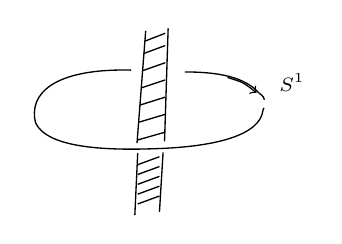
\begin{tikzpicture}[x=.92cm,y=.78cm,line width=.48pt,font=\scriptsize]
\draw (-.17,-1.54)--(-.13,-.53) (-.14,-.37)--(-.02,1.46);
\draw (.17,-1.49)--(.22,-.52) (.24,-.34)--(.29,1.50);
\foreach \y in {-.32,-.03,.25,.53,.81,1.09,1.29} {
  \draw ({-.14+.064*(\y+.37)},\y)--(.25,{\y+.13});
}
\foreach \y in {-1.36,-1.20,-1.04,-.88,-.72} {
  \draw (-.13,\y)--(.17,{\y+.13});
}
\draw (-.22,.82) .. controls (-1.31,.85) and (-1.64,.42) .. (-1.54,-.04)
  .. controls (-1.38,-.44) and (-.61,-.49) .. (.10,-.46)
  .. controls (.95,-.43) and (1.56,-.24) .. (1.60,.17);
\draw (.52,.79) .. controls (1.12,.79) and (1.39,.65) .. (1.55,.44);
\draw[dashed] (1.55,.44) .. controls (1.65,.37) and (1.64,.25) .. (1.60,.17);
\draw[->] (1.11,.70) .. controls (1.33,.62) .. (1.51,.45);
\node at (2.00,.62) {$S^1$};
\end{tikzpicture}}\endgroup}
\end{GelfandAdjacentEvidence}
\begin{GelfandAdjacentEvidence}{GELFAND-P001035}{5}

\SourceFigure{GELFAND-P001035}{circle-map}{%
Получаем отобр. $S^1\to\mathcal R$.\par
$\Rightarrow$ стабильность (?)}
\end{GelfandAdjacentEvidence}
\begin{GelfandAdjacentEvidence}{GELFAND-P001035}{6}


(13) \uwave{При обходе вокруг нити частица может изменить тип (стать другой)}

\dashuline{Пример}: может изменить электрич. заряд.
\SourceFigure{GELFAND-P001035}{parallel-strokes}{$\vert\quad\vert$}
\end{GelfandAdjacentEvidence}
\begin{GelfandAdjacentEvidence}{GELFAND-P001035}{7}


$\forall$ вакуума $\phi\in\mathcal R$ $\exists$ группа ненарушенных симметрий $H_\phi$ (сохр. $\phi$)

\dashuline{Предположение}:
\begin{equation*}
H_\phi=K\times U(1)\subset\widetilde G
\tag{14}
\end{equation*}
(здесь $U(1)$ --- эл.-магн. группа).

Пусть в $\widetilde G$ есть элемент $\alpha\in\widetilde G$, переворачивающий $U(1)$:
\begin{equation*}
\text{\uwave{\(\alpha u\alpha^{-1}=u^{-1}\)}}\qquad \text{при }u\in U(1)
\tag{15}
\end{equation*}

(16) \underline{Утв.} Тогда $\exists$ топ. нетрив. нить (и даже реш.), при обходе к-рой частица меняет заряд.

\begin{center}--- $\cdot$ ---\end{center}

О чётности.
\Unclear{GELFAND-P001035}{mirror-cancel}{Зачёркнутый знак неразборчив.}
\end{GelfandAdjacentEvidence}
\begin{GelfandAdjacentEvidence}{GELFAND-P001035}{8}

Гип.: есть зеркальное вещество.
\SourceFigure{GELFAND-P001035}{mirror-abbreviation}{«О чётности», затем «Гип.».}
\end{GelfandAdjacentEvidence}
\begin{GelfandAdjacentEvidence}{GELFAND-P001035}{9}


Внутри Солнца есть планета из зеркального вещества, к-рая слабо взаимод., но гравит. влияет $\Rightarrow$ объясняет нек-рые эксперименты.

(17) \underline{Утв.} 1) $\exists$ больших объед., включ. зеркальные частицы

2) Неразборчивая зачёркнутая запись после «2)».
\Unclear{GELFAND-P001035}{cancel17}{Неразборчивая зачёркнутая запись после «2)».}
\end{GelfandAdjacentEvidence}
\begin{GelfandAdjacentEvidence}{GELFAND-P001035}{10}

$\exists$ нити, при обходе к-рых частицы превр. в зеркальные.

Взаимод. наших и зерк. частиц \uwave{слабое} (взаимод. через тяжёлые бозоны; если пренебречь --- лагранжиан распадётся).
\SourceFigure{GELFAND-P001035}{overwritten-prefix}{Начало «пренебречь» написано поверх прежних штрихов.}
\end{GelfandAdjacentEvidence}
\begin{GelfandAdjacentEvidence}{GELFAND-P001035}{11}


Это \underline{не} античастицы; есть зеркальные фотоны, зеркальный заряд и т.д.

\uwave{Связь очень слаба}.

\uwave{Нить таких объед}. Эффект.
\SourceFigure{GELFAND-P001035}{thread-heading}{Подчёркнуто «Нить таких объед.».}
\end{GelfandAdjacentEvidence}
\begin{GelfandAdjacentEvidence}{GELFAND-P001035}{12}


\SourceFigure{GELFAND-P001035}{star-thread-observer}{%
\begingroup\color{black}\GelfandFitDiagram{\begin{tikzpicture}[x=.83cm,y=.79cm,line width=.52pt,font=\scriptsize]
\draw (-.14,1.67)--(.14,1.67)
      (-.09,1.52)--(.09,1.81) (-.09,1.81)--(.09,1.52);
\node[anchor=west] at (.19,1.69) {звезда};
\draw (-1.0,-.06)--(2.92,1.27);
\node[anchor=west] at (2.97,1.30) {Нить};
\fill (1.71,-.39) circle (.032);
\node[anchor=west] at (1.79,-.32) {мы};
\end{tikzpicture}}\endgroup}
\end{GelfandAdjacentEvidence}
\begin{GelfandAdjacentEvidence}{GELFAND-P001035}{13}

Перестаём видеть звезду, т.к. её фотоны
\Unclear{GELFAND-P001035}{cancel-bottom}{Неразборчивая зачёркнутая запись перед «стан.».}
\end{GelfandAdjacentEvidence}
\begin{GelfandAdjacentEvidence}{GELFAND-P001035}{14}

стан. зеркальными.

Динамика квазиклассическая, к-рая применима, т.к. мы далеко от нити.

Считается, что нити должны были сохраниться с ранней Вселенной.
\SourceFigure{GELFAND-P001035}{last-verb}{Последняя фраза начинается «Считается».}
\end{GelfandAdjacentEvidence}



\Needspace{7\baselineskip}
\begin{GelfandAdjacentEvidence}{GELFAND-P001036}{1}
\SourcePage{GELFAND-P001036}{8}
Неясно, сущ. ли \underline{квантово} стабильные нити (классически они стабильны).

При движении нити звёзды должны заменяться (на зеркальные).
\SourceFigure{GELFAND-P001036}{line-02-verb}{Глагол «заменяться».}
\end{GelfandAdjacentEvidence}
\begin{GelfandAdjacentEvidence}{GELFAND-P001036}{2}

\SourceFigure{GELFAND-P001036}{line-02-parenthesis}{В скобках: «на зеркальные».}
\end{GelfandAdjacentEvidence}
\begin{GelfandAdjacentEvidence}{GELFAND-P001036}{3}


\uwave{Хлопов}: метагалактики пополам [чтение вероятно]\textsuperscript{?}
\Unclear{GELFAND-P001036}{line-03-phrase}{метагалактики пополам [чтение вероятно]}
\end{GelfandAdjacentEvidence}
\begin{GelfandAdjacentEvidence}{GELFAND-P001036}{4}

и ничего не изменится;
ед. шанс --- квазары; они
специальные [чтение вероятно]\textsuperscript{?},
\Unclear{GELFAND-P001036}{line-04-adjective}{специальные [чтение вероятно]}
\end{GelfandAdjacentEvidence}
\begin{GelfandAdjacentEvidence}{GELFAND-P001036}{5}

но у них есть характерный ритм изменения.

Есть \underline{препринт}: 1 квазар за 100 лет
\uwave{резко изменил свою светимость}.
\SourceFigure{GELFAND-P001036}{preprint-or-precedent}{Подчёркнуто «препринт».}
\end{GelfandAdjacentEvidence}


\dashuline{Замеч. Хлопова}: объя\underline{сняется}, \underline{если} нить прошла.


\Needspace{7\baselineskip}
\begin{GelfandAdjacentEvidence}{GELFAND-P001037}{1}
\SourcePage{GELFAND-P001037}{unlabelled}
\underline{20/$\overline{\underline{\mathrm{IX}}}$-82.}\qquad \uuline{Сем. Гельфанда.}

\uuline{Синай.}

\underline{Темы} (по физике)

1. Ренорм группа.

2. Дебаевское экранирование как основной механизм фазовых переходов систем с непрерывной симметрией.

3. Калибровочные модели.

4. Гравитация, суперсимметрия, супергравитация.

\uuline{А. А. Мигдал.}

5. Решётчатые модели.
\Unclear{GELFAND-P001037}{topic-five-cancellation}{Неразборчивое зачёркнутое выражение в скобках.}
\end{GelfandAdjacentEvidence}
\begin{GelfandAdjacentEvidence}{GELFAND-P001037}{2}


6. Струны.

7. Большие $N$ ($N$ --- ранг калибровочной группы):
\[
u(\infty)=\mathrm{sp}(\infty)=O(\infty)
\]
\SourceFigure{GELFAND-P001037}{large-n-symbols}{Обозначения в рукописи: \(u(\infty),\mathrm{sp}(\infty),O(\infty)\).}
\end{GelfandAdjacentEvidence}
\begin{GelfandAdjacentEvidence}{GELFAND-P001037}{3}


8. Кварки и лептоны. \dashuline{Единые} теории.

9. Локализация Андерсона.

10. Универсальность Фейгенбаума.
\SourceFigure{GELFAND-P001037}{feigenbaum-overwrite}{В фамилии «Фейгенбаума» буква «н» написана поверх прежних штрихов.}
\end{GelfandAdjacentEvidence}


\uuline{Синай} \underline{о п. 10.}

\uwave{В 1-мерном случае}: Пусть
\[
\begin{aligned}
[-1,1]&\longrightarrow[-1,1]\\
x&\longmapsto f(x;\mu)
\end{aligned}
\]
\[
\begin{aligned}
\text{а)}\quad &f(-x;\mu)=f(x;\mu)\\
\text{б)}\quad &f(0;\mu)=1.
\end{aligned}
\]
[Справа:] \underline{Пример}: $f(x,\mu)=1-\mu x^2$, $1<\mu<2$.


\Needspace{7\baselineskip}
\begin{GelfandAdjacentEvidence}{GELFAND-P001038}{1}
\SourcePage{GELFAND-P001038}{9}
\Unclear{GELFAND-P001038}{top-cancellation}{Зачёркнутое слово, возможно, «Рассм.».}
\end{GelfandAdjacentEvidence}
\begin{GelfandAdjacentEvidence}{GELFAND-P001038}{2}

[вставлено над строкой] Сущ. послед. знач. $\mu_n$:
\begin{equation*}
\forall\mu:\quad \mu_n<\mu<\mu_{n+1}\quad\Rightarrow\quad
\exists\ \text{устойч. траект. периода }2^n.
\tag{1}
\end{equation*}
Рассм.
\begin{equation*}
\frac{\mu_n-\mu_{n+1}}{\mu_{n-1}-\mu_n}
\underset{n\to\infty}{\longrightarrow}\delta^{-1},\qquad
\delta\approx4{,}6992
\tag{2}
\end{equation*}
\SourceFigure{GELFAND-P001038}{feigenbaum-constant}{В рукописи: \(\delta\approx4{,}6992\).}
\end{GelfandAdjacentEvidence}
\begin{GelfandAdjacentEvidence}{GELFAND-P001038}{3}


Мн-во [вставлено над строкой] сем-в отобр., для к-рых $\exists$ послед. $\mu_n$ ---
\underline{открытое мн-во} в пр-ве отобр.
\SourceFigure{GELFAND-P001038}{family-insertion}{«сем-в» со знаком внесения.}
\end{GelfandAdjacentEvidence}
\begin{GelfandAdjacentEvidence}{GELFAND-P001038}{4}


\uwave{Есть обобщ. для дифф. ур-й}.

\begin{equation*}
\frac{dx_i}{dt}=f(x_1,\ldots,x_r,\mu),\qquad1\le i\le r
\tag{3}
\end{equation*}
\Unclear{GELFAND-P001038}{sinai-eq3-indices}{В последнем аргументе \(x_r\) индекс похож на \(r\) в правой границе, но штрихи мелкие.}
\end{GelfandAdjacentEvidence}
\begin{GelfandAdjacentEvidence}{GELFAND-P001038}{5}


(4) $\mu_n$, $\mu_n<\mu<\mu_{n+1}$ $\Rightarrow$ есть периодич. траект., к к-рой всё притяг.,
кроме конечного числа замкнутых траекторий.

\SourceFigure{GELFAND-P001038}{orbit-progression}{%
\begingroup\color{black}\GelfandFitDiagram{\begin{tikzpicture}[x=.75cm,y=.72cm,font=\scriptsize,line width=.45pt]
\draw[rotate around={38:(-3.41,0)}] (-3.41,0) ellipse [x radius=.46,y radius=.26];
\draw[->] (-2.90,-.06)--(-2.46,-.06);
\begin{scope}[shift={(-1.97,-.02)},rotate=43]
\draw (0,0) ellipse [x radius=.50,y radius=.28];
\draw (.01,.09) ellipse [x radius=.40,y radius=.20];
\draw (-.39,.12)--(-.22,.25);
\end{scope}
\draw[->] (-1.39,-.05)--(-.87,-.05);
\begin{scope}[shift={(-.32,-.02)},rotate=37]
\draw (0,0) ellipse [x radius=.50,y radius=.35];
\draw (-.09,.06) ellipse [x radius=.39,y radius=.23];
\draw (.10,.01) ellipse [x radius=.38,y radius=.19];
\end{scope}
\draw[->] (.24,.01)--(.98,.04);
\node at (1.56,-.02) {$\cdots$};
\draw[->] (2.00,-.03)--(2.60,-.03);
\node[anchor=west] at (2.75,-.02) {\uwave{тор}.};
\end{tikzpicture}}\endgroup\par
Точный ход линий в двух средних контурах неясен.}
\end{GelfandAdjacentEvidence}
\begin{GelfandAdjacentEvidence}{GELFAND-P001038}{6}


\begin{equation*}
\mu_n-\mu_\infty\sim C(f)\delta^{-n},
\tag{5}
\end{equation*}
где $\delta$ --- та же, что и выше,
и мн-во таких систем \uwave{открыто}.

\uwave{Больше пар.}

(6) $\mu_1,\mu_2$ $\Rightarrow$ \uwave{бывает утроение периодов}
(и тоже найдена $\mathrm{const}$).

\begin{center}--- $\cdot$ ---\end{center}

Для ф-и $f$ бывает сложное функц. ур-е:
\begin{equation*}
-\frac1\alpha f(f(\alpha x))=f(x)
\tag{7}
\end{equation*}
\uwave{Решается}: многочлен (10-й степ.) и численно на машине.

Ренормгруппа возникает из линеаризации этого ур-я.

(8) \underline{Вопрос}: что будет при $\mu>\mu_\infty$ с вект. полем?

Для отображений известно: возникает отобр. с эргодич. инвар. мерой
(перемешивание и пр. $\Rightarrow$ начало стохастичности).

\uuline{А. А. Мигдал.}

Дано поле $\varphi(x)$ со знач. в алгебре $u(N)$, т. е. $(\varphi_{ij})$ ---
антиэрмитова матрица,
\begin{equation*}
\varphi_{ij}(x)=-\varphi_{ji}^{*}(x)\qquad\text{или}\qquad
\varphi(x)=-\varphi^{+}(x),\qquad\text{(для определённости)}
\tag{1}
\end{equation*}

При $N\to\infty$ есть [вставлено над строкой] универс. предел
(но не гауссов!) и для предела есть нек-рые ур-я и
\Unclear{GELFAND-P001038}{migdal-prose-cancellation}{Неразборчивая зачёркнутая запись перед «наблюдения».}
\end{GelfandAdjacentEvidence}
\begin{GelfandAdjacentEvidence}{GELFAND-P001038}{7}

наблюдения.
\SourceFigure{GELFAND-P001038}{universal-insertion}{«универс.» вписано над строкой.}
\end{GelfandAdjacentEvidence}


\begin{equation*}
L=\operatorname{tr}\left[\frac12(\partial_\mu\varphi)^2+U(\varphi)\right]N/\lambda,
\tag{2}
\end{equation*}
$U(\varphi)$ --- полином 4-й степени --- например, $\varphi^4$.

(3) $\bullet$ Классич. ур-е $\dfrac{\delta S}{\delta\varphi}=0$, где
\begin{equation*}
S=\int L\,d^4x
\tag{4}
\end{equation*}
(пр-во евклидово)


\Needspace{7\baselineskip}
\begin{GelfandAdjacentEvidence}{GELFAND-P001039}{1}
\SourcePage{GELFAND-P001039}{unlabelled}
Рассм. ур-е
\begin{equation*}
\frac{\partial\varphi}{\partial\tau}+\frac{\delta S}{\delta\varphi}=J(x,\tau),
\tag{5}
\end{equation*}
\SourceFigure{GELFAND-P001039}{noise-under-j}{%
$\underset{\text{случайный ток }=\text{ гауссов случайный шум}}{\uparrow}$}
\end{GelfandAdjacentEvidence}
\begin{GelfandAdjacentEvidence}{GELFAND-P001039}{2}


причём
\begin{equation*}
\langle J^{ik}(x,\tau)J^{i'k'}(x',\tau')\rangle
=\delta^{ii'}\delta^{kk'}\delta(x-x')\delta(\tau-\tau')
\tag{6}
\end{equation*}
(это их полностью опис., т. к. они гауссовы)

(7) \underline{Утв.} Пусть $\varphi|_{\tau=0}=0$.
Тогда решение $\varphi(x,\tau)$ облад. тем св-вом, что если
\[
\overline Q=\frac1T\int_0^T Q(\varphi(x,\tau))\,d\tau
\]
[Справа:] ($Q$ --- ф-л; напр. $Q=\operatorname{tr}(\varphi^2)$).
инвар. отн. группы при действии --- присоед.
\[
\varphi\longmapsto S^{+}\varphi S
\]
то $\overline Q$ даётся ф-лой
\begin{equation*}
\overline Q=\int D\varphi\,\exp(-S)\,Q(\varphi(x))\Big/\int D\varphi\,e^{-S}
\tag{8}
\end{equation*}

Вместо (8) рассматриваем (5).

\textcircled{1}\quad \uwave{Самоусреднение}. Рассм.
\begin{equation*}
G(1,\ldots,n)=\frac{\operatorname{tr}}N(\varphi(1)\ldots\varphi(n))
\tag{9}
\end{equation*}
Здесь $(T,x_1)\mapsto1$, $\ldots$ (для краткости);
\underline{$T$ фиксировано}.
\Unclear{GELFAND-P001039}{short-time-correction}{Первый знак в паре переписан, наиболее вероятно \(T\).}
\end{GelfandAdjacentEvidence}
\begin{GelfandAdjacentEvidence}{GELFAND-P001039}{3}


Тогда
\begin{equation*}
\lim_{T\to\infty}G_T(1,\ldots,n,T)=\overline G+O(1/N),
\qquad\text{(при }N\to\infty\text{)}
\tag{10}
\end{equation*}
\Unclear{GELFAND-P001039}{eq10-raised-sign}{У \(G\) видна нижняя помета, похожая на \(T\). После \(n\) видны косой штрих и приподнятый знак, похожий на \(T\).}
\end{GelfandAdjacentEvidence}
\begin{GelfandAdjacentEvidence}{GELFAND-P001039}{4}


[Справа:] здесь $\overline G(1,\ldots,n)$ --- ф-я точек, не завис. от $T$ и $N$.

(убывание флуктуаций).

\uwave{Точки совп.}:
$\dfrac1N\operatorname{tr}\varphi^n=\dfrac1N\sum_\lambda\lambda^n$ и дисперсия уменьшается.

В общ. случае возник. $\sum$ членов с одинак. распр. вероятностей.

Итак: следы \uwave{не флуктуируют}.

\textcircled{2}\quad При $N=\infty$ можно сделать редукцию:
\begin{equation*}
\varphi(x)\longmapsto e^{ipx}\varphi(0)e^{-ipx},\qquad
p=i\,\partial/\partial x
\tag{11}
\end{equation*}
$p$ Неразборчивый знак после \(p\) зачёркнут.
\Unclear{GELFAND-P001039}{after-p-cancellation}{Неразборчивый знак после \(p\) зачёркнут.}
\end{GelfandAdjacentEvidence}
\begin{GelfandAdjacentEvidence}{GELFAND-P001039}{5}

можно заменить на матрицу из картан. алгебры (диаг.)

\begin{equation*}
\widetilde J(x,t)=e^{ip_\mu x^\mu}j(t)e^{-ip_\mu x^\mu},
\tag{12}
\end{equation*}
\Unclear{GELFAND-P001039}{eq12-x-corrections}{В обоих показателях нижние индексы у \(x\) зачёркнуты и сверху вписано \(\mu\). Зачёркнутые индексы неразборчивы.}
\end{GelfandAdjacentEvidence}
\begin{GelfandAdjacentEvidence}{GELFAND-P001039}{6}


[Справа:] $p_\mu$ --- диаг. матрица,
$p=\operatorname{diag}(p_\mu^1,\ldots,p_\mu^N)$

$j(t)$ --- гаусс. шум

\SourceFigure{GELFAND-P001039}{repeated-noise-arrow}{%
$j(t)$ --- гауссов шум; \quad $\swarrow$ к (13)}
\end{GelfandAdjacentEvidence}
\begin{GelfandAdjacentEvidence}{GELFAND-P001039}{7}


\Unclear{GELFAND-P001039}{random-p-cancellation}{Справа зачёркнута запись, начинающаяся с \(p\).}
\end{GelfandAdjacentEvidence}
\begin{GelfandAdjacentEvidence}{GELFAND-P001039}{8}

$p^\mu$ --- случ. велич., (не зав. ни от $t$, ни от $x$)
\Unclear{GELFAND-P001039}{random-p-indices}{Надстрочный знак похож на \(\mu\). Нижний штрих мог быть зачёркнутым индексом.}
\end{GelfandAdjacentEvidence}


\begin{equation*}
\langle j^{ik}(t),j^{i'k'}(t')\rangle=\delta(t-t')\delta^{ii'}\delta^{kk'}
\tag{13}
\end{equation*}


\Needspace{7\baselineskip}
\begin{GelfandAdjacentEvidence}{GELFAND-P001040}{1}
\SourcePage{GELFAND-P001040}{10}
$p^j$ --- случ. величины, распред. [вписано сверху] (по Гауссу)
с плотн. $\exp(-p^2/\Lambda^2)$ (с дисп. $1/\Lambda^2$)
\Unclear{GELFAND-P001040}{top-p-index}{Верхний индекс похож на \(j\); возможно \(i\).}
\end{GelfandAdjacentEvidence}
\begin{GelfandAdjacentEvidence}{GELFAND-P001040}{2}

\SourceFigure{GELFAND-P001040}{top-density-variance}{В рукописи \(\exp(-p^2/\Lambda^2)\) и «с дисп. \(1/\Lambda^2\)».}
\end{GelfandAdjacentEvidence}
\begin{GelfandAdjacentEvidence}{GELFAND-P001040}{3}


где $\underset{\substack{\vert\\\text{\uwave{радиус обрезания}}}}{\Lambda}\to\infty$
(после того, как $N\to\infty$).

В пределе при
\[
\begin{gathered}
N\to\infty\\
\Lambda\to\infty
\end{gathered}
\]
получится тот же белый шум $J(x,t)$ (см. выше).

Сведётся к обыкн. ур-ю (случ. матрице).

\SourceFigure{GELFAND-P001040}{equivalence-cancellation}{\sout{Эквивалентность}}
\end{GelfandAdjacentEvidence}
\begin{GelfandAdjacentEvidence}{GELFAND-P001040}{4}


\underline{Утверждение}.
\[
\underset{\substack{\vert\\\text{по }J}}{G}
-\underset{\substack{\vert\\\text{по }\widetilde J}}{\widetilde G}
\to0
\]
\begin{equation*}
\frac{\partial\widetilde\varphi}{\partial\tau}
+\frac{\delta S}{\delta\widetilde\varphi}=\widetilde J(x,\tau)
\tag{14}
\end{equation*}

Решается:
\begin{equation*}
\varphi(x,\tau)=e^{ipx}\bar\varphi(t)e^{-ipx},\qquad\text{где}
\tag{15}
\end{equation*}
\SourceFigure{GELFAND-P001040}{eq15-time}{Слева \(\tau\), у \(\bar\varphi\) аргумент \(t\).}
\end{GelfandAdjacentEvidence}
\begin{GelfandAdjacentEvidence}{GELFAND-P001040}{5}


\begin{equation*}
\frac{\partial\bar\varphi}{\partial\tau}
+[p[p\bar\varphi]]+U(\bar\varphi)=\widetilde j
\tag{16}
\end{equation*}
\SourceFigure{GELFAND-P001040}{eq16-notation}{В скобках запятых не видно, у \(U\) не виден штрих.}
\end{GelfandAdjacentEvidence}
\begin{GelfandAdjacentEvidence}{GELFAND-P001040}{6}


\[
p=\operatorname{diag}(p_1,\ldots,p_N)
\]
Итак, завис. от координат устранена.

Интегралы перех. в интеграл:
\begin{equation*}
\bar Q=\int dp\int d\varphi\,\exp\bigl(\operatorname{tr}\bigl(([p,\varphi]^2+U_\Lambda(\varphi)\bigr)\bigr)Q(\varphi)
\tag{17}
\end{equation*}
\SourceFigure{GELFAND-P001040}{eq17-parentheses}{Одна открывающая скобка после \(\exp\), две после \(\operatorname{tr}\), три закрывающие после \(\varphi\) в \(U_\Lambda(\varphi)\).}
\end{GelfandAdjacentEvidence}
\begin{GelfandAdjacentEvidence}{GELFAND-P001040}{7}


Точнее,

\Unclear{GELFAND-P001040}{crossed-before-eq18}{Зачёркнутая строка, возможно, начиналась с \((18)\) и \(\bar Q\).}
\end{GelfandAdjacentEvidence}
\begin{GelfandAdjacentEvidence}{GELFAND-P001040}{8}

\begin{equation*}
\begin{aligned}
\underset{\substack{\uparrow\\\text{по траекториям (см. выше)}}}{\bar Q}
&=\lim_{\Lambda\to\infty}\lim_{N\to\infty}M_p\\
&\quad\Bigl\{\int_{U(N)}d\varphi\,\exp\bigl(\operatorname{tr}\bigl(([p,\varphi]^2+U(\varphi)\bigr)\bigr)Q(\varphi)\Bigr\}
\end{aligned}
\tag{18}
\end{equation*}
\SourceFigure{GELFAND-P001040}{eq18-parentheses}{Последовательность скобок совпадает с (17).}
\end{GelfandAdjacentEvidence}
\begin{GelfandAdjacentEvidence}{GELFAND-P001040}{9}


\underline{Надо вычислить}:
\begin{equation*}
\lim_{N\to\infty}\frac{1}{N^2}\ln
\int_{U(N)}\prod_{\mu=1}^{4}dU_\mu\,
\exp\bigl(-\beta N\sum_{\mu,\nu}\operatorname{tr}(U_\mu U_\nu U_\mu^+U_\nu^+)\bigr)=F(\beta)
\tag{19}
\end{equation*}
\SourceFigure{GELFAND-P001040}{log-insertion}{Перед интегралом вписано \(\tfrac{1}{N^2}\ln\).}
\end{GelfandAdjacentEvidence}
\begin{GelfandAdjacentEvidence}{GELFAND-P001040}{10}

(своб. энергия)

$dU_\mu$ --- мера Хаара

(Статсумма решёт. теории [вписано сверху] (поля) при $N\to\infty$ в 4-мерном пр-ве)

Это $\sim$ теория поля

\underline{Вычислена}:
\begin{equation*}
\int dU\,\exp\bigl(\beta N\operatorname{tr}(Uh+h^+U^+)
\tag{20}
\end{equation*}
для произв. матрицы $h$
\SourceFigure{GELFAND-P001040}{eq20-parentheses}{В конце формулы видна только одна закрывающая скобка.}
\end{GelfandAdjacentEvidence}
\begin{GelfandAdjacentEvidence}{GELFAND-P001040}{11}


(сложное выражение)

Впервые. \uwave{Пиризен}, \uwave{Гросс}; затем \uwave{Фатеев}.
\Unclear{GELFAND-P001040}{bottom-surname}{Первая фамилия похожа на «Пиризен»; первая гласная не вполне ясна.}
\end{GelfandAdjacentEvidence}



\Needspace{7\baselineskip}
\begin{GelfandAdjacentEvidence}{GELFAND-P001041}{1}
\SourcePage{GELFAND-P001041}{unlabelled}
\underline{27/$\overline{\underline{\mathrm{IX}}}$-82 г.}\qquad
\uuline{Сем. Гельфанда.}

\uuline{Фукс.}

\uwave{Представл. группы диффеом. окружности}.

(1) Рассм. алгебру $\{e_i,\ i\in\mathbb Z\}$
\[
\relax[e_i,e_j]=(j-i)e_{i+j}.
\]
(векторных полей на окружности)
\SourceFigure{GELFAND-P001041}{cancelled-algebra-name}{%
[Справа:] \sout{(алг. Вирасоро)}}
\end{GelfandAdjacentEvidence}
\begin{GelfandAdjacentEvidence}{GELFAND-P001041}{2}


Есть единств. центр. расширение (Гельф.-Фукс):
\begin{equation*}
\{e_i,z\},\quad
\left.
\begin{gathered}
\relax[e_i,e_j]=\begin{cases}
(j-i)e_{i+j},&i+j\ne0,\\
\text{---''---}+\frac{1}{12}(j^3-j)z,&i+j=0,
\end{cases}\\
[e_i,z]=0,\quad\forall i
\end{gathered}
\right]\quad\begin{gathered}\text{алгебра}\\\text{Вирасоро}\end{gathered}
\tag{2}
\end{equation*}

\dashuline{Представления алг. Вирасоро}.

(3) \uwave{Модули Верма},
\SourceFigure{GELFAND-P001041}{verma-grading}{%
\begingroup\color{black}\GelfandFitDiagram{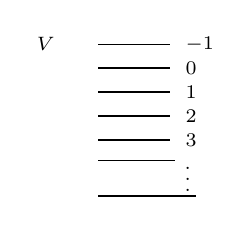
\begin{tikzpicture}[x=.85cm,y=.82cm,font=\scriptsize,line width=.50pt]
\node at (-.78,.01) {$V$};
\foreach \y/\weight in {0/-1,-.37/0,-.74/1,-1.11/2,-1.48/3} {
  \draw (0,\y)--(1.08,\y);
  \node[anchor=west] at (1.16,\y) {$\weight$};
}
\draw (0,-1.80)--(1.15,-1.80);
\node at (1.34,-1.97) {$\vdots$};
\draw (0,-2.35)--(1.46,-2.35);
\end{tikzpicture}}\endgroup}
\end{GelfandAdjacentEvidence}
\begin{GelfandAdjacentEvidence}{GELFAND-P001041}{3}

град. Зачёркнутый знак неразборчив.
\Unclear{GELFAND-P001041}{verma-overwritten-mark}{Зачёркнутый знак неразборчив.}
\end{GelfandAdjacentEvidence}
\begin{GelfandAdjacentEvidence}{GELFAND-P001041}{4}

модули, огранич. снизу

(градуир. полуограниченные)

(4) Подалгебра $\{e_i,\ i>0\}$;

\underline{Модуль Верма}: если есть [вписано сверху] такой вект. $v$, что
\SourceFigure{GELFAND-P001041}{basis-insertion}{\sout{базис}}
\end{GelfandAdjacentEvidence}
\begin{GelfandAdjacentEvidence}{GELFAND-P001041}{5}

\[
\{v,\ e_1v,\ e_1^2v,\ e_2v,\ e_1^3v,\ e_2e_1v,\ e_3v,\ \ldots\}\quad\text{---}
\]

(5) --- базис, и $e_{-j}v=0$ при $j>0$.
(достат. $e_{-1}v=e_{-2}v=0$)

Фиксируем компл. числа $h$ и $c$.
\begin{equation*}
\underline{e_0v=hv,\quad zv=cv}
\tag{6}
\end{equation*}
(доп. условие). ---

По $h,c$ однозн. восстанавливается. Обозначение $V_{h,c}$.

\uwave{Постр. модуль} $\{f_j\mid j\in\mathbb Z\}$
\Unclear{GELFAND-P001041}{module-horizontal-marks}{Две черты над записью: одна правее \(f_j\), другая над \(\mathbb Z\). Их связь с записью неясна.}
\end{GelfandAdjacentEvidence}
\begin{GelfandAdjacentEvidence}{GELFAND-P001041}{6}

(вспомогательный) по ф-лам:
\begin{equation*}
e_if_j=[j+\mu-(i+1)\lambda]f_{i+j}
\tag{7}
\end{equation*}

(\uwave{Можно предст. себе}:
\begin{equation*}
e_i=z^{i+1}\frac{d}{dz},\quad f_j=z^{j+\mu}dz^{-\lambda})
\tag{8}
\end{equation*}
Обозн. его $\overline W_{\lambda,\mu}$
\SourceFigure{GELFAND-P001041}{module-symbol}{Видна черта над \(W\).}
\end{GelfandAdjacentEvidence}
\begin{GelfandAdjacentEvidence}{GELFAND-P001041}{7}


Рассмотрим последовательности.
\begin{equation*}
\begin{gathered}
\cdots\wedge f_{j_3}\wedge f_{j_2}\wedge f_{j_1}\\
\cdots<j_3<j_2<j_1
\end{gathered}
\tag{9}
\end{equation*}
\[
\cdots\wedge f_{-4}\wedge\underset{-3}{f_2}\wedge\underset{-2}{f_5}\wedge\underset{-1}{f_9}
\]
\SourceFigure{GELFAND-P001041}{wedge-last-index}{Последний множитель \(f_9\), под ним \(-1\).}
\end{GelfandAdjacentEvidence}
\begin{GelfandAdjacentEvidence}{GELFAND-P001041}{8}


(до нек-рого места номера идут подряд; если след. заменить на

идущие подряд то Короткая зачёркнутая запись неразборчива.
\Unclear{GELFAND-P001041}{bottom-cancelled-mark}{Короткая зачёркнутая запись неразборчива.}
\end{GelfandAdjacentEvidence}

кончится на $-1$

$e_i$ прим. по очереди справа; получ. сумму беск. числа слагаемых.

Если возникающее $f_{i+j}$ уже есть, то произв. равно $0$.


\Needspace{7\baselineskip}
\begin{GelfandAdjacentEvidence}{GELFAND-P001042}{1}
\SourcePage{GELFAND-P001042}{11}

Реально получ. конечная сумма.

Так опред. $e_i$ при $i\ne0$, а $e_0$ нельзя.

\[
e_0=[e_{-1},e_1]\quad\text{— по этой ф-ле опр. }e_0.
\]
\[
e_0=[e_{-2},e_2]\quad\text{— другой коэфф. получается! — противоречие.}
\]
\SourceFigure{GELFAND-P001042}{overwritten-e0}{Начальный знак второго равенства переписан; читается как \(e_0\).}
\end{GelfandAdjacentEvidence}
\begin{GelfandAdjacentEvidence}{GELFAND-P001042}{2}


Но: одновр. $e_0$ и $z$ можно опред. (и однозначно!).

$z$ — умножение на число.

(см. раб. Фейгин, Фукс; ФА, 1982, $N=2$)

$e_0$ — умн. на $h+n$,\quad
$h=\tfrac12\mu(\mu-2\lambda+1)$.\quad (?)
\SourceFigure{GELFAND-P001042}{highest-weight-formula}{В рукописи \(+1\) и справа «(?)».}
\end{GelfandAdjacentEvidence}
\begin{GelfandAdjacentEvidence}{GELFAND-P001042}{3}


(10) \uwave{Старший вектор}:
\[
\underset{\text{(все подряд)}}{\cdots f_{-3}\wedge f_{-2}\wedge f_{-1}}
\]
Если неприводим, то явл. модулем Верма́.

\underline{Кац.}\quad (Lect. Notes Phys., 1979):

Какие модули Верма $\overline V_{h,c}$ неприводимы?
\SourceFigure{GELFAND-P001042}{verma-symbol}{В вопросе над \(V\) стоит черта.}
\end{GelfandAdjacentEvidence}
\begin{GelfandAdjacentEvidence}{GELFAND-P001042}{4}


\begin{equation*}
\begin{aligned}
\overline\Phi_{k_1,k_2}(h,c)
={}&\Bigl(h-\frac{k_1^2-1}{24}(c-13)+\frac{k_1k_2-1}{2}\Bigr)
    \Bigl(h-\frac{k_2^2-1}{24}(c-13)+\frac{k_1k_2-1}{2}\Bigr)+\\
&+\frac{(k_1^2-k_2^2)^2}{16}
\end{aligned}
\tag{11}
\end{equation*}
\SourceFigure{GELFAND-P001042}{kac-polynomial-sign}{Черта над \(\Phi\); перед первой дробью минус.}
\end{GelfandAdjacentEvidence}
\begin{GelfandAdjacentEvidence}{GELFAND-P001042}{5}

\SourceFigure{GELFAND-P001042}{kac-second-factor}{Знак перед последней единицей пересекает вертикальную линию сетки; читается как минус.}
\end{GelfandAdjacentEvidence}
\begin{GelfandAdjacentEvidence}{GELFAND-P001042}{6}


(12) \underline{Теор.} $V_{h,c}$ приводим
$(\Leftrightarrow)\ \exists$ целые $k_1,k_2>0$,
$\underline{\overline\Phi}_{k_1,k_2}(h,c)=0$.
\Unclear{GELFAND-P001042}{kac-theorem-symbol}{Под \(\Phi\) видна черта. Короткий верхний штрих может быть частью написания буквы.}
\end{GelfandAdjacentEvidence}
\begin{GelfandAdjacentEvidence}{GELFAND-P001042}{7}


\begin{center}— . —\end{center}
\[
c=0\quad\Rightarrow\quad h=\frac{m^2-1}{24}
\]
\begin{center}— . —\end{center}

\underline{2-я конструкция}.

(13) Рассм. многочлены от переменных
\[
\begin{array}{ccccc}
&x_1,&x_2,&x_3,&\ldots\\
\text{весов}&1,&2,&3,&\ldots
\end{array}
\]
Есть 2 преобр.: умн. на $x_i$ и $\partial/\partial x_i$.

Положим
\begin{equation*}
F_k=\sum_i x_i\frac{\partial}{\partial x_{i+k}}.
\tag{14}
\end{equation*}

Тогда
\begin{equation*}
e_i=\alpha F_i+
\sum_{\substack{p,q\\p\ne0,\ q\ne0\\p+q=i\\p>q}}F_pF_q
\underset{\text{(если \(i\) чётно)}}{\bigl(+\tfrac12 F_{i/2}^{2}\bigr)},
\quad\alpha\text{ — параметр.}
\tag{15}
\end{equation*}
\Unclear{GELFAND-P001042}{eq15-cancelled-coefficient}{Между знаком \(+\) и \(1/2\) есть зачёркнутый или переписанный знак; возможно, \(2\).}
\end{GelfandAdjacentEvidence}


Здесь
\begin{equation*}
\alpha=\mu-i(\lambda+\tfrac12)
\tag{16}
\end{equation*}


\Needspace{7\baselineskip}
\begin{GelfandAdjacentEvidence}{GELFAND-P001043}{1}
\SourcePage{GELFAND-P001043}{unlabelled}
\underline{Замолодчиков.} \underline{(Саша)}.

(1) Пусть есть поверхность $\vec{x}(\xi^1,\xi^2)$, $\xi^j$ — параметры.

Хотим изучать суммы по пов. разных форм.

Метрика:
\begin{equation*}
G_{ab}=\partial_a\vec{x}\cdot\partial_b\vec{x},\qquad a,b=1,2.
\tag{2}
\end{equation*}
Площадь пов. имеет вид
\begin{equation*}
A=\int\sqrt{\det G_{ab}}\,d\xi
\tag{3}
\end{equation*}
Выраж. \(A\) калибр. инвариантно отн. $\xi^a\to f^a(\xi)$.

Можно добиться выбором калибровки:
\begin{equation*}
G_{ab}=\rho\delta_{ab}
\tag{4}
\end{equation*}
Ур-е движ. с лагранжианом $A$:
\begin{equation*}
\partial_a\partial^a\vec{x}=0,\qquad\text{(ур-е Лапласа)}
\tag{5}
\end{equation*}
\begin{equation*}
\begin{cases}
\partial_1\vec{x}\cdot\partial_2\vec{x}=0,\\
(\partial_1\vec{x})^2=(\partial_2\vec{x})^2
\end{cases}
\tag{6}
\end{equation*}
(из (4)).

Достаточно удовл. (6) на границе $\Rightarrow$ решение даёт миним. поверхность.
\Unclear{GELFAND-P001043}{boundary-abbreviation}{Конец сокращения «удовл.» переписан; первоначальные штрихи неразборчивы.}
\end{GelfandAdjacentEvidence}


Хотим в нек-ром смысле вычислить сумму
\begin{equation*}
\sum_{\text{поверхн.}}e^{-\mu_0^2 A(\text{поверхности})}
\tag{7}
\end{equation*}
Мера — ?

Рассм. сначала
\begin{equation*}
\sum_{\text{путям}}e^{-mL_{\text{пути}}}
\tag{8}
\end{equation*}
$L_{\text{пути}}$ — длина пути ( в обычном смысле; в $d$-мерном евкл. пр-ве)

Для аналогии введём параметрич. задание $\vec{x}(t)$, $t\in(1,2)$. Тогда
\begin{equation*}
L=\int_1^2\sqrt{(\dot{\vec{x}})^2}\,dt,\qquad
\dot{\vec{x}}=\frac{d\vec{x}}{dt}
\tag{9}
\end{equation*}
Минимизируя (9), получим прямые:
\begin{equation*}
\ddot{\vec{x}}=0\qquad\text{(10) — аналог (5)}
\tag{10}
\end{equation*}
Произвол (калибровочный) при заменах $t\mapsto f(t)$
\begin{equation*}
\begin{cases}
\dot{\vec{x}}=\vec{v}\\
\vec{v}^{\,2}=1
\end{cases}
\qquad\text{(11) — аналог (6)}
\tag{11}
\end{equation*}


\Needspace{7\baselineskip}
\begin{GelfandAdjacentEvidence}{GELFAND-P001044}{1}
\SourcePage{GELFAND-P001044}{12}
Есть несколько способов опр. интеграла; все они в итоге оказ. эквив.
\Unclear{GELFAND-P001044}{top-equivalence-verb}{Сокращение в конце строки читается как «оказ.»; возможно «окаж.».}
\end{GelfandAdjacentEvidence}
\begin{GelfandAdjacentEvidence}{GELFAND-P001044}{2}


(12) \shortstack[l]{\uwave{Один:}\\\uwave{способ}}
\quad\uwave{заменяем \(R^d\) решёткой}.
\[
x^\mu=0,\pm1,\pm2,\ldots
\]
Длина \(=\) число шагов.

Сумма сходится и элем. вычисляется (явно!)

(13) \shortstack[l]{\uwave{Другой}\\\uwave{способ}}
\quad Заменим кривую ломаной из $N$ звеньев длины $\Delta$.

Пусть $\Delta$ фиксировано. Получится конечномерный интеграл.

(система шарнирных стержней).

Потом суммируем по $N$.

(14)
\SourceFigure{GELFAND-P001044}{segmented-path}{%
\begingroup\color{black}\GelfandFitDiagram{\begin{tikzpicture}[x=.80cm,y=.77cm,font=\scriptsize,line width=.55pt]
\draw (0,0)--(1.13,.07)--(1.10,-.61)--(1.98,-1.13)--(1.98,-1.73);
\draw (3.68,-1.89)--(4.38,-1.95);
\foreach \x/\y in {0/0,1.10/-.61,1.98/-1.13,1.98/-1.73,4.38/-1.95}
  \fill (\x,\y) circle (1.2pt);
\foreach \x/\y in {1.13/.07,3.68/-1.89}
  \draw (\x,\y) circle (1.3pt);
\foreach \x in {2.30,2.64,2.98}
  \fill (\x,-1.73) circle (.46pt);
\node[above left] at (0,.05) {$\vec{x}_0$};
\node[above right] at (1.13,.11) {$\vec{x}_1$};
\node[above right] at (1.10,-.59) {$\vec{x}_2$};
\node[right] at (4.38,-1.87) {$\vec{x}_N$};
\end{tikzpicture}}\endgroup}
\end{GelfandAdjacentEvidence}
\begin{GelfandAdjacentEvidence}{GELFAND-P001044}{3}

\[
|\vec{x}_i-\vec{x}_{i+1}|=\Delta
\]
Рассм. един. векторы
\[
\vec{n}_i=\left(\frac{\vec{x}_{i+1}-\vec{x}_i}{\Delta}\right).
\]
\Unclear{GELFAND-P001044}{unit-vector-cancelled-index}{После индекса второго \(\vec{x}\) зачёркнут знак или группа знаков, возможно \(+1\).}
\end{GelfandAdjacentEvidence}
\begin{GelfandAdjacentEvidence}{GELFAND-P001044}{4}

\[
\begin{aligned}
\vec{x}_1&=\vec{x}_0+n_1\Delta,\\
\vec{x}_2&=\vec{x}_0+(\vec{n}_1+\vec{n}_2)\Delta\\
&\cdots\cdots\cdots
\end{aligned}
\qquad
\sum\vec{n}_i=\frac{x_1-x_2}{\Delta}
\]
\SourceFigure{GELFAND-P001044}{endpoint-notation-consistency}{В числителе написано \(x_1-x_2\), без стрелок.}
\end{GelfandAdjacentEvidence}
\begin{GelfandAdjacentEvidence}{GELFAND-P001044}{5}


$\sum\vec{n}_i$ задана.

$\int$ по единичн. векторам.\quad Интересуемся \uwave{завис. от $x_0$ и $x_N$}.
\begin{equation*}
G_N(\vec{R})=\int\prod_{i=1}^{N}d\vec{n}_i\,
\delta\left(\sum\vec{n}_i-\frac{\vec{R}}{\Delta}\right),
\qquad\vec{R}=\vec{x}_N-\vec{x}_0
\tag{15}
\end{equation*}
Рекурр. соотношение:
\[
G_{N+1}(\bar{x}_1-\bar{x}_2)=\cdots
\qquad\text{через }G_N\text{ выпис}.
\]
\Unclear{GELFAND-P001044}{recurrence-accents}{Над \(x_1,x_2\) короткие черты; явных наконечников не видно.}
\end{GelfandAdjacentEvidence}
\begin{GelfandAdjacentEvidence}{GELFAND-P001044}{6}

\begin{equation*}
G(x_1-x_2)=\sum_{\text{путям}}e^{-N\Delta m},
\qquad
G_N(x_1-x_2)=\sum_{\substack{\text{путям}\\\text{с }N\text{ звеньями}}}
\tag{16}
\end{equation*}
Рассм. Фурье-компоненты
\begin{equation*}
G(\vec{p})=\int G(\vec{x})e^{i\vec{p}\vec{x}}d\vec{x}
\tag{17}
\end{equation*}
\begin{equation*}
\begin{aligned}
G_N(\vec{p})&=\int G_N(\vec{R})e^{i\vec{p}\vec{R}}d\vec{x}\\
&=\iint\prod d\vec{n}_i\,
\delta\left(\sum\vec{n}_i-\frac{\vec{R}}{\Delta}\right)
e^{i\vec{p}\vec{R}}d\vec{R}\\
&\underset{\uparrow}{=}
\left(\int d\vec{n}\,e^{i\vec{p}\vec{n}\Delta}\right)^N
=(C(\vec{p},\Delta))^N
\end{aligned}
\tag{18}
\end{equation*}
Снимается $\delta$-ф-я; ост. независ. интегрирование.

Это ф-я Бесселя.
\SourceFigure{GELFAND-P001044}{fourier-variable-consistency}{В первом интеграле (18) дифференциал \(d\vec{x}\).}
\end{GelfandAdjacentEvidence}
\begin{GelfandAdjacentEvidence}{GELFAND-P001044}{7}


Полное: геом. прогр.
\begin{equation*}
G(\vec{p})=\sum G_N(\vec{p})e^{-mN\Delta}
=\sum[C(\vec{p},\Delta)e^{-m\Delta}]^N
\tag{19}
\end{equation*}
\[
C(\vec{p})=C(0)+\vec{p}\Delta C'(0)+O(\Delta^2\vec{p}^{\,2}).
\qquad(\text{считаем }\vec{p}\Delta\ll1)
\]
\SourceFigure{GELFAND-P001044}{expansion-momentum-consistency}{В рукописи записан член \(\vec{p}\Delta C'(0)\).}
\end{GelfandAdjacentEvidence}



\Needspace{7\baselineskip}
\begin{GelfandAdjacentEvidence}{GELFAND-P001045}{1}
\SourcePage{GELFAND-P001045}{unlabelled}
Отсюда
\begin{equation*}
G(\vec{p})=\sum_N e^{(a+b\vec{p}-m)N\Delta}
\tag{20}
\end{equation*}
Положим
\[
m'^{\,2}=m_R^2=\frac{m-a}{b}\qquad(a,b\text{ — абсолютные конст.})
\]
(перенормир. масса)

Сумма в итоге перех. в интеграл:
\begin{equation*}
\begin{aligned}
G(\vec{p})&=\operatorname{const}\int d\tau\,e^{-(m_R^2+\vec{p}^{\,2})\tau}\\
&=\operatorname{const}\int d\tau\,e^{-(m'^{\,2}+\vec{p}^{\,2})\tau}
\end{aligned}
\tag{21}
\end{equation*}
\Unclear{GELFAND-P001045}{equation21-first-time}{Знак после скобки в первом показателе читается как \(\tau\) поверх более ранних штрихов.}
\end{GelfandAdjacentEvidence}
\begin{GelfandAdjacentEvidence}{GELFAND-P001045}{2}

\Unclear{GELFAND-P001045}{equation21-second-time}{Видны отделённая верхняя черта знака в \(d\tau\) и обведённая \(\tau\) в показателе; прежние штрихи в показателе неразборчивы.}
\end{GelfandAdjacentEvidence}
\begin{GelfandAdjacentEvidence}{GELFAND-P001045}{3}

\SourceFigure{GELFAND-P001045}{equations20-21-momentum-consistency}{В (20) написано \(b\vec{p}\); квадрата над \(\vec p\) нет.}
\end{GelfandAdjacentEvidence}
\begin{GelfandAdjacentEvidence}{GELFAND-P001045}{4}


Получаемый независ. от дискретизации,
[зачёркнуто: \sout{надо?}]
при этом надо делать надлеж. перенормировку массы.
\Unclear{GELFAND-P001045}{discretization-first-word}{Первое слово читается как «Получаемый»; средние штрихи тесно сходятся.}
\end{GelfandAdjacentEvidence}
\begin{GelfandAdjacentEvidence}{GELFAND-P001045}{5}

\Unclear{GELFAND-P001045}{discretization-cancelled-word}{Зачёркнутое слово, возможно, «надо».}
\end{GelfandAdjacentEvidence}
\begin{GelfandAdjacentEvidence}{GELFAND-P001045}{6}


\underline{3-й способ.} Считаем, что палочки — пружинки. Длина распред. по Гауссу.
\begin{equation*}
\sum_N e^{-Nm\Delta}\int\prod_i d\vec{x}_i\,
e^{-\frac{1}{2\Delta}\sum_i^N(\vec{x}_i-\vec{x}_{i+1})^2}=G(\vec{R})
\tag{22}
\end{equation*}
(приводит к тому же ответу).

Здесь сразу можно перейти к пределу до вычисления.
\begin{equation*}
\int d\tau\left(\int\mathcal{D}\vec{x}(t)
e^{-\frac12\int_0^\tau\dot{\vec{x}}^{\,2}d\tau}\right)e^{-m\tau}
\tag{23}
\end{equation*}
(интеграл по мере Винера).
\SourceFigure{GELFAND-P001045}{equation23-time-notation-consistency}{В (23) стоят \(\vec{x}(t)\) и два дифференциала \(d\tau\).}
\end{GelfandAdjacentEvidence}
\begin{GelfandAdjacentEvidence}{GELFAND-P001045}{7}


\underline{Ответ:}
\begin{equation*}
\int G(\vec{R})e^{i\vec{p}\vec{R}}d\vec{R}=\frac{z}{p^2+m^{[?]\,2}}
\qquad(z\text{ зависит от нормировки})
\tag{24}
\end{equation*}
\Unclear{GELFAND-P001045}{answer-mass-mark}{Между \(m\) и верхней цифрой \(2\) виден густо зачёркнутый знак; его чтение не установлено.}
\end{GelfandAdjacentEvidence}
\begin{GelfandAdjacentEvidence}{GELFAND-P001045}{8}


$G(\vec{R})$ — обр. преобр. Фурье (ф-я Ганкеля).

\uwave{Случай поверхностей}.

(25)
\SourceFigure{GELFAND-P001045}{spring-grid}{%
\begingroup\color{black}\GelfandFitDiagram{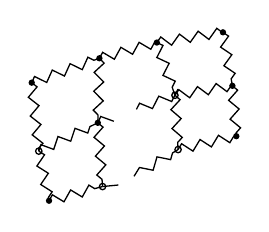
\begin{tikzpicture}[x=.010cm,y=-.010cm,line width=.47pt]
\coordinate (a) at (19,85);
\coordinate (b) at (105,54);
\coordinate (c) at (178,34);
\coordinate (d) at (262,21);
\coordinate (e) at (28,172);
\coordinate (f) at (103,136);
\coordinate (g) at (201,101);
\coordinate (h) at (274,89);
\coordinate (i) at (41,235);
\coordinate (j) at (109,217);
\coordinate (k) at (205,170);
\coordinate (l) at (279,153);
\foreach \from/\to in {a/b,b/c,c/d,a/e,b/f,c/g,d/h,e/f,g/h,e/i,f/j,g/k,h/l,i/j,k/l} {
  \draw[decorate,decoration={zigzag,amplitude=.62mm,segment length=2.4mm}] (\from)--(\to);
}
\draw[decorate,decoration={zigzag,amplitude=.60mm,segment length=2.6mm}]
  (f)--(127,126) (152,119)--(g) (j)--(128,209) (149,204)--(k);
\foreach \point in {a,b,c,d,f,h,i,l} \fill (\point) circle (1.15pt);
\foreach \point in {e,g,j,k} \draw (\point) circle (1.15pt);
\end{tikzpicture}}\endgroup\par
Места разрывов в середине и в нижнем ряду сохранены; точное соединение неясно.}
\end{GelfandAdjacentEvidence}
\begin{GelfandAdjacentEvidence}{GELFAND-P001045}{9}

Соединяем точки пружинками.

\uwave{Регул. решётка} не годится:
\SourceFigure{GELFAND-P001045}{surface-outline}{%
\begingroup\color{black}\GelfandFitDiagram{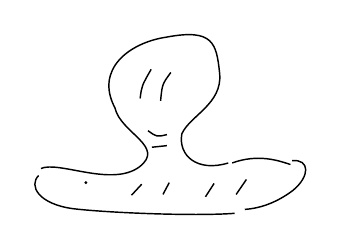
\begin{tikzpicture}[x=.010cm,y=-.010cm,line width=.52pt]
\draw (25,184) .. controls (48,174) and (115,208) .. (150,182)
 .. controls (184,156) and (126,139) .. (119,107)
 .. controls (93,58) and (137,24) .. (185,17)
 .. controls (244,6) and (248,25) .. (252,63)
 .. controls (256,102) and (214,117) .. (204,140)
 .. controls (199,168) and (224,189) .. (263,177);
\draw (268,177) .. controls (301,165) and (327,174) .. (342,179);
\draw (344,174) .. controls (367,172) and (367,194) .. (345,212)
 .. controls (321,230) and (299,235) .. (284,236);
\draw (271,241) .. controls (218,245) and (105,240) .. (65,235)
 .. controls (22,229) and (9,206) .. (22,193);
\draw (151,95)..controls (153,79)..(165,58);
\draw (177,98)..controls (179,77)..(190,62);
\draw (161,136)..controls (172,144)..(185,141);
\draw (166,157)--(185,155);
\draw (140,218)--(153,204) (180,217)--(188,202)
      (234,220)--(245,203) (273,217)--(286,198);
\fill (82,202) circle (.57pt);
\end{tikzpicture}}\endgroup\par
Сохраняются видимые разрывы; точное замыкание контура неясно.}
\end{GelfandAdjacentEvidence}


Для решётки:
\begin{equation*}
\int\mathcal{D}\vec{x}(\xi^1,\xi^2)
e^{-\frac12\int\partial_a\vec{x}\cdot\partial^a\vec{x}\,d^2\xi}
\tag{26}
\end{equation*}
(для 2-мерн. пов. в 26-мерном пр-ве получ. прав. ответ)

Пусть есть внутр. геом., опис. $g_{ab}(\xi)$. Интеграл примет вид:


\Needspace{7\baselineskip}
\begin{GelfandAdjacentEvidence}{GELFAND-P001046}{1}
\SourcePage{GELFAND-P001046}{13}
\begin{equation*}
G=\int\mathcal D\vec{x}(\xi)
\exp\left\{-\frac12\int\sqrt{g}\,g^{ab}\partial_a\vec{x}\cdot\partial_b\vec{x}\,d^2\xi
+\lambda\int\sqrt{g}\,d^2\xi\right\}
\tag{27}
\end{equation*}
с добавлением $\lambda$, к-рый мы подберём.

Ответ (правильный):
\begin{equation*}
\begin{aligned}
G={}&\int\mathcal Dg_{ab}\int\mathcal D\vec{x}(\xi)\\
&\times\exp\left\{-\frac12\int\sqrt{g}\,g^{ab}\partial_a\vec{x}\,\partial_b\vec{x}\,d^2\xi
+\lambda\int\sqrt{g}\,d^2\xi\right\}
\end{aligned}
\tag{28}
\end{equation*}
\SourceFigure{GELFAND-P001046}{kinetic-dot}{В (27) между производными стоит точка; в (28) её нет.}
\end{GelfandAdjacentEvidence}
\begin{GelfandAdjacentEvidence}{GELFAND-P001046}{2}


Минимизируя, получаем ур. я.

\medskip
\underline{4/$\overline{\underline{\mathrm{X}}}$-82 г.}\quad\underline{Сем. Гельфанда.}

\underline{\uuline{Кириллов} о раб. Гинзбурга}.

$G$ — группа Ли, $\mathfrak g$ — алгебра Ли, рассм. орбиты присоед. представления;

есть орбиты общего положения, есть нильпотентные (соотв. нильпот. элем. алгебры $\mathfrak g$);

$\Omega_c$ — орбита, $c=(c_1,\ldots,c_\ell)$ — её параметры ($\ell$ — ранг).

\underline{Пример}: $SL(2,\mathbb R)$; $\mathfrak g\cong\mathbb R^3$; орбиты — \uwave{гиперболоиды}.
\SourceFigure{GELFAND-P001046}{orbit-margin}{%
[На правом поле \(\Vert\)] напр., соб. знач. или,
\(\operatorname{Tr}A\), \(\operatorname{Tr}A^2,\ldots\)}
\end{GelfandAdjacentEvidence}
\begin{GelfandAdjacentEvidence}{GELFAND-P001046}{3}


\uwave{Десингуляризация по Спрингеру}.

$G$ — полупр. группа, $N\subset G$, $N$ — мн-во унипотентных элементов
(со всеми соб. знач. $1$).

$N$ — алгебр. мн-во с особ..
\Unclear{GELFAND-P001046}{cancelled-before-osob}{Перед «особ.» густо зачёркнута короткая запись; возможно, «о».}
\end{GelfandAdjacentEvidence}
\begin{GelfandAdjacentEvidence}{GELFAND-P001046}{4}


$B_0$ — борелевская подгр. в $G$; $\mathcal B$ — совок. всех борелевских подгрупп
(все они сопряжены), так что
\[
\mathcal B=\{gBg^{-1},\ g\in G\}.
\]
\SourceFigure{GELFAND-P001046}{borel-base-notation}{В формуле \(B\) без индекса, выше \(B_0\).}
\end{GelfandAdjacentEvidence}
\begin{GelfandAdjacentEvidence}{GELFAND-P001046}{5}


Десингуляризация алг. мн-зия $X$ (с особ.) — мн-зие $Y$ (без особ.)
той же размерности, $Y\longrightarrow X$ почти всюду вз. однозн.
(кроме меньшей разм.).
\Unclear{GELFAND-P001046}{cancelled-definition-start}{Перед «Десингуляризация» зачёркнуто слово, возможно «Всп.».}
\end{GelfandAdjacentEvidence}
\begin{GelfandAdjacentEvidence}{GELFAND-P001046}{6}

\Unclear{GELFAND-P001046}{overwritten-toi}{Слово «той» написано поверх исправления; прежние штрихи неразборчивы.}
\end{GelfandAdjacentEvidence}
\begin{GelfandAdjacentEvidence}{GELFAND-P001046}{7}


\underline{Пример}:
\SourceFigure{GELFAND-P001046}{cylinder-cone}{%
\begingroup\color{black}\GelfandFitDiagram{\begin{tikzpicture}[font=\scriptsize,line width=.55pt]
\draw (.20,.74) ellipse (.34 and .105);
\draw (-.14,.74)--(-.43,-.28) (.54,.74)--(.24,-.28);
\draw (-.28,.22) arc[start angle=180,end angle=360,x radius=.34,y radius=.10];
\draw[dashed] (-.28,.22) arc[start angle=180,end angle=0,x radius=.34,y radius=.10];
\draw (-.43,-.28) arc[start angle=180,end angle=360,x radius=.34,y radius=.11];
\draw[dashed] (-.43,-.28) arc[start angle=180,end angle=0,x radius=.34,y radius=.11];
\node at (.02,-.76) {цилиндр};
\draw[->] (.73,.23)--(1.58,.23);
\draw (2.25,.73) ellipse (.35 and .10);
\draw (1.90,.73)--(2.12,.15)--(1.67,-.45) (2.60,.73)--(2.12,.15)--(2.33,-.57);
\fill (2.12,.15) circle (.82pt);
\draw (1.67,-.45) .. controls (1.89,-.64) and (2.09,-.67) .. (2.33,-.57);
\draw[dashed] (1.76,-.42)--(2.05,-.47)--(2.23,-.50);
\node at (2.03,-.89) {конус.};
\end{tikzpicture}}\endgroup}
\end{GelfandAdjacentEvidence}
\begin{GelfandAdjacentEvidence}{GELFAND-P001046}{8}

\[
(x,y,z)\longmapsto(xz,yz,z).
\]

\Unclear{GELFAND-P001046}{cancelled-incidence-name}{После \(\mathcal M\) зачёркнуто неразборчивое обозначение.}
\end{GelfandAdjacentEvidence}
\begin{GelfandAdjacentEvidence}{GELFAND-P001046}{9}

\[
\mathcal M=\left\{\left(
\overset{\substack{N\\\rotatebox{-90}{\(\ni\)}}}{n},\,
\overset{\substack{\mathcal B\\\rotatebox{-90}{\(\ni\)}}}{B}
\right)\,\middle|\, n\in B\right\}\qquad\text{(флаги).}
\]
\SourceFigure{GELFAND-P001046}{incidence-membership}{Знаки принадлежности над \(n\) и \(B\) записаны вертикально.}
\end{GelfandAdjacentEvidence}
\begin{GelfandAdjacentEvidence}{GELFAND-P001046}{10}

Тогда $\mathcal M$ — десингуляризация $N$.
\Unclear{GELFAND-P001046}{cancelled-before-m}{После «Тогда» зачёркнуто обозначение; оно не читается.}
\end{GelfandAdjacentEvidence}
\begin{GelfandAdjacentEvidence}{GELFAND-P001046}{11}


Для $SL(2,\mathbb R)$ это как раз то, что в примере.

\underline{Снова о Гинзбурге}.
\[
f\in C^\infty(\mathfrak g)\longmapsto\psi(c)=\int_{\Omega_c}f
\]
(мера выб. на орбитах общего полож. согласованно).
\[
\int_{\Omega_0}f=\left.P\psi(c)\right|_{c=0},
\qquad P\text{ — дифф. оператор}
\]
\SourceFigure{GELFAND-P001046}{orbital-operator}{Оператор обозначен \(P\) в обоих местах.}
\end{GelfandAdjacentEvidence}



\Needspace{7\baselineskip}
\begin{GelfandAdjacentEvidence}{GELFAND-P001047}{1}
\SourcePage{GELFAND-P001047}{unlabelled}
\underline{И. М. Г.}\quad Даны интегралы по гиперболам. Найти значение ф-и в $0$.

(более общо — гиперболоид).

\SourceFigure{GELFAND-P001047}{hyperbola-sketch}{%
\begingroup\color{black}\GelfandFitDiagram{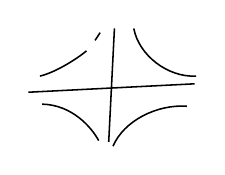
\begin{tikzpicture}[x=.91cm,y=.89cm,line width=.56pt]
\draw (-1.16,-.05)--(1.16,.07);
\draw (-.04,-.76)--(.04,.86);
\draw (-1.00,.18) .. controls (-.79,.23) and (-.49,.42) .. (-.35,.54);
\draw (-.23,.69)--(-.16,.80);
\draw (.31,.86) .. controls (.38,.48) and (.78,.16) .. (1.18,.18);
\draw (-.97,-.22) .. controls (-.55,-.23) and (-.28,-.55) .. (-.18,-.74);
\draw (.02,-.82) .. controls (.17,-.46) and (.63,-.22) .. (1.05,-.25);
\end{tikzpicture}}\endgroup\par
Короткий загиб у правого конца горизонтальной линии неясен.}
\end{GelfandAdjacentEvidence}
\begin{GelfandAdjacentEvidence}{GELFAND-P001047}{2}

\[
xy=c;\qquad\text{расст. от }0\text{ порядка }\sqrt c.
\]
При $|x|\geqslant1$ расст. $\sim c$.
\Unclear{GELFAND-P001047}{upper-inequality}{У знака \(>\) есть отдельный нижний косой штрих; вероятно, имеется в виду \(\geqslant\).}
\end{GelfandAdjacentEvidence}
\begin{GelfandAdjacentEvidence}{GELFAND-P001047}{3}


$\Rightarrow$ вычислим интегр. по прямым (предел инт. по гиперболам) и т. д.

См. разложение $\delta(xy-c)$ по степ. $c$ в 1-м вып. обобщ. ф-ий.

\medskip
\underline{Замолодчиков.}

Хотим найти сумму
\begin{equation*}
\sum_S e^{-\mu_0^2 A(S)}
\tag{1}
\end{equation*}
$S$ — поверхность

Интеграл по мн-ву всех кривых (см. выше) имел вид
\begin{equation*}
\begin{aligned}
\sum_P e^{-m_0L(P)}
&=\int_0^\infty d\tau\,e^{-m^2\tau}
\int_{\substack{\vec x(0)=\vec 0\\\vec x(\tau)=\vec R}}
\mathcal D\vec x(t)\,e^{-\frac12\int_0^\tau\dot{\vec x}^{\,2}(t)\,dt},\\
&\hspace{2em}L=\int\sqrt{\dot x^{2}}\,dt.
\end{aligned}
\tag{2}
\end{equation*}
\SourceFigure{GELFAND-P001047}{eq2-left-mass}{Между \(m\) и \(L\) виден нижний нуль, прилегающий к штриху \(L\).}
\end{GelfandAdjacentEvidence}
\begin{GelfandAdjacentEvidence}{GELFAND-P001047}{4}

\SourceFigure{GELFAND-P001047}{length-notation}{В формуле для \(L\) у \(\dot x\) нет стрелки.}
\end{GelfandAdjacentEvidence}
\begin{GelfandAdjacentEvidence}{GELFAND-P001047}{5}


($m\ne m_0$ — перенормировка)

И он равен:
\begin{equation*}
(\mathrm{const})\int_0^\infty d\tau
\left(e^{-m^2\tau-\frac{\vec R^{2}}{2\tau}}\right)\frac1{\tau^{d/2}},
\qquad d\text{ — размерность пр-ва}.
\tag{2'}
\end{equation*}
Связь $m$ и $m_0$ зависит от способа регуляризации [аппрок. — тонкой структ. пр-ва].

\begin{equation*}
\sum_P e^{-m_0L}=
\underset{\text{(интеграл)}}{\sum_{L=0}^{\infty}} f(L)e^{-m_0L}
\tag{3}
\end{equation*}
где
\[
f(L)\sim L^\beta e^{\varkappa L}
\qquad\text{при }L\gg\varepsilon
\qquad(\varepsilon\text{ — шаг решётки})
\]
\[
\varkappa=\varkappa(\varepsilon),\qquad\beta\text{ не зависит от }\varepsilon.
\]
\Unclear{GELFAND-P001047}{growth-parameter}{Петлеобразный знак передан как \(\varkappa\); возможно, рукописное \(x\).}
\end{GelfandAdjacentEvidence}
\begin{GelfandAdjacentEvidence}{GELFAND-P001047}{6}


Отсюда
\begin{equation*}
(3)=\mathrm{const}\sum(L)^\beta e^{-(m_0-\varkappa)L}
\tag{4}
\end{equation*}
\[
m^2=m_0-\varkappa.
\]

\uwave{2 опасности}:

а) сосред. на прямых

б) расходится

\SourceFigure{GELFAND-P001047}{risk-first-margin}{%
[Справа от обоих пунктов \(\Vert\)] обходятся выбором \(m_0\).}
\end{GelfandAdjacentEvidence}
\begin{GelfandAdjacentEvidence}{GELFAND-P001047}{7}

\SourceFigure{GELFAND-P001047}{risk-second-margin}{%
[Ещё правее \(\Vert\)] В \(\infty\)-мерном пр-ве почти \(\forall\) две меры взаимно сингулярны.}
\end{GelfandAdjacentEvidence}



\Needspace{7\baselineskip}
\begin{GelfandAdjacentEvidence}{GELFAND-P001048}{1}
\SourcePage{GELFAND-P001048}{14}
\uwave{Перейдём к поверхностям}.

$\vec{x}(\xi^1,\xi^2)$;\quad $g_{ab}(\xi^1,\xi^2)$ — метрика на пов..

\begin{equation*}
\begin{aligned}
\sum_S e^{-\mu_0^2 A(S)}
={}&\int d\mu(\vec{x},g)\exp\Bigl\{-\frac12\int\sqrt{g}\,g^{ab}
\partial_a\vec{x}\,\partial_b\vec{x}\,d^2\xi{}-\\
&\qquad{}-\mu_{0}^{2}\int\sqrt{g}\,d^2\xi\Bigr\},
\qquad g=\det g_{ab}.
\end{aligned}
\tag{5}
\end{equation*}
\Unclear{GELFAND-P001048}{eq5-mu-subscript}{Нижний индекс у второго \(\mu\) сильно обведён; вероятно, \(0\).}
\end{GelfandAdjacentEvidence}
\begin{GelfandAdjacentEvidence}{GELFAND-P001048}{2}


(ф-ла Полякова) Здесь суммир. по поверхн. [вписано сверху: с] зад. топ. св-вами.
\SourceFigure{GELFAND-P001048}{top-preposition-insertion}{«с» вписано между «поверхн.» и «зад.».}
\end{GelfandAdjacentEvidence}
\begin{GelfandAdjacentEvidence}{GELFAND-P001048}{3}


\[
\left[
\begin{minipage}{.87\linewidth}
Вообще-то Надо учитывать пов. с ручками и дырками.

Неясно, каково соотн. вкладов.\quad Надо: $\displaystyle\sum$, $j$ — число ручек.

Пенистые пов. (с большим числом ручек) могут вносить подавляющий вклад.
\end{minipage}
\right.
\]
\Unclear{GELFAND-P001048}{handles-sum-index}{Под \(\sum\) виден малый штрих; индекс \(j\) там неразличим. Справа \(j\) назван числом ручек.}
\end{GelfandAdjacentEvidence}
\begin{GelfandAdjacentEvidence}{GELFAND-P001048}{4}


Здесь выбир. область параметров в $\mathbb R^2$.
Вводятся [вписано сверху: элементы] расстояния в функц. пр-ве:
\SourceFigure{GELFAND-P001048}{distance-verb}{Начало фразы читается как «Вводятся».}
\end{GelfandAdjacentEvidence}
\begin{GelfandAdjacentEvidence}{GELFAND-P001048}{5}

\SourceFigure{GELFAND-P001048}{distance-insertion}{Над строкой написано «элементы».}
\end{GelfandAdjacentEvidence}
\begin{GelfandAdjacentEvidence}{GELFAND-P001048}{6}

\SourceFigure{GELFAND-P001048}{distance-noun}{На строке написано «расстояния».}
\end{GelfandAdjacentEvidence}
\begin{GelfandAdjacentEvidence}{GELFAND-P001048}{7}

\begin{equation*}
\begin{aligned}
\|\delta\vec{x}(\xi^1,\xi^2)\|^2
&=\int\sqrt{g}\,(\delta\vec{x}(\xi))^2\,d^2\xi\\
\|\delta g\|^2
&=\int\sqrt{g}\,
\bigl(g^{aa'}g^{bb'}+c\,g^{ab}g^{a'b'}\bigr)
\delta g_{ab}\,\delta g_{a'b'}\,d^2\xi
\end{aligned}
\tag{6}
\end{equation*}
Калибр. инвариантность: при преобр.:
\begin{equation*}
\begin{cases}
\xi^a\to\xi^a+\varepsilon^a(\xi),\\
g_{ab}\to g_{ab}+\nabla_a\varepsilon_b+\nabla_b\varepsilon_a,
\end{cases}
\qquad
\nabla_a\varepsilon_b=\partial_a\varepsilon_b+\Gamma_{ab}^{c}\varepsilon_c.
\tag{7}
\end{equation*}
ничего не меняется.
\SourceFigure{GELFAND-P001048}{covariant-derivative-sign}{Перед \(\Gamma_{ab}^{c}\) в (7) стоит знак \(+\).}
\end{GelfandAdjacentEvidence}
\begin{GelfandAdjacentEvidence}{GELFAND-P001048}{8}


Надо интегр. по \uuline{пр-ву орбит}.
\begin{equation*}
d\mu(x,g)=\frac{\mathcal{D}\vec{x}\,\mathcal{D}g}{\mathcal{D}\omega}
\tag{8}
\end{equation*}
\begin{equation*}
\|\varepsilon\|^2=\int\sqrt{g}\,g^{ab}\varepsilon_a\varepsilon_b\,d^2\xi
\tag{9}
\end{equation*}
\SourceFigure{GELFAND-P001048}{measure-margin}{%
[Справа от (8) и (9)] \(\mathcal D\omega\) — мера в группе, по к-рой факториз.,\\
\(\mathcal D\vec{x}\) и \(\mathcal D g\) ввод. по метрикам \underline{(6)}\\
\(\mathcal D\omega\) — по метрике (9) на алгебре Ли.}
\end{GelfandAdjacentEvidence}
\begin{GelfandAdjacentEvidence}{GELFAND-P001048}{9}


Теперь интеграл [вписано сверху: (5)] определён хорошо.
\SourceFigure{GELFAND-P001048}{eq5-number-insertion}{Ссылка «(5)» вписана над строкой.}
\end{GelfandAdjacentEvidence}
\begin{GelfandAdjacentEvidence}{GELFAND-P001048}{10}


$\int\mathcal{D}\vec{x}$ гауссов — сводится к $\underline{\det}$ оператора.

Поляков предлагает выбрать представителей так:
\begin{equation*}
g_{ab}=\delta_{ab}\,\rho(\xi^1,\xi^2)
\qquad\text{(конформно плоский вид).}
\tag{10}
\end{equation*}
(выбор калибровки). Остаётся конформная группа (конечномерная).
\SourceFigure{GELFAND-P001048}{conformal-group-adjective}{Начальные штрихи «конечномерная» переписаны.}
\end{GelfandAdjacentEvidence}


$\det$ одинаковы. Получается
\begin{equation*}
\int d\mu(\rho)\,[\det(\Delta_g)]^{(26-d)/2},
\qquad\Delta_g\text{ — лапласиан метрики}
\tag{11}
\end{equation*}
($\rho$ — коэфф. в (10)).


\Needspace{7\baselineskip}
\begin{GelfandAdjacentEvidence}{GELFAND-P001049}{1}
\SourcePage{GELFAND-P001049}{unlabelled}
Получается:
\begin{equation*}
(11)=\int d\mu(\varphi)\,
e^{\frac{d-26}{48\pi}\int\frac12(\partial_a\varphi)^2+
m^{2}e^{\varphi})\,d^2\xi}
\tag{12}
\end{equation*}
\SourceFigure{GELFAND-P001049}{eq11-crossreference}{Слева от знака равенства обведено «(11)».}
\end{GelfandAdjacentEvidence}
\begin{GelfandAdjacentEvidence}{GELFAND-P001049}{2}

\Unclear{GELFAND-P001049}{eq12-mass-symbol}{Основание степени перед \(e^\varphi\) густо обведено и читается как \(m\). Прежние штрихи неразборчивы.}
\end{GelfandAdjacentEvidence}
\begin{GelfandAdjacentEvidence}{GELFAND-P001049}{3}

\Unclear{GELFAND-P001049}{eq12-parentheses}{После \(e^\varphi\) стоит закрывающая скобка. Открывающая скобка для всей суммы не видна.}
\end{GelfandAdjacentEvidence}


$d\mu(\varphi)$ — мера из метрики
\begin{equation*}
\|\delta\varphi\|^2=\int e^{\varphi}(\delta\varphi)^2\,d^2\xi
\tag{13}
\end{equation*}


\Needspace{7\baselineskip}
\begin{GelfandAdjacentEvidence}{GELFAND-P001050}{1}
\SourcePage{GELFAND-P001050}{unlabelled}
\underline{11/$\overline{\underline{\mathrm{X}}}$-82 г.}\qquad
\uwave{Сем. Гельфанда}

\uuline{В. Гинзбург.}

\underline{по Гийемину-Стернбергу} (об интегр. геом.)
\SourceFigure{GELFAND-P001050}{guillemin-sternberg-heading}{В правой части заголовка: «по Гийемину-Стернбергу».}
\end{GelfandAdjacentEvidence}
\begin{GelfandAdjacentEvidence}{GELFAND-P001050}{2}


$X$ — мн-зие (комплексное)

$\Sigma\subset T^*X$, $\Sigma$ — коизотропное подмн-во,
\Unclear{GELFAND-P001050}{crossed-after-submanifold}{После «подмн-во» зачёркнуто слово, возможно «которое» или «коническое».}
\end{GelfandAdjacentEvidence}
\begin{GelfandAdjacentEvidence}{GELFAND-P001050}{3}

облад. след. св-вами:

1.\quad $\Sigma$ — коническое;

2.\quad $\Sigma\to X$ расслоение.

На $\Sigma$ имеется $0$-слоение (ядро симплект. формы), к-рое всегда \uwave{интегрируемо}.

Локально устр. так: $q_1,\ldots,q_n,p_1,\ldots,p_k$

$0$-слоение
\SourceFigure{GELFAND-P001050}{null-foliation-bracket}{%
\begingroup\color{black}\GelfandFitDiagram{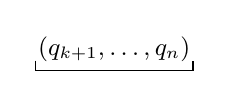
\begin{tikzpicture}[font=\small,line width=.45pt]
\node (coords) at (0,0) {$(q_{k+1},\ldots,q_n)$};
\draw (coords.south west) ++(.09,.14) -- ++(0,-.13)
  -- ([xshift=-.09cm,yshift=.01cm]coords.south east) -- ++(0,.13);
\end{tikzpicture}}\endgroup}
\end{GelfandAdjacentEvidence}
\begin{GelfandAdjacentEvidence}{GELFAND-P001050}{4}


\Unclear{GELFAND-P001050}{mark-before-pust}{Перед «Пусть» помета с несколькими штрихами. Возможно, «Мы» или «Или».}
\end{GelfandAdjacentEvidence}
\begin{GelfandAdjacentEvidence}{GELFAND-P001050}{5}

Пусть оно является \uwave{расслоением} (все слои замкнуты и т.п.)
\SourceFigure{GELFAND-P001050}{quotient-arrow}{%
\begingroup\color{black}\GelfandFitDiagram{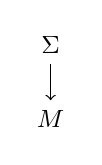
\begin{tikzpicture}[font=\small,line width=.47pt]
\node (from) at (0,.45) {$\Sigma$};
\node (to) at (0,-.48) {$M$};
\draw[->] (from.south)--(to.north);
\end{tikzpicture}}\endgroup}
\end{GelfandAdjacentEvidence}

и $M$ — факторпр-во.

По $\Sigma$ построим лагранжево подмн-зие $\Lambda\subset T^*X\times T^*X$:
\[
\Lambda=\{(\xi_1,\xi_2):\quad\xi_1,\xi_2\in\Sigma,\quad\xi_1\sim\xi_2\}
\]
\underline{Св-ва}:

1)\quad $\Lambda^t=\Lambda$

2)\quad $\Lambda\circ\Lambda=\Lambda$ \qquad (проектор)


\Needspace{7\baselineskip}
\begin{GelfandAdjacentEvidence}{GELFAND-P001051}{1}
\SourcePage{GELFAND-P001051}{unlabelled}
По-видимому, обратно: если $\Lambda$ лагранжево и вып. 1), 2), то оно получается из $\Sigma$.
\Unclear{GELFAND-P001051}{top-cancel-01}{После «и» густо зачёркнуто слово; под зачёркиванием видна петля.}
\end{GelfandAdjacentEvidence}
\begin{GelfandAdjacentEvidence}{GELFAND-P001051}{2}


Интегральные опер. Фурье строятся по $\Lambda$: обозн. их мн-во $\mathcal E_\Lambda$.

Оно кольцо в силу св-ва 2).
\Unclear{GELFAND-P001051}{top-cancel-02}{Перед «св-ва» зачёркнута короткая запись.}
\end{GelfandAdjacentEvidence}
\begin{GelfandAdjacentEvidence}{GELFAND-P001051}{3}


Это аналог преобр. Радона.

$X=X_1\times X_2$;\quad $\Sigma$ — направл., нормальные к $X_1$ (вдоль $X_2$)
в кокас. рассл.
\[
\begin{aligned}
\Lambda
&=\operatorname{diag}(T^*X_1\times T^*X_1)\times 0\\
&\subset T^*X_1\times T^*X_1\times T^*X_2\times T^*X_2.
\end{aligned}
\]
\Unclear{GELFAND-P001051}{lambda-cancel}{Перед \(\operatorname{diag}\) зачёркнута формула; различимы отдельные знаки, похожие на \(T^*\), \(X_1\), \(\times\), \(0\).}
\end{GelfandAdjacentEvidence}
\begin{GelfandAdjacentEvidence}{GELFAND-P001051}{4}


\dashuline{Операторы}:\quad по $X_1$ все псевдодифф.

\hspace{5em}по $X_2$ сглаживающие.

\uuline{Шмелёв.}
\SourceFigure{GELFAND-P001051}{speaker-name}{Дважды подчёркнутая фамилия читается «Шмелёв».}
\end{GelfandAdjacentEvidence}
\begin{GelfandAdjacentEvidence}{GELFAND-P001051}{5}

\SourceFigure{GELFAND-P001051}{double-fibration}{%
\begingroup\color{black}\GelfandFitDiagram{\begin{tikzpicture}[font=\small,line width=.50pt]
\node (z) at (0,.49) {$Z$};
\node (x) at (-.80,-.51) {$X$};
\node (y) at (.82,-.51) {$Y$};
\draw[->] (z.south west)--node[left,inner sep=1pt] {$\psi_1$} (x.north east);
\draw[->] (z.south east)--node[right,inner sep=1pt] {$\psi_2$} (y.north west);
\node[anchor=west,font=\scriptsize] at (1.32,.11) {расслоения};
\end{tikzpicture}}\endgroup}
\end{GelfandAdjacentEvidence}
\begin{GelfandAdjacentEvidence}{GELFAND-P001051}{6}


Требование:\quad
\uwave{\(\psi_2^*:N^*Z\longrightarrow T^*Y\)}
\quad вложение;

\underline{Фрёлих}

1) Магн. монополи

2) Калибр. теории\quad $G\overset{\text{напр.}}{=}SU(2)$

Лагранжиан:\quad $\varphi:\ \mathrm{isospin}=1$ \quad (3-комп.)
\begin{equation*}
\begin{aligned}
E
&=\int\{(D_A\varphi)^2+F^2\}\\
&=\int\Bigl\{
\bigl|(\partial_\mu-eA_\mu\wedge)\varphi(x)\bigr|^2
+\operatorname{tr}(F_{\mu\nu}\cdot F^{\mu\nu})(x)
\Bigr\}\,dx,
\end{aligned}
\tag{1}
\end{equation*}
\SourceFigure{GELFAND-P001051}{energy-wedge}{После \(A_\mu\) стоит знак, похожий на \(\wedge\).}
\end{GelfandAdjacentEvidence}
\begin{GelfandAdjacentEvidence}{GELFAND-P001051}{7}

\Unclear{GELFAND-P001051}{energy-norm-cancel}{Под степенью \(2\) у нормы густо зачёркнуто обозначение.}
\end{GelfandAdjacentEvidence}
\begin{GelfandAdjacentEvidence}{GELFAND-P001051}{8}

\Unclear{GELFAND-P001051}{energy-trace-cancel}{Под точкой между двумя \(F\) видны переписанные штрихи и извилистая линия. Первоначальные знаки не установлены.}
\end{GelfandAdjacentEvidence}
\begin{GelfandAdjacentEvidence}{GELFAND-P001051}{9}


$x\in\mathbb R^3$
\Unclear{GELFAND-P001051}{energy-line-cancel}{Справа от \(x\in\mathbb R^3\) зачёркнуто равенство; начало похоже на \(E=E\).}
\end{GelfandAdjacentEvidence}
\begin{GelfandAdjacentEvidence}{GELFAND-P001051}{10}

\[
F_{\mu\nu}=\partial_\mu A_\nu-\partial_\nu A_\mu+[A_\mu,A_\nu].
\]

Монополь:\quad такое реш. ур-й Эйлера-Лагр., что степень $\varphi|_{S^2}\longrightarrow S^2$
на \(\infty\) равна 1.\quad \(\Vert\) (стац. решения)

$\exists$ реш., реализу. $\min$ или $\text{лок.}\,\min$ — явно, используя твисторную техн.
\Unclear{GELFAND-P001051}{twistor-cancel}{Перед «твисторную» зачёркнута короткая запись.}
\end{GelfandAdjacentEvidence}
\begin{GelfandAdjacentEvidence}{GELFAND-P001051}{11}


Вопрос:\quad другие стац. точки?

\uwave{Ответ}:\quad найдены реш., не явл. минимумами

\underline{Идея}:
\SourceFigure{GELFAND-P001051}{lower-loop-diagram}{%
\begingroup\color{black}\GelfandFitDiagram{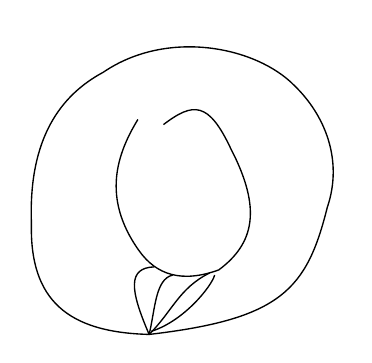
\begin{tikzpicture}[x=.013cm,y=-.013cm,line width=.49pt]
\draw (123,307) .. controls (44,305) and (6,274) .. (8,198)
 .. controls (5,115) and (37,73) .. (78,51)
 .. controls (141,8) and (228,26) .. (265,64)
 .. controls (294,92) and (313,136) .. (297,183)
 .. controls (277,263) and (252,292) .. (123,307);
\draw (137,102) .. controls (166,80) and (181,79) .. (203,126)
 .. controls (233,184) and (226,218) .. (191,244)
 .. controls (155,257) and (130,249) .. (113,225)
 .. controls (76,173) and (92,130) .. (112,97);
\draw (123,307) .. controls (104,263) and (102,242) .. (128,241);
\draw (123,307) .. controls (129,282) and (129,253) .. (146,249);
\draw (123,307) .. controls (146,284) and (152,262) .. (182,247);
\draw (125,304) .. controls (157,294) and (184,260) .. (187,249);
\end{tikzpicture}}\endgroup\par
У внутренней петли виден разрыв. Точное соединение тонких линий у нижней точки неразличимо.}
\end{GelfandAdjacentEvidence}
\begin{GelfandAdjacentEvidence}{GELFAND-P001051}{12}


однопар. сем-во:
\[
\max_{[\rho?]\,t\in\mathrm{curve}}\ \min_{\mathrm{curve.}}(\varphi_t,F_t)
\]
\Unclear{GELFAND-P001051}{minimax-index}{Перед \(t\in\mathrm{curve}\) знак, похожий на \(\rho\) или \(p\). Под \(\min\) написано «curve.».}
\end{GelfandAdjacentEvidence}


C. Taubes

Новое реш. похоже на пару

монополь / антимонополь.


\Needspace{7\baselineskip}
\begin{GelfandAdjacentEvidence}{GELFAND-P001052}{1}
\SourcePage{GELFAND-P001052}{16}
\uwave{Имеется мн-зие}\quad
$\underset{\text{(компактное)}}{M^4}$,
$\pi_1(M^4)=\{\mathrm{id}\}$;
$H^2(M^4)=\{0\}$.

$M^4$ с конформной структ..

$\exists\, [A_\mu?]$ реш. ур-я $F=\pm F^*$?
\Unclear{GELFAND-P001052}{top-field-symbol}{Начальный знак после \(\exists\) переписан, возможно \(A_\mu\).}
\end{GelfandAdjacentEvidence}
\begin{GelfandAdjacentEvidence}{GELFAND-P001052}{2}


$*$ — двойств. по Ходжу;

с хар. классом 1 — \uwave{[напр.?]}
\Unclear{GELFAND-P001052}{top-underlined-name}{Подчёркнутое слово после «классом 1» читается предположительно как «напр.». Начало переписано.}
\end{GelfandAdjacentEvidence}
\begin{GelfandAdjacentEvidence}{GELFAND-P001052}{3}


$F$ кривизна связности $A$; гр. — $SU(2)$.

Ответ:\quad реш. существует!

Пр-во параметров, метящих решения
$\displaystyle=\underset{\substack{\nwarrow\\\text{мн-зие }B}}{5}$
\qquad (как на сфере!)

(Taubes, Comm. Math. Phys, 1981).

Парам. инстантона

$B$ — мн-зие с краем,
$\displaystyle\partial B\underset{\substack{\uparrow\\\text{\uwave{Donaldson}}}}{\simeq}M^4$
\quad (исх. мн-зие)
\SourceFigure{GELFAND-P001052}{boundary-annotation}{Слово «Donaldson» соединено ломаной стрелкой со знаком \(\simeq\).}
\end{GelfandAdjacentEvidence}
\begin{GelfandAdjacentEvidence}{GELFAND-P001052}{4}


\begin{align*}
M^4\text{ — край}
&\Longleftrightarrow(\text{понтр. }\text{[?]}\ \text{класс}=0)\\
&\Longleftrightarrow(\text{сигнатура}=0\text{ для формы в }H^2).
\end{align*}
\Unclear{GELFAND-P001052}{pontryagin-symbol}{Между «понтр.» и «класс» густо обведён знак. Возможно, \(p\).}
\end{GelfandAdjacentEvidence}
\begin{GelfandAdjacentEvidence}{GELFAND-P001052}{5}


\uwave{Donaldson}: если форма на $H^2$ положит. опред., то мн-зие $=$
обобщ. проект. плоск. $CP^2$
$\Rightarrow$ форма прив. к сумме квадратов (над $\mathbb Z$).
\Unclear{GELFAND-P001052}{definite-cancel}{Между «положит.» и «опред.» короткая зачёркнутая запись.}
\end{GelfandAdjacentEvidence}
\begin{GelfandAdjacentEvidence}{GELFAND-P001052}{6}

\Unclear{GELFAND-P001052}{manifold-cancel}{Слово сразу после знака равенства зачёркнуто.}
\end{GelfandAdjacentEvidence}
\begin{GelfandAdjacentEvidence}{GELFAND-P001052}{7}

\Unclear{GELFAND-P001052}{projective-correction}{После «проект.» зачёркнута запись. «плоск.» вписано сверху, а \(CP^2\) снизу; оба дополнения обведены.}
\end{GelfandAdjacentEvidence}
\begin{GelfandAdjacentEvidence}{GELFAND-P001052}{8}


$B$ должно иметь особ. — конусы над $CP^2$.

\underline{О раб.} \uwave{Witten’а}.

$M$ — $n$-мерное мн-зие, $B_p$ — \(p\)-е число Бетти.

$f$ — ф-я на $M$ с изол. крит. точками.

$M_p$ — число крит. точек с индексом $p$ (гессиан имеет $p$ отриц. соб. знач.).
\[
M_p\geqslant B_p
\qquad\underset{\text{простейшее}}{\text{(нер-во Морса)}}
\]

$d:\Omega_p\longrightarrow\Omega_{p+1}$ (внешн. дифф.)
\Unclear{GELFAND-P001052}{differential-cancel}{Перед скобкой «внешн. дифф.» зачёркнут знак.}
\end{GelfandAdjacentEvidence}
\begin{GelfandAdjacentEvidence}{GELFAND-P001052}{9}


Введ. метрику на $M$; $*$ — соотв. оператор.

Выб. в $H^p$ базис из гармонических $p$-форм ($B_p$ штук)

\uwave{Иначе}: положим
\[
d_t=e^{-tf}d\,e^{tf}
\]
\SourceFigure{GELFAND-P001052}{omega-exponent}{%
\begingroup\color{black}\GelfandFitDiagram{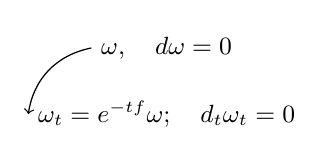
\begin{tikzpicture}[font=\small,line width=.45pt]
\node (top) at (0,.40) {$\omega,\quad d\omega=0$};
\node (bottom) at (0,-.44) {$\omega_t=e^{-tf}\omega;\quad d_t\omega_t=0$};
\draw[->] (top.west) to[bend right=35] (bottom.west);
\end{tikzpicture}}\endgroup\par
Показатель при \(e\) переписан и читается как \(-tf\).}
\end{GelfandAdjacentEvidence}
\begin{GelfandAdjacentEvidence}{GELFAND-P001052}{10}


Выб. базис в $H^p$, удовлетвор. условиям:
\begin{equation*}
\left\{
\begin{aligned}
-d_t\omega_j&=0\\
-(\omega_j,d_t\beta)&=0,\quad\forall\beta\in\Omega_{p-1}
\end{aligned}
\right\}
\ \Rightarrow\
(d_t^*d_t+d_t d_t^*)\omega_j=0
\tag{1}
\end{equation*}
\begin{flushright}(замкн. в новом смысле).\end{flushright}
\Unclear{GELFAND-P001052}{harmonic-first-stroke}{Короткий штрих перед \(d_t\omega_j\) может быть минусом или знаком перечисления.}
\end{GelfandAdjacentEvidence}
\begin{GelfandAdjacentEvidence}{GELFAND-P001052}{11}

\Unclear{GELFAND-P001052}{harmonic-second-stroke}{Перед второй строкой также стоит отдельный горизонтальный штрих.}
\end{GelfandAdjacentEvidence}



\Needspace{7\baselineskip}
\begin{GelfandAdjacentEvidence}{GELFAND-P001053}{1}
\SourcePage{GELFAND-P001053}{unlabelled}
$d_t$-когом. те же, что $d$-когом., т.к. есть \uwave{гомотопия}.
\[
d_t^2=0\quad\text{(очевидно)}
\]
Вычислим оператор $\Box_t=d_t^*d_t+d_td_t^*$ и найдём его асимпт.
при $t\to\infty$.
\SourceFigure{GELFAND-P001053}{operator-word}{Написано «Вычислим оператор». Внутри знака \(\Box\) виден косой штрих.}
\end{GelfandAdjacentEvidence}
\begin{GelfandAdjacentEvidence}{GELFAND-P001053}{2}

\begin{equation*}
\begin{cases}
d_t=d-tdf\cdot a^*,\\
d_t^*=d^*-tdf\cdot a
\end{cases}
\qquad
\begin{gathered}
df\,a^*\omega\equiv df\wedge\omega\\
\text{(физич. обознач.)}
\end{gathered}
\tag{2}
\end{equation*}
\SourceFigure{GELFAND-P001053}{eq2-sign-consistency}{Перед обоими членами \(tdf\) в (2) стоят минусы.}
\end{GelfandAdjacentEvidence}
\begin{GelfandAdjacentEvidence}{GELFAND-P001053}{3}

\begin{equation*}
\{a_j,a_i^*\}=\delta_{ij}.
\tag{3}
\end{equation*}
$a_i$ — \sout{базис} соотв. базису 1-форм;
(опер. внешнего умножения).
\SourceFigure{GELFAND-P001053}{basis-cancellation}{После \(a_i\) слово «базис» зачёркнуто.}
\end{GelfandAdjacentEvidence}
\begin{GelfandAdjacentEvidence}{GELFAND-P001053}{4}


Выбир. так, что выполнено (3).
\Unclear{GELFAND-P001053}{middle-operators}{Перед «выполнено» густо зачёркнута запись. Возможно, содержит \(a_i\).}
\end{GelfandAdjacentEvidence}
\begin{GelfandAdjacentEvidence}{GELFAND-P001053}{5}


\underline{Кириллов}:
\[
a=(a^1,a^2,\ldots,a^n)\text{ — \uwave{вектор}},\qquad
df=(\partial_1f,\partial_2f,\ldots,\partial_nf)
\]
$a^i$ — внутр. умножение (опер. уничтож.) — зачерк. $dx^i$, где есть,
где нет — аннулир..
\Unclear{GELFAND-P001053}{middle-cancellation}{Перед «уничтож.» зачёркнуто слово, возможно «рож.».}
\end{GelfandAdjacentEvidence}
\begin{GelfandAdjacentEvidence}{GELFAND-P001053}{6}


$a^{i*}$ — внешнее умножение.

Индексы можно опускать и поднимать с пом. метрики.

$a^j$ — внутр. умножение на $\dfrac{\partial}{\partial x^j}$ (подстан. в 1-й аргум.)

$df\cdot a$ — внутр. умн. на поле, получ. из $df$ поднятием индекса
\[
a_i^*=dx_i\wedge\qquad\text{(внешнее умн.)}
\]
\underline{Фрёлих.}
\[
a_i=\partial/\partial x_i\,
\tikz[baseline=0pt,x=1em,y=1em]{\draw (0,.62)--(0,0)--(.68,0);}
\qquad\text{(внутр. умн.)}
\]
\SourceFigure{GELFAND-P001053}{contraction-corner}{После \(\partial/\partial x_i\) написан угловой знак.}
\end{GelfandAdjacentEvidence}
\begin{GelfandAdjacentEvidence}{GELFAND-P001053}{7}

Смысл:

Одночастичное пр-во (фермионов)
\[
\{1,2,\ldots,n\}\to\ell_2(\{1,2,\ldots,n\}).
\]
($\ell_2$ на конечном мн-ве).
\[
m\text{ частиц (фермионов)}\Rightarrow f_{i_1\ldots i_m}
\]
(антисимм. $\delta$-ф-и — базис)

Способ записывать элем. грассм. ал.

(см. Березин: Метод втор. квант.)
\begin{equation*}
\sum_{i_1\ldots i_m}a_{i_1}^*\ldots a_{i_m}^*f_{i_1\ldots i_m}\Omega_0
\tag{4}
\end{equation*}
\[
\begin{gathered}
\updownarrow\\
(f_{i_1}\ldots f_{i_m})\quad\text{(набор коэфф.)}
\end{gathered}
\]
\Unclear{GELFAND-P001053}{lower-coefficients}{Последнее основание переписано; возможно, \(f_{i_m}\) или \(h_{i_m}\).}
\end{GelfandAdjacentEvidence}



\Needspace{7\baselineskip}
\begin{GelfandAdjacentEvidence}{GELFAND-P001054}{1}
\SourcePage{GELFAND-P001054}{17}
Постулируется:
\begin{equation*}
\{a_i,a_j^*\}=\delta_{ij}
\tag{5}
\end{equation*}
Внешн. умн. на $df$ — опер. рождения фермиона.
\begin{equation*}
a_i\Omega_0=0,\quad\forall i
\tag{6}
\end{equation*}
\begin{equation*}
\Box_t=\Box+t^2(df)^2+t\sum[a_i^*,a_j]\partial_i\partial_jf
\tag{7}
\end{equation*}
В окр. критич. точки
\begin{equation*}
f(x)=\sum_{i=1}^{n-p}\lambda_i(x^i-x_0^i)^2
-\sum_{j=n-p+1}^{n}\lambda_j(x^j-x_0^j)^2
+O(|x-x_0|^3)
\tag{8}
\end{equation*}
\begin{center}— . —\end{center}

\underline{И. М. Г.}\quad Идея: вместо перестроек в циклах — \uwave{перестройки в формах}!

Связь П.Д.О. и \dashuline{перестроек Морса}.

Ф.\quad\uwave{гл. член} $\Box_t$ \uwave{равен}:
\begin{equation*}
\Box+4t^2\sum_{j=1}^{n}\lambda_j^2(x^j-x_0^j)^2+
\overbrace{t\sum_{i<j}[a_i^*,a_j]\underset{\text{const}}{c_{ij}}}
\tag{9}
\end{equation*}
[Над последним членом]
\[
-4t\sum_{1}^{n-p}[a_i,a_i^*]\lambda_i
+4t\sum_{n-p+1}^{n}\lambda_i[\,].
\]
\SourceFigure{GELFAND-P001054}{expansion-above-nine}{Во второй сумме квадратные скобки пусты.}
\end{GelfandAdjacentEvidence}
\begin{GelfandAdjacentEvidence}{GELFAND-P001054}{2}

\Unclear{GELFAND-P001054}{middle-margin-cancellation}{Над скобкой зачёркнуто короткое слово, возможно «знак», далее две косые черты.}
\end{GelfandAdjacentEvidence}
\begin{GelfandAdjacentEvidence}{GELFAND-P001054}{3}

\SourceFigure{GELFAND-P001054}{eq9-summation-index}{Под суммой в (9) написано \(i<j\).}
\end{GelfandAdjacentEvidence}
\begin{GelfandAdjacentEvidence}{GELFAND-P001054}{4}

\begin{equation*}
\bigm|\ \approx\quad\text{\uwave{Аннулирует}}:\quad
\underline{dx_{n-p+1}\wedge\cdots\wedge dx_n}\quad(p\text{-форма})
\tag{10}
\end{equation*}
\SourceFigure{GELFAND-P001054}{annihilation-form}{Запись \(p\)-формы обведена нижней скобкой.}
\end{GelfandAdjacentEvidence}
\begin{GelfandAdjacentEvidence}{GELFAND-P001054}{5}

Посмотрим: не $0$-е, а малые соб. значения.
\SourceFigure{GELFAND-P001054}{eigenvalue-word}{В рукописи «малые соб. значения».}
\end{GelfandAdjacentEvidence}
\begin{GelfandAdjacentEvidence}{GELFAND-P001054}{6}


$\forall$ крит. точка даёт приближение к соб. ф-и.

2-й [вписано сверху: член]
компенсирует 1-й ровно на 1-м векторе (10).
\Unclear{GELFAND-P001054}{middle-second-term}{После «2-й» зачёркнуто слово, возможно «вектор», и вписано «член».}
\end{GelfandAdjacentEvidence}
\begin{GelfandAdjacentEvidence}{GELFAND-P001054}{7}


Компенсация — из сообр. суперсимметрии.

$d_t$ играет роль суперзаряда; модель Юкавы — компенсация известна.
\begin{equation*}
a=\frac{\delta}{\delta\varphi(x)}+ta^*(x)\varphi^n(x)
\leftrightarrow d+tdf\cdot a^*
\tag{11}
\end{equation*}
\SourceFigure{GELFAND-P001054}{eq11-field-power}{В (11) у \(\varphi\) виден показатель \(n\).}
\end{GelfandAdjacentEvidence}


\underline{$d=2$}$\Rightarrow$ фермионы $=$ формы на мн-ии конфигураций Бозе-полей.

(т.к. гр. Пуанкаре простая)

\underline{$d>2$}$\Rightarrow$ (?) нужны калибр. поля для интерпретации. —

— нет интерпретации (такой) пока.

\underline{V. Enss} — асимпт. полнота сист. частиц с кулон. взаимод..

(3-част.)\qquad (15 лет занимались)

— класс. пробл. мат. физики.


\Needspace{7\baselineskip}
\begin{GelfandAdjacentEvidence}{GELFAND-P001055}{1}
\SourcePage{GELFAND-P001055}{unlabelled}
\uuline{18/$\overline{\underline{\mathrm X}}$-82 г.}\qquad
\underline{Сем. Гельфанда}

\uwave{Fröhlich}.\qquad\underline{Стат. мех. поверхностей}.

Возникает в след. местах:
\Unclear{GELFAND-P001055}{heading-cancellation}{После «в» зачёркнута короткая запись, возможно «во».}
\end{GelfandAdjacentEvidence}
\begin{GelfandAdjacentEvidence}{GELFAND-P001055}{2}


(a)\quad Рост кристаллов

(b)\quad Interfaces separating different phases

(c)\quad (lattice) gauge theories

(d)\quad dual resonance models (strings)

Упрощенная модель для (a), (b):
\begin{equation*}
\underset{\substack{\vert\\\text{конечное подмн-во}}}{\Lambda}\subset\mathbb Z^2;
\qquad
h:p\subset\mathbb Z^2\to h_p\in\mathbb Z.
\tag{1}
\end{equation*}
\SourceFigure{GELFAND-P001055}{mapping-domain-notation}{После \(p\) написан знак \(\subset\).}
\end{GelfandAdjacentEvidence}
\begin{GelfandAdjacentEvidence}{GELFAND-P001055}{3}

(solid-on-solid model)

\SourceFigure{GELFAND-P001055}{surface-lattice}{%
\begingroup\color{black}\GelfandFitDiagram{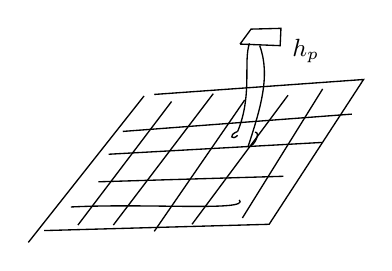
\begin{tikzpicture}[x=.010cm,y=-.010cm,font=\small,line width=.48pt]
\draw (6,303)--(153,117) (166,115)--(432,96)--(312,280)--(26,288);
\draw (69,281)--(188,124)
      (114,281)--(241,114)
      (166,289)--(281,122)
      (214,280)--(336,116)
      (278,272)--(380,108);
\draw (126,162)--(417,140)
      (108,191)--(379,176)
      (95,226)--(330,219)
      (60,258)..controls (160,253) and (289,264)..(274,249);
\draw (275,51)--(289,32)--(327,31)--(326,53)--(275,51);
\draw (287,50)..controls (279,73) and (291,116)..(272,162);
\draw (300,53)..controls (314,91) and (301,133)..(285,182);
\draw (272,162)..controls (259,167) and (265,174)..(272,167);
\draw (285,182)..controls (295,180) and (301,162)..(294,163);
\node[anchor=west] at (329,60) {$h_p$};
\end{tikzpicture}}\endgroup\par
У нижних концов вертикальных линий видны петли. Неясно, является ли одна из них буквой \(p\).}
\end{GelfandAdjacentEvidence}
\begin{GelfandAdjacentEvidence}{GELFAND-P001055}{4}

$p$ — квадратик

$h_p$ интерпрет. как высота пов. над плоскостью
\begin{equation*}
w(S)\equiv e^{-\beta\operatorname{ares}(S)},\quad\beta>0
\tag{2}
\end{equation*}
\SourceFigure{GELFAND-P001055}{area-operator-spelling}{В показателе написано \(\operatorname{ares}(S)\).}
\end{GelfandAdjacentEvidence}
\begin{GelfandAdjacentEvidence}{GELFAND-P001055}{5}

$\operatorname{ares} S$ — площадь того, что \dashuline{получ.}, если доп.
\dashuline{вертик.} стенками
\SourceFigure{GELFAND-P001055}{area-operator-word}{В пояснении также написано \(\operatorname{ares}\).}
\end{GelfandAdjacentEvidence}


(составить из твёрдых кубиков)
\begin{equation*}
=e^{-\beta|\Lambda|}\prod_{\langle p,p'\rangle}e^{-\beta|h_p-h_{p'}|},
\tag{3}
\end{equation*}
$h_p=0$ при $p\notin\Lambda$.

(гран. условие)


\Needspace{7\baselineskip}
\begin{GelfandAdjacentEvidence}{GELFAND-P001056}{1}
\SourcePage{GELFAND-P001056}{unlabelled}
\begin{equation*}
\mu(S)\equiv Z_\Lambda^{-1}w(S),\qquad Z_\Lambda=\sum_S' w(S).
\tag{4}
\end{equation*}
— распред. вероятностей.

Поведение типичных поверхностей — ?

\uwave{Результаты:} пусть \(E\) — мат. ожид. [вписано над строкой: по отн. к] распред. вер. \(\mu\) при \(\Lambda\nearrow Z^2\)
\Unclear{GELFAND-P001056}{expectation-correction}{Зачёркнутое слово после «мат. ожид.» читается неуверенно. Возможно «этого».}
\end{GelfandAdjacentEvidence}
\begin{GelfandAdjacentEvidence}{GELFAND-P001056}{2}


(а) \underline{для больших \(\beta\)} \(Eh_p^2\) ограничено
\begin{equation*}
\operatorname{Prob}\{h:|h_p|=n\}\sim e^{-\mathrm{const}\cdot n}
\tag{5}
\end{equation*}
(частн. случай общей теор. Добрушина)

(в) \(\beta\) \underline{мало}
\begin{equation*}
c_2\ln(|p-p'|+1)\leqslant E(h_p-h_{p'})^2\leqslant c_1\ln(|p-p'|+1)
\tag{6}
\end{equation*}
\SourceFigure{GELFAND-P001056}{fluctuation-bounds}{Левая граница имеет коэффициент \(c_2\), правая — \(c_1\).}
\end{GelfandAdjacentEvidence}
\begin{GelfandAdjacentEvidence}{GELFAND-P001056}{3}

\SourceFigure{GELFAND-P001056}{fluctuation-margin}{(сильно флуктуирует.) практически непрер. пов.}
\end{GelfandAdjacentEvidence}
\begin{GelfandAdjacentEvidence}{GELFAND-P001056}{4}


Enhancement of symm.

Уменьшаем квадратики \(\Rightarrow\) появл. непр. группа симметрий.
\Unclear{GELFAND-P001056}{symmetry-sentence}{Между «Уменьшаем» и «квадратики» зачёркнуты короткие знаки, возможно «кв».}
\end{GelfandAdjacentEvidence}
\begin{GelfandAdjacentEvidence}{GELFAND-P001056}{5}

(слишком сложно для объяснения)

\begin{equation*}
\mu(S)\sim\prod_{\langle p,p'\rangle}e^{-\beta|h_p-h_{p'}|}
\tag{7}
\end{equation*}
\(h_p\mapsto h_p+\mathrm{const}\)\qquad симметрия (непр.)

Наруш. гран. условиями.

Те же вопросы не сделаны при малых \(\beta\)

\begin{equation*}
Z_{\beta,\gamma}\equiv\sum_{S:\partial S=\gamma}w_\beta(S),\qquad
w_\beta(S)=e^{-\beta|S|}
\tag{8}
\end{equation*}
\begin{equation*}
\#\{S:\partial S=\gamma,\ |S|=\mathrm{area}\ S=n\}
  \sim C_\gamma^n n^{\delta(\gamma)},\quad n\text{ велико.}
\tag{9}
\end{equation*}
(из общих комбинаторных теорем)

Есть в статьях о методе Пайерлса.

\begin{equation*}
\ln C_\gamma\equiv\lim_{n\to\infty}\frac1n
 \ln\#\{S\mid\partial S=\gamma,\ |S|=n\}
\tag{10}
\end{equation*}
(11) \underline{Лемма} \(C_\gamma\) не зависит от \(\gamma\)

Гипотеза: зав. от топологич. св-в \(\gamma\):
\SourceFigure{GELFAND-P001056}{topology-sketches}{%
\begingroup\color{black}\GelfandFitDiagram{\begin{tikzpicture}[x=.013cm,y=-.013cm,line width=.55pt,font=\small]
\draw[rotate around={-30:(44,86)}] (44,86) ellipse [x radius=20,y radius=31];
\draw (26,101)--(57,66) (37,108)--(67,74) (48,107)--(72,85);
\node at (176,85) {или};
\draw[rotate around={22:(302,84)}] (302,84) ellipse [x radius=21,y radius=25];
\draw[rotate around={20:(403,81)}] (403,81) ellipse [x radius=17,y radius=23];
\draw (297,60)..controls (319,50) and (325,53)..(337,56)
    ..controls (358,64) and (383,67)..(401,59);
\draw (290,109)..controls (307,112) and (320,100)..(333,103)
    ..controls (357,111) and (377,116)..(396,104);
\draw (317,104)..controls (329,93) and (338,67)..(333,55)
 (327,105)--(348,61) (343,106)--(370,65)
 (355,108)--(382,65) (370,109)--(394,65);
\end{tikzpicture}}\endgroup}
\end{GelfandAdjacentEvidence}
\begin{GelfandAdjacentEvidence}{GELFAND-P001056}{6}


\(\delta(\gamma)\) определяет критич. явления; \(\delta(\gamma)\), видимо, зависит от топологии.
\Unclear{GELFAND-P001056}{delta-correction}{После первого \(\delta(\gamma)\) зачёркнута короткая запись, возможно «для».}
\end{GelfandAdjacentEvidence}
\begin{GelfandAdjacentEvidence}{GELFAND-P001056}{7}


\SourceFigure{GELFAND-P001056}{bottom-cancel}{\sout{Асимптотика (9).}}
\end{GelfandAdjacentEvidence}



\Needspace{7\baselineskip}
\begin{GelfandAdjacentEvidence}{GELFAND-P001057}{1}
\SourcePage{GELFAND-P001057}{27}
Трудный вопрос: как быть, если брать пов. с \(\forall\) топологией.

Сколько ручек имеет типичная поверхность?

\begin{equation*}
Z_{\beta,\gamma}<\infty\quad\text{при }\beta>\beta_0
\tag{12}
\end{equation*}
\Unclear{GELFAND-P001057}{inequality-12}{Знак отношения переписан. Возможно \(\beta>\beta_0\) или \(\beta\geqslant\beta_0\).}
\end{GelfandAdjacentEvidence}
\begin{GelfandAdjacentEvidence}{GELFAND-P001057}{2}


\begin{equation*}
Z_{\beta,\gamma}=+\infty\quad\text{при }\beta<\beta_0
  \qquad\text{(вроде газа)}
\tag{13}
\end{equation*}
\Unclear{GELFAND-P001057}{inequality-13}{Знак отношения переписан. Возможно \(\beta<\beta_0\) или \(\beta\leqslant\beta_0\).}
\end{GelfandAdjacentEvidence}
\begin{GelfandAdjacentEvidence}{GELFAND-P001057}{3}


(13): Плотность квадратов (в \(Z^3\)), принадл. пов., положительна

(как кривая Пеано)
\SourceFigure{GELFAND-P001057}{density-correction}{Сокращение «пов.» написано поверх штрихов.}
\end{GelfandAdjacentEvidence}
\begin{GelfandAdjacentEvidence}{GELFAND-P001057}{4}


Гипотеза, при \(\beta_0<\beta<\beta_R\) логарифм. флуктуации,

\(\beta>\beta_R\) — \uwave{roughening} (загрубление)

— фиксируется форма, почти гладкая (почти \(\mathrm{const}\))

Why bother?

\(1^\circ\) NaCl опис. этой моделью

\(2^\circ\) Эта теория эквив. калибр. теории \(SU(N)\) в пределе \uwave{\(N\Rightarrow0\)} (!) (вырожд. случай)
\SourceFigure{GELFAND-P001057}{gauge-limit}{После \(N\) видна двойная стрелка.}
\end{GelfandAdjacentEvidence}
\begin{GelfandAdjacentEvidence}{GELFAND-P001057}{5}


\(3^\circ\) It is a fun problem.
\Unclear{GELFAND-P001057}{fun-correction}{После «fun» зачёркнута короткая запись, возможно начало «pr».}
\end{GelfandAdjacentEvidence}
\begin{GelfandAdjacentEvidence}{GELFAND-P001057}{6}


\[
w_N(S)\underset{N\to0}{\longrightarrow}w(S)
\]
(москвичи любят разлагать по \(1/N\) при \(N\to\infty\)).

\uwave{Ссылки.}\quad \dashuline{Phys. Lett.}\quad
\uwave{Amos Maritan, C. Omero}

\underline{Обобщения}\(\rightarrow\)

Непр. случай: поверхн., не леж. на решётке.

Кусочно-лин. пов., сост. из \(\Delta\)-ков.

\begin{equation*}
w(S)=e^{-\beta\,\mathrm{area}(S)}
  \frac{\prod e^{-f\,\text{defect }\angle\,\text{at vertices}}}
       {e^{-c\,\#\,\text{handles of }S}}
  \prod_{\text{edges}}\frac{d\ell}{\ell}
\tag{14}
\end{equation*}
\Unclear{GELFAND-P001057}{weight-fraction}{Черта над нижней экспонентой передана как черта дроби. Её расположение видно в рукописи.}
\end{GelfandAdjacentEvidence}
\begin{GelfandAdjacentEvidence}{GELFAND-P001057}{7}


\SourceFigure{GELFAND-P001057}{regge-reference}{%
\begingroup\color{black}\GelfandFitDiagram{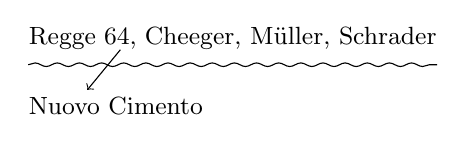
\begin{tikzpicture}[font=\small]
\node[anchor=west,inner sep=0pt] (regge) at (0,0) {Regge};
\node[anchor=west,inner sep=0pt] (year) at ([xshift=2.5pt]regge.east) {64,};
\node[anchor=west,inner sep=0pt] (names) at ([xshift=2.5pt]year.east) {Cheeger, Müller, Schrader};
\node[anchor=west,inner sep=0pt] (journal) at (0,-.85) {Nuovo Cimento};
\draw[->] (year.south)--(.75,-.65);
\draw[decorate,decoration={snake,amplitude=.65pt,segment length=8pt}]
    ([yshift=-.33cm]regge.west)--([yshift=-.33cm]names.east);
\end{tikzpicture}}\endgroup}
\end{GelfandAdjacentEvidence}


\uwave{Вопрос:} сходимость при сход. к непр. пов..

\[
R=\sum_f\text{area of }(d-2)\text{ simplex, }f\times\text{defect }\angle
\]
\begin{equation*}
\underline{\text{Theor.}}\quad R\longrightarrow\int\sqrt{g(x)}R(x)d^dx.
\tag{15}
\end{equation*}
\((14)\longrightarrow\) \uwave{теория струн Полякова}

\underline{Exercise:} Prove this!


\Needspace{7\baselineskip}
\begin{GelfandAdjacentEvidence}{GELFAND-P001058}{1}
\SourcePage{GELFAND-P001058}{unlabelled}
\uuline{1/\(\overline{\underline{\mathrm{XI}}}\)-82 г.}\qquad\underline{Сем. Гельфанда.}

\underline{Замолодчиков.}

Пусть
\[
[L_n,L_m]=(m-n)L_{n+m}+\frac{c}{12}\delta_{n+m,0}\mathbf1
  \qquad\text{(алгебра Вирасоро)}
\]
\Unclear{GELFAND-P001058}{virasoro-central}{В центральном члене видны только \(\frac{c}{12}\delta_{n+m,0}\mathbf1\).}
\end{GelfandAdjacentEvidence}
\begin{GelfandAdjacentEvidence}{GELFAND-P001058}{2}

и сущ. такой вектор \(\lvert0\rangle\), что
\begin{gather*}
L_n\lvert0\rangle=0,\quad n>0,\\
L_0\lvert0\rangle=\Delta\lvert0\rangle.
\end{gather*}
причём
\[
\prod_i(L_{-n_i})^{s_i}\lvert0\rangle=\lvert\psi\rangle
\]
\Unclear{GELFAND-P001058}{vector-correction}{После \(L\) зачёркнут индекс, возможно \(n_i\) или \(m_i\). Ниже вписано \(-n_i\).}
\end{GelfandAdjacentEvidence}
\begin{GelfandAdjacentEvidence}{GELFAND-P001058}{3}

(все векторы так получаются)

Пусть \(\varphi(z)\) — оператор, действ. в этом пр-ве и
\[
[L_n,\varphi(z)]=z^{n+1}\frac{d\varphi(z)}{dz}+(n+1)\Delta z^n\varphi(z)
\]
Он опрд. этой ф-лой однозначно.

\dashuline{1-й вопрос}: что можно о нём сказать?

— как посчитать
\[
\langle0\lvert\varphi(z_1)\ldots\varphi(z_n)\rvert0\rangle\quad ?
\]
\(L_{-n}^{+}=L_n\), \(\langle0\mid0\rangle=1\Rightarrow\) восстан. скал. произведение.

\dashuline{2-й вопрос}: какие есть соотношения на состояния, к-рые можно написать?

Или: неприводим ли этот модуль?

\underline{Ответ:} (Неретин) вырожд., если \(\exists\) натур. \(\alpha,\beta\), что
\Unclear{GELFAND-P001058}{answer-correction}{Перед «вырожд.» зачёркнуто, по-видимому, «неприв., если».}
\end{GelfandAdjacentEvidence}
\begin{GelfandAdjacentEvidence}{GELFAND-P001058}{4}

\begin{gather*}
\left(-\Delta+\frac{\beta^2-1}{24}(c-13)+\frac{(\alpha\beta-1)}{2}\right)
\left(-\Delta+\frac{(\alpha^2-1)}{24}(c-13)+\frac{(\alpha\beta-1)}{2}\right)\\
{}+\frac{(\alpha^2-\beta^2)^2}{16}=0.
\end{gather*}
\SourceFigure{GELFAND-P001058}{kac-formula-left}{Первый множитель содержит \(\beta^2-1\).}
\end{GelfandAdjacentEvidence}
\begin{GelfandAdjacentEvidence}{GELFAND-P001058}{5}

\SourceFigure{GELFAND-P001058}{kac-formula-right}{Второй множитель содержит \(\alpha^2-1\).}
\end{GelfandAdjacentEvidence}
\begin{GelfandAdjacentEvidence}{GELFAND-P001058}{6}

Вырожд. наступает на \underline{уровне \(\alpha\beta\)}.

\(\vec{x}(\xi_1,\xi_2)\) — поверхность, \(g_{ab}(\xi_1,\xi_2)\) — метрика, \(a,b=1,2\).
\SourceFigure{GELFAND-P001058}{metric-margin}{\(\mathord{//}\) \(x,g\) счит. независ. перем. (метрика — не индуцир.)}
\end{GelfandAdjacentEvidence}
\begin{GelfandAdjacentEvidence}{GELFAND-P001058}{7}


Пусть
\begin{multline*}
Z\equiv\int\mathcal{D}\vec{x}\,\mathcal{D}g_{ab}\,
\exp\left\{-\tfrac12\int\sqrt{g}\,g^{ab}\partial_a\vec{x}\,\partial_b\vec{x}\,d^2\xi\right\}\\
\exp\left\{-\mu_0^2\int\sqrt{g}\,d^2\xi\right\}.
\tag{1}
\end{multline*}
Вычисление — ?

Инв. отн. преобр.
\[
\begin{cases}
\xi^a\mapsto\xi^a+\varepsilon^a(\xi),\\
g_{ab}(\xi)\mapsto g_{ab}+\nabla_a\varepsilon_b+\nabla_b\varepsilon_a.
\end{cases}
\]
Делим на эту группу (элем. объёма подразумев. факторизованным)

— надо интегр. по орбитам.

\SourceFigure{GELFAND-P001058}{orbit-sketch}{%
\begingroup\color{black}\GelfandFitDiagram{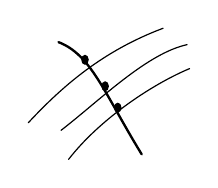
\begin{tikzpicture}[x=.016cm,y=-.016cm,line cap=round]
\draw[line width=.43pt]
  (9,118)..controls(36,89)and(68,61)..(116,43)
  (35,124)..controls(66,100)and(103,63)..(135,56)
  (41,147)..controls(65,116)and(106,88)..(137,75);
\draw[line width=.85pt]
  (33,54)..controls(59,64)and(69,94)..(99,143);
\fill (54,68) ellipse [x radius=3,y radius=4];
\fill (70,89) ellipse [x radius=3,y radius=4];
\fill (80,106) ellipse [x radius=3,y radius=4];
\end{tikzpicture}}\endgroup\par
На трёх пересечениях видны утолщения. Наличие наконечников стрелок неясно.}
\end{GelfandAdjacentEvidence}
\begin{GelfandAdjacentEvidence}{GELFAND-P001058}{8}

Представитель: \(\vec{x}(\xi)\) — любое,\quad \(g_{ab}(\xi)=\delta_{ab}\rho(\xi)\)

Получается:
\begin{equation*}
Z=\mathrm{const}\int\mathcal{D}\varphi\,[\det(\Delta_g)]^{-D/2}\,[\det\mathcal{L}]^{1/2},
\tag{2}
\end{equation*}
\Unclear{GELFAND-P001058}{integral-measure}{У знака после \(\mathcal D\) видна петля справа. Здесь он передан как \(\varphi\), возможно \(\psi\).}
\end{GelfandAdjacentEvidence}



\Needspace{7\baselineskip}
\begin{GelfandAdjacentEvidence}{GELFAND-P001059}{1}
\SourcePage{GELFAND-P001059}{38}
где
\Unclear{GELFAND-P001059}{top-cancelled-label}{В верхнем поле зачёркнута короткая запись. Точное чтение не установлено.}
\end{GelfandAdjacentEvidence}
\begin{GelfandAdjacentEvidence}{GELFAND-P001059}{2}


\begin{equation*}
(\mathcal L\varepsilon)_a
=\nabla^b\bigl(\nabla_a^a\varepsilon_b+\nabla_b\varepsilon_a
   -g_{ab}\nabla^c\varepsilon_c\bigr).
\tag{3}
\end{equation*}
\Unclear{GELFAND-P001059}{first-derivative}{У первой \(\nabla\) в скобках видны нижний \(a\) и утолщённый верхний знак, похожий на \(a\). Возможно, верхний знак зачёркнут.}
\end{GelfandAdjacentEvidence}
\begin{GelfandAdjacentEvidence}{GELFAND-P001059}{3}

\Unclear{GELFAND-P001059}{first-term-cancellation}{После первого \(\varepsilon_b\) зачёркнута вертикальная запись.}
\end{GelfandAdjacentEvidence}
\begin{GelfandAdjacentEvidence}{GELFAND-P001059}{4}


В итоге, вычисляя, получаем:

\SourceFigure{GELFAND-P001059}{field-notation}{Одинаковый знак с петлёй справа стоит в формулах (4), (6) и \(\rho=e^\varphi\). Он передан через \(\varphi\), возможно \(\psi\).}
\end{GelfandAdjacentEvidence}
\begin{GelfandAdjacentEvidence}{GELFAND-P001059}{5}


\(D\) — размерность пр-ва, \(D<26\).
\begin{equation*}
Z=\int\mathcal D\varphi\cdot
  \exp\left\{-\frac{26-D}{48\pi}\int
  \left[\frac12\partial_a\varphi\,\partial_a\varphi+
  m_0^2e^\varphi\right]d^2\xi\right\}.
\tag{4}
\end{equation*}
\(\varphi\) из ф-лы: \(\rho=e^{\varphi}\).
\[
\Delta_g=\frac{1}{\sqrt g}\partial_a
  \bigl(\sqrt g\,g^{ab}\partial_b\bigr).
\]

Задача о струне будет решена, если вычислить этот интеграл.

\(D=26\Rightarrow\) ответ такой же, как при \(g_{ab}=\delta_{ab}\).

Это предпис. использ. в дуальных моделях. Они точны при \(D=26\).

По каким пов. надо интегрировать?

Натян. пов. на 2 контура (эволюц. контура).
\Unclear{GELFAND-P001059}{surface-abbreviation}{Начало строки перед «пов.» читается как сокращение «Натян.».}
\end{GelfandAdjacentEvidence}
\begin{GelfandAdjacentEvidence}{GELFAND-P001059}{6}

\SourceFigure{GELFAND-P001059}{cylinder-contours}{%
\begingroup\color{black}\GelfandFitDiagram{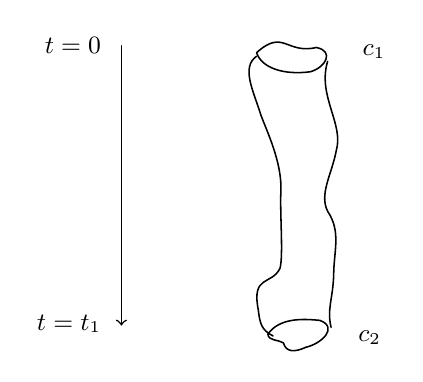
\begin{tikzpicture}[x=.011cm,y=-.011cm,font=\small,line width=.56pt,line cap=round]
\draw[->] (116,40)--(116,363);
\node[anchor=east] at (104,40) {$t=0$};
\node[anchor=east] at (104,361) {$t=t_1$};
\draw (272,48)..controls(303,20)and(306,50)..(341,42)
  ..controls(362,46)and(352,65)..(334,70)
  ..controls(304,74)and(278,66)..(272,48);
\draw (272,52)..controls(254,65)and(268,91)..(277,120)
  ..controls(284,139)and(302,176)..(300,209)
  ..controls(299,237)and(303,282)..(299,297)
  ..controls(289,317)and(266,304)..(274,345)
  ..controls(276,362)and(278,368)..(291,375);
\draw (354,58)..controls(342,98)and(373,130)..(364,161)
  ..controls(359,188)and(344,211)..(354,231)
  ..controls(370,255)and(361,277)..(361,305)
  ..controls(360,333)and(353,344)..(358,365);
\draw (285,373)..controls(298,354)and(325,355)..(345,357)
  ..controls(367,365)and(347,384)..(329,388)
  ..controls(316,394)and(306,394)..(303,383)
  ..controls(297,379)and(286,381)..(285,373);
\node[anchor=west] at (383,47) {$c_1$};
\node[anchor=west] at (378,377) {$c_2$};
\end{tikzpicture}}\endgroup}
\end{GelfandAdjacentEvidence}
\begin{GelfandAdjacentEvidence}{GELFAND-P001059}{7}

\begin{equation*}
Z(c_1,c_2,t_1)\underset{t_1\to\infty}{=}
  \sum_nG(c_1,n)\,G(c_2,n)\,e^{-E_nt_1}.
\tag{5}
\end{equation*}

Спектр стац. состояний в теории Лиувилля — спектр КТП для лагранжиана
\Unclear{GELFAND-P001059}{liouville-cancellation}{Над словами «теории Лиувилля» зачёркнута запись.}
\end{GelfandAdjacentEvidence}
\begin{GelfandAdjacentEvidence}{GELFAND-P001059}{8}

\begin{equation*}
\int_M\left[\frac12\partial_a\varphi\,\partial_a\varphi+
  m_0^2e^\varphi\right]d^2\xi.
\tag{6}
\end{equation*}

\uwave{Гипотеза:} спектр связан с системой \(L_n\), опис. на предыд. странице.
\begin{gather*}
z=\xi_1+i\xi_2,\\
\bar z=\xi_1-i\xi_2.
\end{gather*}
Бесследный 2-мерный сохр. тензор эн.-импульса:
\[
T_{ab}=\partial_a\varphi\,\partial_b\varphi
   -\tfrac12\delta_{ab}(\partial_c\varphi)^2
   +\alpha\partial_a\partial_b\varphi-\beta\delta_{ab}(\partial_c\varphi)^2.
\]
\SourceFigure{GELFAND-P001059}{tensor-last-term}{Последнее слагаемое читается \(-\beta\delta_{ab}(\partial_c\varphi)^2\).}
\end{GelfandAdjacentEvidence}
\begin{GelfandAdjacentEvidence}{GELFAND-P001059}{9}

\begin{align*}
T&=\varphi_z^2+2\varphi_{zz},&
\partial_{\bar z}T&=0,\\
\bar T&=\varphi_{\bar z}^2+2\varphi_{\bar z\bar z},&
\partial_zT&=0.
\end{align*}
\Unclear{GELFAND-P001059}{tensor-cancelled-index}{У первого \(T\) зачёркнут нижний индекс, возможно \(zz\).}
\end{GelfandAdjacentEvidence}
\begin{GelfandAdjacentEvidence}{GELFAND-P001059}{10}

\SourceFigure{GELFAND-P001059}{lower-holomorphic}{Во втором равенстве справа над \(T\) нет дополнительной черты.}
\end{GelfandAdjacentEvidence}
\begin{GelfandAdjacentEvidence}{GELFAND-P001059}{11}


\[
\underbrace{T(z)=\sum_{n=-\infty}^{\infty}z^{n-2}L_n}_{\text{(разлаг. в ряд)}}
\qquad\text{— отсюда берутся }L_n!
\]
\SourceFigure{GELFAND-P001059}{series-bracket}{Ряд и его левая часть заключены в нижнюю скобку.}
\end{GelfandAdjacentEvidence}



\Needspace{7\baselineskip}
\begin{GelfandAdjacentEvidence}{GELFAND-P001060}{1}
\SourcePage{GELFAND-P001060}{unlabelled}
\uuline{Бейлинсон А.}

\underline{И.М.Г.} Гельфанд, Пономарёв (УМН, \(\underset{\text{\scriptsize[2?]}}{\sim}1968\) г.)
свед. опис. неразлож. предст. гр. Лоренца к задаче лин. алгебры.
\Unclear{GELFAND-P001060}{reference-leading-mark}{Перед «УМН» зачёркнута короткая помета.}
\end{GelfandAdjacentEvidence}
\begin{GelfandAdjacentEvidence}{GELFAND-P001060}{2}

\Unclear{GELFAND-P001060}{reference-lower-mark}{Под знаком \(\sim\) виден знак, похожий на \(2\).}
\end{GelfandAdjacentEvidence}
\begin{GelfandAdjacentEvidence}{GELFAND-P001060}{3}


\underline{Б.}\quad\uwave{модельный пример.} — \(\mathrm{SL}(2,\mathbb R)\)

На \(\mathbb P^1\) надо классиф. \(D\)-модули с особ. в фикс. \(2^{\text{х}}\) точках.

\underline{Теорема 1.} катег. \(D\)-модулей в диске с фикс. особ. эквивалентна катег.
\SourceFigure{GELFAND-P001060}{pointed-disk}{%
\begingroup\color{black}\GelfandFitDiagram{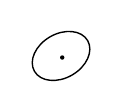
\begin{tikzpicture}[x=1cm,y=1cm,line width=.5pt]
\draw[rotate=30] (0,0) ellipse [x radius=.39,y radius=.28];
\fill (.015,-.02) circle [radius=.028];
\end{tikzpicture}}\endgroup}
\end{GelfandAdjacentEvidence}
\begin{GelfandAdjacentEvidence}{GELFAND-P001060}{4}

\SourceFigure{GELFAND-P001060}{disk-and-pair}{%
\begingroup\color{black}\GelfandFitDiagram{\begin{tikzpicture}[font=\small,line width=.48pt]
\node (linear) at (.65,.64) {лин. отобр.};
\node[anchor=west] at (linear.north west) {\scriptsize пар};
\node (psi) at (.2,-.22) {$\Psi$};
\node (phi) at (2.07,-.22) {$\Phi$};
\draw[->] (.58,-.15)--node[above]{$u$}(1.72,-.15);
\draw[->] (1.72,-.32)--node[below]{$v$}(.58,-.32);
\draw (linear.west)..controls(-.23,.37)and(.3,.28)..(1.28,.29)
  ..controls(1.5,.31)and(1.36,.12)..(1.38,.01);
\end{tikzpicture}}\endgroup\par
Над «лин. отобр.» вписано «пар».}
\end{GelfandAdjacentEvidence}
\begin{GelfandAdjacentEvidence}{GELFAND-P001060}{5}

таких что \(uv-\mathrm{Id}\) \uwave{обратимо}.
\SourceFigure{GELFAND-P001060}{bracketed-description}{%
\(\left[\left(\begin{array}{l}
 \text{вне }0\text{ — гладкие }=\\
 =\text{рассл. со связностью};\\
 \text{в }0\text{ — регулярная особ..}
\end{array}\right)\right]\)}
\end{GelfandAdjacentEvidence}
\begin{GelfandAdjacentEvidence}{GELFAND-P001060}{6}


\underline{Геом. задача.}
\SourceFigure{GELFAND-P001060}{geometric-inclusions}{%
\begingroup\color{black}\GelfandFitDiagram{\begin{tikzcd}[ampersand replacement=\&,column sep=small]
Y \arrow[r,hook,"i"] \& X \& U=X\setminus Y \arrow[l,hook',"j"']
\end{tikzcd}}\endgroup}
\end{GelfandAdjacentEvidence}
\begin{GelfandAdjacentEvidence}{GELFAND-P001060}{7}

Пучок на \(X\) зад. так:
\[
\mathcal F_X=(\mathcal F_U,\mathcal F_Y,\quad
  \mathcal F_Y\longrightarrow i^*j_*\mathcal F_U)
\]
(ф-я склейки)
\Unclear{GELFAND-P001060}{gluing-cancellation}{Между «ф-я» и «склейки» зачёркнута короткая запись, возможно начало «ск».}
\end{GelfandAdjacentEvidence}
\begin{GelfandAdjacentEvidence}{GELFAND-P001060}{8}


Для представл. надо решить аналог. задачу на пр-ве флагов.

\Unclear{GELFAND-P001060}{cancelled-equation}{Зачёркнутая формула, возможно \(Y=f^{-1}(0)\).}
\end{GelfandAdjacentEvidence}
\begin{GelfandAdjacentEvidence}{GELFAND-P001060}{9}


\underline{Теор.} катег. \(D\)-модулей с регул. особ. на \(X\) эквивал. катег. наборов
\SourceFigure{GELFAND-P001060}{module-pair}{%
\begingroup\color{black}\GelfandFitDiagram{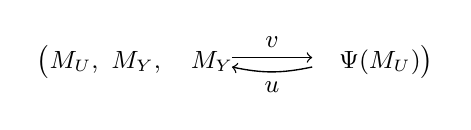
\begin{tikzpicture}[font=\small,line width=.49pt]
\node at (0,0) {$\bigl(M_U,\ M_Y,\quad M_Y$};
\node at (3.19,0) {$\Psi(M_U)\bigr)$};
\draw[->] (1.23,.055)--node[above]{$v$}(2.25,.055);
\draw[->] (2.25,-.065) to[bend left=12] node[below]{$u$}(1.23,-.065);
\end{tikzpicture}}\endgroup}
\end{GelfandAdjacentEvidence}
\begin{GelfandAdjacentEvidence}{GELFAND-P001060}{10}

\(vu=N\) — что-то.
\Unclear{GELFAND-P001060}{bottom-cancellation}{После «что-то» зачёркнута короткая запись.}
\end{GelfandAdjacentEvidence}



\Needspace{7\baselineskip}
\begin{GelfandAdjacentEvidence}{GELFAND-P001061}{1}
\SourcePage{GELFAND-P001061}{48}
\uuline{15/\(\overline{\underline{\mathrm{XI}}}\)-82 г.}\qquad\underline{Сем. Гельфанда.}

\uuline{И.М.Г.}\quad\underline{Задача}. (неточная)

\(G_{n,k}\) — грассм. мн-ие, \(k\)-мерн. плоск. в \(n\)-мерн. пр-ве.
\Unclear{GELFAND-P001061}{top-cancelled-symbol}{В начале строки зачёркнута запись, похожая на \(G\) с дополнительными знаками.}
\end{GelfandAdjacentEvidence}
\begin{GelfandAdjacentEvidence}{GELFAND-P001061}{2}


Когом. счит. с пом. клеток Шуберта.
\Unclear{GELFAND-P001061}{schubert-initial-phrase}{Начало строки читается предположительно как «Когом. счит.».}
\end{GelfandAdjacentEvidence}
\begin{GelfandAdjacentEvidence}{GELFAND-P001061}{3}


({} \dashuline{Клетка} зад. размерностями пересеч. с флагом
\begin{gather*}
0=d_0\leqslant d_1\leqslant d_2\leqslant\ldots\leqslant d_n=k,\\
\dim\text{ клетки}=\sum d_j.
\end{gather*}
)
\SourceFigure{GELFAND-P001061}{schubert-dimension}{В формуле размерности записано \(\sum d_j\).}
\end{GelfandAdjacentEvidence}
\begin{GelfandAdjacentEvidence}{GELFAND-P001061}{4}


Рассм. \(\mathrm{II}_1\)-фактор; в нём рассм. \(\alpha\)-мерные проекторы (конт. аналог грассм. мн-ий).
\uwave{Есть ли аналог клетки Шуберта?}

\uwave{Флаг непр. размерности \([0,1]\).}

Получ. грассм. мн-ие?

Непр. когомологии!?

\uwave{Гипотеза}: описыв. монот. ф-ями.
\Unclear{GELFAND-P001061}{hypothesis-cancellation}{После «Гипотеза» зачёркнута короткая запись.}
\end{GelfandAdjacentEvidence}
\begin{GelfandAdjacentEvidence}{GELFAND-P001061}{5}


Ещё более расплывчатый вопрос: какая топология? и какие когомологии?
\Unclear{GELFAND-P001061}{question-leading-cancellation}{Перед «Ещё» зачёркнут знак.}
\end{GelfandAdjacentEvidence}
\begin{GelfandAdjacentEvidence}{GELFAND-P001061}{6}


\uuline{Ю.И. Манин.}

1) Флаговые супермногообразия

2) Преобр. Радона–Пенроуза в суперматем. ситуации.
\Unclear{GELFAND-P001061}{agenda-cancelled-letter}{Между «в» и «суперматем.» зачёркнут одиночный знак.}
\end{GelfandAdjacentEvidence}
\begin{GelfandAdjacentEvidence}{GELFAND-P001061}{7}


3) Прилож. к решению нелин. ур-й: новые реш. неавтодуальных ур-й ЯМ

(обычные и суперсимм.)

4) Конкретные флаговые мн-ия, их искривление и т.п. в суперсимметрии и супергравитации.

5) Задача об индексе и о характеристич. классах.
\SourceFigure{GELFAND-P001061}{agenda-annotations}{[Под «об индексе»:] (не сделана по настоящему)\par [Под «о характеристич. классах»:] (что-то важное сделал А.С. Шварц)}
\end{GelfandAdjacentEvidence}
\begin{GelfandAdjacentEvidence}{GELFAND-P001061}{8}


Будет об 1)–4)

\medskip
1) \underline{Напоминание об автодуальных ур-ях Я.М.}

\(T=\mathbb C^4\)\qquad [антиголом. инвол. \(T\oplus T^*\)]
\SourceFigure{GELFAND-P001061}{involution-abbreviation}{Первое сокращение читается как «антиголом.».}
\end{GelfandAdjacentEvidence}
\begin{GelfandAdjacentEvidence}{GELFAND-P001061}{9}

\SourceFigure{GELFAND-P001061}{involution-relation}{Между \(T\) и \(T^*\) написано \(\oplus\).}
\end{GelfandAdjacentEvidence}
\begin{GelfandAdjacentEvidence}{GELFAND-P001061}{10}


\(\dim G(2,T)=4\) = комплексное компактное пр-во Минковского.

3-мерн. клетка (сем-во, параметр., [разн.?] группой)
\Unclear{GELFAND-P001061}{three-cell-description}{Сокращение перед «группой» может читаться «разн.» или «разл.».}
\end{GelfandAdjacentEvidence}
\begin{GelfandAdjacentEvidence}{GELFAND-P001061}{11}


\SourceFigure{GELFAND-P001061}{cone-sketch}{%
\begingroup\color{black}\GelfandFitDiagram{\begin{tikzpicture}[x=.010cm,y=-.010cm,font=\small,line width=.55pt]
\node[anchor=east] at (-104,-8) {$C^3(x)$};
\draw (-69,-27)--(0,0)--(-82,28);
\draw[rotate around={27:(-78,0)}] (-78,0) ellipse [x radius=13,y radius=29];
\draw (0,0)--(70,-28) (0,0)--(73,23);
\draw (76,-1) ellipse [x radius=12,y radius=26];
\draw (87,23)--(98,23);
\fill (0,0) circle [radius=3.2];
\node[below] at (0,3) {$x$};
\draw[->] (-99,79)..controls(-64,74)and(-38,61)..(-16,34);
\node[anchor=east] at (-105,80) {Вершина конуса:};
\end{tikzpicture}}\endgroup\par
(опред. точкой).}
\end{GelfandAdjacentEvidence}
\begin{GelfandAdjacentEvidence}{GELFAND-P001061}{12}


\[
M^4=\text{вещ. часть }G(2,T)\setminus C^3(\infty)
\ \leftarrow\ \infty\text{-конус}.
\]

2-мерн. клетки: 2 сорта

\[
C^2_{\underset{+}{\alpha},\underset{-}{\beta}}
  (x,\mathbb C^2\subset T_xM)
  \text{ — }\pm\text{-плоскости},\quad(\alpha,\beta)\text{-плоскости}.
\]
\SourceFigure{GELFAND-P001061}{plane-symbol}{Внутри скобок перед \(\subset\) видна \(\mathbb C\) с верхним индексом \(2\).}
\end{GelfandAdjacentEvidence}
\begin{GelfandAdjacentEvidence}{GELFAND-P001061}{13}

\SourceFigure{GELFAND-P001061}{plane-signs}{Знак \(+\) написан под \(\alpha\), знак \(-\) под \(\beta\).}
\end{GelfandAdjacentEvidence}



\Needspace{7\baselineskip}
\begin{GelfandAdjacentEvidence}{GELFAND-P001062}{1}
\SourcePage{GELFAND-P001062}{unlabelled}
\(C^1\) — нулевые прямые (лучи света)

\SourceFigure{GELFAND-P001062}{tautological-bundles}{%
\begingroup\color{black}\GelfandFitDiagram{\begin{tikzpicture}[font=\small,line width=.5pt]
\node (base) at (1.4,-.8) {$G(2,T)$};
\node (left) at (.86,.97) {$\zeta$};
\node (right) at (3.09,.9) {$\tilde{\zeta}\subset T^*$};
\node (dual) at (3.01,-.32) {$\zeta^*$};
\draw[->] (left.south)--(1.24,-.39);
\draw[->] (2.52,.66)--(1.92,-.37);
\draw (2.68,.34)--(2.72,.17) (2.78,.37)--(2.82,.13);
\node[align=center,text width=2.6cm] at (-.49,-.95) {тавтол. рассл.\\(2-компон. спиноры)};
\draw[->] (-.45,-.32)--(.41,.42);
\end{tikzpicture}}\endgroup\par
Знак расслоения условно передан через \(\zeta\). Значение двух черт под правой подписью не установлено.}
\end{GelfandAdjacentEvidence}
\begin{GelfandAdjacentEvidence}{GELFAND-P001062}{2}


\underline{Задача.}\qquad \(G(2,T)\)

Описать супероднородные компл. мн-зия \(M\), для к-рых \(M_{\mathrm{red}}=G(2,T)\).

Усл.: \(M\) — флаговое мн-зие для простых супергрупп Ли классического типа.

\underline{Список (начало)}.

\[
\text{а)}\quad F(2|0,2|N,\mathbb C^{4|N})=M
\]
\Unclear{GELFAND-P001062}{cancelled-flag-argument}{После \(2\mid N\) зачёркнут знак, похожий на \(2\).}
\end{GelfandAdjacentEvidence}
\begin{GelfandAdjacentEvidence}{GELFAND-P001062}{3}

(флаги разм. \(2|0,2|N\) в \(\mathbb C^{4|N}\)).
\[
N=0,1,2,3,\ldots
\qquad
\mathbb C^{4|N}=(\mathbb C^4)_0\oplus(\mathbb C^N)_1.
\]
\SourceFigure{GELFAND-P001062}{superdimension-arrow}{%
\begingroup\color{black}\GelfandFitDiagram{\begin{tikzpicture}[font=\small,line width=.48pt]
\draw[->] (1.48,.3)..controls(1.15,1.3)and(.78,1.22)..(-.25,1.36);
\draw (0,.24)--(-.05,-.4) (.1,.24)--(.05,-.4);
\node[align=left,anchor=west] at (.2,-.05) {размерность\\$=4|4N$};
\end{tikzpicture}}\endgroup\par
Справа от цепочки включений написано «размерность \(=4\mid4N\)»; стрелка направлена вверх и влево.}
\end{GelfandAdjacentEvidence}
\begin{GelfandAdjacentEvidence}{GELFAND-P001062}{4}


Наивное опред.:
\[
\text{точки }x\in F(2|0,2|N,\mathbb C^{4|N})
  =\underline{\mathbb C^{2|0}\subset\mathbb C^{2|N}}\subset\mathbb C^{4|N}.
\]
Но: нехватает координат.

\uwave{Правильное опред.}: \(\forall\) суперкоммут. \(\mathbb C\)-алгебры \(A\) задаётся \(M(A)\)
и теперь ещё задаются \([A\overset f\longrightarrow B]\)
\[
\begin{array}{r@{\quad}l}
M(A):={}&N^{2|0}\subset N^{2|N}\subset A\otimes_{\mathbb C}\mathbb C^{4|N}\\
\downarrow&\text{(проективные)}\\
M(B)&\text{прямые подмодули}
\end{array}
\]
\SourceFigure{GELFAND-P001062}{functor-diagram}{Стрелка направлена от \(M(A)\) к \(M(B)\), а подпись о подмодулях помещена под цепочкой включений.}
\end{GelfandAdjacentEvidence}
\begin{GelfandAdjacentEvidence}{GELFAND-P001062}{5}


\dashuline{Координаты:}\quad
\(G(1|0,\mathbb C^{m|n}):=P^{m-1|n}\supset P\).
\SourceFigure{GELFAND-P001062}{projective-point-symbol}{Справа после \(\supset\) знак, по-видимому, \(P\).}
\end{GelfandAdjacentEvidence}
\begin{GelfandAdjacentEvidence}{GELFAND-P001062}{6}


Однородные коорд-ты: \((x_1,\ldots,x_m;\xi_1,\ldots,\xi_n)\).
\[
\text{Покрытие } P^{m-1,n}=\bigcup_{i=1}^{m}U_i,\quad
U_i:\left(\frac{x_1}{x_i},\ldots,\frac{x_m}{x_i},
          \frac{\xi_1}{x_i},\ldots,\frac{\xi_m}{x_i}\right).
\]
\SourceFigure{GELFAND-P001062}{affine-first-odd}{В знаменателе первой нечётной координаты, по-видимому, \(x_i\).}
\end{GelfandAdjacentEvidence}
\begin{GelfandAdjacentEvidence}{GELFAND-P001062}{7}

\SourceFigure{GELFAND-P001062}{affine-last-index}{В последней дроби написано \(\xi_m/x_i\), при \(\xi_n\) в списке однородных координат.}
\end{GelfandAdjacentEvidence}
\begin{GelfandAdjacentEvidence}{GELFAND-P001062}{8}


\uwave{Упражнение}: связать с предыдущим (большие клетки).

\uwave{Бывают:} \(\xi_i=0\) — клетка коразмерности \(0|1\).

Неизвестно, в каких когомологиях они лежат?

Дифф. и интегр. форм тоже не хватает. (они обслуж. крайние разм.)
\Unclear{GELFAND-P001062}{forms-abbreviation}{Сокращение читается предположительно как «обслуж.».}
\end{GelfandAdjacentEvidence}
\begin{GelfandAdjacentEvidence}{GELFAND-P001062}{9}


Шварцевские объекты промеж., но облад. странными св-вами.

Вещественные точки большой клетки в \(F(2|0,2|N;\mathbb C^{4|N})=\)
\[
=N\text{-расширенное }\underline{\text{суперпр-во физиков}}:
 (x^m;\theta_{\alpha i},\theta^{\beta i}).
\]
\dashuline{Требование}: [вписано сущ.] \sout{конформное}
конформного пополнения.
\SourceFigure{GELFAND-P001062}{completion-insertion}{«сущ.» вписано со знаком вставки. Прежнее «конформное» зачёркнуто.}
\end{GelfandAdjacentEvidence}
\begin{GelfandAdjacentEvidence}{GELFAND-P001062}{10}


\[
\text{б)}\quad FI(2|0,2|2,\mathbb C^{4|4},\Pi\mathrm{Sp})
  \qquad \text{размерность}=4|8.
\]
\Unclear{GELFAND-P001062}{cancelled-isotropic-argument}{Перед \(\mathbb C^{4\mid4}\) зачёркнута запись, возможно \(\mathrm{OSp}\).}
\end{GelfandAdjacentEvidence}



\Needspace{7\baselineskip}
\begin{GelfandAdjacentEvidence}{GELFAND-P001063}{1}
\SourcePage{GELFAND-P001063}{49}
\(I\) — изотропные,\quad \(\Pi\mathrm{Sp}\) — тип формы, отн. к-рой флаги изотропны.

(нечетная симм. форма)

Еще есть \underline{серии} и \underline{изолир.} мн-зия.
\Unclear{GELFAND-P001063}{cancelled-word}{Перед «Еще» зачёркнуто слово, возможно «Бывают» или «Будут».}
\end{GelfandAdjacentEvidence}


\[
2)\quad M=G(2,T),\qquad \underline{P(T)}=\underline{G(1,T)}.
\]


\Needspace{7\baselineskip}
\begin{GelfandAdjacentEvidence}{GELFAND-P001064}{1}
\SourcePage{GELFAND-P001064}{unlabelled}
\underline{22/\(\overline{\underline{\mathrm{XI}}}\)-82 г.}\qquad
\uuline{Сем. Гельфанда.}

\uuline{А. М. Поляков.}

(Ал-др Маркович).

Зад. о струне
\SourceFigure{GELFAND-P001064}{string-caption}{%
\begingroup\color{black}\GelfandFitDiagram{\begin{tikzpicture}[x=.031cm,y=-.031cm,line width=.55pt]
\draw (51,13)..controls(75,18)and(102,23)..(115,41)
 ..controls(139,80)and(104,108)..(81,111)
 ..controls(47,110)and(30,95)..(30,77)
 ..controls(28,63)and(7,21)..(41,13);
\end{tikzpicture}}\endgroup\par
— элем. возбужд..}
\end{GelfandAdjacentEvidence}
\begin{GelfandAdjacentEvidence}{GELFAND-P001064}{2}


Сводится к следующему: есть поле
\[
\varphi=\varphi(\xi_1,\xi_2)\qquad
  (\sim\text{ пов. в изотермич. коорд.})
\]
\begin{equation*}
g_{ab}(\xi)=e^{\varphi(\xi)}\delta_{ab}.
\tag{1}
\end{equation*}
\begin{equation*}
\mathcal L=\frac1\gamma\left\{\frac12(\partial_a\varphi)^2+e^\varphi\right\},
\qquad S=\int\mathcal L\,d^2\xi,
\tag{2}
\end{equation*}
\begin{equation*}
\frac1\gamma=\frac{26-D}{48\pi}
\tag{3}
\end{equation*}
(\(D\) — разм. пр-ва, в к-рое вклад. рассм. 2-мерная пов.)

Откуда вид (2) (кроме \(\gamma\))?

Фиксир. метрику (1). Остаётся свобода: конформные преобр..
\begin{equation*}
e^{\widetilde\varphi(z,\bar z)}
=\left|\frac{dw}{dz}\right|^2 e^{\varphi(w(z),\overline w(z))}.
\tag{4}
\end{equation*}
\SourceFigure{GELFAND-P001064}{conformal-last-argument}{В правом показателе черта стоит над вторым \(w\), а последний \(z\) без черты.}
\end{GelfandAdjacentEvidence}
\begin{GelfandAdjacentEvidence}{GELFAND-P001064}{3}

\SourceFigure{GELFAND-P001064}{transformation-margin}{Справа от формулы видно «(2)» с дополнительным штрихом.}
\end{GelfandAdjacentEvidence}
\begin{GelfandAdjacentEvidence}{GELFAND-P001064}{4}


Лагр. (2) — единств. лок. лагранжиан (завис. лишь от знач. ф-и и её произв. в точке), не меняющийся при преобр. (4).

\(\mathcal L\) наз. \uwave{лагранжианом Лиувилля}
(соотв. ур-е \(\Delta\varphi=e^\varphi\) или \(\partial^2\varphi=e^\varphi\)).
\Unclear{GELFAND-P001064}{liouville-cancelled-symbol}{После первого \(e^\varphi\) перечёркнут скобкообразный знак.}
\end{GelfandAdjacentEvidence}



\Needspace{7\baselineskip}
\begin{GelfandAdjacentEvidence}{GELFAND-P001065}{1}
\SourcePage{GELFAND-P001065}{unlabelled}
\begin{equation*}
\partial^2\varphi\equiv\Delta\varphi=e^\varphi.\tag{5}
\end{equation*}
\uwave{Явно решается.}\quad (\(\sim\) кривизна постоянна)

Классическое решение ур-я (5):
\begin{equation*}
\varphi=\log\left(\frac{|\partial_z w|^2}{(\operatorname{Im}w)^2}\right),
\qquad w(z)\text{ — любая голом. ф-я}.
\tag{6}
\end{equation*}

Рассм. сферу с выкол. точками, к-рые на \(\infty\) в смысле метрики.
\SourceFigure{GELFAND-P001065}{punctured-sphere}{%
\begingroup\color{black}\GelfandFitDiagram{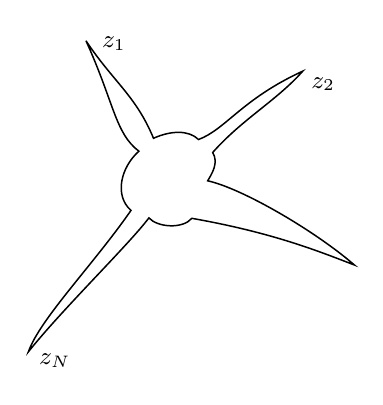
\begin{tikzpicture}[x=.0053cm,y=-.0053cm,font=\small,line width=.54pt]
\draw (154,32)..controls(219,130)and(274,164)..(316,266)
 ..controls(358,247)and(401,246)..(424,269)
 ..controls(490,244)and(528,172)..(674,105)
 ..controls(611,176)and(530,219)..(458,300)
 ..controls(473,325)and(456,351)..(446,368)
 ..controls(528,386)and(702,487)..(798,570)
 ..controls(717,539)and(606,493)..(408,458)
 ..controls(386,484)and(326,480)..(305,457)
 ..controls(255,523)and(101,672)..(16,778)
 ..controls(44,699)and(171,570)..(262,439)
 ..controls(221,403)and(238,335)..(281,297)
 ..controls(224,254)and(222,182)..(154,32);
\node[anchor=west] at (169,39) {$z_1$};
\node[anchor=west] at (671,136) {$z_2$};
\node[anchor=west] at (18,799) {$z_N$};
\end{tikzpicture}}\endgroup}
\end{GelfandAdjacentEvidence}
\begin{GelfandAdjacentEvidence}{GELFAND-P001065}{2}

\[
e^\varphi\underset{z\to z_i}{\longrightarrow}
  \frac{2}{|z-z_i|^2\log^2|z-z_i|}.
\]
хотим выч. квантовую велич.
\begin{equation*}
\Psi(z_1,\ldots,z_N)=\int\mathcal D\varphi(z)e^{-S(\varphi)}
\underset{\gamma\to0}{\simeq}e^{-S_{\mathrm{cl}}(z_1,\ldots,z_N)}.
\tag{7}
\end{equation*}
Вычислим \(S_{\mathrm{cl}}\).

(8)
\SourceFigure{GELFAND-P001065}{covering-diagram}{%
\begingroup\color{black}\GelfandFitDiagram{\begin{tikzpicture}[x=.0059cm,y=-.0059cm,font=\small,line width=.49pt]
\fill (36,175) circle [radius=3] (131,148) circle [radius=3]
 (194,206) circle [radius=3] (247,169) circle [radius=3]
 (309,155) circle [radius=2.5] (141,242) circle [radius=3];
\node at (420,196) {$\Longrightarrow$};
\node at (616,57) {$[z_1,\ldots,z_N]$};
\draw (553,235)..controls(664,247)and(817,244)..(898,246);
\draw (626,118)--(605,231)
 ..controls(621,164)and(657,150)..(660,230)
 ..controls(663,159)and(716,136)..(717,230)
 ..controls(715,168)and(777,145)..(775,228)
 ..controls(772,186)and(826,167)..(831,239)
 ..controls(839,169)and(855,136)..(864,105);
\draw (588,244)--(562,276) (641,247)--(598,289)
 (693,253)--(649,281) (756,254)--(705,288)
 (814,251)--(759,283) (860,253)--(807,286)
 (884,260)--(843,289) (899,265)--(867,294)
 (914,268)--(892,293);
\node[anchor=north] at (727,300) {(0-е углы)};
\end{tikzpicture}}\endgroup\par
Под рисунком, по-видимому, написано «0-е углы».}
\end{GelfandAdjacentEvidence}
\begin{GelfandAdjacentEvidence}{GELFAND-P001065}{3}

\SourceFigure{GELFAND-P001065}{covering-caption}{(накрывающая)}
\end{GelfandAdjacentEvidence}
\begin{GelfandAdjacentEvidence}{GELFAND-P001065}{4}


Вычислим тензор эн.-импульса:
\begin{equation*}
\begin{gathered}
T=\tfrac12(\partial_z\varphi)^2-\partial_z^2\varphi,\\
T=T_{11}-T_{22}+2iT_{12},\qquad T_{11}+T_{22}=0.
\end{gathered}
\tag{9}
\end{equation*}
(\(T_{ij}\) восстан. по \(T\), т.к. \(T_{ij}\) — вещ.)

\begin{equation*}
T(z|z_1,\ldots,z_N)
=\underset{\text{(произв. Шварца)}}{\mathcal D}[w(z)]
=\frac{w'''}{w'^2}-\frac32\frac{(w'')^2}{(w')^4}.
\tag{10}
\end{equation*}
\SourceFigure{GELFAND-P001065}{schwarzian-denominators}{В знаменателях написано \(w'^2\) и \((w')^4\).}
\end{GelfandAdjacentEvidence}
\begin{GelfandAdjacentEvidence}{GELFAND-P001065}{5}

(инвар. отн. дробно-лин. преобр.)
\[
\widetilde w(z)=\frac{\alpha w+\beta}{\gamma w+\delta}.
\]
Отсюда \(T\) — однозначна и имеет лишь полюса:
\begin{equation*}
T(z|z_1,\ldots,z_N)=\frac14\sum_1^N\frac1{(z-z_i)^2}
 +\sum_1^N\frac{c_i(z_1,\ldots,z_N)}{z-z_i}.
\tag{11}
\end{equation*}
\Unclear{GELFAND-P001065}{cancelled-pole-denominator}{Перед \(z-z_i\) в последнем знаменателе густо зачёркнута запись.}
\end{GelfandAdjacentEvidence}
\begin{GelfandAdjacentEvidence}{GELFAND-P001065}{6}


Важно, чтобы \(c_i\) были вещественны и этим \(c_i\) фиксируются.

(\(c_i\) — акцессорные коэффициенты)
\SourceFigure{GELFAND-P001065}{monodromy-insertion}{Мелко над строкой (12): «Это связ. с веществ. коэф. монодромии ур-я».}
\end{GelfandAdjacentEvidence}
\begin{GelfandAdjacentEvidence}{GELFAND-P001065}{7}


\Unclear{GELFAND-P001065}{cancelled-before-ode}{Перед (12) зачёркнута фраза, возможно «это связано».}
\end{GelfandAdjacentEvidence}
\begin{GelfandAdjacentEvidence}{GELFAND-P001065}{8}

\begin{equation*}
\psi''+T(z)\psi=0.\tag{12}
\end{equation*}
\begin{equation*}
w(z)=\frac{\psi_1(z)}{\psi_2(z)}.\tag{13}
\end{equation*}
(\(\psi_1,\psi_2\) — 2 лин. незав. реш. (13))
\SourceFigure{GELFAND-P001065}{solution-equation-reference}{В пояснении после «реш.» стоит «(13)».}
\end{GelfandAdjacentEvidence}


\uwave{Условие на вар. \(c\)}: монодромия меняется, но остаётся веществ.,

(в этом сост. задача)

(в \(\mathrm{SL}(2,\mathbb R)\), а не в \(\mathrm{SL}(2,\mathbb C)\))


\Needspace{7\baselineskip}
\begin{GelfandAdjacentEvidence}{GELFAND-P001066}{1}
\SourcePage{GELFAND-P001066}{55}
Связь:
\begin{equation*}
c_i(z_1,\ldots,z_N)=\frac{\partial S_{\mathrm{cl}}}{\partial z_i}.
\tag{14}
\end{equation*}
\SourceFigure{GELFAND-P001066}{ornament-under-fourteen}{%
\(\rule{1.45em}{.35pt}\,\boldsymbol{\cdot}\,\rule{1.7em}{.35pt}\)}
\end{GelfandAdjacentEvidence}
\begin{GelfandAdjacentEvidence}{GELFAND-P001066}{2}


Решение зад. через квантовую и затем квазиклассика при \(\gamma\to0\)!
\SourceFigure{GELFAND-P001066}{quasiclassical-parameter}{Знак при переходе к квазиклассике передан через \(\gamma\).}
\end{GelfandAdjacentEvidence}
\begin{GelfandAdjacentEvidence}{GELFAND-P001066}{3}

\begin{equation*}
[T(z_1),T(z_2)]
  =\bigl(T(z_1)+T(z_2)\bigr)\delta'(z_1-z_2)
   +\frac{c}{12}\delta'''(z_1-z_2).
\tag{15}
\end{equation*}
\Unclear{GELFAND-P001066}{eq15-superscript-correction}{Над \(z_2\) в левой части первого (15) зачёркнут небольшой знак, возможно цифра.}
\end{GelfandAdjacentEvidence}
\begin{GelfandAdjacentEvidence}{GELFAND-P001066}{4}


(завис. от \(z_1,\ldots,z_N\) не пишем)
\Unclear{GELFAND-P001066}{eq15-crossed-mark}{Перед скобкой густо зачёркнут знак.}
\end{GelfandAdjacentEvidence}
\begin{GelfandAdjacentEvidence}{GELFAND-P001066}{5}


или:
\begin{equation*}
[T(z),T(w)]
  =\bigl(T(z)+T(w)\bigr)\delta'(z-w)
   +\frac{c}{12}\delta'''(z-w)
\tag{15}
\end{equation*}
(в классике. скобки Пуассона)

Считаем:

Лагранжиан:
\[
\mathcal L=\int\bigl(\partial_z\varphi\,\partial_{\bar z}\varphi-e^\varphi\bigr)
\]
\begin{equation*}
p=\frac{\partial\mathcal L}{\partial(\partial_{\bar z}\varphi)}
  =\partial_{\bar z}\varphi
\tag{16}
\end{equation*}
\SourceFigure{GELFAND-P001066}{eq16-right-index}{В правой части (16) над нижним \(z\) видна отдельная черта.}
\end{GelfandAdjacentEvidence}
\begin{GelfandAdjacentEvidence}{GELFAND-P001066}{6}

\SourceFigure{GELFAND-P001066}{virasoro-margin}{[На правом поле] Вирасоро}
\end{GelfandAdjacentEvidence}
\begin{GelfandAdjacentEvidence}{GELFAND-P001066}{7}


откуда
\begin{equation*}
\{\varphi(z),\partial_w\varphi(w)\}=\gamma\delta(z-w).
\tag{17}
\end{equation*}
\Unclear{GELFAND-P001066}{eq17-before-delta}{Перед \(\delta\) виден отдельный знак, вероятно \(\gamma\).}
\end{GelfandAdjacentEvidence}
\begin{GelfandAdjacentEvidence}{GELFAND-P001066}{8}

\(\{T(z),T(w)\}\) и т. д.

Разлагаем в ряд Лорана:
\begin{equation*}
T(z)=\sum_n(L_n z^n+L_{-n}z^{-n})
\tag{18}
\end{equation*}
\begin{equation*}
[L_n,L_m]=(n-m)L_{n+m}+\frac{c}{12}n(n^2-1),
\quad c=26-D.
\tag{19}
\end{equation*}
\SourceFigure{GELFAND-P001066}{eq19-central-term}{После \(n(n^2-1)\) в (19) стоит запятая.}
\end{GelfandAdjacentEvidence}
\begin{GelfandAdjacentEvidence}{GELFAND-P001066}{9}

(можно было предсказать из рез. Гельфанда–Фукса из вида центр. расш.)

\[
\widetilde z=z+\varepsilon(z)\qquad\text{(вариация)}
\]
\[
\delta\varphi=\operatorname{Re}
  \bigl(\varepsilon(z)\partial_z\varphi+\partial_z\varepsilon\bigr)
\]
К действию доб. число \(\rightsquigarrow\) появл. центр. расширение).
\SourceFigure{GELFAND-P001066}{central-extension-arrow}{Между двумя фразами проведена волнистая стрелка.}
\end{GelfandAdjacentEvidence}
\begin{GelfandAdjacentEvidence}{GELFAND-P001066}{10}


Попробуем найти \(\Psi\) чисто алгебраически:
\begin{equation*}
\text{Пусть}\qquad T_\varepsilon=\int\varepsilon(z)T(z)\,d^2z
\tag{20}
\end{equation*}
\SourceFigure{GELFAND-P001066}{shift-generator}{%
\(\longleftarrow\) Предположим, что генератор сдвига.}
\end{GelfandAdjacentEvidence}
\begin{GelfandAdjacentEvidence}{GELFAND-P001066}{11}

\begin{equation*}
\delta_\varepsilon\psi=[T_\varepsilon,\psi(z)]
 =\varepsilon(z)\frac{d\psi}{dz}+\Delta\cdot\varepsilon'(z)\psi(z)
\tag{21}
\end{equation*}
(вариация поля \(\psi\))
\begin{equation*}
[L_n,\psi(z)]
 =z^{n+1}\frac{d\psi}{dz}+(n+1)\Delta\psi(z).
\tag{22}
\end{equation*}
\SourceFigure{GELFAND-P001066}{eq22-weight-term}{Второе слагаемое (22) читается \((n+1)\Delta\psi(z)\).}
\end{GelfandAdjacentEvidence}


\(\psi(z)\) — опер. в том же пр-ве, где задано представление.


\Needspace{7\baselineskip}
\begin{GelfandAdjacentEvidence}{GELFAND-P001067}{1}
\SourcePage{GELFAND-P001067}{unlabelled}
$\psi(z)$ — опер. рожд. рога на сфере.
\begin{equation*}
\Psi(z)|v\rangle.
\end{equation*}
\SourceFigure{GELFAND-P001067}{initial-ket-glyph}{Прописное начертание $\Psi$ в строке с кетом.}
\end{GelfandAdjacentEvidence}
\begin{GelfandAdjacentEvidence}{GELFAND-P001067}{2}

Рассм. ф-и:
\begin{equation*}
\langle v|\psi(z_1)\psi(z_2)\psi(z_3)\psi(z_4)|v\rangle
\tag{23}
\end{equation*}
\begin{equation*}
\Psi(x)=\langle v|\psi(\infty)\psi(1)\psi(x)\psi(0)|v\rangle
\end{equation*}
\begin{equation*}
|0\rangle=\psi(0)|v\rangle,\qquad \langle v|\psi(\infty)=\langle0|
\end{equation*}
\SourceFigure{GELFAND-P001067}{overwritten-bra}{Угловая скобка бра обведена.}
\end{GelfandAdjacentEvidence}
\begin{GelfandAdjacentEvidence}{GELFAND-P001067}{3}

\begin{equation*}
\Psi(x)=\langle0|\psi(1)\psi(x)|0\rangle
\end{equation*}
\begin{equation*}
\begin{cases}
L_n|0\rangle=0,\quad n>0,\\
L_0|0\rangle=\Delta|0\rangle
\end{cases}
\tag{24}
\end{equation*}
Возникают модули Верма: такое предст. без лишних соотн.

$\psi(x)$ (возможно, $\Psi(x)$), знак переправлен\textsuperscript{?} опис. выше и перев. мод. Верма в себя.
\Unclear{GELFAND-P001067}{overwritten-field}{$\psi(x)$ (возможно, $\Psi(x)$), знак переправлен}
\end{GelfandAdjacentEvidence}
\begin{GelfandAdjacentEvidence}{GELFAND-P001067}{4}

\begin{equation*}
\Psi(x)=e^{\Delta\cdot S_{cl}(x)}\quad\Rightarrow\quad\text{по \(\Psi(x)\) всё опред.}
\tag{25}
\end{equation*}
зачёркнутый знак, возможно § или 4\textsuperscript{?}\ \uwave{Вычисление $\Psi$.}
\Unclear{GELFAND-P001067}{heading-mark}{зачёркнутый знак, возможно § или 4}
\end{GelfandAdjacentEvidence}
\begin{GelfandAdjacentEvidence}{GELFAND-P001067}{5}


Добавим соотношение (к коммут. соотн.):
\begin{equation*}
\langle0|\psi(x)|0\rangle=x^{-\Delta}
\tag{26}
\end{equation*}
\begin{equation*}
\begin{aligned}
&\langle0|\psi(1)|0\rangle\langle0|\psi(x)|0\rangle+
\langle0|\psi(1)|1\rangle\langle1|\psi(x)|0\rangle+\\
&\quad+\langle0|\psi(1)|2\rangle\langle2|\psi(x)|0\rangle+\ldots
\end{aligned}
\tag{27}
\end{equation*}
\begin{equation*}
I=\sum_n|n\rangle\langle n|
\end{equation*}
\begin{equation*}
\begin{aligned}
\langle1|\psi(x)|0\rangle
&=\langle0|L_1\psi(x)|0\rangle
=\langle0|[L_1,\psi(x)]|0\rangle=\\
&=\left(x^2\frac{d}{dx}+2\Delta x\right)\langle0|\psi(x)|0\rangle
=(\Delta\cdot x)x^{-\Delta}
\end{aligned}
\end{equation*}
[после \(2\Delta\) запись зачёркнута, вписано \(x\). Под строкой знак вставки или \(y\)\textsuperscript{?}]
\Unclear{GELFAND-P001067}{matrix-element-correction}{после \(2\Delta\) запись зачёркнута, вписано \(x\). Под строкой знак вставки или \(y\)}
\end{GelfandAdjacentEvidence}
\begin{GelfandAdjacentEvidence}{GELFAND-P001067}{6}


и далее получается:
\begin{equation*}
\psi(x)=x^{-\Delta}\left\{1+\frac{\Delta}{2}x+\ldots\right\}
\end{equation*}
\SourceFigure{GELFAND-P001067}{series-glyph}{Строчное начертание $\psi$ в разложении.}
\end{GelfandAdjacentEvidence}
\begin{GelfandAdjacentEvidence}{GELFAND-P001067}{7}

\begin{equation*}
\langle v|\psi(z_1)\ldots\psi(z_N)|v\rangle=e^{-S_{ii}(z_1,\ldots,z_N)}
\end{equation*}
[нижний индекс у \(S\), вероятно \(ii\), возможно \(il\)\textsuperscript{?}]
\Unclear{GELFAND-P001067}{action-subscript}{нижний индекс у \(S\), вероятно \(ii\), возможно \(il\)}
\end{GelfandAdjacentEvidence}
\begin{GelfandAdjacentEvidence}{GELFAND-P001067}{8}

\begin{equation*}
\Delta,c\to\infty
\end{equation*}
$c_i(z_1,\ldots,z_N)$ при $z_i-z_j\to0$ [зачёркнуто «пр…». Знак между \(z_i\) и \(z_j\) обведён, читается как минус\textsuperscript{?}] перех. в предыдущий акцессорный коэффициент?
\Unclear{GELFAND-P001067}{last-line-cancellation}{зачёркнуто «пр…». Знак между \(z_i\) и \(z_j\) обведён, читается как минус}
\end{GelfandAdjacentEvidence}



\Needspace{7\baselineskip}
\begin{GelfandAdjacentEvidence}{GELFAND-P001068}{1}
\SourcePage{GELFAND-P001068}{56}
$S_{cl}(x)$

(3 другие точки $0,1,\infty$)

\sout{Остальные} $\Rightarrow c_k=c_k(x)$
\SourceFigure{GELFAND-P001068}{deleted-word}{Зачёркнутое слово.}
\end{GelfandAdjacentEvidence}
\begin{GelfandAdjacentEvidence}{GELFAND-P001068}{2}

\begin{equation*}
c_k(x)=\frac{\partial S_{cl}(x)}{\partial x}
\end{equation*}
\begin{equation*}
e^{S_{cl}(x)}=x^{-\Delta}\{1+a_1x+a_2x^2+\ldots\}.
\end{equation*}
[заштрихованная запись в показателе после \(S_{cl}(x)\)\textsuperscript{?}]
\Unclear{GELFAND-P001068}{exponent-cancelled-mark}{заштрихованная запись в показателе после \(S_{cl}(x)\)}
\end{GelfandAdjacentEvidence}
\begin{GelfandAdjacentEvidence}{GELFAND-P001068}{3}

\uwave{коэфф. $a_j$ вычисл. с пом. алгебры.}
\SourceFigure{GELFAND-P001068}{coefficient-underlining}{Волнистое подчёркивание и две короткие черты ниже.}
\end{GelfandAdjacentEvidence}
\begin{GelfandAdjacentEvidence}{GELFAND-P001068}{4}


Аксиомы:
\begin{equation*}
L_0|0\rangle=\Delta|0\rangle
\end{equation*}
\begin{equation*}
L_n|0\rangle=0,\quad n>0
\end{equation*}
\begin{equation*}
[L_n,\psi(x)]=\left(x^{n+1}\frac{d}{dx}+(n+1)\Delta\right)\psi(x)
\end{equation*}
\SourceFigure{GELFAND-P001068}{axiom-commutator}{Рукописная запись коммутатора. Множитель \(x^n\) при \((n+1)\Delta\) в этой строке отсутствует.}
\end{GelfandAdjacentEvidence}
\begin{GelfandAdjacentEvidence}{GELFAND-P001068}{5}

\begin{equation*}
\langle0|\psi(x)|0\rangle=x^{-\Delta}
\end{equation*}
\begin{equation*}
\Psi(x)=\langle0|\psi(1)\psi(x)|0\rangle
\end{equation*}
[неразборчивый зачёркнутый знак после кета]
\Unclear{GELFAND-P001068}{correlator-end-mark}{неразборчивый зачёркнутый знак после кета}
\end{GelfandAdjacentEvidence}
\begin{GelfandAdjacentEvidence}{GELFAND-P001068}{6}

\begin{equation*}
I=\sum_n|n\rangle\langle n|,\qquad |n\rangle=L_{-n}|0\rangle.
\end{equation*}
[На левом поле: $\psi(x)$ — ?]
\SourceFigure{GELFAND-P001068}{field-margin}{Запись на левом поле.}
\end{GelfandAdjacentEvidence}
\begin{GelfandAdjacentEvidence}{GELFAND-P001068}{7}


Сложность. нет ортогональности.

Из вида $T$ естественно:
\begin{equation*}
L_n=(\alpha+i\beta n)a_n+\sum_{k=1}^{n-1}a_ka_{n-k}+\sum_{k=1}^{\infty}a_k^+a_{n+k};
\end{equation*}
\begin{equation*}
L_{-n}=L_n^+;
\end{equation*}
\begin{equation*}
[a_n,a_m^+]=n\delta_{n,m};
\end{equation*}
\begin{equation*}
\Delta=\frac12(\alpha^2+\beta^2),\quad c=1+12\beta^2.
\end{equation*}
\begin{equation*}
a_n|0\rangle=0.
\end{equation*}
Есть соотв. базисов:
\begin{equation*}
a_{n_1}^+a_{n_2}^+\ldots|0\rangle
\end{equation*}
[неразборчивый зачёркнутый знак справа от первой строки базиса]
\Unclear{GELFAND-P001068}{first-basis-end-mark}{неразборчивый зачёркнутый знак справа от первой строки базиса}
\end{GelfandAdjacentEvidence}

\begin{equation*}
L_{-n_1}L_{-n_2}\ldots|0\rangle
\end{equation*}
выр. друг через друга, но 1-й ортогонален!!

Коммут. соотн. $\psi(x)$ в 1-м баз. сложнее
\begin{equation*}
L(z)=T(z)=\frac{dp(z)}{dz}+p^2(z),
\end{equation*}
где
\begin{equation*}
p(z)=\sum(a_nz^n+a_{-n}z^{-n})
\end{equation*}


\Needspace{7\baselineskip}
\begin{GelfandAdjacentEvidence}{GELFAND-P001069}{1}
\SourcePage{GELFAND-P001069}{unlabelled}
Считаем $a_n=\dfrac{\partial}{\partial z_n}$, $a_n^+=nz_n$.
\begin{equation*}
\begin{aligned}
&(\alpha+i\beta n)\frac{\partial}{\partial z_n}
+\sum\frac{\partial^2}{\partial z_k\partial z_{n-k}}
+\sum kz_k\frac{\partial}{\partial z_{n+k}}\biggr)
F(x,z_1,z_2,\ldots,\,) =\\
&\qquad=\left(x^{n+1}\frac{\partial}{\partial x}+(n+1)\Delta\right)F(x,z_1,\, ,z_n).
\end{aligned}
\end{equation*}
[слева \(F\) написано поверх другого знака. Нижний знак неразборчив]
\Unclear{GELFAND-P001069}{lhs-function-overwrite}{слева \(F\) написано поверх другого знака. Нижний знак неразборчив}
\end{GelfandAdjacentEvidence}
\begin{GelfandAdjacentEvidence}{GELFAND-P001069}{2}

\SourceFigure{GELFAND-P001069}{function-argument-gaps}{Аргументы слева. Запятая примыкает к \(z_1\), после последней запятой оставлен пробел.}
\end{GelfandAdjacentEvidence}
\begin{GelfandAdjacentEvidence}{GELFAND-P001069}{3}

\SourceFigure{GELFAND-P001069}{function-argument-gaps-rhs}{Аргументы справа с пробелом между запятыми.}
\end{GelfandAdjacentEvidence}
\begin{GelfandAdjacentEvidence}{GELFAND-P001069}{4}

\SourceFigure{GELFAND-P001069}{differential-operator-notation}{Начало левой части. Перед первой скобкой нет отдельной внешней открывающей скобки.}
\end{GelfandAdjacentEvidence}
\begin{GelfandAdjacentEvidence}{GELFAND-P001069}{5}

\SourceFigure{GELFAND-P001069}{differential-operator-rhs-factor}{Правая часть. При \((n+1)\Delta\) множитель \(x^n\) не написан.}
\end{GelfandAdjacentEvidence}



\Needspace{7\baselineskip}
\begin{GelfandAdjacentEvidence}{GELFAND-P001070}{1}
\SourcePage{GELFAND-P001070}{unlabelled}
\uuline{29/XI–82 г.} \uline{Сем. Гельфанда.}

\uline{Кобзарев} (Игорь Юрьевич)

\uline{О струнах.}
\SourceFigure{GELFAND-P001070}{speaker-heading}{Дата, имя докладчика и заглавие.}
\end{GelfandAdjacentEvidence}
\begin{GelfandAdjacentEvidence}{GELFAND-P001070}{2}


\dashuline{Теория поля}: есть поле $\varphi$, $M^4$ — пр-во Минк., $\mathcal L(\varphi)$ — лагранжиан.

реш. и т. п.

\dashuline{Другой тип теор. поля}

до 1970 г.
\begin{equation*}
\Box\psi+\mu^2\psi=0
\tag{1}
\end{equation*}
\SourceFigure{GELFAND-P001070}{mass-symbol}{Запись \(\mu^2\) в (1).}
\end{GelfandAdjacentEvidence}
\begin{GelfandAdjacentEvidence}{GELFAND-P001070}{3}

[Справа:] Взаимод. — теор. возмущ. $\varphi_1\varphi_2\varphi_3$, $\ldots$

надо доб. $\lambda\varphi_1\varphi_2\varphi_3$ и т. д.

после: \dashuline{Хиггсовского типа}
\SourceFigure{GELFAND-P001070}{higgs-heading}{Рукописная строка «после: Хиггсовского типа».}
\end{GelfandAdjacentEvidence}
\begin{GelfandAdjacentEvidence}{GELFAND-P001070}{4}

\begin{equation*}
\mathcal{L}(\varphi)=\frac12(\partial_i\varphi)^2-\lambda^2(\varphi^2-\eta^2)^2
\tag{2}
\end{equation*}
Вакуум: на клас. полях — сост. с наименьшей энергией \(\parallel\)
\SourceFigure{GELFAND-P001070}{vacuum-margin}{Двойная черта справа от строки о вакууме.}
\end{GelfandAdjacentEvidence}
\begin{GelfandAdjacentEvidence}{GELFAND-P001070}{5}


(соотв. гамильтониан:
\begin{equation*}
H=\frac12(\partial_t\varphi)^2+\frac12(\bar\nabla\varphi)^2+\lambda^2(\varphi^2-\eta^2)^2
\tag{3}
\end{equation*}
\SourceFigure{GELFAND-P001070}{hamiltonian-number}{Обведённая повторным штрихом цифра 3.}
\end{GelfandAdjacentEvidence}
\begin{GelfandAdjacentEvidence}{GELFAND-P001070}{6}

\SourceFigure{GELFAND-P001070}{hamiltonian-gradient}{Черта над \(\nabla\) в (3).}
\end{GelfandAdjacentEvidence}
\begin{GelfandAdjacentEvidence}{GELFAND-P001070}{7}


\dashuline{Вырожд. вакуум}: $\varphi=\eta$, $\varphi=-\eta$. (2 вакуума)
\begin{equation*}
\varphi\mapsto-\varphi\qquad\text{дискр. симм.}
\tag{4}
\end{equation*}
\SourceFigure{GELFAND-P001070}{domain-wall-diagram}{%
\begin{center}
\begingroup\color{black}\GelfandFitDiagram{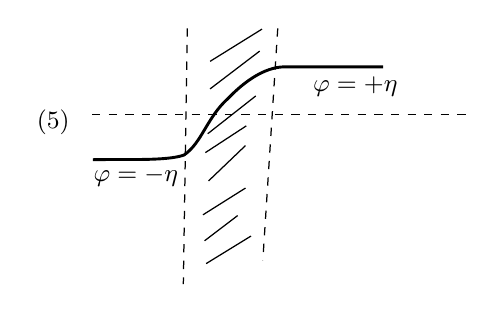
\begin{tikzpicture}[x=.010cm,y=-.010cm,font=\small,line width=.45pt]
\node[anchor=east] at (-16,119) {(5)};
\draw[dashed] (0,110)--(476,110);
\draw[dashed] (121,0)--(116,325) (236,0)--(217,295);
\draw (150,42)--(216,1) (150,77)--(213,29) (147,134)--(208,86)
      (144,158)--(196,124) (148,194)--(195,149) (141,237)--(195,203)
      (143,270)--(185,238) (145,299)--(202,264);
\draw[line width=1.05pt] (1,167)..controls(42,166)and(95,169)..(117,161)
 ..controls(140,145)and(146,113)..(173,89)
 ..controls(194,67)and(219,50)..(243,49)--(370,49);
\node[anchor=north east,inner sep=0pt] at (110,175) {$\varphi=-\eta$};
\node[anchor=north west,inner sep=0pt] at (280,61) {$\varphi=+\eta$};
\end{tikzpicture}}\endgroup
\end{center}}
\end{GelfandAdjacentEvidence}
\begin{GelfandAdjacentEvidence}{GELFAND-P001070}{8}

[Справа от рисунка:] Рассм. стенку — \uwave{реш., локализ. на плоскости.}
\begin{equation*}
\varphi=\varphi(x,y,z)\qquad(\text{не зав. от \(t\)})
\end{equation*}
\begin{equation*}
\Box\varphi+\varphi\lambda^2(\varphi^2-\eta^2)=0
\qquad\text{— ур-е Эйлера для лагр. (2)}
\tag{6}
\end{equation*}
\SourceFigure{GELFAND-P001070}{eq06-coefficient}{Перед \(\lambda^2\) написано \(\varphi\).}
\end{GelfandAdjacentEvidence}
\begin{GelfandAdjacentEvidence}{GELFAND-P001070}{9}


(7) $\parallel\quad\underset{z\to\pm\infty}{\varphi=\pm\eta}$
от $x,y,z$ не зависит $\Rightarrow$ легко пров., что такое реш. сущ.
\SourceFigure{GELFAND-P001070}{limit-coordinate-reading}{Условие на бесконечности и перечень координат в рукописи.}
\end{GelfandAdjacentEvidence}



\Needspace{7\baselineskip}
\begin{GelfandAdjacentEvidence}{GELFAND-P001071}{1}
\SourcePage{GELFAND-P001071}{unlabelled}
$\eta\sim m$

(8) Толщина слоя [вставлено снизу: (в (5))] $\sim\dfrac1\eta$.
\SourceFigure{GELFAND-P001071}{thickness-insertion}{Ссылка на (5) под строкой о толщине слоя.}
\end{GelfandAdjacentEvidence}
\begin{GelfandAdjacentEvidence}{GELFAND-P001071}{2}


[неразборчивый зачёркнутый знак перед «Реш.»] Реш. (5) явно нах.: \uuline{$\operatorname{th}(z\eta)$}
\Unclear{GELFAND-P001071}{before-solution05}{неразборчивый зачёркнутый знак перед «Реш.»}
\end{GelfandAdjacentEvidence}
\begin{GelfandAdjacentEvidence}{GELFAND-P001071}{3}

\SourceFigure{GELFAND-P001071}{explicit-wall-solution}{Дважды подчёркнутое \(\operatorname{th}(z\eta)\).}
\end{GelfandAdjacentEvidence}
\begin{GelfandAdjacentEvidence}{GELFAND-P001071}{4}


\dashuline{Гр. симметрии}: $\varphi\mapsto-\varphi$.

Сейчас обычно рассм. непр. гр. $G$ симм. лагранжиана.
\SourceFigure{GELFAND-P001071}{continuous-symmetry}{Сокращения в строке о непрерывной группе.}
\end{GelfandAdjacentEvidence}
\begin{GelfandAdjacentEvidence}{GELFAND-P001071}{5}


$U(1)$-инвар. теория:
\begin{equation*}
\mathcal{L}(\varphi)=\frac12\bigl|(\partial_i+iA_i)\varphi\bigr|^2-(\varphi\varphi^*-\eta^2)^2
\tag{9}
\end{equation*}
\SourceFigure{GELFAND-P001071}{covariant-derivative-sign}{Знак \(+\) перед \(iA_i\) в (9).}
\end{GelfandAdjacentEvidence}
\begin{GelfandAdjacentEvidence}{GELFAND-P001071}{6}

\begin{equation*}
\text{Вакуум: }(c_1,c_2):\quad c_1^2+c_2^2=\eta^2
\tag{10}
\end{equation*}
\SourceFigure{GELFAND-P001071}{diagram11}{%
\begin{center}
\begingroup\color{black}\GelfandFitDiagram{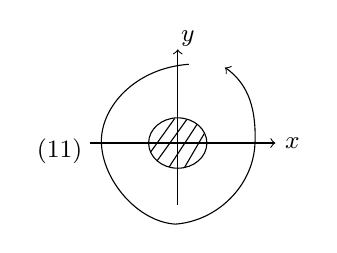
\begin{tikzpicture}[x=1cm,y=1cm,font=\small]
\node at (-1.50,-.11) {(11)};
\draw[->] (-1.12,0)--(1.24,0) node[right] {$x$};
\draw[->] (0,-.79)--(0,1.19) node[above right,inner sep=1pt] {$y$};
\draw (0,0) ellipse [x radius=.37,y radius=.32];
\begin{scope}
\clip (0,0) ellipse [x radius=.37,y radius=.32];
\draw (-.37,-.15)--(-.04,.31) (-.33,-.32)--(.13,.32)
      (-.12,-.32)--(.26,.26) (.08,-.32)--(.36,.16);
\end{scope}
\draw[->] (.14,1.00)..controls(-.55,.95)and(-.98,.45)..(-.97,.01)
 ..controls(-.96,-.47)and(-.51,-1.00)..(-.03,-1.03)
 ..controls(.50,-.99)and(.95,-.55)..(.98,-.02)
 ..controls(1.00,.41)and(.91,.74)..(.60,.96);
\end{tikzpicture}}\endgroup
\end{center}}
\end{GelfandAdjacentEvidence}
\begin{GelfandAdjacentEvidence}{GELFAND-P001071}{7}

[Справа от рисунка:] струна: когда энергия соср. на линии (1-мерной).

При обходе вектор $C$ поворач. на $2\pi$

Топологич. инвариант есть.

(Статическое решение: не зав. от $t$)

$A$ — доп. вект. поле (эл.-магн.)
\begin{equation*}
\mathcal{L}=-\frac14F_{ik}F_{ik}+\frac12\bigl|(\partial_i+iA_i)\varphi\bigr|^2-(\varphi\varphi^*-\eta^2)^2
\tag{12}
\end{equation*}
\begin{equation*}
F_{ik}=\partial_i A_k-\partial_k A_i
\end{equation*}
Действие $U(1)$ на поле:
\begin{equation*}
\begin{cases}
\varphi\mapsto e^{i\alpha}\varphi\\
A_i\mapsto A_i+\nabla_i\alpha
\end{cases}
\tag{13}
\end{equation*}
\SourceFigure{GELFAND-P001071}{eq13-gauge-sign}{В (13) написаны \(e^{i\alpha}\) и знак \(+\) перед \(\nabla_i\alpha\).}
\end{GelfandAdjacentEvidence}
\begin{GelfandAdjacentEvidence}{GELFAND-P001071}{8}


Рассм. приближ. решение [зачёркнутая запись, возможно номер в скобках\textsuperscript{?}]
\Unclear{GELFAND-P001071}{after-approximate-solution}{зачёркнутая запись, возможно номер в скобках}
\end{GelfandAdjacentEvidence}
\begin{GelfandAdjacentEvidence}{GELFAND-P001071}{9}


\SourceFigure{GELFAND-P001071}{diagram14}{%
\begin{center}
\begingroup\color{black}\GelfandFitDiagram{\begin{tikzpicture}[x=.010cm,y=-.010cm,font=\small,line width=.55pt]
\node at (5,189) {(14)};
\draw (291,0)..controls(273,66)and(281,104)..(237,133)
 ..controls(192,158)and(177,175)..(179,214)
 ..controls(177,260)and(227,277)..(234,319)
 ..controls(242,365)and(227,467)..(218,539);
\draw (305,3)..controls(302,80)and(280,136)..(254,162)
 ..controls(230,188)and(202,177)..(207,214)
 ..controls(209,253)and(249,284)..(251,326)
 ..controls(264,380)and(242,494)..(239,533);
\draw[line width=.83pt] (237,133)--(254,162) (196,158)--(215,185);
\draw (201,160)--(234,140) (206,168)--(238,146)
      (211,175)--(242,153) (215,181)--(246,159);
\draw (284,50)--(303,46) (280,82)--(296,80) (251,119)--(279,117)
      (189,174)--(199,171) (186,211)--(204,206) (191,244)--(205,239)
      (207,264)--(222,264) (222,289)--(235,287) (235,309)--(250,310)
      (237,347)--(250,344) (235,380)--(251,380) (232,415)--(249,412)
      (228,451)--(245,449) (226,477)--(242,474) (221,506)--(238,503);
\draw[->] (441,225)..controls(374,222)and(285,203)..(220,194);
\node at (337,249) {$r_{\text{кр}}$};
\draw[->,line width=.80pt] (457,120)--(386,129);
\end{tikzpicture}}\endgroup
\end{center}
Подпись к стрелке у перегиба читается \(r_{\text{кр}}\). В выделенном участке возможны наконечники штрихов.}
\end{GelfandAdjacentEvidence}
\begin{GelfandAdjacentEvidence}{GELFAND-P001071}{10}

[Справа от рисунка, стрелка влево:] \uwave{примем это за начальное условие}
\SourceFigure{GELFAND-P001071}{initial-condition-caption}{Волнистое подчёркивание и единственное число в словах «начальное условие».}
\end{GelfandAdjacentEvidence}
\begin{GelfandAdjacentEvidence}{GELFAND-P001071}{11}


Примерн. вид решения (11):
\begin{equation*}
\begin{cases}
\varphi_1=\dfrac xr f(r)\\
\varphi_2=\dfrac yr f(r)
\end{cases}
\tag{15}
\end{equation*}
(для вероятно «поворота», начальные буквы различимы не полностью\textsuperscript{?})
\Unclear{GELFAND-P001071}{eq15-parenthesis-word}{вероятно «поворота», начальные буквы различимы не полностью}
\end{GelfandAdjacentEvidence}


[Справа:] так же конструир. $A$

$\varepsilon(r)$ — плотность энергии в (11) — вычисляется.


\Needspace{7\baselineskip}
\begin{GelfandAdjacentEvidence}{GELFAND-P001072}{1}
\SourcePage{GELFAND-P001072}{67}
[Зачёркнуто: возможно «Решение (14)»\textsuperscript{?}]
\Unclear{GELFAND-P001072}{top-cancelled-reference}{возможно «Решение (14)»}
\end{GelfandAdjacentEvidence}
\begin{GelfandAdjacentEvidence}{GELFAND-P001072}{2}


Должны вых. на вакуум: $\varphi_1^2+\varphi_2^2\to\eta^2$ при $r\to\infty$.

Локально (14) похоже на (11).

(16) Пусть радиус кривизны $r_{\text{кр}}\gg\dfrac1\eta$

Эфф. действие: [стрелка вправо, затем вниз к правой части (17)]
\begin{equation*}
S=\int\mathcal L(\varphi)\,d^4x\simeq\nu\int dl\sqrt{1-v_{\perp}^2}\,dt
\tag{17}
\end{equation*}
[Справа сверху, стрелка влево-вниз к интегралу:] интеграл по самой струне.
\SourceFigure{GELFAND-P001072}{effective-action-arrows}{Две стрелки к правой части (17).}
\end{GelfandAdjacentEvidence}
\begin{GelfandAdjacentEvidence}{GELFAND-P001072}{3}

\SourceFigure{GELFAND-P001072}{action-density-symbol}{Коэффициент \(\nu\) перед интегралом в (17).}
\end{GelfandAdjacentEvidence}
\begin{GelfandAdjacentEvidence}{GELFAND-P001072}{4}


$v_\perp$ — поперечная скор. струны

\(\parallel\) $\nu$ — линейная плотность энергии струны.
\SourceFigure{GELFAND-P001072}{linear-density-key}{Двойная черта и пояснение к \(\nu\).}
\end{GelfandAdjacentEvidence}
\begin{GelfandAdjacentEvidence}{GELFAND-P001072}{5}


Эволюция — ?

Внутри струны счит., [вставлено сверху: что] ничего не происходит
\SourceFigure{GELFAND-P001072}{inside-string-insertion}{Над строкой вписано «что».}
\end{GelfandAdjacentEvidence}
\begin{GelfandAdjacentEvidence}{GELFAND-P001072}{6}

(счит. [вставлено сверху: толщину] её дост. малой — — по сравнению с радиусами кривизны)
\SourceFigure{GELFAND-P001072}{thickness-insertion}{Вставка «толщину» перед «её».}
\end{GelfandAdjacentEvidence}
\begin{GelfandAdjacentEvidence}{GELFAND-P001072}{7}


Интеграл вычисляем в каждом трансверс. сечении — получим $\nu$

$\sqrt{1-v_\perp^2}$ получается из $d^4x$ (заменой переменных)

Или: воспольз. релятивистской инвар.: $ds$ (интервал), запис. в $\forall$ сист. координат.

(17) — ф-ла \uline{Намбу́}.

Можно рассм. кольцевую струну с лагранж. — пр. часть (17)
\SourceFigure{GELFAND-P001072}{diagram18}{%
\begin{center}
\begingroup\color{black}\GelfandFitDiagram{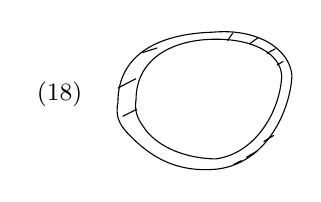
\begin{tikzpicture}[x=1cm,y=1cm,font=\small]
\node at (-1.86,.10) {(18)};
\draw (-1.12,.00)..controls(-1.12,.59)and(-.63,.87)..(.09,.89)
 ..controls(.65,.94)and(1.06,.68)..(1.09,.34)
 ..controls(1.07,-.10)and(.77,-.78)..(.13,-.85)
 ..controls(-.42,-.90)and(-.75,-.65)..(-.98,-.41)
 ..controls(-1.12,-.27)and(-1.15,-.16)..cycle;
\draw (-.89,.03)..controls(-.89,.54)and(-.45,.79)..(.09,.80)
 ..controls(.59,.81)and(.95,.62)..(.96,.33)
 ..controls(.94,-.10)and(.64,-.65)..(.12,-.72)
 ..controls(-.34,-.71)and(-.66,-.52)..(-.79,-.32)
 ..controls(-.88,-.20)and(-.91,-.10)..cycle;
\draw (-1.12,.18)--(-.89,.30) (-1.06,-.18)--(-.88,-.09)
 (-.81,.63)--(-.62,.69) (.34,.88)--(.27,.78)
 (.66,.82)--(.55,.74) (.88,.68)--(.77,.62)
 (.98,.52)--(.90,.47) (.86,-.42)--(.73,-.50)
 (.65,-.62)--(.51,-.70) (.45,-.74)--(.35,-.79);
\end{tikzpicture}}\endgroup
\end{center}}
\end{GelfandAdjacentEvidence}
\begin{GelfandAdjacentEvidence}{GELFAND-P001072}{8}

оно будет сжиматься, быстро вых. на световую скорость и сжимается в комочек.

\dashuline{Вариант.}

обрыв концов (сажаем на них по монополю):
\SourceFigure{GELFAND-P001072}{diagram19}{%
\begin{center}
\begingroup\color{black}\GelfandFitDiagram{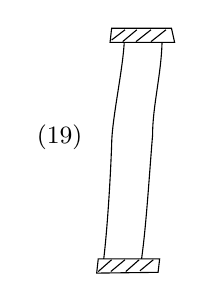
\begin{tikzpicture}[x=1cm,y=1cm,font=\small]
\node at (-1.00,.15) {(19)};
\draw (-.18,1.35)..controls(-.20,.98)and(-.34,.36)..(-.34,.04)
 ..controls(-.36,-.49)and(-.40,-1.06)..(-.44,-1.40);
\draw (.30,1.35)..controls(.29,.94)and(.18,.54)..(.18,.17)
 ..controls(.14,-.31)and(.10,-.98)..(.04,-1.40);
\draw (-.36,1.35)--(.46,1.35)--(.42,1.53)--(-.34,1.53)--cycle;
\draw (-.53,-1.58)--(.25,-1.57)--(.27,-1.40)--(-.51,-1.40)--cycle;
\draw (-.34,1.38)--(-.17,1.51) (-.20,1.36)--(-.02,1.51)
 (-.03,1.36)--(.16,1.51) (.16,1.36)--(.35,1.51)
 (-.51,-1.56)--(-.34,-1.41) (-.35,-1.56)--(-.17,-1.41)
 (-.16,-1.56)--(.01,-1.41) (.02,-1.55)--(.19,-1.41);
\end{tikzpicture}}\endgroup
\end{center}}
\end{GelfandAdjacentEvidence}
\begin{GelfandAdjacentEvidence}{GELFAND-P001072}{9}

\SourceFigure{GELFAND-P001072}{diagram20}{%
\begin{center}
\begingroup\color{black}\GelfandFitDiagram{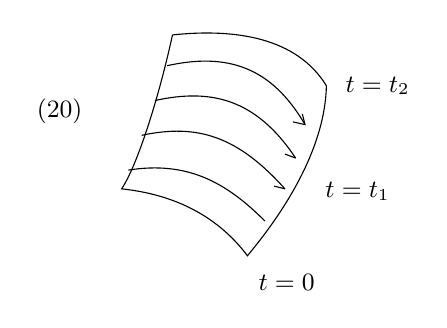
\begin{tikzpicture}[x=.017cm,y=-.017cm,font=\small]
\node[anchor=east] at (-22,57) {(20)};
\draw (38,0)..controls(85,-5)and(131,2)..(153,38)
 ..controls(152,83)and(124,129)..(94,165)
 ..controls(76,141)and(47,120)..(0,115)
 ..controls(12,97)and(28,46)..(38,0);
\draw (34,23)..controls(79,13)and(112,24)..(137,67)
 (25,49)..controls(66,40)and(100,47)..(130,92)
 (15,75)..controls(57,66)and(87,76)..(122,115)
 (5,101)..controls(49,94)and(78,110)..(107,139);
\draw (128,65)--(137,67)--(135,59)
 (122,89)--(130,92) (114,113)--(122,115);
\node[anchor=west] at (160,38) {$t=t_2$};
\node[anchor=west] at (145,117) {$t=t_1$};
\node[anchor=north west] at (95,172) {$t=0$};
\end{tikzpicture}}\endgroup
\end{center}
Короткие ответвления видны на концах трёх дуг. Их смысл как наконечников не вполне ясен.}
\end{GelfandAdjacentEvidence}
\begin{GelfandAdjacentEvidence}{GELFAND-P001072}{10}


[Справа от рисунка:] при движении струна заметает пластину.

(21) \uwave{Площадь заметаемой поверхности и есть лагранжиан} ($17_{\text{пр}}$)
\SourceFigure{GELFAND-P001072}{swept-area-caption}{Волнистое подчёркивание и ссылка \(17_{\text{пр}}\).}
\end{GelfandAdjacentEvidence}



\Needspace{7\baselineskip}
\begin{GelfandAdjacentEvidence}{GELFAND-P001073}{1}
\SourcePage{GELFAND-P001073}{unlabelled}
$\dot x=\dfrac{\partial x}{\partial t}$, $x'=\dfrac{\partial x}{\partial s}$, $x(t,s)$ и считаем.

Возникает $\min$ площадь.
\SourceFigure{GELFAND-P001073}{minimum-area-ending}{Слово после \(\min\) оканчивается на «ь».}
\end{GelfandAdjacentEvidence}
\begin{GelfandAdjacentEvidence}{GELFAND-P001073}{2}


\uwave{Струны и хромодинамика.}

\dashuline{Квант. хромодинамика}:
\begin{equation*}
\mathcal L(\psi,A)=-\frac14F_{ik}^aF_{ik}^a+\bar\psi(i\hat\partial-m)\psi
\tag{22}
\end{equation*}
\SourceFigure{GELFAND-P001073}{eq22-field-case}{Строчные \(\psi\) в правой части (22).}
\end{GelfandAdjacentEvidence}
\begin{GelfandAdjacentEvidence}{GELFAND-P001073}{3}


$a=1\div8$; $i,k=0,1,2,3$.
\begin{equation*}
\hat\partial=\gamma^i(\partial_i+iI^aA_i^a)
\tag{23}
\end{equation*}
[Под $\gamma^i$:] матр. Дирака
\SourceFigure{GELFAND-P001073}{dirac-matrix-caption}{Над пометой под \(\gamma^i\) стоит короткий штрих с точкой.}
\end{GelfandAdjacentEvidence}
\begin{GelfandAdjacentEvidence}{GELFAND-P001073}{4}

\begin{equation*}
F_{ik}^a=\partial_i A_k^a-\partial_k A_i^a+g f_{abc}A_i^bA_k^c,
\tag{24}
\end{equation*}
$g$ — конст. связи, $f_{abc}$ — структ. постоянные группы.

\dashuline{Действует}: группа $SU(3)$ (присоед. предст.) — отсюда 8.

— действует на $A$

[Зачёркнуто: неразборчивый знак перед \(I^a\), возможно \(a\)]
\Unclear{GELFAND-P001073}{before-generator-ia}{неразборчивый знак перед \(I^a\), возможно \(a\)}
\end{GelfandAdjacentEvidence}
\begin{GelfandAdjacentEvidence}{GELFAND-P001073}{5}


$I^a$ — генер. $SU(3)$, $I^a=I^a_{\alpha\beta}$.

в $\bar\psi$ и $\psi$ есть ещё цветовой индекс (кварки — триплеты) — — по нему делается свёртка.
\SourceFigure{GELFAND-P001073}{quark-triplet-abbreviation}{Помета «кварки — триплеты».}
\end{GelfandAdjacentEvidence}
\begin{GelfandAdjacentEvidence}{GELFAND-P001073}{6}


На самом деле надо неск. типов кварков: хотя бы 2 типа
\begin{equation*}
\mathcal L(\psi,A)=-\frac14F_{ik}^aF_{ik}^a+\bar u(i\bar\partial-m)u+\bar d(i\hat\partial-m)d
\tag{25}
\end{equation*}
\SourceFigure{GELFAND-P001073}{eq25-derivative-marks}{В первом слагаемом с кварком над \(\partial\) горизонтальная черта, во втором — крышка.}
\end{GelfandAdjacentEvidence}
\begin{GelfandAdjacentEvidence}{GELFAND-P001073}{7}

[густо переписанный знак после первой скобки, предположительно \(u\)\textsuperscript{?}]
\Unclear{GELFAND-P001073}{eq25-overwritten-field}{густо переписанный знак после первой скобки, предположительно \(u\)}
\end{GelfandAdjacentEvidence}
\begin{GelfandAdjacentEvidence}{GELFAND-P001073}{8}


($u$-кварки и $d$-кварки)
\begin{equation*}
\hat\partial_i=\nabla_i+iA_i^a I^a,\qquad I^a=I^a_{\alpha\beta}
\tag{26}
\end{equation*}
$A$ — поле Я.-М. или \uline{глюонное} (склеивает кварки)

(gluon field)
\SourceFigure{GELFAND-P001073}{gluon-caption}{Английская подпись «gluon field» под подчёркнутым словом.}
\end{GelfandAdjacentEvidence}



\clearpage\pdfbookmark[0]{Глава 23}{gelfand-archive-chapter-23}
\section*{Глава 23}


\Needspace{7\baselineskip}
\begin{GelfandAdjacentEvidence}{GELFAND-P001074}{1}
\SourcePage{GELFAND-P001074}{1}
\uline{7/II–83 г.}

\uuline{Сем. Гельфанда}

\uline{И. М. Г.} Нет привычного понимания $\infty$-мерной симплектич. группы,
$\infty$-мерн. [вставлено сверху: симпл.]
\Unclear{GELFAND-P001074}{top-abbreviation}{сокращение похоже на «геом-ии», окончание не вполне различимо}
\end{GelfandAdjacentEvidence}
\begin{GelfandAdjacentEvidence}{GELFAND-P001074}{2}

и т. п. «Фоковское пр-во — игрушка для математиков».

Есть попул. лекции Виттена о суперматематике! (препринт; лекции)
\begin{equation*}
\begin{gathered}
\downarrow\\
\text{Теор. Атья-Ботта получ. из суперсообр.}\\
\text{(о неподв. точках)}
\end{gathered}
\end{equation*}
\SourceFigure{GELFAND-P001074}{witten-annotation}{Стрелка от лекций Виттена к теореме Атья-Ботта.}
\end{GelfandAdjacentEvidence}
\begin{GelfandAdjacentEvidence}{GELFAND-P001074}{3}


\uline{Кириллов о раб. Неретина}
\begin{equation*}
T(g)f(z)=f\left(\frac{\alpha z+\gamma}{\beta z+\delta}\right)
|\beta z+\delta|^\lambda
\end{equation*}
Предст. $SL(2,\mathbb R)$ продолж. до предст. $\operatorname{Diff}(S^1)$ (унитарно!).
\begin{equation*}
f\longmapsto f(\varphi^{-1}(z))
\left|\frac{d\varphi^{-1}(z)}{dz}\right|^{-\lambda/2}
\end{equation*}
[Слева под фигурной скобкой:] это неунитарное, но
\SourceFigure{GELFAND-P001074}{nonunitary-margin}{Приписка и скобка перед строкой «по этому».}
\end{GelfandAdjacentEvidence}
\begin{GelfandAdjacentEvidence}{GELFAND-P001074}{4}

по этому строятся предст-я унитарные (из рассм. действия в фок. пр-ве —
\SourceFigure{GELFAND-P001074}{margin-upper-parenthesis}{Отдельная закрывающая скобка справа от строки.}
\end{GelfandAdjacentEvidence}
\begin{GelfandAdjacentEvidence}{GELFAND-P001074}{5}


— на когерент. состояниях.
\SourceFigure{GELFAND-P001074}{coherent-states}{Сокращение «когерент.» перед словом «состояниях».}
\end{GelfandAdjacentEvidence}
\begin{GelfandAdjacentEvidence}{GELFAND-P001074}{6}


Идея:
\begin{equation*}
\operatorname{Im}\int f(x_1)\overline{g(x_2)}
\frac{|x_1-x_2|^{-2+\lambda}}{\Gamma(-1+\lambda)}\,dx_1\,dx_2
\qquad\text{(симпл. форма!)}
\end{equation*}
\uwave{сохр. при дробно-лин. преобр.}
[зачёркнутая стрелка \(\rightarrow\)?]
\Unclear{GELFAND-P001074}{crossed-arrow}{зачёркнутый знак, похожий на стрелку вправо}
\end{GelfandAdjacentEvidence}
\begin{GelfandAdjacentEvidence}{GELFAND-P001074}{7}

$\Rightarrow$ при всех диффеом. не сохр., но сим. вид.

\SourceFigure{GELFAND-P001074}{unitary-group-annotation}{%
\begin{center}
\begingroup\color{black}\GelfandFitDiagram{\begin{tikzpicture}[font=\small,x=1cm,y=1cm]
\node[anchor=base west,inner sep=0pt] (group) at (0,0) {$G={}$};
\node[anchor=base west,inner sep=0pt] (unitary) at (group.base east) {$U$};
\node[anchor=base west,inner sep=0pt] (sum) at (unitary.base east) {$(1+HS)$};
\node[anchor=base,inner sep=0pt] (unitarylabel) at (.74,-1.0) {унит.};
\node[anchor=base west,inner sep=0pt] (hslabel) at (1.39,-1.0) {гильб.-шм.};
\draw[->] (unitary.south)--(unitarylabel.north);
\draw[->] ([xshift=-.30cm]sum.south east)--([xshift=.43cm]hslabel.north west);
\node[anchor=base west,inner sep=0pt] at (1.39,-1.46) {[а более общ.?]};
\draw (4.30,-1.47)--(4.48,-.87) (4.45,-1.47)--(4.63,-.87);
\end{tikzpicture}}\endgroup
\end{center}
Нижняя приписка читается предположительно. Справа две наклонные черты.}
\end{GelfandAdjacentEvidence}
\begin{GelfandAdjacentEvidence}{GELFAND-P001074}{8}


\uline{Б. Фейгин.}

\dashuline{Струны и представления $\operatorname{Diff}S^1$.}

$V$ — пр-во отобр. $S^1\longrightarrow\mathbb R^d$, на $\mathbb R^d$ зад. метрика (рим. или лоренцева).
Действует $\operatorname{Diff}S^1$ (замены пар.).
\begin{equation*}
f,g\longmapsto\int_{S^1}(f,dg)
\tag{1}
\end{equation*}
На $V/V_{\mathrm{const}}$ получ. невырожд. форма; положим $V'=V/V_{\mathrm{const}}$.
[Под $V_{\mathrm{const}}$:] пост. отобр.
\SourceFigure{GELFAND-P001074}{constant-map-caption}{Штрих от $V_{\mathrm{const}}$ к помете.}
\end{GelfandAdjacentEvidence}
\begin{GelfandAdjacentEvidence}{GELFAND-P001074}{9}


На $\underbrace{V'/\operatorname{Diff}S^1}$ есть гамильт. структура (скобка Пуассона).

\dashuline{Задача}: проквантовать эту ситуацию.
[штрих на поле]
\Unclear{GELFAND-P001074}{margin-lower-mark}{на правом поле короткий наклонный штрих перед закрывающей скобкой}
\end{GelfandAdjacentEvidence}
\begin{GelfandAdjacentEvidence}{GELFAND-P001074}{10}


\dashuline{Кириллов.} $M$ — симпл. мн-во, $G$ — гр., действ. на $M$ с сохр. симпл. структуры $\Rightarrow$ строится $M_{\mathrm{red}}$ — редуц. мн-ие (симплектическая редукция).

идея: $\{\ \}$ на инвар. ф-ях вырождена; надо профакторизовать.

\uline{Б. Ф.} $V'$ — пр-во с невыр. симпл. формой.
Способ квант. — выбрать $p,q$ и реализ. их обычным образом (пр-во Фока).
Конечномерн. случай — это удовл. способ. Где действует? Пр-во инвариантов.
$\infty$-мерный случай — это плохо.
Предст. сим. мн.\textsuperscript{?} явл. проективным, и инвариантов не существует. Надо менять пр-во.
\Unclear{GELFAND-P001074}{last-line-subject}{сокращение предположительно «мн.»}
\end{GelfandAdjacentEvidence}
\begin{GelfandAdjacentEvidence}{GELFAND-P001074}{11}

(швингеровский член появл.)
\SourceFigure{GELFAND-P001074}{bottom-parenthesis}{Мелкая приписка о швингеровском члене под последней строкой.}
\end{GelfandAdjacentEvidence}



\Needspace{7\baselineskip}
\begin{GelfandAdjacentEvidence}{GELFAND-P001075}{1}
\SourcePage{GELFAND-P001075}{unlabelled}
$\operatorname{sp}(V')$ — ал. Ли симпл. преобр.

$\mathcal L$ — ал. вект. полей на $S^1$.

\SourceFigure{GELFAND-P001075}{representation-diagram}{%
\begin{center}
\begingroup\color{black}\GelfandFitDiagram{\begin{tikzpicture}[font=\small,x=1cm,y=1cm]
\node (ell) at (0,0) {$\mathcal L$};
\node (sp) at (2.65,0) {$\operatorname{sp}(V')$};
\node (fock) at (5.14,0) {$\Phi$};
\draw[->] (ell.east)--(sp.west) coordinate[pos=.48] (first);
\draw[->] (sp.east)--(fock.west) coordinate[pos=.57] (second);
\node[inner sep=1pt] (firstlabel) at (.76,.80) {Получено предст.};
\node[inner sep=1pt] (secondlabel) at (3.92,.80) {Вейль};
\draw[->] (firstlabel.south)--([yshift=1.5pt]first);
\draw[->] (secondlabel.south)--([yshift=1.5pt]second);
\draw (.06,-.35)--(.06,-.58)--(4.94,-.58)--(4.94,-.33);
\node[anchor=north,align=center,inner sep=1pt] (focklabel) at (5.14,-.83) {фок. пр-во};
\draw (5.14,-.34)--(focklabel.north);
\node[inner sep=1pt] (projective) at (2.23,-1.77) {\dashuline{проект.} представл.};
\draw[->] (projective.north)--(2.55,-.64);
\end{tikzpicture}}\endgroup
\end{center}
Над второй стрелкой читается «Вейль».}
\end{GelfandAdjacentEvidence}
\begin{GelfandAdjacentEvidence}{GELFAND-P001075}{2}


$\Phi$ строится так:

$V'$, [зачёркнуто]
\Unclear{GELFAND-P001075}{cancel-after-v}{зачёркнутый знак после \(V'\) неразборчив}
\end{GelfandAdjacentEvidence}
\begin{GelfandAdjacentEvidence}{GELFAND-P001075}{3}

$S^1\longrightarrow\mathbb R^d$.

комплексифицируем и разложим
\begin{equation*}
\begin{array}{rcccl}
V'={}&H^+&\oplus&H^-&\\
&\vert&&\vert&\\
&\text{(опер. уничт.)}&\leftrightarrow&\text{(опер. рожд.)}&
\end{array}
\qquad
\Phi=\bigoplus S^i H_+.
\end{equation*}
\SourceFigure{GELFAND-P001075}{fock-decomposition}{Разложение \(V'\), подписи к операторам и формула для \(\Phi\).}
\end{GelfandAdjacentEvidence}
\begin{GelfandAdjacentEvidence}{GELFAND-P001075}{4}


$H^+$ — ф-ии, аналит. внутри.
[слабый след на поле]
\Unclear{GELFAND-P001075}{faint-right-trace}{справа от строки слабый прерывистый след; буквы не читаются}
\end{GelfandAdjacentEvidence}
\begin{GelfandAdjacentEvidence}{GELFAND-P001075}{5}


\begin{center}\rule{1.55em}{.45pt}\enspace\(\cdot\)\enspace\rule{1.55em}{.45pt}\end{center}
\begin{equation*}
\mathcal L=\{L_i,c\},\quad i\in\mathbb Z.
\end{equation*}
\begin{equation*}
[L_i,L_j]=(j-i)L_{i+j}+
\underbrace{\delta_{i,-j}\frac{i^3-i}{12}\,c}_{\text{швингеровский член}}.
\end{equation*}
\SourceFigure{GELFAND-P001075}{schwinger-label}{Скобка под центральным слагаемым с подписью.}
\end{GelfandAdjacentEvidence}
\begin{GelfandAdjacentEvidence}{GELFAND-P001075}{6}


$\phi^{L_+}$ — пр-во инвар. для подал. $L_+$; есть отобр.
\begin{equation*}
\begin{aligned}
L_+&=\{\text{[зачёркнуто]}\ L_1,L_2,\ldots\},\\
L_-&=\{L_{-1},L_{-2},\ldots\}.
\end{aligned}
\end{equation*}
\Unclear{GELFAND-P001075}{cancelled-generator}{густо зачёркнуто перед \(L_1\), возможно \(L_0\)}
\end{GelfandAdjacentEvidence}
\begin{GelfandAdjacentEvidence}{GELFAND-P001075}{7}


\SourceFigure{GELFAND-P001075}{invariant-image-diagram}{%
\begin{center}
\begingroup\color{black}\GelfandFitDiagram{\begin{tikzpicture}[font=\small,x=1cm,y=1cm]
\node (map) at (3.00,0) {$\phi^{L_+}\longrightarrow\Phi/L_-\Phi$};
\draw ([xshift=-3pt,yshift=-1pt]map.south west) -- ++(0,-.16)
      -- ([xshift=3pt,yshift=-.21cm]map.south east) -- ++(0,.16);
\node (caption) at (3.00,-.94) {надо взять \uuline{образ}};
\node (inv) at (.92,-1.58) {$\phi^{\mathrm{inv}}=[\operatorname{Im}]^{L_0,\alpha}$};
\draw[->] ([xshift=4pt]inv.north) .. controls (1.15,-.84) and (1.99,-1.22) ..
          ([xshift=-2pt,yshift=-1pt]caption.south west);
\end{tikzpicture}}\endgroup
\end{center}}
\end{GelfandAdjacentEvidence}


Нетрив. по крайней мере при \uline{$d=26$}.

\dashuline{Задача} (И. М. Г.). Построить $p$-адич. аналог предст. группы диффеоморфизмов.


\Needspace{7\baselineskip}
\begin{GelfandAdjacentEvidence}{GELFAND-P001076}{1}
\SourcePage{GELFAND-P001076}{unlabelled}
\uuline{14/II–83 г.}\qquad\uline{Сем. Гельфанда.}

\uline{Ю. Неретин.}
\SourceFigure{GELFAND-P001076}{neretin-heading}{Дата и имя докладчика.}
\end{GelfandAdjacentEvidence}
\begin{GelfandAdjacentEvidence}{GELFAND-P001076}{2}


$\forall\rho$ почти сохр. скал. произвд.
\begin{equation*}
\frac{1}{\Gamma(\rho)}\int_{-\infty}^{\infty}
|x_1-x_2|^{-\rho}f(x_1)\overline{g(x_2)}\,dx_1\,dx_2.
\tag{1}
\end{equation*}
([зачёркнуто] опер. будет \uuline{$O(1+T)$}.)
\Unclear{GELFAND-P001076}{upper-cancel}{неразборчивая зачёркнутая запись перед «опер.»}
\end{GelfandAdjacentEvidence}
\begin{GelfandAdjacentEvidence}{GELFAND-P001076}{3}

[Под \(T\) вертикальная черта к помете:] \uuline{Г.-Ш}.
\SourceFigure{GELFAND-P001076}{hilbert-schmidt-annotation}{Двойные подчёркивания и помета к \(T\).}
\end{GelfandAdjacentEvidence}
\begin{GelfandAdjacentEvidence}{GELFAND-P001076}{4}


Преобр. Гильберта:
\begin{equation*}
Hf(s)=\frac{1}{2\pi}\int_0^{2\pi}
\operatorname{ctg}\left(\frac{t-s}{2}\right)f(t)\,dt
\qquad\text{($f$ — вещ. ф-я)}
\tag{2}
\end{equation*}
\begin{equation*}
H:\mathrm{const}\longrightarrow0
\end{equation*}
$\rho=0,2\quad\Rightarrow$ в пр-ве, профакториз. по $\mathrm{const}$ или с $\int=0$.

$H$ вводит компл. структуру.

В Фурье:
\begin{equation*}
\parallel\quad
\begin{aligned}
\cos n\varphi&\longrightarrow-\sin n\varphi\\
\sin n\varphi&\longrightarrow\cos n\varphi
\end{aligned}
\end{equation*}
\SourceFigure{GELFAND-P001076}{fourier-annotation}{Двойная черта слева от двух строк и переправленная \(n\) во второй.}
\end{GelfandAdjacentEvidence}
\begin{GelfandAdjacentEvidence}{GELFAND-P001076}{5}


\uwave{Скал. произвд.}
\begin{equation*}
\int\ln\left|\sin\frac{t-s}{2}\right|f_1(t)f_2(s)\,dt\,ds
\end{equation*}
\begin{equation*}
\int\text{[зачёркнуто]}\ \operatorname{ctg}\left(\frac{t-s}{2}\right)f_1(t)f'_2(s)\,dt\,ds
\end{equation*}
\Unclear{GELFAND-P001076}{integrand-cancel}{после знака интеграла густо зачёркнута запись, возможно начинается с \(\ln\)}
\end{GelfandAdjacentEvidence}
\begin{GelfandAdjacentEvidence}{GELFAND-P001076}{6}


$\Rightarrow$ $H$ задаёт компл. структуру.
\Unclear{GELFAND-P001076}{lower-cancel}{неразборчивая зачёркнутая запись между стрелкой и \(H\)}
\end{GelfandAdjacentEvidence}
\begin{GelfandAdjacentEvidence}{GELFAND-P001076}{7}


[Справа:] с пом. разл. на аналит. и антианалит. ф-ии
\SourceFigure{GELFAND-P001076}{analytic-margin-arrow}{Стрелка от правой пометы вниз к замечанию об эрмитовом продолжении.}
\end{GelfandAdjacentEvidence}
\begin{GelfandAdjacentEvidence}{GELFAND-P001076}{8}

$\Rightarrow$ берём эрмитово продолжение с пом. этого $H$.
\SourceFigure{GELFAND-P001076}{hermitian-separator}{Заштрихованная двойная черта слева от стрелки.}
\end{GelfandAdjacentEvidence}
\begin{GelfandAdjacentEvidence}{GELFAND-P001076}{9}


$\operatorname{Im}\langle\cdot\,;\,\cdot\rangle$
\uwave{сохр. при всех диффеоморфизмах}.
\SourceFigure{GELFAND-P001076}{all-diffeomorphisms-emphasis}{Помета над словом «всех» и волнистое подчёркивание.}
\end{GelfandAdjacentEvidence}
\begin{GelfandAdjacentEvidence}{GELFAND-P001076}{10}


\uline{И. М. Г.}\quad\uline{Задача:} сделать это общим утв. о ПДО!!
(инв. отн. [вставлено сверху: всех] диффеом.!!)
\SourceFigure{GELFAND-P001076}{all-insertion}{Над строкой вставлено «всех».}
\end{GelfandAdjacentEvidence}



\Needspace{7\baselineskip}
\begin{GelfandAdjacentEvidence}{GELFAND-P001077}{1}
\SourcePage{GELFAND-P001077}{unlabelled}
\dashuline{Симплектич. форма} — ?

Ю. Н.\quad\uwave{Проекторы}: $H\pm i$
\SourceFigure{GELFAND-P001077}{projector-normalization}{В рукописи написано \(H\pm i\).}
\end{GelfandAdjacentEvidence}
\begin{GelfandAdjacentEvidence}{GELFAND-P001077}{2}


\dashuline{образы их}: \dashuline{лагранжевы мн-ия}.

Симпл. форма:
\begin{equation*}
\{f_1,f_2\}=\langle f_1,Hf_2\rangle
\end{equation*}
\uuline{И. М. Г.} [зачёркнуто]
\Unclear{GELFAND-P001077}{cancel-after-img}{неразборчивая зачёркнутая запись после инициалов}
\end{GelfandAdjacentEvidence}
\begin{GelfandAdjacentEvidence}{GELFAND-P001077}{3}

[Вставлено сверху: «Надо ещё».] рассм. обобщ. $c[1+(\text{комп.})]$
($\Rightarrow$ писать весь ряд в символах).
\SourceFigure{GELFAND-P001077}{img-insertion}{Над строкой вписано «Надо ещё».}
\end{GelfandAdjacentEvidence}
\begin{GelfandAdjacentEvidence}{GELFAND-P001077}{4}


[Зачёркнутая формула: \(\iint\ln\left|\sin\frac{t-s}{2}\right|\).]
\SourceFigure{GELFAND-P001077}{cancelled-log-kernel}{Зачёркнутая формула с \(\sin\).}
\end{GelfandAdjacentEvidence}
\begin{GelfandAdjacentEvidence}{GELFAND-P001077}{5}


\uuline{Утв.}
\begin{equation*}
\iint\ln\left|\frac{t-s}{2}\right|f_1(t)f_2(\sigma)
\frac{1}{s-\sigma}\,ds\,d\sigma\,dt
\end{equation*}
\Unclear{GELFAND-P001077}{corrected-denominator}{знаменатель переправлен. Снизу написано \(s-\sigma\). Начало зачёркнутого похоже на \(t-\)}
\end{GelfandAdjacentEvidence}
\begin{GelfandAdjacentEvidence}{GELFAND-P001077}{6}

\Unclear{GELFAND-P001077}{corrected-differential}{после \(d\) зачёркнут знак перед \(\sigma\), возможно \(t\)}
\end{GelfandAdjacentEvidence}
\begin{GelfandAdjacentEvidence}{GELFAND-P001077}{7}


\uwave{сохраняется при диффеоморфизмах}

$\Rightarrow$ должен быть дифф. оператором ($f'$).

\dashuline{Надо}: вычислить:
\begin{equation*}
\int\ln\left|\frac{t-s}{2}\right|\frac{1}{s-\sigma}\,ds.
\end{equation*}
Должно получ. $\delta'$.
\SourceFigure{GELFAND-P001077}{delta-prime-claim}{В рукописи написано \(\delta'\).}
\end{GelfandAdjacentEvidence}
\begin{GelfandAdjacentEvidence}{GELFAND-P001077}{8}


Надо аналит. продолжить!!
\begin{equation*}
\int_{-\infty}^{\infty}|x|^\lambda f(x)\,dx
=\int_{|x|<1}+\int_{|x|>1}
\end{equation*}
\Unclear{GELFAND-P001077}{split-integral-limits}{над обоими интегралами справа зачёркнуты знаки, похожие на \(\infty\). Под вторым, возможно, было \(-\infty\)}
\end{GelfandAdjacentEvidence}
\begin{GelfandAdjacentEvidence}{GELFAND-P001077}{9}

и продолжаем каждый аналит.

Идея:
\begin{equation*}
\int|t-s|^\lambda\ \ldots
\end{equation*}
\uwave{и продиффер. по $\lambda$}!!

\begin{center}\rule{1.55em}{.45pt}\enspace\(\cdot\)\enspace\rule{1.55em}{.45pt}\end{center}
\uuline{\sout{В. Гинзбург}}
\SourceFigure{GELFAND-P001077}{ginzburg-cancellation}{Дважды подчёркнутое зачёркнутое имя.}
\end{GelfandAdjacentEvidence}
\begin{GelfandAdjacentEvidence}{GELFAND-P001077}{10}

\uwave{Ещё зад. (по Фейгину!):}

Как диффеом. $S^1$ действует на послед. аналит. ф-й
\begin{equation*}
\{f_1(z),f_2(z_1,z_1),f_3(z_1,z_2,z_3),\ldots\}
\end{equation*}
\Unclear{GELFAND-P001077}{f2-second-argument-subscript}{второй нижний индекс у \(f_2\) по начертанию ближе к 1. Возможно 2}
\end{GelfandAdjacentEvidence}
\begin{GelfandAdjacentEvidence}{GELFAND-P001077}{11}

$|z|<1$.

Как влияет гладкость?

Для $\varphi$ дробно-линейных это совпадает с обычным!
\Unclear{GELFAND-P001077}{fractional-map-symbol}{знак перед «дробно-линейных» переписан, предположительно \(\varphi\)}
\end{GelfandAdjacentEvidence}


Как это материализовать?


\Needspace{7\baselineskip}
\begin{GelfandAdjacentEvidence}{GELFAND-P001078}{1}
\SourcePage{GELFAND-P001078}{5}
\uuline{В. Гинзбург.}

О раб. \uwave{Duistermaat, Heckman} (Invent. Math., 1982 г.)
\SourceFigure{GELFAND-P001078}{ginzburg-citation}{Имя докладчика и фамилии авторов работы.}
\end{GelfandAdjacentEvidence}
\begin{GelfandAdjacentEvidence}{GELFAND-P001078}{2}


$T=\mathbb T^k$ — тор ($k$-мерный); $M$ — компактное симпл. мн-ие,
$T$ действует на $M$ гамильт. образом: т. е. сохр. симпл. структуру и $\forall$ вект. поле
\Unclear{GELFAND-P001078}{action-cancel}{зачёркнуто, возможно «не» или «на»}
\end{GelfandAdjacentEvidence}
\begin{GelfandAdjacentEvidence}{GELFAND-P001078}{3}

из ал. Ли $T$ опр. поле, заданное гамильтонианом и эти гамильтонианы коммутируют (отн. скобки Пуассона).
\SourceFigure{GELFAND-P001078}{hamiltonian-phrase}{В строке читается «поле, заданное».}
\end{GelfandAdjacentEvidence}
\begin{GelfandAdjacentEvidence}{GELFAND-P001078}{4}


(Из коммутир. полей не следует коммутир. ф-ий.)

(Сейчас это наз.: пуассоновское гам. действие.)

[Слева, за двойной чертой:] Возникает отображение:
\SourceFigure{GELFAND-P001078}{moment-map-diagram}{%
\begin{center}
\begingroup\color{black}\GelfandFitDiagram{\begin{tikzpicture}[font=\small,x=1cm,y=1cm]
\node (manifold) at (.24,.8) {$M$};
\node (dual) at (0,-.48) {$\xi\in t^*$};
\draw[->] (manifold.south)--([xshift=.23cm]dual.north) node[midway,left] {$\mu$};
\node[anchor=north] at (.02,-.89) {[отобр. мом-тов?]};
\end{tikzpicture}}\endgroup
\end{center}
Подпись под схемой бледная, окончание сокращения не вполне различимо.}
\end{GelfandAdjacentEvidence}
\begin{GelfandAdjacentEvidence}{GELFAND-P001078}{5}


Или: зад. ф-и $f_1,\ldots,f_k$: \uuline{$\{f_i,f_j\}=0$}, \uwave{Потоки $f_i$ периодичны}.
\Unclear{GELFAND-P001078}{functions-mark}{над окончанием «ф-и» знак, похожий на звёздочку; возможна правка}
\end{GelfandAdjacentEvidence}
\begin{GelfandAdjacentEvidence}{GELFAND-P001078}{6}


\dashuline{Локальное условие}: \uwave{поля лежат в одном лагранжевом}
\Unclear{GELFAND-P001078}{local-cancel}{зачёркнуто слово, начинающееся «под…», вероятно «подпространстве»}
\end{GelfandAdjacentEvidence}
\begin{GelfandAdjacentEvidence}{GELFAND-P001078}{7}

\uwave{подпр-ве в $\forall$ точке}.

[зачёркнутый заголовок]
\Unclear{GELFAND-P001078}{cancelled-heading}{зачёркнутый заголовок, возможно «Дальше» или «Другое»}
\end{GelfandAdjacentEvidence}
\begin{GelfandAdjacentEvidence}{GELFAND-P001078}{8}

\begin{equation*}
\mu(m)(X)=H_X(m)\qquad\text{($X$ — поле — любое)}
\tag{1}
\end{equation*}
\SourceFigure{GELFAND-P001078}{moment-map-x}{В аргументе \(\mu(m)\) обведено \(X\).}
\end{GelfandAdjacentEvidence}
\begin{GelfandAdjacentEvidence}{GELFAND-P001078}{9}


Или: \uwave{Коцикл} $X_1,X_2\longrightarrow\omega(X_1,X_2)(m)$
на алгебре Ли должен быть тривиален.

\uline{Пример}: $\{y,-x\}$ зад. коммут. поля
$\dfrac{\partial}{\partial x}$, $\dfrac{\partial}{\partial y}$,
но скобка их $\ne0$.

\begin{equation*}
M_\xi=\mu^{-1}(\xi)\quad\text{; на нём \(\omega\) вырождена;}
\tag{2}
\end{equation*}
На $M_\xi/T$ [вставлено сверху: «она»] уже невырождена.
\SourceFigure{GELFAND-P001078}{reduced-form-insertion}{«она» вписано сверху.}
\end{GelfandAdjacentEvidence}
\begin{GelfandAdjacentEvidence}{GELFAND-P001078}{10}

Обозначим её $\omega_\xi$. Отн. неё можно считать объём.

\uline{Утв. леммы}: $\omega_\xi$ [вставлено сверху: «кус.»] линейно по $\xi$ ($\mathrm{mod}$ точных дифф.).
\SourceFigure{GELFAND-P001078}{piecewise-insertion}{Вставка «кус.» перед «линейно».}
\end{GelfandAdjacentEvidence}
\begin{GelfandAdjacentEvidence}{GELFAND-P001078}{11}


\uline{Следствие.} $\operatorname{vol}(M_\xi)$ кусочно полиномиален.
\SourceFigure{GELFAND-P001078}{reduced-volume-notation}{Написано \(\operatorname{vol}(M_\xi)\).}
\end{GelfandAdjacentEvidence}
\begin{GelfandAdjacentEvidence}{GELFAND-P001078}{12}


(3)\quad\uline{Теорема.} Рассм. вектор $X\in t$ и соотв. гамильтониан $H_X$
\SourceFigure{GELFAND-P001078}{lie-algebra-annotation}{Под \(t\) стоит помета «ал. Ли».}
\end{GelfandAdjacentEvidence}
\begin{GelfandAdjacentEvidence}{GELFAND-P001078}{13}

(подъём $X$ как ф-и на $t^*$ с пом. $\mu$). Тогда интеграл
\begin{equation*}
\int_M e^{iH_X(m)}\,dm
\tag{4}
\end{equation*}
(ф-я на алгебре Ли)

можно вычисл. по методу стац. фазы и это даёт точный ответ.

Ответ:
\begin{equation*}
\int_M e^{iH_X(m)}\,dm
=\sum_j\frac{\operatorname{vol}(M_j)e^{iH_X(M_j)}}
{\prod_k\lambda_{jk}(X)}
\tag{5}
\end{equation*}
\SourceFigure{GELFAND-P001078}{localization-formula}{Формула (5) с \(\operatorname{vol}(M_j)\) и произведением в знаменателе.}
\end{GelfandAdjacentEvidence}
\begin{GelfandAdjacentEvidence}{GELFAND-P001078}{14}


неподв. точки $X$ (= стац. точки) — симпл. подмн-ие (может быть несвязным).
$M_j$ — его связные компон.; $\lambda_{jk}(X)$ — лин. формы, к-рые вычисляются
(якобиан действия в трансверс. напр.).
\SourceFigure{GELFAND-P001078}{bottom-parenthesis}{Нижняя приписка в скобках читается «якобиан действия в трансверс. напр.».}
\end{GelfandAdjacentEvidence}



\Needspace{7\baselineskip}
\begin{GelfandAdjacentEvidence}{GELFAND-P001079}{1}
\SourcePage{GELFAND-P001079}{unlabelled}
\uwave{Атья, Ботт}\quad\dashuline{обобщили и улучшили}.

\uwave{M. Vergne} — что-то ещё по этому поводу (Мишель Вернь).
\SourceFigure{GELFAND-P001079}{scholarly-names}{Имена Атьи, Ботта и Вернь в рукописи.}
\end{GelfandAdjacentEvidence}
\begin{GelfandAdjacentEvidence}{GELFAND-P001079}{2}


Старый рез. \uwave{Атьи} и \uwave{Гийемина-Стернберга}:
обр. $\mu$ — выпуклая область!!

(5) $\sim$ ф-ла Вейля для характеров.

($\sim10$ лет назад была раб. Семенова-Тян-Шанского, близкая по содержанию.)
\SourceFigure{GELFAND-P001079}{semenov-citation}{Ссылка на работу Семенова-Тян-Шанского.}
\end{GelfandAdjacentEvidence}
\begin{GelfandAdjacentEvidence}{GELFAND-P001079}{3}


\uline{Идея док-ва}: по методу стац. фазы
\begin{equation*}
\int_M e^{itH_X(m)}\,dm
=\sum\frac{\operatorname{vol}(M_j)e^{itH_X(M_j)}}
{\prod_k\lambda_{jk}(X)}+\text{мл. члены}
\end{equation*}
\SourceFigure{GELFAND-P001079}{stationary-phase-parameter}{Параметр $t$ в показателях экспонент. В знаменателе записано $\prod_k\lambda_{jk}(X)$.}
\end{GelfandAdjacentEvidence}
\begin{GelfandAdjacentEvidence}{GELFAND-P001079}{4}


Лок. квадратично $\Rightarrow$ остаток — быстро убыв. ф-я.

Кус. полин. $\Rightarrow$ эксп. и полиномы $\Rightarrow$ остаток $=0$.

\dashuline{Связь с теорией представлений}:
\SourceFigure{GELFAND-P001079}{coadjoint-orbit-diagram}{%
\begin{center}
\begingroup\color{black}\GelfandFitDiagram{\begin{tikzpicture}[font=\small]
\node[align=left,anchor=east] at (-.55,.39) {орбита\\коприсоед.\\предст.};
\node (orbit) at (.65,.7) {$\Omega\subset g^*$};
\node (point) at (.21,-.72) {$\xi\in t^*$};
\draw[->] ([xshift=-.45cm]orbit.south)--([xshift=-.08cm]point.north)
node[midway,left] {$\mu$};
\end{tikzpicture}}\endgroup
\end{center}
}
\end{GelfandAdjacentEvidence}
\begin{GelfandAdjacentEvidence}{GELFAND-P001079}{5}

\Unclear{GELFAND-P001079}{coadjoint-target-cancel}{неразборчивое зачёркнутое обозначение перед $t^*$}
\end{GelfandAdjacentEvidence}
\begin{GelfandAdjacentEvidence}{GELFAND-P001079}{6}


$G$ комп. $\Rightarrow\Omega$ комп..

Получ. интеграл Хариш-Чандры.

Кириллов: это — \uwave{характер}.

\uwave{M. Vergne}: док. для некомп. орбит дискретной серии.

\uuline{А.А. Кириллов.}

$SU(3)$\qquad $H_0(3)\supset\Omega$

действ. на эрмитовых матрицах (со следом $0$) — $8$-мерное мн-ие
\[
h\longrightarrow ghg^{-1}
\]
\SourceFigure{GELFAND-P001079}{conjugation-display}{Формула сопряжения.}
\end{GelfandAdjacentEvidence}
\begin{GelfandAdjacentEvidence}{GELFAND-P001079}{7}


Орбита $\Omega$: $2$ инвар. $\operatorname{Sp}(A^2)$, $\operatorname{Sp}(A^3)$.
[Под словом «Орбита»: «6-мерна».]
\SourceFigure{GELFAND-P001079}{orbit-dimension-annotation}{Подпись о размерности орбиты.}
\end{GelfandAdjacentEvidence}
\begin{GelfandAdjacentEvidence}{GELFAND-P001079}{8}

\SourceFigure{GELFAND-P001079}{orbit-projection-map}{%
\begin{center}
\begingroup\color{black}\GelfandFitDiagram{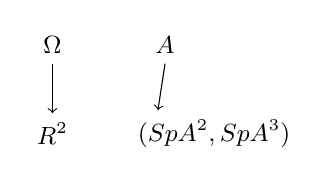
\begin{tikzpicture}[font=\small]
\node (o) at (-.86,.56) {$\Omega$};
\node (r) at (-.86,-.56) {$\mathbb R^2$};
\node (a) at (.57,.56) {$A$};
\node[anchor=west] (t) at (.1,-.56) {$(\operatorname{Sp}A^2,\operatorname{Sp}A^3)$};
\draw[->] (o)--(r);
\draw[->] (a.south)--([xshift=.38cm]t.north west);
\end{tikzpicture}}\endgroup
\end{center}
}
\end{GelfandAdjacentEvidence}
\begin{GelfandAdjacentEvidence}{GELFAND-P001079}{9}


Проекция $\Omega$ на $\mathbb R^2$ — это почти прав. 6-уг.

\SourceFigure{GELFAND-P001079}{hexagon-diagram}{%
\begin{center}
\begingroup\color{black}\GelfandFitDiagram{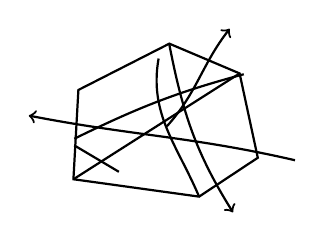
\begin{tikzpicture}[x=1.05cm,y=1.05cm,thick]
\coordinate (a) at (-1.11,-.67);
\coordinate (b) at (-1.05,.41);
\coordinate (c) at (.05,.97);
\coordinate (d) at (.9,.61);
\coordinate (e) at (1.12,-.41);
\coordinate (f) at (.41,-.88);
\draw (a)--(b)--(c)--(d)--(e)--(f)--cycle;
\draw (a)--(d);
\draw (-1.1,-.18) to[out=26,in=195] (.95,.6);
\draw (-1.1,-.26)--(-.56,-.58);
\draw (-.08,.79) to[out=-100,in=113] (.41,-.88);
\draw[->] (1.57,-.44) to[out=167,in=-11] (-1.65,.1);
\draw[->] (.02,-.03) to[out=48,in=232] (.78,1.15);
\draw[->] (.05,.96) to[out=-79,in=122] (.82,-1.07);
\end{tikzpicture}}\endgroup
\end{center}
В местах наложения штрихов отдельные соединения неясны.}
\end{GelfandAdjacentEvidence}
\begin{GelfandAdjacentEvidence}{GELFAND-P001079}{10}


(Все углы по $120^\circ$; стор. равны через $1$.)

Структ. слоя меняется. Особ. известны,\\
Многочлены — ?
\SourceFigure{GELFAND-P001079}{hexagon-final-caption}{Заключительная запись о строении слоя.}
\end{GelfandAdjacentEvidence}



\Needspace{7\baselineskip}
\begin{GelfandAdjacentEvidence}{GELFAND-P001080}{1}
\SourcePage{GELFAND-P001080}{6}
Из выпис. выше \uline{ф-л} \uline{вычисл.} кратности веса.
\SourceFigure{GELFAND-P001080}{weight-multiplicity-line}{Строка о кратностях веса с двумя подчёркиваниями.}
\end{GelfandAdjacentEvidence}



\Needspace{7\baselineskip}
\begin{GelfandAdjacentEvidence}{GELFAND-P001081}{1}
\SourcePage{GELFAND-P001081}{unlabelled}
\uuline{21/II-83 г.}\qquad\uline{Сем. Гельфанда}.

\uline{В. И. Арнольд.}
\SourceFigure{GELFAND-P001081}{arnold-heading}{Дата, название семинара и имя докладчика.}
\end{GelfandAdjacentEvidence}
\begin{GelfandAdjacentEvidence}{GELFAND-P001081}{2}


\begin{equation*}
(1)\qquad \ddot x+(\omega^2+\varepsilon a(t))x=0
\end{equation*}
\[
a(t+2\pi)=a(t)
\]

\SourceFigure{GELFAND-P001081}{instability-tongues}{%
\begin{center}
\begingroup\color{black}\GelfandFitDiagram{\begin{tikzpicture}[x=.97cm,y=.94cm,font=\small]
\draw (-.21,0)--(3.94,0);
\draw (0,-.23)--(0,1.38);
\node at (-.69,.67) {(2)};
\node[left] at (0,1.43) {$\varepsilon$};
\node[right] at (3.96,-.13) {$\omega$};
\draw (.17,.99) .. controls (.31,.73) and (.43,.51) .. (.54,0)
 .. controls (.68,.31) and (.93,.76) .. (1.12,.92);
\draw (.49,.24)--(.62,.29) (.45,.37)--(.69,.47)
 (.4,.51)--(.65,.61) (.39,.64)--(.71,.76)
 (.42,.76)--(.72,.85) (.39,.89)--(.72,.96);
\draw (1.17,.88) .. controls (1.22,.61) and (1.2,.33) .. (1.19,0)
 .. controls (1.33,.28) and (1.4,.71) .. (1.56,.9);
\draw (1.21,.28)--(1.31,.32) (1.22,.38)--(1.35,.41)
 (1.23,.49)--(1.35,.54) (1.26,.58)--(1.37,.62)
 (1.25,.68)--(1.37,.72) (1.26,.8)--(1.39,.82);
\draw (1.89,.99) .. controls (1.87,.63) and (1.86,.27) .. (1.85,0)
 .. controls (1.98,.29) and (2.07,.72) .. (2.17,1.03);
\draw (1.87,.23)--(1.94,.26) (1.87,.35)--(1.99,.39)
 (1.87,.47)--(2.04,.52) (1.93,.68)--(2.05,.73)
 (1.95,.83)--(2.06,.87) (1.96,.9)--(2.1,.94);
\draw (2.46,1.01) .. controls (2.48,.68) and (2.45,.31) .. (2.44,0)
 .. controls (2.54,.26) and (2.62,.66) .. (2.66,1.03);
\draw (2.47,.35)--(2.55,.36) (2.47,.48)--(2.58,.52)
 (2.47,.58)--(2.61,.63) (2.47,.69)--(2.63,.74)
 (2.47,.82)--(2.64,.82);
\draw[->] (3.02,1.2) .. controls (2.98,1.43) and (2.65,1.15) .. (2.49,.89);
\draw (1.19,0)--(1.19,-.08) (1.85,0)--(1.85,-.08) (2.44,0)--(2.44,-.08);
\node[below] at (.54,-.06) {$\frac12$};
\node[below] at (1.19,-.06) {$1$};
\node[below] at (1.85,-.06) {$\frac32$};
\node[below] at (2.44,-.06) {$2$};
\node[align=left,anchor=west] at (4.34,.55) {области\\неустойчивости};
\end{tikzpicture}}\endgroup
\end{center}
}
\end{GelfandAdjacentEvidence}
\begin{GelfandAdjacentEvidence}{GELFAND-P001081}{3}


$a(t)=\cos t\quad\Rightarrow$ касание всё более высокого порядка (границ зон).
\SourceFigure{GELFAND-P001081}{mathieu-tongue}{%
\begin{center}
\begingroup\color{black}\GelfandFitDiagram{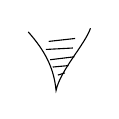
\begin{tikzpicture}[x=.93cm,y=.93cm]
\draw (-.38,.8) .. controls (-.16,.55) and (-.03,.32) .. (0,0)
 .. controls (.06,.28) and (.39,.62) .. (.47,.85);
\draw (.025,.21)--(.12,.24) (-.045,.32)--(.17,.34)
 (-.08,.42)--(.25,.46) (-.14,.56)--(.23,.58) (-.1,.67)--(.26,.71);
\end{tikzpicture}}\endgroup
\end{center}
Рисунок над словами «границ зон».}
\end{GelfandAdjacentEvidence}
\begin{GelfandAdjacentEvidence}{GELFAND-P001081}{4}


(3) \uline{Теор.} Ширина $N$-й зоны $\asymp\varepsilon^{[\frac Np]}$;
если $a$ — триг. многочлен
\[
\deg a=p.
\]
\Unclear{GELFAND-P001081}{zone-width-exponent}{В показателе степени написано $[N/p]$. Смысл скобок не оговорён.}
\end{GelfandAdjacentEvidence}
\begin{GelfandAdjacentEvidence}{GELFAND-P001081}{5}


\dashuline{Мате}: $p=1$.
\Unclear{GELFAND-P001081}{mathieu-name}{Написание имени читается как «Мате».}
\end{GelfandAdjacentEvidence}
\begin{GelfandAdjacentEvidence}{GELFAND-P001081}{6}


Ур-е Хилла ($a$ общего положения) $\Rightarrow$ всюду касание $1$-го пор.
\SourceFigure{GELFAND-P001081}{hill-tongue}{%
\begin{center}
\begingroup\color{black}\GelfandFitDiagram{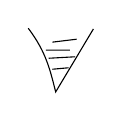
\begin{tikzpicture}[x=.93cm,y=.93cm]
\draw (-.42,.87) .. controls (-.17,.54) and (-.12,.29) .. (-.045,0)--(.47,.86);
\draw (-.09,.31)--(.13,.33) (-.14,.46)--(.22,.48)
 (-.18,.57)--(.15,.57) (-.09,.68)--(.24,.72);
\end{tikzpicture}}\endgroup
\end{center}
Рисунок после стрелки.}
\end{GelfandAdjacentEvidence}
\begin{GelfandAdjacentEvidence}{GELFAND-P001081}{7}


(но ширина $\exp$ убывает)

\dashuline{Вопр. И.М.Г.}: \dashuline{$\omega^2$ — $0$-зонный потенциал}.
Что будет вблизи $1$-зонного потенциала?
\SourceFigure{GELFAND-P001081}{gelfand-question}{Вопрос о потенциале с одной зоной.}
\end{GelfandAdjacentEvidence}
\begin{GelfandAdjacentEvidence}{GELFAND-P001081}{8}


\dashuline{Док-во} зав. от структуры ряда Рэлея-Шредингера. Ищем возмущ.
\begin{equation*}
(4)\quad
(\Lambda+\varepsilon A)(\xi_0+\varepsilon\xi_1+\ldots)
=(\xi_0+\varepsilon\xi_1+\ldots)(\lambda_0+\varepsilon\lambda_1+\ldots)
\end{equation*}
\SourceFigure{GELFAND-P001081}{perturbation-series}{Ряд возмущений в формуле (4).}
\end{GelfandAdjacentEvidence}



\Needspace{7\baselineskip}
\begin{GelfandAdjacentEvidence}{GELFAND-P001082}{1}
\SourcePage{GELFAND-P001082}{unlabelled}
ряды сверт. и зав. от чисел \uline{Каталана}:
\Unclear{GELFAND-P001082}{first-line-abbreviation}{Сокращение предположительно «сверт.».}
\end{GelfandAdjacentEvidence}
\begin{GelfandAdjacentEvidence}{GELFAND-P001082}{2}

\[
1\quad 1\quad 2\quad 5\quad 14\quad 42\quad 138
\]
\SourceFigure{GELFAND-P001082}{catalan-number}{Последнее число в рукописи — $138$.}
\end{GelfandAdjacentEvidence}
\begin{GelfandAdjacentEvidence}{GELFAND-P001082}{3}


Другое появл.: у Гриффитса и Харриса (они не заметили).

\uline{Ф-ла}:
\[
(5)\qquad a_{n+1}=\sum_{j=1}^{n-1}a_j a_{n-j}
\]
\SourceFigure{GELFAND-P001082}{catalan-recurrence}{Пределы суммы и индексы в рукописи.}
\end{GelfandAdjacentEvidence}
\begin{GelfandAdjacentEvidence}{GELFAND-P001082}{4}


Через произв. ф-ю считаем
\[
a_n=\frac{(2n)!}{n!(n+1)!}
\]
($=$ число симплиц. разбиений $n$-угольника)
\SourceFigure{GELFAND-P001082}{polygon-index}{Обозначение $n$-угольника в рукописи.}
\end{GelfandAdjacentEvidence}
\begin{GelfandAdjacentEvidence}{GELFAND-P001082}{5}


[Слева вверху вставлено «Гриффитс, Харрис»:]\\
Рим. пов. рода $g$ имеют $3g-3$ модуля.
\SourceFigure{GELFAND-P001082}{griffiths-harris-insertion}{Имена в приписке над строкой.}
\end{GelfandAdjacentEvidence}
\begin{GelfandAdjacentEvidence}{GELFAND-P001082}{6}


На $S^2=\mathbb C P^1$ выбир. точки ветвления и т.д.

ГХ: число способов, к-рыми получена одна [зачёркнуто] и та же пов.:
\Unclear{GELFAND-P001082}{genus-cancel}{Зачёркнутое слово, возможно, «пов.».}
\end{GelfandAdjacentEvidence}
\begin{GelfandAdjacentEvidence}{GELFAND-P001082}{7}

\[
1,1,2,5,\ldots\quad\text{— ч. Каталана (но не сказано — почему)}
\]

\dashuline{Скобочный символ}: выраже., правильно сост. из букв. и скобок:
пример
\[
((a))b\,(cd)e
\]
\[
\sum\text{числа символов и открыв. скобок}=n\quad\text{(длина)}
\]
\[
\Downarrow
\]
колич. $=$ числу Каталана

\SourceFigure{GELFAND-P001082}{bracket-symbol-examples}{%
\begin{center}
\begingroup\color{black}\GelfandFitDiagram{\begin{tikzpicture}[x=.87cm,y=.61cm,font=\small]
\node at (.45,0) {дл. 1};
\node at (1.69,0) {$a$};
\draw (-.13,-.38)--(2.18,-.38);
\draw (2.35,.25)--(2.35,-2.28)--(-.06,-2.28);
\node at (.45,-1.15) {дл. 2};
\node at (1.72,-.88) {$ab$};
\node at (1.72,-1.65) {$(a)$};
\draw (1.26,-.56)--(1.11,-.56)--(1.11,-2.12)--(1.28,-2.0);
\node at (3.73,-.12) {дл. 3};
\draw (3.27,-.48)--(4.53,-.48);
\draw (4.53,.31)--(4.53,-3.95)--(6.49,-3.95);
\draw (4.62,.43)--(6.65,.43) (6.58,.43)--(6.58,-3.83);
\node at (5.55,.0) {$a(b)$};
\node at (5.55,-.75) {$(a)b$};
\node at (5.55,-1.5) {$(ab)$};
\node at (5.55,-2.25) {$((a))$};
\node at (5.55,-3) {$abc$};
\end{tikzpicture}}\endgroup
\end{center}
}
\end{GelfandAdjacentEvidence}
\begin{GelfandAdjacentEvidence}{GELFAND-P001082}{8}


Скоб. символ $\rightsquigarrow$ член ряда теории возмущений.
\[
\underset{\text{соб. числа}}{\lambda_i}\quad\rightsquigarrow\quad\text{колчан}
\]

\uwave{Соб. числа.}\qquad $\Lambda$ — диаг. оператор,
\qquad $\Lambda_i:V_i\longrightarrow V_i$

\SourceFigure{GELFAND-P001082}{diagonal-operator-diagram}{%
\begin{center}
\begingroup\color{black}\GelfandFitDiagram{\begin{tikzpicture}[x=.85cm,y=.85cm,font=\small]
\node at (-.56,-.78) {(6)};
\draw (0,-2.15)--(0,.2)--(2.55,.2);
\draw (0,-.36)--(.56,-.36)--(.56,.2);
\node at (.28,-.07) {$\Lambda_i$};
\draw (.56,-.36) rectangle (1.06,-.86);
\draw[dotted,thick] (1.18,-.99)--(2.38,-2.14);
\end{tikzpicture}}\endgroup
\end{center}
\[
\underset{\text{матр. элем. возмущ.}}{A_{i,j}:V_i\longrightarrow V_j}
\]
}
\end{GelfandAdjacentEvidence}
\begin{GelfandAdjacentEvidence}{GELFAND-P001082}{9}


\SourceFigure{GELFAND-P001082}{quiver-diagram}{%
\begin{center}
\begingroup\color{black}\GelfandFitDiagram{\begin{tikzpicture}[x=.97cm,y=.94cm,font=\small]
\node[anchor=west] at (-.65,.72) {Колчан.};
\coordinate (i) at (0,0);
\coordinate (j) at (1.6,0);
\fill (i) circle (1.7pt) (j) circle (1.7pt);
\draw[->] (i) .. controls (.4,.18) and (.84,.22) .. (1.08,.13);
\draw (1.08,.13) .. controls (1.3,.1) and (1.49,.04) .. (j);
\draw[->] (1.49,-.12) .. controls (1.24,-.26) and (.81,-.3) .. (.52,-.23);
\draw (.52,-.23) .. controls (.33,-.15) and (.14,-.14) .. (.07,-.14);
\draw[->] (-.04,.23) .. controls (-.24,.81) and (-.81,.43) .. (-.79,-.06)
 .. controls (-.76,-.54) and (-.37,-.35) .. (-.17,-.23);
\node at (-.02,-.45) {$i$};
\node at (1.55,-.54) {$j$};
\node at (3.08,.46) {\uwave{стрелке $\rightsquigarrow A_{i,j}$}};
\node at (-.02,-1.05) {$V_i$};
\node at (1.55,-1.15) {$V_j$};
\node[align=left,anchor=west] at (1.9,-1.08) {— соб. подпр-ва\\(вершины)};
\end{tikzpicture}}\endgroup
\end{center}
}
\end{GelfandAdjacentEvidence}



\Needspace{7\baselineskip}
\begin{GelfandAdjacentEvidence}{GELFAND-P001083}{1}
\SourcePage{GELFAND-P001083}{9}
Пусть всё конечно или лок. конечно

(в $\forall$ вершину ведёт конечное число)

Ур-е Мате — колчан не полный!
\Unclear{GELFAND-P001083}{mathieu-name-top}{Написание имени читается как «Мате».}
\end{GelfandAdjacentEvidence}
\begin{GelfandAdjacentEvidence}{GELFAND-P001083}{2}


(лок. конечный)

(потенц. — $\cos$ и $\sin$ и соб. ф-и тоже!)

\uline{Мате} (с триг. многочл.) $\Rightarrow$ матр. типа обобщ. Якобиевой.
\Unclear{GELFAND-P001083}{mathieu-name-lower}{Написание имени читается как «Мате».}
\end{GelfandAdjacentEvidence}
\begin{GelfandAdjacentEvidence}{GELFAND-P001083}{3}


Ищем возмущение $\lambda_0$.

\SourceFigure{GELFAND-P001083}{spectral-graph-diagram}{%
\begin{center}
\begingroup\color{black}\GelfandFitDiagram{\begin{tikzpicture}[x=1.04cm,y=1.04cm]
\draw (-.47,0)--(2.1,0);
\draw (0,0)--(0,1.41);
\draw (-.48,-.17)--(2.18,.45);
\node[left] at (0,1.33) {$\displaystyle\bigoplus_{i\ne0}V_i$};
\node[below] at (2.16,0) {$V_0$};
\node[below] at (.9,-.06) {$\lambda_0$};
\node[right] at (2.18,.45) {$V_0(\varepsilon)$};
\end{tikzpicture}}\endgroup
\end{center}
}
\end{GelfandAdjacentEvidence}
\begin{GelfandAdjacentEvidence}{GELFAND-P001083}{4}


$V_0(\varepsilon)$ — подпр-во, [ниже: «собств.»] аналит. завис. от
$\varepsilon$, соотв. соб. вект., близким к $\lambda_0$.
\SourceFigure{GELFAND-P001083}{eigenvalue-word}{Сокращение «соб. вект.» в рукописи.}
\end{GelfandAdjacentEvidence}
\begin{GelfandAdjacentEvidence}{GELFAND-P001083}{5}


\[
(7)\quad
(\Lambda+\varepsilon A)(E_0+B(\varepsilon))
=(E_0+B(\varepsilon))(\lambda_0+\varepsilon\alpha^1+\ldots)
\]
\SourceFigure{GELFAND-P001083}{coefficient-symbol}{Коэффициент $\alpha^1$ в формуле (7).}
\end{GelfandAdjacentEvidence}
\begin{GelfandAdjacentEvidence}{GELFAND-P001083}{6}


$V_0(\varepsilon)$ — график оператора
\[
B(\varepsilon):V_0\longrightarrow\bigoplus_{i\ne0}V_i
\qquad E_0\text{ — проектор на }V_0
\]
\[
\alpha^1:\text{ оператор }V_0\to V_0,\qquad \alpha^i:V_0\to V_0
\]

(7) — условие инвариантности [зачёркнуто] $V_0(\varepsilon)$
\Unclear{GELFAND-P001083}{invariance-cancel}{Зачёркнутый знак неразборчив.}
\end{GelfandAdjacentEvidence}
\begin{GelfandAdjacentEvidence}{GELFAND-P001083}{7}


(8) опер. $\lambda_0+\varepsilon\alpha^1+\ldots$ наз.
\uwave{секулярным} опер. (в физике)
\Unclear{GELFAND-P001083}{secular-ending}{Над окончанием слова «секулярным» видна поправка. Первоначальное окончание неясно.}
\end{GelfandAdjacentEvidence}
\begin{GelfandAdjacentEvidence}{GELFAND-P001083}{8}


Сужение $\Lambda+\varepsilon A$ на $V_0(\varepsilon)$
подобно секул. опер. (8) $\Rightarrow$ у них одинак. соб. числа.

\uwave{Ф-ла для $\alpha^k$}:
\[
(9)\qquad \alpha_k=\sum_{\gamma:\lvert\gamma\rvert=k}
\bigl(\Pi_\gamma(A)Q_\gamma(\Lambda)\bigr)
\]
\SourceFigure{GELFAND-P001083}{loop-coefficient-formula}{В заголовке индекс сверху, а в формуле (9) — снизу.}
\end{GelfandAdjacentEvidence}
\begin{GelfandAdjacentEvidence}{GELFAND-P001083}{9}


$\gamma$ — петля в колчане из $0$ в $0$

$k$ — длина петли

\SourceFigure{GELFAND-P001083}{loop-diagram}{%
\begin{center}
\begingroup\color{black}\GelfandFitDiagram{\begin{tikzpicture}[x=1.06cm,y=1.06cm]
\coordinate (origin) at (0,1.46);
\coordinate (first) at (1.96,1.66);
\coordinate (left) at (.34,-.07);
\coordinate (right) at (1.25,-.02);
\coordinate (m) at (-1.39,.02);
\node at (-1.78,.99) {(10)};
\node[above left] at (origin) {$0$};
\node[right] at (first) {$i$};
\node[below left] at (m) {$m$};
\node[below right] at (left) {$j$};
\node[right] at (right) {$j$};
\node at (1.03,.99) {$\gamma$};
\draw[->] (m)--(-.43,1.02);
\draw (-.43,1.02)--([xshift=-.07cm,yshift=-.06cm]origin);
\draw[->] ([xshift=.11cm]origin)--(1.25,1.58);
\draw (1.25,1.58)--(first);
\draw[->] (first)--(1.62,.82);
\draw (1.62,.82)--(right);
\draw[->] ([xshift=-.15cm]right)--(.26,1.12);
\draw (.26,1.12)--(origin);
\draw[->] (origin)--(.26,.44);
\draw (.26,.44)--(left);
\draw[->] ([xshift=-.03cm]left)--(-.97,.015);
\draw (-.97,.015)--(m);
\draw[<->] (.73,-.26)--(1.22,-.19);
\draw[->] (.61,-.17)--(.36,.06);
\end{tikzpicture}}\endgroup
\end{center}
Обе нижние подписи похожи на $j$. Соединение короткого косого штриха с соседними стрелками неясно.}
\end{GelfandAdjacentEvidence}
\begin{GelfandAdjacentEvidence}{GELFAND-P001083}{10}


\[
\Pi_\gamma(A)=A_{m0}\ldots A_{ij}A_{0i}
\]

$\Pi_\gamma(A)$ — хронологическое произведение петли
($=\prod A_{i,j}$ в нужном порядке по петле)
[ниже приписано: «по стрелкам».]
\SourceFigure{GELFAND-P001083}{chronological-insertion}{Приписка под пояснением порядка множителей.}
\end{GelfandAdjacentEvidence}


$Q_\gamma(\Lambda)$ — рац. ф-я от соб. чисел

(вычис. через числа Каталана!)

Рассм. скоб. символ.

\uwave{Заполнение его} — вставл. вершин колчана вместо букв.


\Needspace{7\baselineskip}
\begin{GelfandAdjacentEvidence}{GELFAND-P001084}{1}
\SourcePage{GELFAND-P001084}{unlabelled}
По заполнению строится петля.

\Unclear{GELFAND-P001084}{top-cancel}{Зачёркнутый знак перед словом «Слагаемые» неразборчив.}
\end{GelfandAdjacentEvidence}
\begin{GelfandAdjacentEvidence}{GELFAND-P001084}{2}

Слагаемые надо нумеровать заполнениями

\[
\Vert\quad 0\longrightarrow 0\longrightarrow i\longrightarrow j\longrightarrow 0
\]
\SourceFigure{GELFAND-P001084}{first-loop}{Цепочка из четырёх стрелок с двумя начальными нулями.}
\end{GelfandAdjacentEvidence}
\begin{GelfandAdjacentEvidence}{GELFAND-P001084}{3}


\[
\begin{array}{cl}
(i)j & \\
\downarrow & \\
0 & \text{по открытой скобке, закрытые опускаем}
\end{array}
\]
\SourceFigure{GELFAND-P001084}{bracket-rule}{Стрелка от открытой скобки к нулю и пояснение.}
\end{GelfandAdjacentEvidence}
\begin{GelfandAdjacentEvidence}{GELFAND-P001084}{4}


Стрелок на 1 больше, чем длина заполнения.

1 петля — из разных заполнений.

\[
0\longrightarrow i\longrightarrow j\longrightarrow 0
\longrightarrow j\longrightarrow m\longrightarrow 0
\]
\SourceFigure{GELFAND-P001084}{second-loop}{Петля с двумя вхождениями вершины $j$.}
\end{GelfandAdjacentEvidence}
\begin{GelfandAdjacentEvidence}{GELFAND-P001084}{5}


Сумма на самом деле не по петлям, а заполнениям.

[Зачёркнута строка: $ij(jm)\quad ij(jm)$ не од…]
\Unclear{GELFAND-P001084}{cancelled-fillings}{В зачёркнутой строке читаются два похожих заполнения. Справа, возможно, «не од…».}
\end{GelfandAdjacentEvidence}
\begin{GelfandAdjacentEvidence}{GELFAND-P001084}{6}


$ij(jm\qquad$ не однозн. закрыв. скобка!! —
\SourceFigure{GELFAND-P001084}{closing-bracket-ambiguity}{Запись без закрывающей скобки и замечание к ней.}
\end{GelfandAdjacentEvidence}
\begin{GelfandAdjacentEvidence}{GELFAND-P001084}{7}


\tikz[baseline=(repeat.base)]{\node[draw,rounded corners=3pt,inner sep=2pt] (repeat) {повтор.};}\quad [зачёркнуто] вклад [зачёркнуто]
\Unclear{GELFAND-P001084}{cancelled-before-exit}{Под обведённым словом, вероятно, зачёркнуто «— тот же».}
\end{GelfandAdjacentEvidence}
\begin{GelfandAdjacentEvidence}{GELFAND-P001084}{8}

\Unclear{GELFAND-P001084}{cancelled-after-exit}{После «вклад», вероятно, зачёркнуто «разные скобки!!».}
\end{GelfandAdjacentEvidence}
\begin{GelfandAdjacentEvidence}{GELFAND-P001084}{9}


Диаграмма заполнения: добавл. пунктирные [\sout{скобки}] [вписано ниже: стрелки]
\Unclear{GELFAND-P001084}{overwritten-adjective-ending}{Окончание в слове «пунктирные» переписано. Прежнее окончание неясно.}
\end{GelfandAdjacentEvidence}
\begin{GelfandAdjacentEvidence}{GELFAND-P001084}{10}


\SourceFigure{GELFAND-P001084}{filling-diagram}{%
\begin{center}
\begingroup\color{black}\GelfandFitDiagram{\begin{tikzpicture}[x=1cm,y=.86cm,font=\small]
\node at (-1.12,-.04) {$(i)j$};
\node (outerleft) at (0,0) {$0$};
\node (opening) at (1.04,.01) {$0$};
\node (inside) at (2.19,.05) {$i$};
\node (outside) at (3.27,.09) {$j$};
\node (outerright) at (4.5,.13) {$0$};
\draw[->] (outerleft)--(opening);
\draw[->] (opening)--(inside);
\draw[->] (inside)--(outside);
\draw[->] (outside)--(outerright);
\draw[->,dashed] (inside.north) to[bend right=53] (opening.north);
\draw (.1,-.39)--(.1,-.81)--(-.44,-.78);
\draw (4.44,-.22)--(4.44,-.48)--(5.13,-.48);
\end{tikzpicture}}\endgroup
\end{center}
}
\end{GelfandAdjacentEvidence}
\begin{GelfandAdjacentEvidence}{GELFAND-P001084}{11}

крайние нули ничего не значат

Стрелка $\longrightarrow$ в $0$, соотв. открыв. скобке, соответствующей
[зачёркнуто] закрыв. скобке (из буквы до закрыв. скобки)
\Unclear{GELFAND-P001084}{cancelled-open}{Вероятное чтение зачёркнутого слова «открыв.».}
\end{GelfandAdjacentEvidence}
\begin{GelfandAdjacentEvidence}{GELFAND-P001084}{12}


\begin{equation*}
\alpha_k=\sum_{I,\ \lvert I\rvert=k-1}\frac{\Pi_{\gamma(I)}(A)}{q_I(\Lambda)}
\tag{11}
\end{equation*}
\SourceFigure{GELFAND-P001084}{coefficient-formula}{В левой части формулы (11) записано $\alpha_k$.}
\end{GelfandAdjacentEvidence}
\begin{GelfandAdjacentEvidence}{GELFAND-P001084}{13}


\[
\begin{array}{l}
I\\[-.3ex]
\vert\\[-.3ex]
\text{заполнение скоб. символа}
\end{array}
\qquad
\lvert I\rvert\text{ — длина скоб. символа}
\]
\SourceFigure{GELFAND-P001084}{bracket-symbol-ending}{Две подписи к индексу суммирования.}
\end{GelfandAdjacentEvidence}
\begin{GelfandAdjacentEvidence}{GELFAND-P001084}{14}


$\Pi_{\gamma(I)}(A)$ — хрон. произв. петли по сплошным стрелкам.

\begin{equation*}
q_I(\Lambda)=
\underset{\substack{\text{сплошные}\\\text{стрелки}\\\text{в }i}}
{\prod_{i\ne0}}(\lambda_0-\lambda_i)
\underset{\substack{\text{пункт.}\\\text{стрелки}\\\text{из }j}}
{\prod_{j\ne0}}(\lambda_j-\lambda_0)
\tag{12}
\end{equation*}
\SourceFigure{GELFAND-P001084}{denominator-formula}{Множители и подписи к двум произведениям в формуле (12).}
\end{GelfandAdjacentEvidence}
\begin{GelfandAdjacentEvidence}{GELFAND-P001084}{15}


\[
(i)j\rightsquigarrow
(\lambda_0-\lambda_i)(\lambda_0-\lambda_j)(\lambda_i-\lambda_0)
\]
\SourceFigure{GELFAND-P001084}{denominator-example}{Произведение для заполнения $(i)j$.}
\end{GelfandAdjacentEvidence}



\Needspace{7\baselineskip}
\begin{GelfandAdjacentEvidence}{GELFAND-P001085}{1}
\SourcePage{GELFAND-P001085}{10}
Для четных триг. многочленов достат. ф-ии (9)

[Под словом «четных»: (по $\cos$)]

(и отдельно для $\sin$ тоже)
\SourceFigure{GELFAND-P001085}{cosine-insertion}{Приписка о косинусе под словом «четных».}
\end{GelfandAdjacentEvidence}
\begin{GelfandAdjacentEvidence}{GELFAND-P001085}{2}


\[
V=\bigoplus V_i
\]
\begin{equation*}
\Lambda=\frac{d^2}{dt^2},\qquad
V_k=\{e_k,e_{-k}\},\qquad e_k=e^{ikt}
\tag{13}
\end{equation*}
\SourceFigure{GELFAND-P001085}{fourier-basis}{Обозначения оператора и базиса в формуле (13).}
\end{GelfandAdjacentEvidence}
\begin{GelfandAdjacentEvidence}{GELFAND-P001085}{3}


\[
\begin{array}{c c c c c c c}
 & V_0, & V_1, & V_2 & V_3 & \cdots & V_k\\
\dim & 1 & 2 & 2 & 2 & & 2\\
 & & & & & & \lambda=-k^2
\end{array}
\]
\SourceFigure{GELFAND-P001085}{eigenspace-dimensions}{Размерности и собственное число в последнем столбце.}
\end{GelfandAdjacentEvidence}
\begin{GelfandAdjacentEvidence}{GELFAND-P001085}{4}


$A$ — умн. на триг. многочлен

\begin{equation*}
a(t)=\sum_{\lvert s\rvert\le p}a_se_s
\tag{14}
\end{equation*}

Пусть он чётный, т.е.
\begin{equation*}
a_{-s}=a_s
\tag{15}
\end{equation*}

\begin{equation*}
A_{i,j}=
\begin{pmatrix}
a_{j-i} & a_{i+j}\\
a_{-i-j} & a_{i-j}
\end{pmatrix}
\qquad (?)
\tag{16}
\end{equation*}
\SourceFigure{GELFAND-P001085}{matrix-display}{Знаки индексов и знак вопроса рядом с формулой (16).}
\end{GelfandAdjacentEvidence}
\begin{GelfandAdjacentEvidence}{GELFAND-P001085}{5}


$(16)\Rightarrow$ если $i+j>p$, то матрицы диагон. и даже \uline{скалярны}
[ниже: (ввиду (15))] в этом базисе.

Если все $A_{i,j}$ в петле скалярны, то и произвед. скалярно.

\begin{equation*}
\underline{\tau p<2k}\quad\Rightarrow\quad
\text{\uwave{$\alpha_\tau$ скалярно}}
\tag{17}
\end{equation*}
\SourceFigure{GELFAND-P001085}{scalar-lemma}{Коэффициент $\alpha_\tau$ и подчёркивания в формуле (17).}
\end{GelfandAdjacentEvidence}
\begin{GelfandAdjacentEvidence}{GELFAND-P001085}{6}


Это — топологич. лемма (из комбинат. топ.)

\uline{Д-во}

\SourceFigure{GELFAND-P001085}{proof-number-line}{%
\begin{center}
\begingroup\color{black}\GelfandFitDiagram{\begin{tikzpicture}[x=.59cm,y=.72cm,font=\small]
\draw (-.88,0)--(0,0)--(1.31,.06)--(3.38,.02)--(6.05,-.09)--(9.23,-.16);
\foreach \x/\y in {0/0,.62/.02,1.31/.06,1.96/.045,2.70/.034,3.38/.02,
  4.15/-.01,4.80/-.04,5.34/-.06,6.05/-.09,6.79/-.105,7.43/-.12,
  8.12/-.135,8.74/-.15}
  \draw (\x,\y-.13)--(\x,\y+.13);
\node at (0,-.44) {$-k$};
\node at (4.15,-.45) {$0$};
\node at (8.74,-.56) {$k$};
\end{tikzpicture}}\endgroup
\end{center}
}
\end{GelfandAdjacentEvidence}
\begin{GelfandAdjacentEvidence}{GELFAND-P001085}{7}


Рассм. петлю из $\tau$ стрелок длины $\le p$.

Тогда для $\forall$ стрелки $i+j>p$

(гомотопна $0$!)

$i+j\le p\ \Rightarrow$ перескок
\Unclear{GELFAND-P001085}{crossing-word}{Предположительное чтение «перескок».}
\end{GelfandAdjacentEvidence}
\begin{GelfandAdjacentEvidence}{GELFAND-P001085}{8}


\SourceFigure{GELFAND-P001085}{loop-arches}{%
\begin{center}
\begingroup\color{black}\GelfandFitDiagram{\begin{tikzpicture}[x=1.16cm,y=.83cm,font=\small]
\draw (-1.8,.16) .. controls (-1.32,.54) and (-.84,.87) .. (-.34,.49)
 .. controls (-.21,.41) and (-.11,.33) .. (-.11,.12)
 .. controls (-.01,.37) and (.33,.37) .. (.46,.11)
 .. controls (.59,.42) and (1.56,.98) .. (2.13,.23);
\node[below] at (-1.84,.07) {$-k$};
\node[below] at (2.18,.05) {$+k$};
\node at (2.24,.03) {$i$};
\end{tikzpicture}}\endgroup
\end{center}
Малый знак у правого конца похож на $i$. Наконечники на дугах неразличимы.}
\end{GelfandAdjacentEvidence}

$\Rightarrow$ длина $\le\tau p$ и т.д.

$(17)\Rightarrow$ в этом приближении соб. число ещё не расщепилось $\Rightarrow$

$\Rightarrow$ нужное нер-во!


\Needspace{7\baselineskip}
\begin{GelfandAdjacentEvidence}{GELFAND-P001086}{1}
\SourcePage{GELFAND-P001086}{unlabelled}
Ещё используется инволюция:
\[
(((a))b)(cd)e
\]
\SourceFigure{GELFAND-P001086}{original-bracket-symbol}{Исходный скобочный символ.}
\end{GelfandAdjacentEvidence}
\begin{GelfandAdjacentEvidence}{GELFAND-P001086}{2}


откр. скобками разбив. на фрагменты
\[
a))b)\qquad cd)e
\]
\SourceFigure{GELFAND-P001086}{first-fragments}{Фрагменты после удаления открывающих скобок.}
\end{GelfandAdjacentEvidence}
\begin{GelfandAdjacentEvidence}{GELFAND-P001086}{3}


Закрыв. скобки приклеиваем к букве. Переставл. буквы во фрагментах
[приписано ниже слева: в обр. порядке]
\SourceFigure{GELFAND-P001086}{reverse-order-insertion}{Приписка об обратном порядке букв.}
\end{GelfandAdjacentEvidence}
\begin{GelfandAdjacentEvidence}{GELFAND-P001086}{4}

\[
b)a))\qquad ed)c
\]
\SourceFigure{GELFAND-P001086}{reversed-fragments}{Два фрагмента с обратным порядком букв.}
\end{GelfandAdjacentEvidence}
\begin{GelfandAdjacentEvidence}{GELFAND-P001086}{5}


[зачёркнуто] Ставим откр. скобки на старые места
\Unclear{GELFAND-P001086}{cancel-before-stavim}{Зачёркнутое сокращение перед словом «Ставим» неразборчиво.}
\end{GelfandAdjacentEvidence}
\begin{GelfandAdjacentEvidence}{GELFAND-P001086}{6}

\[
(((b)a))(ed)c
\]
\SourceFigure{GELFAND-P001086}{dual-bracket-symbol}{Двойственный скобочный символ.}
\end{GelfandAdjacentEvidence}
\begin{GelfandAdjacentEvidence}{GELFAND-P001086}{7}


\uwave{Получ. двойств. символ}

Его вклад получается перестан. диаг. элементов.
\SourceFigure{GELFAND-P001086}{final-abbreviation}{В конце строки сокращено «диаг.».}
\end{GelfandAdjacentEvidence}



\Needspace{7\baselineskip}
\begin{GelfandAdjacentEvidence}{GELFAND-P001087}{1}
\SourcePage{GELFAND-P001087}{unlabelled}
\uline{28/II-83 г.}\qquad\uuline{Сем. Гельфанда}.

\uline{И. Кричевер.}
\SourceFigure{GELFAND-P001087}{krichever-heading}{Дата, название семинара и имя докладчика.}
\end{GelfandAdjacentEvidence}
\begin{GelfandAdjacentEvidence}{GELFAND-P001087}{2}


Цель — построить формальную теорию возмущ. для возмущения ур-я КдФ.
\begin{equation*}
(1)\qquad
u_t-\frac{\partial}{\partial x}
\underset{\frac{\delta I_3}{\delta u}}{%
\tikz[baseline=(term.base)]{
\node[inner sep=1pt] (term) {$\displaystyle\left(\frac14u_{xx}-\frac34u^2\right)$};
\draw (term.south west) -- ++(0,-.8mm) -| (term.south east);
}}
=\varepsilon K[u]
\end{equation*}
[Под $K$: дифф. полином от $u$.]
\SourceFigure{GELFAND-P001087}{perturbed-kdv-equation}{Формула (1) с прямоугольной скобкой и пометой под $K$.}
\end{GelfandAdjacentEvidence}
\begin{GelfandAdjacentEvidence}{GELFAND-P001087}{3}


[Зачёркнуто: \sout{\(u=u_0\)}.]
\SourceFigure{GELFAND-P001087}{cancelled-initial-condition}{Зачёркнутое равенство перед (2).}
\end{GelfandAdjacentEvidence}
\begin{GelfandAdjacentEvidence}{GELFAND-P001087}{4}

\[
(2)\qquad u=u_0(x,t)+\varepsilon(\ldots)
\]
КдФ
\begin{equation*}
(3)\qquad
u_t-\frac{\partial}{\partial x}
\underset{\substack{\Vert\\[.1ex]\frac{\delta I_3}{\delta u}}}{%
\tikz[baseline=(term.base)]{
\node[inner sep=1pt] (term) {$\displaystyle\left(\frac14u_{xx}-\frac34u^2\right)$};
\draw (term.south west) -- ++(0,-.8mm) -| (term.south east);
}}
=0,\qquad I_3=\frac14(u_x^2+u^3).
\end{equation*}
\Unclear{GELFAND-P001087}{eq03-variational-annotation}{Между нижней скобкой и её подписью стоят две короткие вертикальные черты. Их смысл неясен.}
\end{GelfandAdjacentEvidence}
\begin{GelfandAdjacentEvidence}{GELFAND-P001087}{5}


Имеется беск. серия инволют. интегралов $I_k$: $I_1=u$, $I_2=u^2$, $\ldots$
\SourceFigure{GELFAND-P001087}{integrals-line}{Значения первых интегралов, включая переписанное $u$ при $I_1$.}
\end{GelfandAdjacentEvidence}
\begin{GelfandAdjacentEvidence}{GELFAND-P001087}{6}


Конечнозонное реш. — реш. — стац. точка ф-ла
\[
(4)\qquad H=I_{n+2}-\sum_{k=1}^{n+1}c_k I_k
\]
т. е. решение ур-я
\[
(5)\qquad \frac{\delta H}{\delta u}=0
\]
\SourceFigure{GELFAND-P001087}{finite-gap-stationary}{Функционал и условие стационарности в формулах (4) и (5).}
\end{GelfandAdjacentEvidence}
\begin{GelfandAdjacentEvidence}{GELFAND-P001087}{7}


Рекурр. соотношение:
\[
(6)\qquad
\frac{d}{dx}\frac{\delta I_{n+1}}{\delta u}
=\left[\left(\frac{d}{dx}\right)^3+2u\frac{d}{dx}+u'\right]
\frac{\delta I_n}{\delta u}
\]
(с точн. до коэффициентов).
\SourceFigure{GELFAND-P001087}{recursion-relation}{Коэффициенты, штрих и индексы в формуле (6).}
\end{GelfandAdjacentEvidence}
\begin{GelfandAdjacentEvidence}{GELFAND-P001087}{8}


\[
\delta^2 H\; -\; ?
\]
в опр. стац. точке.
\SourceFigure{GELFAND-P001087}{second-variation}{Вопрос о второй вариации.}
\end{GelfandAdjacentEvidence}



\Needspace{7\baselineskip}
\begin{GelfandAdjacentEvidence}{GELFAND-P001088}{1}
\SourcePage{GELFAND-P001088}{15}
\[
L=-\frac{d^2}{dx^2}+u_0(x)\qquad
\text{спектр:}\qquad (u_0(x+1)=u_0(x))
\]
\SourceFigure{GELFAND-P001088}{periodic-schrodinger-operator}{Оператор и условие периодичности.}
\end{GelfandAdjacentEvidence}
\begin{GelfandAdjacentEvidence}{GELFAND-P001088}{2}


\SourceFigure{GELFAND-P001088}{spectrum-bands}{%
\begin{center}
\begingroup\color{black}\GelfandFitDiagram{\begin{tikzpicture}[x=.65cm,y=.64cm,font=\small]
\draw (0,0)--(.74,-.012) (1.39,.025)--(2.01,.003)
 (2.58,.003)--(3.36,.01) (3.76,.037)--(4.36,.063)
 (4.79,.026) to[out=5,in=177] (9.18,.095);
\foreach \x in {0,.74,1.39,2.01,2.58,3.36,3.76,4.36,4.79}
  \draw (\x,-.17)--(\x,.19);
\node[below] at (0,-.2) {$E_1$};
\node[below] at (.74,-.2) {$E_2$};
\node[below] at (1.39,-.2) {$E_3$};
\node[below] at (2.01,-.2) {$E_4$};
\node[below right] at (4.73,-.13) {$E_{2n+1}$};
\end{tikzpicture}}\endgroup
\end{center}
}
\end{GelfandAdjacentEvidence}
\begin{GelfandAdjacentEvidence}{GELFAND-P001088}{3}

Оставшиеся концы — простые соб. знач. периодич. и антипер. задач.

Дифференциал квазиимпульса:
\[
(7)\qquad
i\,dp=\frac{Q(E)dE}{\sqrt R}
=\frac{E^n+\sum_{k=1}^{n}r_kE^{n-k}}{\sqrt R}\,dE
\]
\Unclear{GELFAND-P001088}{eq07-polynomial-coefficient}{Коэффициент предположительно $r_k$. Начертание первой буквы неоднозначно.}
\end{GelfandAdjacentEvidence}
\begin{GelfandAdjacentEvidence}{GELFAND-P001088}{4}

\[
R(E)=\prod_{i=1}^{2n+1}(E-E_i)
\]
[Зачёркнуто справа: \sout{(норм.}]
\Unclear{GELFAND-P001088}{cancel-normalized}{Видно начало «(норм.». Дальнейшее сокращение неясно.}
\end{GelfandAdjacentEvidence}
\begin{GelfandAdjacentEvidence}{GELFAND-P001088}{5}


Условия, однозначно определяющие $dp$:
\[
\int_{E_{2i}}^{E_{2i+1}}dp=0
\]
(нормир. абелев дифференциал 2-го рода с единств. особ. на $\infty$ —\\
— полюс 2-го пор.)
\SourceFigure{GELFAND-P001088}{quasimomentum-normalization}{Нулевой интеграл и пояснение о полюсе.}
\end{GelfandAdjacentEvidence}
\begin{GelfandAdjacentEvidence}{GELFAND-P001088}{6}


Рассм. теперь возмущение $u=u_0+\delta u$

$E_i'$ — новые концы зон

$e_s^-<e_s^+$ — новые концы зон; $\delta e_s=e_s^+-e_s^-$
\SourceFigure{GELFAND-P001088}{new-endpoints}{Два новых конца и определение $\delta e_s$.}
\end{GelfandAdjacentEvidence}
\begin{GelfandAdjacentEvidence}{GELFAND-P001088}{7}


Тогда:
\[
(8)\qquad
\delta^2H=\frac12\sum Q(E_i)(\delta E_i)^2
+\frac14\sum_s Q(e_s)(\delta e_s)^2
\]
($e_s$ — 2-кратные точки спектра)
\SourceFigure{GELFAND-P001088}{second-variation-equation}{Две суммы второй вариации и подпись к $e_s$.}
\end{GelfandAdjacentEvidence}
\begin{GelfandAdjacentEvidence}{GELFAND-P001088}{8}


$Q$ меняет знак по 1 разу в $\forall$ из запрещ. зон $\Rightarrow$ по 1-му нулю в любой зоне
\SourceFigure{GELFAND-P001088}{zeros-of-q}{Слова «по 1-му нулю» в рукописи.}
\end{GelfandAdjacentEvidence}
\begin{GelfandAdjacentEvidence}{GELFAND-P001088}{9}


\SourceFigure{GELFAND-P001088}{q-sign-diagram}{%
\begin{center}
\begingroup\color{black}\GelfandFitDiagram{\begin{tikzpicture}[x=.63cm,y=.66cm,font=\small]
\node at (0,-.01) {$\ldots$};
\draw (1.37,0)--(1.93,0) (3.02,.03)--(3.76,.03);
\draw[->] (4.85,.035) to[out=2,in=176] (8.14,-.04);
\foreach \x in {1.37,1.93,3.02,3.76,4.85}
  \draw (\x,-.15)--(\x,.15);
\node at (1.67,.44) {$+$};
\node at (3.49,.52) {$-$};
\node at (6.04,.56) {$+$};
\node at (10.13,.17) {\uwave{знак $Q$}};
\draw[->] (3.15,-.97)--(3.29,-.27);
\end{tikzpicture}}\endgroup
\end{center}
}
\end{GelfandAdjacentEvidence}
\begin{GelfandAdjacentEvidence}{GELFAND-P001088}{10}

[Под стрелкой:] внутри [зачёркнуто] могут быть ещё слипшиеся $\Rightarrow$ доб. ещё полож. или отриц. квадрат
\Unclear{GELFAND-P001088}{cancel-before-mogut}{Зачёркнутое слово, возможно, «будут».}
\end{GelfandAdjacentEvidence}
\begin{GelfandAdjacentEvidence}{GELFAND-P001088}{11}

(из 2-й суммы в (8))
\SourceFigure{GELFAND-P001088}{sign-caption}{Помета под стрелкой диаграммы знаков.}
\end{GelfandAdjacentEvidence}
\begin{GelfandAdjacentEvidence}{GELFAND-P001088}{12}


\[
(9)\qquad L\Psi(x,E)=E\Psi
\]
\[
\Psi(x+1)=w\Psi,\qquad w=e^{iP},\qquad P=\int_{E_1}^{E}dp
\]
\SourceFigure{GELFAND-P001088}{bloch-equations}{Уравнение и множитель Блоха.}
\end{GelfandAdjacentEvidence}
\begin{GelfandAdjacentEvidence}{GELFAND-P001088}{13}


Ширина раскр. зоны
\[
(10)\qquad
(\delta e_s)^2=
\frac{\bigl|\langle(\delta u)\Psi^2\rangle\bigr|^2}{\langle|\Psi|^2\rangle}
\]
($\Psi$ — блох. ф-я, $\Psi(x,e_s)$)
\SourceFigure{GELFAND-P001088}{eq10-denominator}{В рукописи знаменатель $\langle\lvert \Psi\rvert^2\rangle$ без внешней степени.}
\end{GelfandAdjacentEvidence}
\begin{GelfandAdjacentEvidence}{GELFAND-P001088}{14}


$\langle\qquad\rangle$ — усредн. по периоду

$u_0=\mathrm{const}\Rightarrow$ получ. [зачёркнуто: \sout{средн.} …] коэфф. Фурье для возмущения.
\Incomplete{GELFAND-P001088}{cancel-before-fourier}{После «средн…» одно или несколько слов закрыты линиями зачёркивания.}
\end{GelfandAdjacentEvidence}
\begin{GelfandAdjacentEvidence}{GELFAND-P001088}{15}


\uline{Задача (ИМГ)}: посчитать 3-ю вариацию и т. п.
\SourceFigure{GELFAND-P001088}{gelfand-task}{Задача о третьей вариации.}
\end{GelfandAdjacentEvidence}



\Needspace{7\baselineskip}
\begin{GelfandAdjacentEvidence}{GELFAND-P001089}{1}
\SourcePage{GELFAND-P001089}{unlabelled}
Вернемся к (1); пусть $u$ — решение. Тогда в 1-м пор. по $\varepsilon$
\begin{equation*}
u(x,t)=u_0(x,t)+\varepsilon\sum_s
\bigl[a_s^+w_s^+(x,t)+a_s^-w_s^-(x,t)\bigr]
\tag{11}
\end{equation*}
\SourceFigure{GELFAND-P001089}{mode-expansion}{Знаки при двух слагаемых в формуле (11).}
\end{GelfandAdjacentEvidence}
\begin{GelfandAdjacentEvidence}{GELFAND-P001089}{2}


$w_s^\pm(x,t)$ — реш. линеариз. КдФ в окр. $n$-зонного решения.
Они наход. так: проращиваем зону в окр. $e_s$ и берем производную по длине нов. зоны.
[вставлено над строкой: «$(n+1)$-зон. потенц.».]
\SourceFigure{GELFAND-P001089}{finite-gap-insertion}{Приписка о $(n+1)$-зонном потенциале.}
\end{GelfandAdjacentEvidence}
\begin{GelfandAdjacentEvidence}{GELFAND-P001089}{3}

\begin{equation*}
w_s^\pm(x,t)=-2\frac{\partial^2}{\partial x^2}
\ln\theta\bigl(Ux+Vt+Z-A(e_s)\bigr)e^{2\pi isx+V_st}
\tag{12}
\end{equation*}
[В аргументе $\theta$ вписано $Vt+$ перед $Z$.]
\SourceFigure{GELFAND-P001089}{theta-formula}{Формула (12) с надстрочной вставкой.}
\end{GelfandAdjacentEvidence}
\begin{GelfandAdjacentEvidence}{GELFAND-P001089}{4}

\Unclear{GELFAND-P001089}{upper-formula-frequency}{В показателе экспоненты предположительно $V_st$. Первая буква может читаться иначе.}
\end{GelfandAdjacentEvidence}
\begin{GelfandAdjacentEvidence}{GELFAND-P001089}{5}


$\Psi^2_{s\pm}(x,t,E)$ — реш. ур-я, сопряж. к линеариз. ур-ю $KdV$.
\begin{equation*}
\left\langle\Psi^2_{s\pm}(x,t,E),w_s^\pm(x,t)\right\rangle=0,
\qquad s\ne s'
\tag{13}
\end{equation*}
(средн. по $x$)
\SourceFigure{GELFAND-P001089}{middle-orthogonality-indices}{Оба множителя имеют индекс $s$. Справа написано $s\ne s'$.}
\end{GelfandAdjacentEvidence}
\begin{GelfandAdjacentEvidence}{GELFAND-P001089}{6}


($\Rightarrow$ имеется разл. по базису)
\[
w_s^\pm,\quad \frac{\partial u}{\partial E_i},\quad
\frac{\partial u}{\partial\gamma_i}
\]
\Unclear{GELFAND-P001089}{middle-parameter-derivative}{Предположительно $\partial\gamma_i$ в последнем знаменателе. Первая буква параметра не вполне ясна.}
\end{GelfandAdjacentEvidence}
\begin{GelfandAdjacentEvidence}{GELFAND-P001089}{7}


\medskip
\uuline{Водзицки (Мариус).}
\SourceFigure{GELFAND-P001089}{wodzicki-heading}{Имя докладчика в рукописи.}
\end{GelfandAdjacentEvidence}
\begin{GelfandAdjacentEvidence}{GELFAND-P001089}{8}

\begin{equation*}
L_w=-\frac{d^2}{dx^2}+u(x)-w,\qquad x\in[0,T]
\tag{1}
\end{equation*}
(\uline{опер. Хилла}; $u$ — $T$-периодич.)

$\zeta$-ф-я:
\begin{equation*}
\zeta_{L_w}(s)=\sum_{\substack{\lambda\in\operatorname{Spec}L\\\lambda\ne w}}
(\lambda-w)^{-s},\qquad \operatorname{Re}s>\tfrac12.
\tag{2}
\end{equation*}
\SourceFigure{GELFAND-P001089}{zeta-definition}{Определение дзета-функции с областью сходимости.}
\end{GelfandAdjacentEvidence}
\begin{GelfandAdjacentEvidence}{GELFAND-P001089}{9}


Интересуемся: значениями в т. $s=1,2,3,\ldots$

Пусть
\begin{equation*}
\begin{gathered}
u(x)\text{ — конечнозонный},\\
w\in\{\alpha_0,\ldots,\alpha_{2n}\}\text{ — концы зон}
\end{gathered}
\tag{3}
\end{equation*}

\uline{И.М.Г.}\quad\dashuline{Костя:}

\uline{Доп}: \uwave{Hurwitz} 1899 [переписано]
$\displaystyle\sum\frac{1}{(n+a)^s}$
\Unclear{GELFAND-P001089}{lower-speaker-abbreviation}{Подчёркнутое сокращение предварительно читается «Доп:».}
\end{GelfandAdjacentEvidence}
\begin{GelfandAdjacentEvidence}{GELFAND-P001089}{10}

\Unclear{GELFAND-P001089}{lower-hurwitz-overwritten-word}{Короткая помета после «Hurwitz 1899» густо переписана.}
\end{GelfandAdjacentEvidence}
\begin{GelfandAdjacentEvidence}{GELFAND-P001089}{11}


\SourceFigure{GELFAND-P001089}{epstein-callout}{%
\begin{center}
\begingroup\color{black}\GelfandFitDiagram{\begin{tikzpicture}[font=\small]
\node[anchor=west] (series) at (0,.55) {$\displaystyle\sum_n\frac{1}{(n^2+a)^s}$};
\node[align=left,anchor=west] (cont) at ([xshift=2mm]series.east) {— прод. с беск. числом полюсов};
\draw (series.north west) to[out=-105,in=156] ([xshift=-4mm,yshift=-5mm]cont.south west);
\draw ([xshift=2mm,yshift=-.4mm]cont.south west)--++(4mm,-3mm);
\node[anchor=west] at ([xshift=6mm,yshift=-4.5mm]cont.south west) {$\zeta$-ф-я Эпштейна};
\end{tikzpicture}}\endgroup
\end{center}
}
\end{GelfandAdjacentEvidence}
\begin{GelfandAdjacentEvidence}{GELFAND-P001089}{12}

однор. полином: \dashuline{есть функц. ур-е.}
\[
\begin{aligned}
\frac{1}{(n^2+a)^s}
&=\frac{1}{\bigl(n^2(1+\frac{a}{n^2})\bigr)^s}
=\left(\frac1{n^2}-\frac a{n^4}+\frac{a^2}{n^6}+\cdots\right)^s\\
&=\frac{1}{n^{2s}}\left(-\frac{as}{n^{2s+2}}+\cdots\right)
\end{aligned}
\]
\SourceFigure{GELFAND-P001089}{lower-series-final-equality}{Последнее равенство в рукописи. Перед минусом отдельной единицы не видно.}
\end{GelfandAdjacentEvidence}
\begin{GelfandAdjacentEvidence}{GELFAND-P001089}{13}


\uwave{Вопрос ИМГ.}: какая арифметика, когда $a$ — рац. число.
\SourceFigure{GELFAND-P001089}{arithmetic-question}{Вопрос об арифметике при рациональном параметре.}
\end{GelfandAdjacentEvidence}



\Needspace{7\baselineskip}
\begin{GelfandAdjacentEvidence}{GELFAND-P001090}{1}
\SourcePage{GELFAND-P001090}{16}
\uline{М.В.}
\begin{equation*}
\begin{aligned}
T\frac{\displaystyle\prod_{i=1}^{n}(z-\alpha_i')}
{\sqrt{4(z-\alpha_0)\cdots(z-\alpha_{2n})}}\,dz
&\equiv T\varphi_\alpha(z)\frac{dz}{2\sqrt{z-\alpha}},\\
&\hspace{2em}\alpha\in\{\alpha_0,\ldots,\alpha_{2n}\}
\end{aligned}
\tag{4}
\end{equation*}
(опр. $\varphi_\alpha$)
\SourceFigure{GELFAND-P001090}{quasimomentum-identity}{Левая часть (4) с произведением в числителе.}
\end{GelfandAdjacentEvidence}
\begin{GelfandAdjacentEvidence}{GELFAND-P001090}{2}

\SourceFigure{GELFAND-P001090}{quasimomentum-right-hand}{Правая часть (4) и выбор $\alpha$.}
\end{GelfandAdjacentEvidence}
\begin{GelfandAdjacentEvidence}{GELFAND-P001090}{3}


(то же, что выше у Кричевера)\\
— дифф. квазиимп.,
\SourceFigure{GELFAND-P001090}{quasimomentum-abbreviation}{Сокращённое название дифференциала.}
\end{GelfandAdjacentEvidence}
\begin{GelfandAdjacentEvidence}{GELFAND-P001090}{4}


\SourceFigure{GELFAND-P001090}{upper-monodromy-graph}{%
\begin{center}
\begingroup\color{black}\GelfandFitDiagram{\begin{tikzpicture}[x=.58cm,y=.68cm,font=\scriptsize]
\draw[->] (0,0)--(8.64,0);
\fill (0,0) circle (.8pt);
\draw (.06,1.08)--(.49,1.08) (.79,1.07)--(2.14,1.07)
 (2.91,1.04)--(4.42,1.04) (4.64,1.04)--(5.81,1.04)
 (6.61,1.11)--(8.43,1.11);
\draw (-.12,-1.04)--(.43,-1.04) (.88,-1.03)--(2.01,-1.03)
 (2.91,-1.06)--(3.81,-1.06) (4.87,-1.01)--(8.98,-1.01);
\draw[very thick] (.88,-1.03)--(2.01,-1.03)
 (3.38,1.04)--(4.32,1.04) (5.12,-1.01)--(5.75,-1.01)
 (7.91,-1.04)--(8.98,-1.04);
\draw[dashed] (0,0)--(.06,1.08) (.88,0)--(.88,-1.03)
 (1.32,0)--(1.32,-1.58) (2.01,0)--(2.01,-1.03)
 (3.86,0)--(3.86,1.41) (5.5,0)--(5.5,-1.31);
\draw[thick] (-.02,1.6) .. controls (.20,.63) and (.54,-.45) .. (.88,-1.03)
 .. controls (1.08,-1.39) and (1.21,-1.58) .. (1.32,-1.58)
 .. controls (1.57,-1.58) and (1.86,-1.24) .. (2.01,-1.03)
 .. controls (2.75,-.18) and (3.23,1.41) .. (3.86,1.41)
 .. controls (4.52,1.41) and (4.9,-1.31) .. (5.5,-1.31)
 .. controls (6.02,-1.27) and (6.92,.23) .. (7.17,.71)
 .. controls (7.44,1.23) and (7.43,1.11) .. (7.64,1.11)
 .. controls (8.11,1.11) and (8.20,.18) .. (8.24,-.18)
 .. controls (8.29,-1.1) and (8.53,-1.16) .. (8.76,-.72);
\node[below] at (-.04,-.12) {$\alpha_0$};
\node[above] at (.93,.05) {$\alpha_1$};
\node[above] at (1.47,.08) {$\alpha_1'$};
\node[above] at (2.01,.05) {$\alpha_2$};
\node[below] at (3.87,-.11) {$\alpha_2'$};
\node[above] at (5.52,.05) {$\alpha_3'$};
\node[right] at (8.65,-.11) {$v$};
\node[align=center,anchor=north] at (4.48,-1.74)
  {След матрицы монодромии. $\operatorname{tr}\widehat T(w)$};
\end{tikzpicture}}\endgroup
\end{center}
Подпись у стрелки оси похожа на $v$ или $\nu$.}
\end{GelfandAdjacentEvidence}
\begin{GelfandAdjacentEvidence}{GELFAND-P001090}{5}

\uwave{$\alpha_j'$ — точки $\min$ и $\max$} $\operatorname{tr}\widehat T(w)$.
\SourceFigure{GELFAND-P001090}{critical-points-caption}{Подпись о точках минимума и максимума.}
\end{GelfandAdjacentEvidence}
\begin{GelfandAdjacentEvidence}{GELFAND-P001090}{6}


Введ. Универ. набор полиномов:
\begin{equation*}
F(u)=1+\sum_{i=1}^{\infty}c_i\frac{u^i}{i!}
\tag{5}
\end{equation*}
и тогда
\begin{equation*}
\left[u\frac{d}{du}+p\right][F(u)]^p
=p\cdot\sum_{k=0}^{\infty}Q_{p,k}(c_1,\ldots,c_k)\frac{u^k}{k!},
\qquad Q_{p,0}\equiv1.
\tag{6}
\end{equation*}
(определение $Q_{p,k}$)
\SourceFigure{GELFAND-P001090}{polynomial-definition}{Определяющее соотношение (6).}
\end{GelfandAdjacentEvidence}
\begin{GelfandAdjacentEvidence}{GELFAND-P001090}{7}


\begin{equation*}
\begin{aligned}
\widehat Q_{p,k}
&\equiv\frac{p+2k}{p+k}Q_{p,k}(c_1,\ldots,c_k)\\
&=\frac{p+2k}{p}\,k!
\sum_{\substack{\lvert\beta\rvert\le\min(k,p)\\\sum_{i=1}^k i\beta_i=k}}
\binom{p}{\lvert\beta\rvert}
\frac{\lvert\beta\rvert!}{(1!)^{\beta_1}\beta_1!\cdots(k!)^{\Lambda_k}\beta_k!}\\
&\qquad{}\times c_1^{\beta_1}\cdots c_k^{\beta_k}
\end{aligned}
\tag{7}
\end{equation*}
\Unclear{GELFAND-P001090}{middle-factorial-exponent}{Последний показатель в знаменателе похож на $\Lambda_k$.}
\end{GelfandAdjacentEvidence}
\begin{GelfandAdjacentEvidence}{GELFAND-P001090}{8}

\SourceFigure{GELFAND-P001090}{weighted-summation-conditions}{Условия суммирования под знаком суммы.}
\end{GelfandAdjacentEvidence}
\begin{GelfandAdjacentEvidence}{GELFAND-P001090}{9}

\SourceFigure{GELFAND-P001090}{weighted-monomials}{Множители с $c_1$ и $c_k$.}
\end{GelfandAdjacentEvidence}
\begin{GelfandAdjacentEvidence}{GELFAND-P001090}{10}

\[
\sum[F(u)]^p z^p=\frac{1}{1-zF(u)}=\Phi(u,z)
\]
и надо взять:
\[
\left(u\frac{\partial}{\partial u}+z\frac{\partial}{\partial z}\right)\Phi(u,z).
\]
\begin{equation*}
\log F(u)\equiv\sum Q_{0,k}(c_1,\ldots,c_k)\frac{u^k}{k}
\tag{8}
\end{equation*}
\Unclear{GELFAND-P001090}{lower-logarithm-denominator}{Знаменатель переписан. Читается $k$. Прежние штрихи неясны.}
\end{GelfandAdjacentEvidence}
\begin{GelfandAdjacentEvidence}{GELFAND-P001090}{11}

(опр. $Q_{0,k}$)

Построим:
\begin{equation*}
\xi_{-1}:=\varphi_\alpha^2(w)\big|_{w=\alpha},
\tag{9}
\end{equation*}
\begin{equation*}
\xi_i:=\frac{1}{2i+1}
\left.\frac{\varphi_\alpha^{(i)}(w)}{\varphi_\alpha(w)}\right|_{w=\alpha},
\qquad i=1,2,\ldots
\tag{10}
\end{equation*}
\SourceFigure{GELFAND-P001090}{endpoint-coefficients}{Подстановки и множитель $(2i+1)^{-1}$ в формулах (9) и (10).}
\end{GelfandAdjacentEvidence}



\Needspace{7\baselineskip}
\begin{GelfandAdjacentEvidence}{GELFAND-P001091}{1}
\SourcePage{GELFAND-P001091}{unlabelled}
\begin{equation*}
\begin{aligned}
\zeta(m;L_\alpha)
&=-2Q_{0,m}(\xi_1,\ldots,\xi_m)\\
&\quad+\sum_{p=1}^m\frac{2^{2p}\lvert B_{2p}\rvert}{(2p)!(m-p)!}
\widehat Q_{2p,m-p}(\xi_1,\ldots,\xi_{m-p})\xi_{-1}^p\\
&=-2Q_{0,m}(\xi_1,\ldots,\xi_m)\\
&\quad+\sum_{p=1}^m\frac{\zeta_0(p)}{(m-p)!}
\widehat Q_{2p,m-p}(\xi_1,\ldots,\xi_{m-p})\xi_{-1}^p
\end{aligned}
\tag{11}
\end{equation*}
[Под первой строкой: $\alpha\in\operatorname{Spec}L$.]
\SourceFigure{GELFAND-P001091}{zeta-main-left}{Начало формулы (11) и приписка о спектре.}
\end{GelfandAdjacentEvidence}
\begin{GelfandAdjacentEvidence}{GELFAND-P001091}{2}

\SourceFigure{GELFAND-P001091}{upper-bernoulli-coefficient}{Число Бернулли, степень двойки и факториалы в первой строке.}
\end{GelfandAdjacentEvidence}
\begin{GelfandAdjacentEvidence}{GELFAND-P001091}{3}

\SourceFigure{GELFAND-P001091}{zeta-second-line}{Вторая строка (11) с $\zeta_0(p)$.}
\end{GelfandAdjacentEvidence}
\begin{GelfandAdjacentEvidence}{GELFAND-P001091}{4}


$\zeta_0$ — $\zeta$-ф-я $-\dfrac{d^2}{dx^2}$ на $[0,T]$.
\[
\zeta_0(s)=\operatorname{Tr}\left(-\frac{d^2}{dx^2},[0,T]\right)^{-s}
\]
Через $\zeta$ — $\zeta$-ф-ю Римана
\[
T=2\pi,\qquad\zeta_0(s)=2\zeta_{\mathrm{Riemann}}(2s).
\]
\SourceFigure{GELFAND-P001091}{zeta-free-period}{Указан период $T=2\pi$.}
\end{GelfandAdjacentEvidence}
\begin{GelfandAdjacentEvidence}{GELFAND-P001091}{5}


0-зонный $\Rightarrow$ выживает 1 чл.

\begin{center}— · —\end{center}

$u(x)\equiv u_0=\mathrm{const}$ $\Rightarrow$ ф-ла становится банальной

(форма Хохштадта)
\Unclear{GELFAND-P001091}{middle-hochstadt-word}{Первое слово предположительно «форма».}
\end{GelfandAdjacentEvidence}
\begin{GelfandAdjacentEvidence}{GELFAND-P001091}{6}

\[
\frac{T\,dz}{\sqrt{4(z-u_0)}}
\]
\[
\zeta(m;L_{u_0})=\frac{2^{2m}\lvert B_{2m}\rvert}{(2m)!}
\]
\SourceFigure{GELFAND-P001091}{constant-potential-zeta}{Формула при постоянном потенциале.}
\end{GelfandAdjacentEvidence}
\begin{GelfandAdjacentEvidence}{GELFAND-P001091}{7}


\uwave{1-зонный}
\[
\omega\frac{z-\eta/\omega}{\sqrt{4z^3-g_2z+g_3}}
\]
(ф.: $4x^3-g_2x-g_3$)
[справа приписано: «ур-е кривой».]
\Unclear{GELFAND-P001091}{lower-cubic-prefix}{Перед двоеточием предположительно сокращение «ф.».}
\end{GelfandAdjacentEvidence}
\begin{GelfandAdjacentEvidence}{GELFAND-P001091}{8}


в канонич. обозначениях
\SourceFigure{GELFAND-P001091}{lower-cubic-signs}{В подкоренном выражении $+g_3$, в формуле рядом $-g_3$.}
\end{GelfandAdjacentEvidence}
\begin{GelfandAdjacentEvidence}{GELFAND-P001091}{9}


\[
\tikz[baseline=(potential.base)]{
\node[inner sep=1pt] (potential) {$\displaystyle u=2\wp(x)$};
\draw (potential.south west)--++(0,-.8mm)-|(potential.south east);
}
\]
\SourceFigure{GELFAND-P001091}{elliptic-potential}{Прямоугольная скобка под записью потенциала.}
\end{GelfandAdjacentEvidence}
\begin{GelfandAdjacentEvidence}{GELFAND-P001091}{10}


\SourceFigure{GELFAND-P001091}{period-axes}{%
\begin{center}
\begingroup\color{black}\GelfandFitDiagram{\begin{tikzpicture}[x=1.06cm,y=.89cm,font=\small]
\draw[->] (0,0)--(.14,1.05);
\draw[->] (0,0)--(1.61,.13);
\node[anchor=east] at (.05,1.12) {$\omega_1=\omega'$};
\node[anchor=west] at (1.66,.17) {$\omega=\omega_2=T$};
\end{tikzpicture}}\endgroup
\end{center}
}
\end{GelfandAdjacentEvidence}
\begin{GelfandAdjacentEvidence}{GELFAND-P001091}{11}

\SourceFigure{GELFAND-P001091}{elliptic-graph}{%
\begin{center}
\begingroup\color{black}\GelfandFitDiagram{\begin{tikzpicture}[x=.91cm,y=.77cm,font=\small]
\draw (0,-1.66)--(0,1.66) (0,0)--(3.95,.05);
\draw (0,1.05)--(2.28,.94) (2.46,.94)--(2.99,.98) (3.9,1.03)--(4.7,1.03);
\draw (0,-.92)--(.65,-.91) (1.23,-.92)--(2.44,-.93) (3.02,-.94)--(4.59,-.96);
\draw[thick] (.19,1.68) .. controls (.43,1.19) and (.49,1.06) .. (.62,.98)
 .. controls (.94,.47) and (1.12,.38) .. (1.37,.02)
 .. controls (1.64,-.42) and (1.75,-.72) .. (1.95,-.96)
 .. controls (2.21,-1.32) and (2.47,-1.5) .. (2.65,-1.48)
 .. controls (3.18,-1.46) and (3.55,.04) .. (3.76,.34)
 .. controls (4.14,.99) and (4.34,1.15) .. (4.55,1.02)
 .. controls (4.98,.98) and (4.92,.57) .. (5.03,.11)
 .. controls (5.12,-.45) and (5.4,-.93) .. (5.55,-.95);
\fill (.62,.98) circle (1.55pt) (1.95,-.96) circle (1.55pt);
\node[above right] at (.62,1.01) {$-e_2$};
\node[below right] at (1.72,-1.11) {$-e_3$};
\end{tikzpicture}}\endgroup
\end{center}
}
\end{GelfandAdjacentEvidence}
\begin{GelfandAdjacentEvidence}{GELFAND-P001091}{12}


\[
\frac{\eta}{2}=\zeta\left(\frac{\omega}{2}\right)
\]
\SourceFigure{GELFAND-P001091}{eta-half-period}{Равенство с полупериодом $\omega/2$.}
\end{GelfandAdjacentEvidence}
\begin{GelfandAdjacentEvidence}{GELFAND-P001091}{13}

\[
\omega\zeta\bigl(\wp^{-1}(-w)\bigr)-\eta\wp^{-1}(-w)
=i\omega\int_{-e_2}^{w}
\frac{\bigl(z-\eta(\omega)\bigr)}{\sqrt{4z^3-g_2z+g_3}}\,dz
\]
\Unclear{GELFAND-P001091}{bottom-integrand-eta}{В числителе предположительно $z-\eta(\omega)$. После $\omega$ видны две скобки.}
\end{GelfandAdjacentEvidence}


\begin{center}— · —\end{center}


\Needspace{7\baselineskip}
\begin{GelfandAdjacentEvidence}{GELFAND-P001092}{1}
\SourcePage{GELFAND-P001092}{17}
\uwave{О $\zeta$-ф-и Римана.}

\[
L_w\equiv-\frac{d^2}{dx^2}-w
\]

\underline{И.М.Г.} зад.: неизвестно, когда
\[
\det(A_1A_2)=\det A_1\cdot\det A_2
\]
\begin{center}— · — \qquad $(A_j\text{ — дифф. опер.})$\end{center}
\Unclear{GELFAND-P001092}{determinant-problem}{Первый индекс справа передан как $1$. Начертание допускает чтение $2$.}
\end{GelfandAdjacentEvidence}
\begin{GelfandAdjacentEvidence}{GELFAND-P001092}{2}


\[
\zeta(s)=\sum\frac{1}{n^s},
\qquad
\zeta(2k)=\frac{\lvert B_{2k}\rvert2^{2k}}{(2k)!}
\]
\SourceFigure{GELFAND-P001092}{even-zeta-factor}{Запись чётного значения $\zeta(2k)$.}
\end{GelfandAdjacentEvidence}
\begin{GelfandAdjacentEvidence}{GELFAND-P001092}{3}


\uwave{Апери:} $\sum\dfrac{1}{n^3}$ иррационально.

\begin{center}— · —\end{center}

\[
\sum n^2=0,\qquad
\tikz[baseline=(sum.base)]{
\node[inner sep=1pt] (sum) {$\displaystyle\sum n^3=-B_2$};
\draw (sum.south west)--++(0,-1.5mm)-|(sum.south east);
\node[anchor=north,align=center,font=\small] at ([yshift=-2mm]sum.south)
  {загадка, что она\\{}[считается?] и $\ne0$.};
}
\]
\SourceFigure{GELFAND-P001092}{cube-sum-annotation}{Скобка с припиской под суммой кубов.}
\end{GelfandAdjacentEvidence}
\begin{GelfandAdjacentEvidence}{GELFAND-P001092}{4}

\SourceFigure{GELFAND-P001092}{cube-sum-bernoulli}{Индекс $2$ у $B$ в сумме кубов.}
\end{GelfandAdjacentEvidence}
\begin{GelfandAdjacentEvidence}{GELFAND-P001092}{5}

\Unclear{GELFAND-P001092}{cube-sum-note}{Слово перед «и» предположительно читается «считается».}
\end{GelfandAdjacentEvidence}
\begin{GelfandAdjacentEvidence}{GELFAND-P001092}{6}


\SourceFigure{GELFAND-P001092}{d-module-cases}{%
\begin{center}
\begingroup\color{black}\GelfandFitDiagram{\begin{tikzpicture}[font=\small]
\node[anchor=west,align=left,inner sep=1pt] (method) at (0,0)
  {\underline{М.В.} $x^{-s}$\\через $D$-модули счит.\\по разному};
\node[anchor=west,align=left,inner sep=1pt] (cases)
  at ([xshift=6mm]method.east) {$s\in\mathbb Z_+,\ s\in\mathbb Z_-$,\\$s\notin\mathbb Z_+\cup\mathbb Z_-$.\\3 случ.};
\draw ([xshift=2.2mm,yshift=6mm]method.east)--++(-.8mm,-12mm)
      ([xshift=3.5mm,yshift=6mm]method.east)--++(-.8mm,-12mm);
\node[anchor=west,inner sep=1pt] (poly)
  at ([xshift=1mm,yshift=-7mm]cases.south west) {\underline{полином}};
\node[anchor=west,inner sep=1pt] (delta)
  at ([xshift=5mm]poly.east) {$\delta$-ф-и};
\draw ([xshift=3mm,yshift=3.5mm]poly.east)--++(-1mm,-7mm)
      ([xshift=3mm,yshift=3.5mm]delta.east)--++(-1mm,-7mm);
\draw[->] ([xshift=3mm,yshift=-1mm]method.south)
  |- ([xshift=-2mm]poly.west);
\end{tikzpicture}}\endgroup
\end{center}
}
\end{GelfandAdjacentEvidence}
\begin{GelfandAdjacentEvidence}{GELFAND-P001092}{7}


$\zeta'$ соотв. логарифму.

\begin{align*}
\zeta'_{L_w}(-2)
 &=-\log(-1)\cdot h_-(w)\,w^2
  -\left(\frac{2}{T}\right)^4\biggl\{T^2w
    \underbrace{\operatorname{Cl}_3(T\sqrt w)}_{\zeta(3)}-\\
 &\quad -3T\sqrt w\,[\text{зачёркнуто}]\,
    \operatorname{Cl}_4(T\sqrt w)
    -3\underbrace{\operatorname{Cl}_5(T\sqrt w)}_{\zeta(-5)}\biggr\}
\end{align*}
\SourceFigure{GELFAND-P001092}{cl-values-arrows}{%
\begin{center}
\begingroup\color{black}\GelfandFitDiagram{\begin{tikzpicture}[x=1cm,y=.66cm,font=\small]
\node (five) at (0,0) {$\zeta(-5)$};
\node (zero) at (3,0) {[при $w=0$?]};
\node (three) at (3,1.15) {$\zeta(3)$};
\draw[->] (five.east)--(zero.west);
\draw[->] (zero.north)--(three.south);
\end{tikzpicture}}\endgroup
\end{center}
}
\end{GelfandAdjacentEvidence}
\begin{GelfandAdjacentEvidence}{GELFAND-P001092}{8}

\Unclear{GELFAND-P001092}{cl-zero-note}{Бледная приписка предположительно читается «при $w=0$».}
\end{GelfandAdjacentEvidence}
\begin{GelfandAdjacentEvidence}{GELFAND-P001092}{9}

\SourceFigure{GELFAND-P001092}{cl-derivative-prefactor}{Начало формулы. Минус повторён в рукописи на переносе.}
\end{GelfandAdjacentEvidence}
\begin{GelfandAdjacentEvidence}{GELFAND-P001092}{10}

\Unclear{GELFAND-P001092}{cl-four-cancel}{Зачёркнутые знаки перед $\operatorname{Cl}_4$. Начало похоже на $Cl$.}
\end{GelfandAdjacentEvidence}
\begin{GelfandAdjacentEvidence}{GELFAND-P001092}{11}

\SourceFigure{GELFAND-P001092}{cl-five-value}{Под нижней скобкой написано $\zeta(-5)$.}
\end{GelfandAdjacentEvidence}
\begin{GelfandAdjacentEvidence}{GELFAND-P001092}{12}


$Cl$ — ф-и Клаузена

\[
\operatorname{Cl}_{2k+1}(\theta)=\sum\frac{\cos n\theta}{n^{2k+1}}
\]
\[
\operatorname{Cl}_{2k}(\theta)=\sum\frac{\sin n\theta}{n^{2k}}
\]
\Unclear{GELFAND-P001092}{cl-even-exponent-cancel}{После $2k$ в показателе зачёркнуты знаки, предположительно $+1$.}
\end{GelfandAdjacentEvidence}



\Needspace{7\baselineskip}
\begin{GelfandAdjacentEvidence}{GELFAND-P001093}{1}
\SourcePage{GELFAND-P001093}{unlabelled}
\begin{center}
\uuline{21/III-83 г.}\qquad\underline{Сем. Гельфанда}\\[.3em]
\uuline{С.П. Новиков}
\end{center}
\SourceFigure{GELFAND-P001093}{dated-novikov-heading}{Дата, название семинара и имя докладчика.}
\end{GelfandAdjacentEvidence}
\begin{GelfandAdjacentEvidence}{GELFAND-P001093}{2}


Что изуч. вариац. исчисление?

важны многозначные ф-лы $\longrightarrow$ монополь Дирака
(см. обзор Новикова в УМН)

\[
\begin{array}{ccc}
x\in N^q&\varphi\in M^n&n>q\\
(x^1,\ldots,x^q)&(\varphi^1,\ldots,\varphi^n)&\\
\multicolumn{2}{c}{\text{коорд.}}
\end{array}
\]
\[
\varphi(x):N\longrightarrow M
\]

$S_0(\varphi)$ — регул. ф-л

\[
(1)\qquad S_0(\varphi)+\int_{(N,\varphi)}
\tikz[baseline=(primitive.base)]{
\node[inner sep=1pt] (primitive) {$\displaystyle d^{-1}(\Omega)$};
\draw (primitive.south west)--++(0,-1.3mm)-|(primitive.south east);
\node[anchor=north] at ([xshift=2mm,yshift=-1.7mm]primitive.south) {$\Vert\,\gamma$};
}
=S(\varphi)
\]
(на откр. области)
\SourceFigure{GELFAND-P001093}{action-local-primitive}{Формула (1), прямоугольная скоба под $d^{-1}(\Omega)$ и обозначение $\gamma$.}
\end{GelfandAdjacentEvidence}
\begin{GelfandAdjacentEvidence}{GELFAND-P001093}{3}


(переоткрыл Виттен в связи с теорией кирального бозона (?))
\SourceFigure{GELFAND-P001093}{witten-annotation}{Приписка о Виттене с вопросительным знаком в скобках.}
\end{GelfandAdjacentEvidence}
\begin{GelfandAdjacentEvidence}{GELFAND-P001093}{4}


$\Omega$ — $(q+1)$-форма,\qquad $d\Omega=0$

\uwave{Киральные поля.} — там возникает такая ситуация.

$\varphi\in\mathcal F$ — функц. пр-во.

(2) \underline{Теорема.} След. ф-ла $[1?]$ определяет форму (корректно)
\Unclear{GELFAND-P001093}{theorem-reference}{Знак после «ф-ла» переписан. Возможны чтения $1$ и $A$.}
\end{GelfandAdjacentEvidence}
\begin{GelfandAdjacentEvidence}{GELFAND-P001093}{5}


$\delta S$ — $1$-форма на функц. пр-ве (замкнутая)
\Incomplete{GELFAND-P001093}{cancelled-below-function-space}{Под словами «функц. пр-ве» зачёркнута неразборчивая запись.}
\end{GelfandAdjacentEvidence}
\begin{GelfandAdjacentEvidence}{GELFAND-P001093}{6}


[Волков?]: \uwave{$S^1\to S^2$}\qquad(нетрив. случай)
\Unclear{GELFAND-P001093}{question-or-name}{Слово перед двоеточием предположительно читается «Волков».}
\end{GelfandAdjacentEvidence}
\begin{GelfandAdjacentEvidence}{GELFAND-P001093}{7}


$\Omega$ — обобщ. внешнее поле (эл.-магнитное)

\[
M^n=S^2,\qquad \int_{S^2}\Omega\ne0
\qquad\Rightarrow\qquad \text{монополь Дирака}
\]
\Unclear{GELFAND-P001093}{integral-domain-cancel}{Зачёркнутое обозначение над $S^2$ предположительно читается $M^2$.}
\end{GelfandAdjacentEvidence}
\begin{GelfandAdjacentEvidence}{GELFAND-P001093}{8}


\underline{Многозн. ф-я}\qquad
\begingroup\color{black}\GelfandFitDiagram{\begin{tikzpicture}[baseline=(overlap.base),font=\small]
\node[anchor=west,inner sep=1pt] (overlap) at (0,0) {($\mathrm{const}$ на пересечениях)};
\node[anchor=south west,inner sep=1pt] (insertion) at (.28,.25) {\underline{разность —}};
\draw (insertion.south west) -- ++(-.19,-.21);
\end{tikzpicture}}\endgroup
\SourceFigure{GELFAND-P001093}{difference-insertion}{Подчёркнутая вставка «разность —» над $\mathrm{const}$.}
\end{GelfandAdjacentEvidence}
\begin{GelfandAdjacentEvidence}{GELFAND-P001093}{9}


\sout{$\delta S$ замкнутая $1$-форма}
\SourceFigure{GELFAND-P001093}{cancelled-closed-form}{Зачёркнутая строка внизу кадра.}
\end{GelfandAdjacentEvidence}



\Needspace{7\baselineskip}
\begin{GelfandAdjacentEvidence}{GELFAND-P001094}{1}
\SourcePage{GELFAND-P001094}{unlabelled}
$\exists$ покрытие $M=\bigcup_\alpha U_\alpha$.

\[
\begin{aligned}
1)&\quad \forall\varphi,\ \exists\alpha,\quad \varphi(N)\subset U_\alpha.\\
2)&\quad \Omega=d\psi_\alpha\quad \text{на }U_\alpha.
\end{aligned}
\]
\SourceFigure{GELFAND-P001094}{local-open-cover}{Покрытие и первое условие для $\varphi$.}
\end{GelfandAdjacentEvidence}
\begin{GelfandAdjacentEvidence}{GELFAND-P001094}{2}

\SourceFigure{GELFAND-P001094}{sphere-right-note}{%
\begin{center}
\begingroup\color{black}\GelfandFitDiagram{\begin{tikzpicture}[font=\small]
\node[align=left,anchor=west] at (0,0) {(Для сферы индекс $\alpha$\\ пробег. точки сферы)};
\draw (-.13,-.46)--(-.13,.53);
\end{tikzpicture}}\endgroup
\end{center}
}
\end{GelfandAdjacentEvidence}
\begin{GelfandAdjacentEvidence}{GELFAND-P001094}{3}


\[
W_\alpha\subset\mathcal F,\qquad \varphi(N)\subset U_\alpha.
\]
$\{W_\alpha\}$ — покрытие $\mathcal F$.
\[
S^\alpha=S_0+\int_N\psi_\alpha.
\]
Тогда $S^\alpha-S^\beta=\mathrm{const}$ в $W_\alpha\cap W_\beta$, т.к.
\[
S^\alpha-S^\beta=\int_{(N,\varphi)}(\psi_\alpha-\psi_\beta)
\]
зав. лишь от гомот. класса, т.к. $d(\psi_\alpha-\psi_\beta)=0$.

\Unclear{GELFAND-P001094}{margin-mark}{На левом поле короткий штрих, возможно цифра $1$.}
\end{GelfandAdjacentEvidence}
\begin{GelfandAdjacentEvidence}{GELFAND-P001094}{4}

\uwave{Физич. треб.:}

\uuline{$\exp(iS)$} — однозначн. ф-я.

(Фейнман. амплитуда)

\underline{Мораль:} [\sout{каждое?}] действие не обязательно понимать однозначно.
\Unclear{GELFAND-P001094}{moral-cancel}{Зачёркнутое слово предположительно читается «каждое».}
\end{GelfandAdjacentEvidence}
\begin{GelfandAdjacentEvidence}{GELFAND-P001094}{5}


\underline{М. Семенов-Тян-Шанский.}

\uwave{ДАН, 268, $N=5$} (Дринфельд)
\SourceFigure{GELFAND-P001094}{speaker-drinfeld-reference}{Имя докладчика и ссылка на Дринфельда с номером выпуска как в рукописи.}
\end{GelfandAdjacentEvidence}
\begin{GelfandAdjacentEvidence}{GELFAND-P001094}{6}


Биалгебра Ли.

$\mathfrak g$ — алг. Ли, $R\in\operatorname{End}\mathfrak g$.
\[
[X,Y]_R=[RX,Y]+[X,RY]
\]
тоже алгебра Ли

$\mathfrak g,\ \mathfrak g_R$.
\SourceFigure{GELFAND-P001094}{yang-baxter-arrow}{%
\begin{center}
\begingroup\color{black}\GelfandFitDiagram{\begin{tikzpicture}[font=\small]
\node[anchor=west,align=left] at (1.31,.53) {$R$ наз. преобр.\\Янга-Бакстера.};
\draw[->] (0,-.32) .. controls (.42,-.32) and (.81,-.06) .. (1.28,.43);
\end{tikzpicture}}\endgroup
\end{center}
}
\end{GelfandAdjacentEvidence}
\begin{GelfandAdjacentEvidence}{GELFAND-P001094}{7}


На $C^\infty(\mathfrak g^*)$ — две скобки Пуассона.

\SourceFigure{GELFAND-P001094}{invariant-callouts}{%
\begin{center}
\begingroup\color{black}\GelfandFitDiagram{\begin{tikzpicture}[font=\small]
\node[anchor=west,align=left] at (0,0) {
$\tikz[baseline=(adj.base)]{
\node[inner sep=1pt] (adj) {$\operatorname{ad}^*\mathfrak g$};
\draw (adj.south west)--++(0,-1mm)-|(adj.south east);
}$-инварианты
$\overset{\text{нах.}}{\bigvee}$ \underline{в}
\underline{инволюции}\\
отн. 2-й скобки!!};
\draw[->] (.36,-.61)--(.36,-1.01);
\node[anchor=north west,align=left] at (.29,-1.02) {соб. знач. или\\следовые инварианты!!};
\end{tikzpicture}}\endgroup
\end{center}
}
\end{GelfandAdjacentEvidence}
\begin{GelfandAdjacentEvidence}{GELFAND-P001094}{8}


\underline{Теор.} пусть $h$ — $\operatorname{ad}^*\mathfrak g$-инв. ф-я на $\mathfrak g^*$.

тогда 1) гамильт. ур-е с гам. $h$ имеет обобщ. Лаксов вид
\[
\frac{dL}{dt}=\operatorname{ad}_{\mathfrak g}^{*}M\cdot L
\qquad
\bigl(\underset{\substack{\rotatebox{90}{$\in$}\\ \mathfrak g}}{M}=R(dh(L))
\]
\SourceFigure{GELFAND-P001094}{lax-membership}{Вертикальная приписка $\in\mathfrak g$ под $M$.}
\end{GelfandAdjacentEvidence}
\begin{GelfandAdjacentEvidence}{GELFAND-P001094}{9}


\[
\begin{aligned}
2)\qquad \exp t\,dh(L)&={}\\
&=g_+(t)\cdot g_-^{-1}(t)
\end{aligned}
\]
\SourceFigure{GELFAND-P001094}{factorization-brace}{%
\begin{center}
$\displaystyle
g_\pm\in G_\pm\left\{
\begin{array}{l}
(G=G_+G_-\ ;\ \mathfrak g=\mathfrak g_++\mathfrak g_-\\
\text{— факторизация группы})
\end{array}\right.
$
\end{center}
}
\end{GelfandAdjacentEvidence}



\Needspace{7\baselineskip}
\begin{GelfandAdjacentEvidence}{GELFAND-P001095}{1}
\SourcePage{GELFAND-P001095}{32}
Тогда
\SourceFigure{GELFAND-P001095}{solution-and-riemann-note}{%
\begin{center}
\begingroup\color{black}\GelfandFitDiagram{\begin{tikzpicture}[font=\small]
\node[anchor=west,inner sep=1pt] (solution) at (0,0)
 {$L(t)=\operatorname{Ad}^{*}g_\pm(t)\cdot L_0$};
\draw (solution.south west)--++(0,-.9mm)-|(solution.south east);
\node[anchor=west] at ([xshift=2mm]solution.east) {!!};
\node[anchor=west] at (0,-.68) {известна для};
\node[anchor=west,align=left] at (2.5,-.98) {(явное реш. из\\зад. Римана)};
\node[anchor=west] at (0,-1.61) {$R=P_+-P_-$.};
\end{tikzpicture}}\endgroup
\end{center}
}
\end{GelfandAdjacentEvidence}
\begin{GelfandAdjacentEvidence}{GELFAND-P001095}{2}


Здесь: $R$-матрицы, удовл. условию
\[
[RY,RZ]-R([Y,Z]_R)=-[Y,Z]
\]
(модифицир. ур-е Янга-Бакстера)
\SourceFigure{GELFAND-P001095}{modified-yang-baxter}{Уравнение и приписка справа.}
\end{GelfandAdjacentEvidence}
\begin{GelfandAdjacentEvidence}{GELFAND-P001095}{3}


(более сильное, чем усл., что $[X,Y]_R$ — алг. Ли).

\begin{center}— · —\end{center}
\[
[(R\pm1)X,(R\pm1)Y]=(R\pm1)([X,Y]_R).
\]
\SourceFigure{GELFAND-P001095}{r-plus-minus-homomorphism}{Равенство для $R\pm1$.}
\end{GelfandAdjacentEvidence}
\begin{GelfandAdjacentEvidence}{GELFAND-P001095}{4}


И.М.Г. \underline{Задача} (для слабых участников): найти все $R$-матрицы для $sl(2)$.
\SourceFigure{GELFAND-P001095}{sl2-problem}{Формулировка задачи для $sl(2)$.}
\end{GelfandAdjacentEvidence}
\begin{GelfandAdjacentEvidence}{GELFAND-P001095}{5}


\begin{center}— · —\end{center}
\[
\mathfrak g_\pm=\operatorname{Im}(R\pm1)
\]
\SourceFigure{GELFAND-P001095}{r-image-diagram}{%
\begin{center}
\begingroup\color{black}\GelfandFitDiagram{\begin{tikzpicture}[font=\small]
\node (start) at (0,0) {$\mathfrak g_R$};
\node (middle) at (2.7,0) {$\mathfrak g_+\oplus\mathfrak g_-$};
\node (last) at (5.25,0) {$\mathfrak g$};
\node[anchor=south] at (2.7,.33) {$\widetilde{\mathfrak g}_R$ — образ};
\draw[->] (start)--node[above] {$(R+1,R-1)$} (middle);
\draw[->] (middle)--node[above] {$(1,-1)$} (last);
\end{tikzpicture}}\endgroup
\end{center}
}
\end{GelfandAdjacentEvidence}
\begin{GelfandAdjacentEvidence}{GELFAND-P001095}{6}


\underline{Лемма.}
\[
\forall\,\underset{\substack{\rotatebox{90}{$\in$}\\ \mathfrak g}}{X}
\ [\text{зачёркнуто}]\,,
\qquad X=X_+-X_-,
\qquad (X_+,X_-)\in\widetilde{\mathfrak g}_R.
\]
\SourceFigure{GELFAND-P001095}{lemma-with-membership}{Вертикальная приписка $\in\mathfrak g$ под $X$.}
\end{GelfandAdjacentEvidence}
\begin{GelfandAdjacentEvidence}{GELFAND-P001095}{7}

\Unclear{GELFAND-P001095}{lemma-cancel}{Зачёркнутая запись после $X$ предположительно читается как $\in\mathfrak g$.}
\end{GelfandAdjacentEvidence}
\begin{GelfandAdjacentEvidence}{GELFAND-P001095}{8}


\begin{center}— · —\end{center}

2-я скобка Г.-Д. (Гельф.-Дикий)

$\mathfrak g$ — алг. Ли с ассоц. умн-нием и со скал. произв. (инвар.)

\[
\{h_1,h_2\}(L)=\bigl(L,\,[X_1,R(X_2L)]+[R(LX_1),X_2]\bigr)
\]
\SourceFigure{GELFAND-P001095}{second-gelfand-dickey-bracket}{Порядок множителей $X_2L$ и $LX_1$ в двух слагаемых.}
\end{GelfandAdjacentEvidence}

\[
X_i=\operatorname{grad}h_i
\]

Иерархии гамильтонианов в смысле Ленарда есть.

\begin{center}— · —\end{center}


\Needspace{7\baselineskip}
\begin{GelfandAdjacentEvidence}{GELFAND-P001096}{1}
\SourcePage{GELFAND-P001096}{39}
\begin{center}
\uuline{28/III-83 г.}\qquad\underline{Сем. Гельфанда.}
\end{center}

\underline{М. Водзицки.}

\uwave{О раб. Atiyah–Patodi–Singer} (I, \underline{II}, \underline{III})
\SourceFigure{GELFAND-P001096}{dated-wodzicki-heading}{Дата, докладчик и ссылка на работы Атьи, Патоди и Зингера.}
\end{GelfandAdjacentEvidence}
\begin{GelfandAdjacentEvidence}{GELFAND-P001096}{2}


I. $X$ [зачёркнуто], $\partial X=Y$.
\Incomplete{GELFAND-P001096}{initial-cancel}{Зачёркнутая запись после первого $X$ неразборчива.}
\end{GelfandAdjacentEvidence}
\begin{GelfandAdjacentEvidence}{GELFAND-P001096}{3}


$D$ — сист. 1-го пор. на $X$ (эллиптич.), в окр. края
\[
D=\frac{\partial}{\partial u}+A,\qquad
u\text{ — норм. парам.}
\]
$A$ — опер. на $Y$.

$A$ самосопряжен.

Краевые усл. сущ. не всегда (напр., [вписано: для] опер. сигнатуры нельзя). Но: нелокальные есть.
\SourceFigure{GELFAND-P001096}{signature-insertion}{Вставка «для» перед «опер. сигнатуры».}
\end{GelfandAdjacentEvidence}
\begin{GelfandAdjacentEvidence}{GELFAND-P001096}{4}


\[
(1)\qquad
\begin{cases}
Du=f\\
P(u|_Y)=0
\end{cases}
\]
(2) $P$ — проектор на собств. знач. $\ge 0$ оператора $A$.

(3) \underline{Теор.} У зад. (1) с $P$ вида (2) конечный индекс и
\[
\operatorname{index}D=\int_X\alpha_0(D)-\frac{h_0(A)+\eta_A(0)}{2}
\]
\SourceFigure{GELFAND-P001096}{aps-index}{Формула индекса с граничным членом.}
\end{GelfandAdjacentEvidence}
\begin{GelfandAdjacentEvidence}{GELFAND-P001096}{5}


$\alpha_0(D)$ — дифф. форма [вписано: индекса], к-рая пиш. по рим. метрике, имеющ. вид произвед. в окр. края.
\SourceFigure{GELFAND-P001096}{index-density-insertion}{Вставка «индекса» над строкой.}
\end{GelfandAdjacentEvidence}
\begin{GelfandAdjacentEvidence}{GELFAND-P001096}{6}

\[
h_0(A)=\dim\ker A
\]
$\eta_A(0)$ — знач. аналит. прод. в 0 ф-и
\[
\eta_A(s)=\sum_{\lambda\in\operatorname{Spec}A}
\operatorname{sign}\lambda\cdot\lvert\lambda\rvert^{-s}
\]
\SourceFigure{GELFAND-P001096}{eta-sum}{Нижний предел суммы записан как $\lambda\in\operatorname{Spec} A$.}
\end{GelfandAdjacentEvidence}
\begin{GelfandAdjacentEvidence}{GELFAND-P001096}{7}


\SourceFigure{GELFAND-P001096}{gilkey-arrow}{%
\begin{center}
\begingroup\color{black}\GelfandFitDiagram{\begin{tikzpicture}[font=\small]
\node[anchor=west] at (0,.72) {Продолжение части III.};
\node[anchor=west] (gilkey) at (0,0) {\uwave{Gilkey}:};
\node[anchor=west] at (1.47,0) {4 работы. (\underline{препринты})};
\draw[->] (gilkey.south)--++(0,-.43);
\node[anchor=north west,align=left] at (0,-.61)
  {опред. $\eta$-ф-ю\\краев. задачи};
\end{tikzpicture}}\endgroup
\end{center}
}
\end{GelfandAdjacentEvidence}
\begin{GelfandAdjacentEvidence}{GELFAND-P001096}{8}


Вместо самосопряженности можно, чтобы спектр не лежал [зачёркнуто] в окр. мнимой оси (иначе зад. не будет эллиптической).
\Incomplete{GELFAND-P001096}{spectrum-cancel}{Зачёркнутая запись после «не лежал» неразборчива.}
\end{GelfandAdjacentEvidence}
\begin{GelfandAdjacentEvidence}{GELFAND-P001096}{9}

\SourceFigure{GELFAND-P001096}{spectral-condition-rule}{Вертикальная черта справа от условия на спектр.}
\end{GelfandAdjacentEvidence}
\begin{GelfandAdjacentEvidence}{GELFAND-P001096}{10}


\uuline{Федосов Б.В.}
\SourceFigure{GELFAND-P001096}{fedosov-heading}{Имя докладчика перед формулой для $\alpha_0$.}
\end{GelfandAdjacentEvidence}
\begin{GelfandAdjacentEvidence}{GELFAND-P001096}{11}


\uwave{Ф-ла для $\alpha_0$.}

$X$ — мн-ие (без края), $SX$ — рассл. един. кас. векторов,

$\sigma$ — символ (ф-я на $SX$). С пом. $\sigma$ построим проектор $P$, задающий разностный элемент
($P$ — ф-я на $T^*X$; $p(x,\xi)$)

\SourceFigure{GELFAND-P001096}{trivial-bundle-arrow}{%
\begin{center}
\begingroup\color{black}\GelfandFitDiagram{\begin{tikzpicture}[font=\small]
\node[anchor=west,align=left] at (1.45,.27) {Для оператора\\в трив. расслоении};
\draw[->] (1.05,.32)--(.23,-.27);
\draw (1.18,-.31)--(1.34,.79) (1.28,-.31)--(1.44,.79);
\draw (4.73,-.31)--(4.89,.79) (4.83,-.31)--(4.99,.79);
\end{tikzpicture}}\endgroup
\end{center}
}
\end{GelfandAdjacentEvidence}
\begin{GelfandAdjacentEvidence}{GELFAND-P001096}{12}


$f_1(\xi)\equiv1$ в окр. 0-го сеч. $\xi=0$,

$f_2(\xi)\equiv0$ [\sout{на?}] [вписано: в окр.]
0-го сеч., $f_2\equiv1$ в окр. $\xi=\infty$.
\SourceFigure{GELFAND-P001096}{cutoff-replacement}{Условия на функции $f_1$ и $f_2$ и вставка «в окр.».}
\end{GelfandAdjacentEvidence}
\begin{GelfandAdjacentEvidence}{GELFAND-P001096}{13}

\Unclear{GELFAND-P001096}{cutoff-cancel}{Зачёркнутое слово предположительно читается «на».}
\end{GelfandAdjacentEvidence}
\begin{GelfandAdjacentEvidence}{GELFAND-P001096}{14}


$f_1+f_2\equiv1$.
\SourceFigure{GELFAND-P001096}{cutoff-identity}{В тождестве $f_1+f_2\equiv1$ показатели степени отсутствуют.}
\end{GelfandAdjacentEvidence}
\begin{GelfandAdjacentEvidence}{GELFAND-P001096}{15}

\[
p=\begin{pmatrix}
f_1^2&f_1f_2\sigma\\
f_1f_2\sigma^*&f_2^2
\end{pmatrix}
\]
\SourceFigure{GELFAND-P001096}{projector-matrix}{Матрица $p$ с квадратами на диагонали.}
\end{GelfandAdjacentEvidence}

$\sigma$ продолж. по однородности (0-й степени)


\Needspace{7\baselineskip}
\begin{GelfandAdjacentEvidence}{GELFAND-P001097}{1}
\SourcePage{GELFAND-P001097}{unlabelled}
\underline{Снова}: $E_i$ — расслоения над $X$;
\[
A:\Gamma(E_1)\to\Gamma(E_2)\qquad\text{(дифф. оператор)}
\]
$p_1(x)\qquad p_2(x)$ — проекторные ф-и, зад. расслоения ($E_i$ — их образы)

(на $X$)

$\sigma=\sigma(x,\xi)$ — символ $A$ (матричная ф-я)

\uwave{$\sigma p_1\equiv p_2\sigma$.}

$f_1,f_2$ — срезающие ф-и (см. выше)

\SourceFigure{GELFAND-P001097}{margin-arcs}{%
\begin{center}
\begingroup\color{black}\GelfandFitDiagram{\begin{tikzpicture}[x=.85cm,y=.85cm]
\draw[semithick] (.24,1.43)..controls(.04,1.19) and (.04,.88)..(.19,.76);
\draw[densely dotted] (.035,.59)--(.048,.32);
\draw[semithick] (.19,-.45)..controls(.10,-.60) and (.13,-.80)..(.21,-.98);
\end{tikzpicture}}\endgroup
\end{center}
}
\end{GelfandAdjacentEvidence}
\begin{GelfandAdjacentEvidence}{GELFAND-P001097}{2}

\[
P_1=\begin{pmatrix}
p_1f_1^2&\sigma f_1f_2\\
\sigma&
\end{pmatrix}
\]
— пишутся явно и опр. на всем $T^*X$.
\SourceFigure{GELFAND-P001097}{partial-projector-matrix}{В нижней правой клетке пусто. В нижней левой записано только $\sigma$.}
\end{GelfandAdjacentEvidence}
\begin{GelfandAdjacentEvidence}{GELFAND-P001097}{3}


$P_i=P_i(x,\xi)$

$P_1,P_2\rightsquigarrow$ по ним пишется форма кривизны

\[
\omega_i=P_i\,dP_i\,dP_i\qquad\text{— матрица 2-форм}
\]

\[
\int_{T^*X}\left\{
\operatorname{Tr}\left[P_1e^{\frac{\omega_1}{2\pi i}}\right]
-\operatorname{Tr}\left[P_2e^{\frac{\omega_2}{2\pi i}}\right]
\right\}
\tikz[baseline=(todd.base)]{
\node[inner sep=1pt] (todd) {$\mathcal T(X)$};
\draw (todd.south west)--++(0,-1mm)-|(todd.south east);
\node[anchor=north,font=\small] at ([yshift=-1.3mm]todd.south) {класс Тодда};
}
\]
\SourceFigure{GELFAND-P001097}{index-integral}{Интеграл и подпись под $\mathcal T(X)$.}
\end{GelfandAdjacentEvidence}
\begin{GelfandAdjacentEvidence}{GELFAND-P001097}{4}


\[
a=f_1\sigma,\qquad\tau=f_2\sigma^{-1}
\]
\SourceFigure{GELFAND-P001097}{definition-a}{В определении $a$ нижний индекс при $f$ читается как $1$.}
\end{GelfandAdjacentEvidence}
\begin{GelfandAdjacentEvidence}{GELFAND-P001097}{5}

\[
P_1=\begin{pmatrix}
p_1-\tau a&\tau\\
a(p_1-\tau a)&a\tau
\end{pmatrix},
\qquad
P_2=\begin{pmatrix}
0&\tau\\
0&p_2
\end{pmatrix}
\]
\SourceFigure{GELFAND-P001097}{complete-projector-matrices}{Полные записи матриц $P_1$ и $P_2$.}
\end{GelfandAdjacentEvidence}
\begin{GelfandAdjacentEvidence}{GELFAND-P001097}{6}


\uwave{Класс Тодда:}
\Incomplete{GELFAND-P001097}{todd-cancelled-prefix}{Перед коэффициентом зачёркнут фрагмент. Возможно, «2-форма».}
\end{GelfandAdjacentEvidence}
\begin{GelfandAdjacentEvidence}{GELFAND-P001097}{7}

\[
\frac{1}{2\pi i}\sum_{k,\ell}R^i_{jk\ell}\,dx^k\wedge dx^\ell=R
\]
— матрица (кривизна рим. метрики)
\SourceFigure{GELFAND-P001097}{curvature-matrix}{Матрица кривизны с надписанными верхними индексами.}
\end{GelfandAdjacentEvidence}
\begin{GelfandAdjacentEvidence}{GELFAND-P001097}{8}

\Unclear{GELFAND-P001097}{dx-first-cancelled-index}{Под первым $x$ зачёркнут неразборчивый индекс. Верхний индекс предположительно $k$.}
\end{GelfandAdjacentEvidence}
\begin{GelfandAdjacentEvidence}{GELFAND-P001097}{9}

\Unclear{GELFAND-P001097}{dx-second-cancelled-index}{Под вторым $x$ зачёркнут неразборчивый индекс.}
\end{GelfandAdjacentEvidence}
\begin{GelfandAdjacentEvidence}{GELFAND-P001097}{10}


\[
\tikz[baseline=(det.base)]{
\node[inner sep=0pt] (det) {$\displaystyle\det$};
\node[inner sep=0pt,anchor=base west] (cancelled) at ([xshift=3pt]det.base east)
  {$\displaystyle\frac{R}{e^{\frac{R}{2\pi i}}}$};
\node[inner sep=0pt,anchor=base west] at ([xshift=2pt]cancelled.base east)
  {$\displaystyle\left(\frac{R}{e^R-1}\right)=\mathcal T(X).$};
\draw ([yshift=.7pt]cancelled.south west)--([yshift=-.7pt]cancelled.north east);
\coordinate (left) at (current bounding box.south west);
\coordinate (right) at (current bounding box.south east);
\draw (left)--++(0,-1.3mm)-|(right);
}
\]
\SourceFigure{GELFAND-P001097}{todd-cancelled-fraction}{Зачёркнутая дробь после $\det$.}
\end{GelfandAdjacentEvidence}
\begin{GelfandAdjacentEvidence}{GELFAND-P001097}{11}

\SourceFigure{GELFAND-P001097}{todd-determinant-bracket}{Прямоугольная скоба под формулой класса Тодда.}
\end{GelfandAdjacentEvidence}
\begin{GelfandAdjacentEvidence}{GELFAND-P001097}{12}


\underline{Водзицкий:}
\[
DD^*=\Delta_2,\qquad D^*D=\Delta_1.
\]
\[
\operatorname{index}D=\zeta_{\Delta_1+1}(\theta)-\zeta_{\Delta_2+1}(0)
\]
\Unclear{GELFAND-P001097}{zeta-first-argument}{Первый аргумент имеет вид $\theta$ или нуля, перечёркнутого горизонтальным штрихом.}
\end{GelfandAdjacentEvidence}
\begin{GelfandAdjacentEvidence}{GELFAND-P001097}{13}


\[
\zeta_A(0)=\int_X\alpha_0(A,x)
\]
\[
\alpha_0(A,x)=\int_{\lvert\xi\rvert=1}\int_0^\infty
b_{-m-n}(x,\xi,\lambda)\,d\lambda\,d\xi'
\]
\SourceFigure{GELFAND-P001097}{resolvent-coefficient}{Пределы интегрирования и индекс $-m-n$ у $b$.}
\end{GelfandAdjacentEvidence}


$m=\operatorname{deg}A,\qquad n=\dim X$


\Needspace{7\baselineskip}
\begin{GelfandAdjacentEvidence}{GELFAND-P001098}{1}
\SourcePage{GELFAND-P001098}{40}
Для [вписано: опер.] сигнатуры:
$\alpha_0=$ форме топ. индекса

\begin{center}
\uwave{$\operatorname{ch}\bigl(\sigma(\ )\bigr)\mathcal T(X)$}

\underline{постр. по метрике.}
\end{center}
\SourceFigure{GELFAND-P001098}{signature-density}{Вставка «опер.» и пустые скобки после $\sigma$.}
\end{GelfandAdjacentEvidence}
\begin{GelfandAdjacentEvidence}{GELFAND-P001098}{2}


[зачёркнуто] Для классич. операторов они всегда совпад.:
\Incomplete{GELFAND-P001098}{initial-cancellation}{Перед словом «Для» зачёркнут фрагмент. Начало похоже на «Не».}
\end{GelfandAdjacentEvidence}
\begin{GelfandAdjacentEvidence}{GELFAND-P001098}{3}

\SourceFigure{GELFAND-P001098}{classical-coincidence-line}{Строка о совпадении для классических операторов.}
\end{GelfandAdjacentEvidence}
\begin{GelfandAdjacentEvidence}{GELFAND-P001098}{4}


а) опер. сигнатуры

б) опер. Дирака

Есть $G$-аналог и там тоже лок. ф-лы совпадают.

\SourceFigure{GELFAND-P001098}{no-counterexample-box}{%
\begin{center}
\begingroup\color{black}\GelfandFitDiagram{\begin{tikzpicture}[font=\small]
\node[inner sep=2.3mm,align=center] (remark) at (0,0)
  {\uwave{Контрпримера}\\\uwave{к совпадению нет}};
\draw ([xshift=2mm]remark.north west)--(remark.north east)
  --(remark.south east)--([xshift=2mm]remark.south west);
\draw (remark.north west)--++(-.45mm,-1.66cm);
\node[anchor=west] at (remark.east) {!!};
\end{tikzpicture}}\endgroup
\end{center}
}
\end{GelfandAdjacentEvidence}
\begin{GelfandAdjacentEvidence}{GELFAND-P001098}{5}


\underline{И.М.Г.}\qquad \underline{задачи:} построить форм. когомологии для метрики и символа

\underline{Только} \underline{для} \underline{метрики}:
Абрамов $\underset{\text{(?)}}{\text{(1958)}}$, через 20 лет Gilkey.
\SourceFigure{GELFAND-P001098}{abramov-date}{Вопросительный знак приписан под датой 1958.}
\end{GelfandAdjacentEvidence}
\begin{GelfandAdjacentEvidence}{GELFAND-P001098}{6}


Есть ли другие классы, кроме индекса?

Возможно, это свод. к когомологиям Гельфанда–Фукса.

Или; задача: \uwave{построение локальных топ. инвариантов}.

(см. Габриэлов, \sout{Лосик?}, Гельфанд, Лосик

Габриэлов, Гельфанд, Фукс — «Topology»).
\Unclear{GELFAND-P001098}{cancelled-name}{Зачёркнутое имя предположительно читается «Лосик».}
\end{GelfandAdjacentEvidence}
\begin{GelfandAdjacentEvidence}{GELFAND-P001098}{7}

\SourceFigure{GELFAND-P001098}{topology-citations}{Две группы имён и ссылка на журнал «Topology».}
\end{GelfandAdjacentEvidence}
\begin{GelfandAdjacentEvidence}{GELFAND-P001098}{8}


В пр-ве струй без метрики;
\SourceFigure{GELFAND-P001098}{metric-coordinate-arrows}{%
\begin{center}
\begingroup\color{black}\GelfandFitDiagram{\begin{tikzpicture}[font=\small]
\node[anchor=west] (metric) at (0,0) {метрики};
\node[anchor=west,align=left] (local) at ([xshift=9mm]metric.east)
  {переход\\к лок. ф-лам;};
\draw[->] (metric.east)--(local.west);
\draw[->] ([xshift=2mm]metric.south)--++(0,-5mm);
\node[anchor=north west,align=left] at ([xshift=5mm,yshift=-7mm]metric.south west)
  {геод. сист.\\координат.};
\end{tikzpicture}}\endgroup
\end{center}
}
\end{GelfandAdjacentEvidence}
\begin{GelfandAdjacentEvidence}{GELFAND-P001098}{9}


\begin{center}— · —\end{center}

\uwave{Водзицки}

A. P. S. \underline{I.}\qquad \uwave{Частный случай:}

\[
\operatorname{sign}X=\int_X L(x)-\eta(0),\qquad
\eta\text{ — для }\pm(d^*-d)
\]
\SourceFigure{GELFAND-P001098}{signature-eta}{Формула сигнатуры и записанный справа оператор.}
\end{GelfandAdjacentEvidence}
\begin{GelfandAdjacentEvidence}{GELFAND-P001098}{10}


\underline{II.} — подгот. часть и рассм. ф-й:
\[
\eta(s,g)=\sum\operatorname{sign}\lambda\cdot
\operatorname{Tr}(g|_{E_\lambda})\lvert\lambda\rvert^{-s}
\]
\SourceFigure{GELFAND-P001098}{equivariant-eta}{След ограничения $g$ на $E_\lambda$.}
\end{GelfandAdjacentEvidence}
\begin{GelfandAdjacentEvidence}{GELFAND-P001098}{11}


\underline{III.}\quad [вписано: Док. что] $\eta(0)$ конечно при нечётном $n$.
Ставится зад. вроде высшего индекса.
\SourceFigure{GELFAND-P001098}{inserted-eta-finiteness}{Приписка «Док. что» перед $\eta(0)$.}
\end{GelfandAdjacentEvidence}
\begin{GelfandAdjacentEvidence}{GELFAND-P001098}{12}


Строится класс
\[
[\sigma_A]\in K^1(T^*X)
\]
и по предст. $\alpha:\pi_1 X\to U(n)$

строится
\[
[\alpha]\in K^{-1}(T^*X,\mathbb R/\mathbb Z)
\]
\[
K^0(T^*X,\mathbb R/\mathbb Z)\to\mathbb R/\mathbb Z
\]
\SourceFigure{GELFAND-P001098}{k-theory-degrees}{Три степени $K$-теории: $1$, $-1$ и $0$.}
\end{GelfandAdjacentEvidence}


и т.д.

Здесь получ. нек. классы Черна–Саймонса.


\Needspace{7\baselineskip}
\begin{GelfandAdjacentEvidence}{GELFAND-P001099}{1}
\SourcePage{GELFAND-P001099}{unlabelled}
\begin{center}
\uuline{Wilson.}\qquad(\underline{интегр. системы})
\end{center}
(совм. раб. с G. Segal из Оксфорда)

[под G. Segal: (Грэм)]

\SourceFigure{GELFAND-P001099}{wilson-segal-heading}{Имя Wilson и запись о совместной работе с G. Segal.}
\end{GelfandAdjacentEvidence}
\begin{GelfandAdjacentEvidence}{GELFAND-P001099}{2}


Попытка понять раб.

Miva; Jimbo, Kashiwara, Date [Sato.]
\SourceFigure{GELFAND-P001099}{named-authors}{Первое имя записано «Miva». В статье Сигала и Уилсона автор указан как Miwa.}
\end{GelfandAdjacentEvidence}
\begin{GelfandAdjacentEvidence}{GELFAND-P001099}{3}


Связь с $\infty$-мерным грассманианом.

\begin{center}
(1)\quad\uwave{Grassman} $\simeq\Omega U(n)$\qquad(предел)
\end{center}
пр-во петель на унит. группе
\[
\underset{n\to\infty}{\underrightarrow{\lim}}\Omega U(n)
\]
\SourceFigure{GELFAND-P001099}{grassman-written}{Запись «Grassman» и обозначение $\Omega U(n)$.}
\end{GelfandAdjacentEvidence}
\begin{GelfandAdjacentEvidence}{GELFAND-P001099}{4}


Объяснение изоморфизма.
\[
H^{(n)}=L^2(S^1;\mathbb C^n)\quad
(\text{гильб.})=
\overset{\substack{\text{аналит. внутри}\\\swarrow}}{H_+^{(n)}}\oplus H_-^{(n)}
\]
\SourceFigure{GELFAND-P001099}{analytic-inside-arrow}{Стрелка от «аналит. внутри» к $H_+^{(n)}$.}
\end{GelfandAdjacentEvidence}
\begin{GelfandAdjacentEvidence}{GELFAND-P001099}{5}


$\gamma:S^1\to GL(n)$ или $U(n)$\qquad([гр. петель?])
\Unclear{GELFAND-P001099}{loop-annotation}{Приписка предположительно читается «гр. петель».}
\end{GelfandAdjacentEvidence}
\begin{GelfandAdjacentEvidence}{GELFAND-P001099}{6}


группа их $L$ \quad
\tikz[baseline=(cont.base)]{
\node[inner sep=1pt] (cont) {(непрер.)};
\draw (cont.south west)--++(0,-.9mm)-|(cont.south east);
}
\SourceFigure{GELFAND-P001099}{continuous-loop-underline}{Скоба с поднятыми концами под «непрер.».}
\end{GelfandAdjacentEvidence}
\begin{GelfandAdjacentEvidence}{GELFAND-P001099}{7}


$L$ действ. на $H^{(n)}$

\begin{center}
\uwave{$W_\gamma=\gamma(H_+^{(n)})$}\qquad — подпр-во
\end{center}
[справа] Все такие $W_\gamma$ образуют грассманиан $Gr^{(n)}$

\[
W\in Gr^{(n)}=\{W_\gamma\mid\gamma\in L\}\quad [\text{зачёркнуто}]
\]
\Incomplete{GELFAND-P001099}{homogeneous-cancellation}{Зачёркнутый фрагмент после обозначения множества неразборчив.}
\end{GelfandAdjacentEvidence}
\begin{GelfandAdjacentEvidence}{GELFAND-P001099}{8}


— однор. пр-во отн. гр. таков. $L$

Аналог. унит. гр..

\SourceFigure{GELFAND-P001099}{unit-circle-z}{%
\begin{center}
\begingroup\color{black}\GelfandFitDiagram{\begin{tikzpicture}[font=\small]
\draw[rotate=-26] (0,0) ellipse (.38 and .52);
\node[anchor=west,align=left] at (.49,0)
  {$z$ — пар. на\\окр.\\(ф-я на $S^1$)};
\node[anchor=west] at (1.25,-.92) {$zW\subset W$};
\end{tikzpicture}}\endgroup
\end{center}
}
\end{GelfandAdjacentEvidence}
\begin{GelfandAdjacentEvidence}{GELFAND-P001099}{9}

\SourceFigure{GELFAND-P001099}{free-cross}{%
\begin{center}
\begingroup\color{black}\GelfandFitDiagram{\begin{tikzpicture}[x=.7cm,y=.7cm]
\draw (-.34,.52)--(.36,-.56) (.18,.49)--(-.27,-.48);
\draw (-.08,.15)--(.14,-.12);
\end{tikzpicture}}\endgroup
\end{center}
Отдельный перечёркнутый штрих справа.
}
\end{GelfandAdjacentEvidence}
\begin{GelfandAdjacentEvidence}{GELFAND-P001099}{10}


$W$ облад. 2-мя св-вами

\begin{center}
$(i)\quad\operatorname{pr}:W\to H_+^{(n)}$
\quad — \uwave{фредгольмов опер.}\quad \underline{(теплицев)}
\end{center}

\[
(ii)\quad\operatorname{pr}:W\to H_-^{(n)}\qquad\text{compact operator.}
\]

\uwave{Нереш. задача:} охарактеризовать все петли, для к-рых вып. $(i),(ii)$.

Связ. с ур-ями KdV и Г.-Д.

$Gr^{(n)}$ связ. с $L=\partial^n+\ldots$;\quad $L_t=[\ell,L]$.
\Unclear{GELFAND-P001099}{lax-first-symbol}{Первый знак в коммутаторе предположительно $\ell$; начертание также допускает $P$.}
\end{GelfandAdjacentEvidence}
\begin{GelfandAdjacentEvidence}{GELFAND-P001099}{11}


\SourceFigure{GELFAND-P001099}{kdv-hierarchy-arrow}{%
\begin{center}
\begingroup\color{black}\GelfandFitDiagram{\begin{tikzpicture}[font=\small]
\node[anchor=west] (gr) at (0,1.24) {$Gr^{(n)}$};
\node[anchor=west,align=left] (sol) at (-.16,0)
  {solution of \underline{$n^{\mathrm{th}}$ KdV \sout{equation}}\\
   \underline{hierarchy} (!)};
\draw[->] ([xshift=-4mm]gr.south) -- ++(0,-.39);
\end{tikzpicture}}\endgroup
\end{center}
}
\end{GelfandAdjacentEvidence}
\begin{GelfandAdjacentEvidence}{GELFAND-P001099}{12}


\underline{Связь с другими.}

\[
\text{Кричевер}\underset{\text{dense}}{\subset}
Gr\underset{\substack{\text{small}\\\text{part}}}{\subset}\text{Захаров–Шабат}
\]
\SourceFigure{GELFAND-P001099}{inclusions}{Включения с подписями «dense» и «small part».}
\end{GelfandAdjacentEvidence}
\begin{GelfandAdjacentEvidence}{GELFAND-P001099}{13}

\Incomplete{GELFAND-P001099}{bottom-fragmented-line}{У нижнего края от следующей строки остались только разрозненные штрихи.}
\end{GelfandAdjacentEvidence}



\Needspace{7\baselineskip}
\begin{GelfandAdjacentEvidence}{GELFAND-P001100}{1}
\SourcePage{GELFAND-P001100}{41}
\underline{Зак.-Шабат.}
\Unclear{GELFAND-P001100}{top-attribution}{Первое сокращение предположительно читается «Зак.».}
\end{GelfandAdjacentEvidence}
\begin{GelfandAdjacentEvidence}{GELFAND-P001100}{2}


\uwave{Action of}

\uwave{$\Omega GL(n)$}\qquad \underline{на пр-ве ф-й Бейкера}
\SourceFigure{GELFAND-P001100}{action-heading}{Заголовок «Action of» и обозначение группы.}
\end{GelfandAdjacentEvidence}
\begin{GelfandAdjacentEvidence}{GELFAND-P001100}{3}


$Gr$ — орбита действия З.-Ш. (одевание трив. решений)

\underline{Список названий:}

(1) $Gr$ [\sout{KdV?}] и $KdV$
\Unclear{GELFAND-P001100}{list-01-cancel}{Зачёркнутая запись после $Gr$ предположительно читается «KdV».}
\end{GelfandAdjacentEvidence}
\begin{GelfandAdjacentEvidence}{GELFAND-P001100}{4}


(2) $MKdV$ — модифицир. $KdV$

у Дринфельда и Соколова: замена $GL(n)$ на более общ. группу.

\begin{center}\rule{12mm}{0.3pt}\quad $\cdot$\quad\rule{12mm}{0.3pt}\end{center}
\SourceFigure{GELFAND-P001100}{separator-first}{Первый разделительный знак.}
\end{GelfandAdjacentEvidence}
\begin{GelfandAdjacentEvidence}{GELFAND-P001100}{5}


\uwave{$MKdV$} связано не с $Gr$, а с полным мн-зием флагов.

(фактор всех матриц по 3-уг. матр., к-рые аналит. прод. вниз)

\SourceFigure{GELFAND-P001100}{diagram-01-overwrite}{%
\begin{center}
\begingroup\color{black}\GelfandFitDiagram{\begin{tikzpicture}[x=.95cm,y=.95cm,font=\small]
\node (fl) at (0,1.37) {$Fl^{(n)}$};
\node (mkdv) at (2.42,1.37) {$MKdV$};
\node (gr) at (0,0) {$Gr^{(n)}$};
\node (kdv) at (2.42,0) {$KdV$};
\draw[->] (fl)--(mkdv) (gr)--(kdv) (fl)--(gr);
\draw[->] (mkdv)--node[right] {\uwave{Miura}} (kdv);
\end{tikzpicture}}\endgroup
\end{center}
Начальная буква в нижнем левом узле переписана. Видимое чтение — $Gr^{(n)}$.
}
\end{GelfandAdjacentEvidence}
\begin{GelfandAdjacentEvidence}{GELFAND-P001100}{6}

[справа] $(\text{Fibres of Miura})=G/B$

(3) \uwave{$\tau$-function} (японское изобретение)

\uwave{Determinant function — на $Gr^{(n)}$.}

В алг. Каца-Муди появл. петли: $\displaystyle\sum_i X_i\lambda^i$

Явно пишется расширение:
\[
0\to\mathbb C\to ?\to\left\{\sum X_i\lambda^i\right\}\to0.
\]
\SourceFigure{GELFAND-P001100}{loop-central-extension}{Точный ряд со знаком вопроса в среднем члене.}
\end{GelfandAdjacentEvidence}
\begin{GelfandAdjacentEvidence}{GELFAND-P001100}{7}


(4) [\sout{KdV?}] Кричевер $\subset Gr^{(n)}$

(рац. кривая)
\Unclear{GELFAND-P001100}{list-04-cancel}{Зачёркнутая запись перед «Кричевер» предположительно читается «KdV».}
\end{GelfandAdjacentEvidence}
\begin{GelfandAdjacentEvidence}{GELFAND-P001100}{8}


\begin{center}\rule{12mm}{0.3pt}\quad $\cdot$\quad\rule{12mm}{0.3pt}\end{center}
\SourceFigure{GELFAND-P001100}{separator-second}{Второй разделительный знак.}
\end{GelfandAdjacentEvidence}
\begin{GelfandAdjacentEvidence}{GELFAND-P001100}{9}


\underline{Кричевер.}

КП — описывает деформации любых колец (не только спец. вида как $KdV$).

Иерархия ур-й КП понятна из $\tau$-ф-и.

\[
\begin{aligned}
\partial_y-L &\qquad L=-\frac{d^2}{dx^2}+u(x)\\
\partial_t-L_1\quad\text{и коммутируют}
 &\qquad L_1\text{ — д.о. по }x,\quad\text{коэфф. }u_1,\ldots,u_n.
\end{aligned}
\]
\SourceFigure{GELFAND-P001100}{kp-commuting-operators}{Два коммутирующих оператора и пояснения справа.}
\end{GelfandAdjacentEvidence}
\begin{GelfandAdjacentEvidence}{GELFAND-P001100}{10}


\uwave{Свойство $\tau$-ф-и:} система коммут. — сист. ур-й на одну скал. ф-ю.
\SourceFigure{GELFAND-P001100}{tau-commutativity-heading}{Волнистое подчёркивание заголовка.}
\end{GelfandAdjacentEvidence}
\begin{GelfandAdjacentEvidence}{GELFAND-P001100}{11}

\SourceFigure{GELFAND-P001100}{properties-abbreviation}{Сокращение в выражении «система коммут.».}
\end{GelfandAdjacentEvidence}
\begin{GelfandAdjacentEvidence}{GELFAND-P001100}{12}


\[
u=-2\partial^2\ln\tau(x,y,t)
\]
\Unclear{GELFAND-P001100}{tau-log-formula}{Показатель при $\partial$ предположительно $2$. Рядом с цифрой есть дополнительные штрихи.}
\end{GelfandAdjacentEvidence}
\begin{GelfandAdjacentEvidence}{GELFAND-P001100}{13}

\Unclear{GELFAND-P001100}{argument-rewrite}{Третий аргумент переписан как $t$. Более ранний знак неразборчив.}
\end{GelfandAdjacentEvidence}
\begin{GelfandAdjacentEvidence}{GELFAND-P001100}{14}


$\tau$-ф-я — ф-я от беск. числа переменных.

$\theta$-ф-я возник. как частный случай $\xi$.
\Unclear{GELFAND-P001100}{last-symbol}{Последний знак похож на $\xi$. По смыслу возможно $\tau$.}
\end{GelfandAdjacentEvidence}



\Needspace{7\baselineskip}
\begin{GelfandAdjacentEvidence}{GELFAND-P001101}{1}
\SourcePage{GELFAND-P001101}{unlabelled}
\begin{center}
\underline{4/IV-83 г.}\qquad\underline{Сем. Гельфанда.}\\[.3em]
\uuline{Wilson.}
\end{center}

(о своей раб. с G. Segal’ом)
\SourceFigure{GELFAND-P001101}{dated-wilson-heading}{Дата, имя Wilson и приписка о G. Segal.}
\end{GelfandAdjacentEvidence}
\begin{GelfandAdjacentEvidence}{GELFAND-P001101}{2}


\underline{И.М.Г.}\quad $\tau$-ф-я

\[
\tau_g(W)\qquad
\begin{aligned}
W&\subset H_+\oplus H_-\\
W&\to H_+\quad\text{фред.}\\
W&\to H_-\quad\text{— комп.}
\end{aligned}
\]
\SourceFigure{GELFAND-P001101}{tau-g-subscript}{Запись $\tau_g(W)$ перед определением.}
\end{GelfandAdjacentEvidence}
\begin{GelfandAdjacentEvidence}{GELFAND-P001101}{3}


\underline{Сато:} если зависит от $-n_1,-n_2,\ldots,-n_k$,
то получ. характер предст., [опис.?] этими числами.
\Unclear{GELFAND-P001101}{sato-abbreviation}{Сокращение после «предст.» предположительно читается «опис.».}
\end{GelfandAdjacentEvidence}
\begin{GelfandAdjacentEvidence}{GELFAND-P001101}{4}

\SourceFigure{GELFAND-P001101}{sato-line}{Последняя часть высказывания Сато.}
\end{GelfandAdjacentEvidence}
\begin{GelfandAdjacentEvidence}{GELFAND-P001101}{5}


\begin{center}— · —\end{center}
\SourceFigure{GELFAND-P001101}{sato-divider}{Два горизонтальных штриха и точка под последовательностью чисел.}
\end{GelfandAdjacentEvidence}
\begin{GelfandAdjacentEvidence}{GELFAND-P001101}{6}


\Incomplete{GELFAND-P001101}{cancel-before-wilson}{Зачёркнутая запись перед вторым «Wilson.» неразборчива.}
\end{GelfandAdjacentEvidence}
\begin{GelfandAdjacentEvidence}{GELFAND-P001101}{7}


\underline{Wilson.}

\underline{Def.}\quad $H=L^2(S^1,\mathbb C),\quad H=H_+\oplus H_-$

\[
Gr=\left\{
\overset{\text{closed}}{W}\subset H,\quad
\begin{aligned}
(i)\quad &\operatorname{pr}:W\to H_+\quad\text{фред.}\\
(ii)\quad &\operatorname{pr}:W\to H_-\quad\text{compact}
\end{aligned}
\right\}
\]
\SourceFigure{GELFAND-P001101}{grassmannian-definition}{Определение $Gr$ и надпись над условием (i).}
\end{GelfandAdjacentEvidence}
\begin{GelfandAdjacentEvidence}{GELFAND-P001101}{8}

\SourceFigure{GELFAND-P001101}{index-zero-callout}{%
\begin{center}
\begingroup\color{black}\GelfandFitDiagram{\begin{tikzpicture}[font=\small]
\node[anchor=west] (idx) at (0,1.1) {$(\operatorname{index}=0$};
\node[anchor=west] (fred) at (0,.55) {фред.};
\node[anchor=west] (compact) at (0,0) {compact};
\node[anchor=west] (brace) at (2.05,.25) {$\biggr\}$};
\draw (idx.south west)--([xshift=1mm,yshift=-1mm]idx.south east)
  to[out=-20,in=95] ([xshift=-1mm,yshift=2mm]brace.west);
\draw ([xshift=-1mm,yshift=2mm]brace.west) to[out=70,in=225] (2.72,1.22);
\end{tikzpicture}}\endgroup
\end{center}
}
\end{GelfandAdjacentEvidence}
\begin{GelfandAdjacentEvidence}{GELFAND-P001101}{9}


(без треб. $\mathrm{ind}=0$)

$Gr$ несвязно; связные комп., нумер. \uwave{индексом} опер. $(i)$

\sout{Другое}
\SourceFigure{GELFAND-P001101}{cancelled-another}{Зачёркнутое слово «Другое».}
\end{GelfandAdjacentEvidence}
\begin{GelfandAdjacentEvidence}{GELFAND-P001101}{10}


\[
\Gamma=\{\text{анал. ф-и }S^1\to
\underset{\substack{\prime\ \prime\\\mathbb C\backslash0}}{\mathbb C^*}\}
\]
\SourceFigure{GELFAND-P001101}{c-star-note}{Приписка $\mathbb C\backslash0$ под $\mathbb C^*$.}
\end{GelfandAdjacentEvidence}
\begin{GelfandAdjacentEvidence}{GELFAND-P001101}{11}


$\Gamma_+\in\Gamma$ [\sout{KdV?}] аналит. прод. внутрь
\sout{(не обяз., $\ne0$ внутри)}
\Unclear{GELFAND-P001101}{gamma-plus-cancel}{Зачёркнутая запись после $\Gamma$ может читаться «KdV».}
\end{GelfandAdjacentEvidence}
\begin{GelfandAdjacentEvidence}{GELFAND-P001101}{12}

\SourceFigure{GELFAND-P001101}{gamma-inside-condition}{Зачёркнутое замечание в скобках после «внутрь».}
\end{GelfandAdjacentEvidence}
\begin{GelfandAdjacentEvidence}{GELFAND-P001101}{13}


$\Gamma_+$ действует на $Gr$.

$W\in Gr$

\underline{Def.}
\[
\tau_W:\Gamma_+\longrightarrow\mathbb C\qquad\text{(аналит. ф-я!)}
\]
\[
\tau_W(g)=\det(\operatorname{pr}:g^{-1}W\longrightarrow H_+)
\]
\SourceFigure{GELFAND-P001101}{tau-determinant}{Формула определителя с $g^{-1}W$.}
\end{GelfandAdjacentEvidence}
\begin{GelfandAdjacentEvidence}{GELFAND-P001101}{14}


Надо выбрать базис в $W$.

\[
\xi=\left\{\begin{aligned}
&\text{замкн. вложения }\omega:H_+\hookrightarrow H\\
&\omega=(\omega_+,\omega_-),\qquad
  \omega_+=1+\text{ядерный опер.}\\
&\hspace{30mm}\omega_-\quad\text{компактно}
\end{aligned}\right\}
\]
[слева сверху: стифелево мн-же]
\Unclear{GELFAND-P001101}{frame-symbol}{Знак перед определением стифелева множества предположительно $\xi$.}
\end{GelfandAdjacentEvidence}
\begin{GelfandAdjacentEvidence}{GELFAND-P001101}{15}

\SourceFigure{GELFAND-P001101}{stiefel-embedding}{Определение через вложение и две его компоненты.}
\end{GelfandAdjacentEvidence}



\Needspace{7\baselineskip}
\begin{GelfandAdjacentEvidence}{GELFAND-P001102}{1}
\SourcePage{GELFAND-P001102}{48}
Можно док., что $\forall$ точка из $Gr$ [явл.] таким образом.
\Unclear{GELFAND-P001102}{top-abbreviation}{Сокращение предположительно читается «явл.».}
\end{GelfandAdjacentEvidence}
\begin{GelfandAdjacentEvidence}{GELFAND-P001102}{2}

\SourceFigure{GELFAND-P001102}{top-opening-context}{Начальная строка с сокращениями.}
\end{GelfandAdjacentEvidence}
\begin{GelfandAdjacentEvidence}{GELFAND-P001102}{3}


Можно гов. о базисах: $\omega_i=\omega(z^i)$.

\SourceFigure{GELFAND-P001102}{wilson-square}{%
\begin{center}
\begingroup\color{black}\GelfandFitDiagram{\begin{tikzpicture}[font=\small]
\node (TL) at (0,1.4) {$H_1$};
\node (TR) at (2.0,1.4) {$H$};
\node (BL) at (0,0) {$H_1$};
\node (BR) at (2.0,0) {$H$};
\draw[->] (TL)--node[above] {$\omega$}(TR);
\draw[->] (TL)--node[left] {$g$}(BL);
\draw[->] (TR)--node[right] {$g$}(BR);
\draw[->] (BL)--node[above] {$g^{-1}\omega$}(BR);
\end{tikzpicture}}\endgroup\\
(действие опред.)
\end{center}
}
\end{GelfandAdjacentEvidence}
\begin{GelfandAdjacentEvidence}{GELFAND-P001102}{4}


\[
\det\bigl(\underset{\substack{\text{образ }H_1\\ \text{на диаграмме сверху}}}{
\begingroup\color{black}\GelfandFitDiagram{\begin{tikzpicture}[baseline=(domain.base)]
\node[inner sep=1pt] (domain) {$g^{-1}W$};
\draw ([yshift=1pt]domain.south west)--(domain.south west)
  --(domain.south east)--([yshift=1pt]domain.south east);
\end{tikzpicture}}\endgroup}\longrightarrow H_+\bigr)=\tau_W(g).
\]
\Unclear{GELFAND-P001102}{domain-notation}{Нижний индекс в подписи читается как $1$, как и в левой колонке диаграммы.}
\end{GelfandAdjacentEvidence}
\begin{GelfandAdjacentEvidence}{GELFAND-P001102}{5}

\SourceFigure{GELFAND-P001102}{det-image-bracket}{Определитель и подпись под прямоугольной скобкой.}
\end{GelfandAdjacentEvidence}
\begin{GelfandAdjacentEvidence}{GELFAND-P001102}{6}


\[
g^{-1}=\begin{pmatrix}a&b\\0&d\end{pmatrix}
\quad\text{— запись отн. разложения } H_+\oplus H_-.
\]
\SourceFigure{GELFAND-P001102}{decomposition-turn-arrow}{%
[справа над $H_-$:]
\begingroup\color{black}\GelfandFitDiagram{\begin{tikzpicture}[baseline=-.1ex,scale=.62]
\draw[->] (-.33,-.23) .. controls (.38,-.55) and (.66,.28) .. (.33,.50)
  .. controls (.08,.70) and (-.18,.46) .. (-.33,.23);
\end{tikzpicture}}\endgroup
}
\end{GelfandAdjacentEvidence}
\begin{GelfandAdjacentEvidence}{GELFAND-P001102}{7}


$\tau$-ф-я опред. [зачёркнуто: \sout{при}] только на таких; фактически на группе автом. $Gr$.
\Unclear{GELFAND-P001102}{group-cancel}{Под зачёркиванием предположительно читается «при».}
\end{GelfandAdjacentEvidence}
\begin{GelfandAdjacentEvidence}{GELFAND-P001102}{8}


Тогда:
\[
\tau_W=\det(\omega_++a^{-1}b\omega_-).
\]
\SourceFigure{GELFAND-P001102}{tau-block-formula}{Формула для $\tau_W$ после разложения на блоки.}
\end{GelfandAdjacentEvidence}
\begin{GelfandAdjacentEvidence}{GELFAND-P001102}{9}


\underline{Def.}\quad $W$ \uwave{трансверсально} $(tr\ H_-)$ если
$\operatorname{pr}:W\to H_+$ изом. или
\[
W\cap H_-=\{0\}.
\]

Такое $W$ — график $\omega_-:H_+\to H_-$\qquad $\Rightarrow$ кан. выбор $\Rightarrow$
\[
\text{\uwave{\(\tau_W(1)=1\)}}\qquad(\text{иначе }0)
\]

\underline{Замет.}\quad $\tau_W(g)=0\ \Leftrightarrow\ g^{-1}W$ не трансверс.

\underline{Лемма.}\quad $\forall W;\quad\tau_W\not\equiv0$.
\SourceFigure{GELFAND-P001102}{lemma-nonidentically}{Три перечёркнутые горизонтальные черты в лемме.}
\end{GelfandAdjacentEvidence}
\begin{GelfandAdjacentEvidence}{GELFAND-P001102}{10}


[зачёркнуто: \sout{Нетр.}]
\Unclear{GELFAND-P001102}{nontransverse-cancel-first}{Начало зачёркнутого фрагмента предположительно читается «Нетр.».}
\end{GelfandAdjacentEvidence}
\begin{GelfandAdjacentEvidence}{GELFAND-P001102}{11}

Нетрансвер. подпр-ва $W$ можно [зачёркнуто:] — аналог $\theta$-дивизора на якобиевом мн-жии кривой.
\Incomplete{GELFAND-P001102}{nontransverse-cancel-second}{Зачёркнутое слово после «можно» читается ненадёжно. Видны начало, похожее на «и», и два нижних выносных штриха.}
\end{GelfandAdjacentEvidence}
\begin{GelfandAdjacentEvidence}{GELFAND-P001102}{12}


Точнее: $\tau_W(e^{xz})\not\equiv0$.
\SourceFigure{GELFAND-P001102}{precise-nonidentically}{Формула для $e^{xz}$ с тем же перечёркнутым знаком.}
\end{GelfandAdjacentEvidence}
\begin{GelfandAdjacentEvidence}{GELFAND-P001102}{13}


\SourceFigure{GELFAND-P001102}{tau-theta-schur}{%
\begin{center}
\begingroup\color{black}\GelfandFitDiagram{\begin{tikzpicture}[font=\small]
\node (tau) at (0,1.1) {$\tau$};
\node (theta) at (-.8,0) {$\theta$};
\node (schur) at (.9,.12) {Schur};
\draw[->] (tau)--(theta);
\draw[->] (tau)--(schur);
\end{tikzpicture}}\endgroup
\end{center}
}
\end{GelfandAdjacentEvidence}
\begin{GelfandAdjacentEvidence}{GELFAND-P001102}{14}


\underline{Schur.}\quad Рассм. спец. точки

[зачёркнуто: \sout{$H$}]
\Unclear{GELFAND-P001102}{set-cancel}{Зачёркнутый знак перед $S$ похож на $H$.}
\end{GelfandAdjacentEvidence}
\begin{GelfandAdjacentEvidence}{GELFAND-P001102}{15}

\[
S=\{s_0<s_1<s_2<\ldots\},\qquad s_i=i;\quad i\gg0.
\]
\SourceFigure{GELFAND-P001102}{schur-number-example}{%
\[
\underline{-5\quad-3}\qquad0\quad1\quad2\quad
\begingroup\color{black}\GelfandFitDiagram{\begin{tikzpicture}[baseline=(three.base)]
\node[inner sep=1pt] (three) at (0,0) {$3$};
\node[inner sep=1pt] (four) at (.4,0) {$4$};
\draw (-.14,-.18)--(.55,.17);
\draw (-.12,.19)--(.52,-.15);
\end{tikzpicture}}\endgroup
\quad5\quad6\quad\ldots
\]
}
\end{GelfandAdjacentEvidence}

\[
H_S=\{z^{s_i}\}_{s_i\in S}.
\]
$\tau$-ф-я — ф-я Шура.


\Needspace{7\baselineskip}
\begin{GelfandAdjacentEvidence}{GELFAND-P001103}{1}
\SourcePage{GELFAND-P001103}{unlabelled}
Пусть есть \underline{разбиение}
\[
\nu=(\nu_1\geq\nu_2\geq\ldots),\qquad h_1,h_2,\ldots
\]
\SourceFigure{GELFAND-P001103}{partition-and-coefficients}{Разбиение и выписанные рядом коэффициенты.}
\end{GelfandAdjacentEvidence}
\begin{GelfandAdjacentEvidence}{GELFAND-P001103}{2}

$F_\nu(h)$ [$=$?] ф-я Шура.
\Unclear{GELFAND-P001103}{top-schur-sign}{Знак густо обведён. Возможны знак равенства или тире.}
\end{GelfandAdjacentEvidence}
\begin{GelfandAdjacentEvidence}{GELFAND-P001103}{3}


\[
g(z)\in\Gamma_+,\qquad g^{-1}=1+h_1z+h_2z^2+\ldots
\]
\Unclear{GELFAND-P001103}{inverse-loop-variable}{Переменная в скобках обведена и предположительно читается как $z$.}
\end{GelfandAdjacentEvidence}
\begin{GelfandAdjacentEvidence}{GELFAND-P001103}{4}

\SourceFigure{GELFAND-P001103}{inverse-loop-series}{Разложение $g^{-1}$ с коэффициентами $h_1,h_2,\ldots$.}
\end{GelfandAdjacentEvidence}
\begin{GelfandAdjacentEvidence}{GELFAND-P001103}{5}

\[
\begin{aligned}
S&\leftrightarrow\nu\\
i-s_i&\leftrightarrow\nu_i
\end{aligned}
\]
\[
\text{\uwave{\(\tau_W(g)=F_S(h)\)}}
\]
\SourceFigure{GELFAND-P001103}{schur-correspondence}{Соответствие $S\leftrightarrow\nu$ и волнистая черта под формулой для $\tau_W$.}
\end{GelfandAdjacentEvidence}
\begin{GelfandAdjacentEvidence}{GELFAND-P001103}{6}


\begin{center}— · —\end{center}
Вопрос: причём здесь $GL(n)$? ответа нет.
\begin{center}— · —\end{center}
\SourceFigure{GELFAND-P001103}{general-linear-question}{Вопрос и ответ между двумя разделителями.}
\end{GelfandAdjacentEvidence}
\begin{GelfandAdjacentEvidence}{GELFAND-P001103}{7}


\[
\tau_W(g)=\sum_S w^S F_S(g)
\]
$w^S$ интерпрет. как плюккеровы коорд.
\Unclear{GELFAND-P001103}{schur-coefficient}{Коэффициент в обеих строках читается как $w^S$. Начертание допускает $\omega^S$, а регистр индекса не вполне ясен.}
\end{GelfandAdjacentEvidence}
\begin{GelfandAdjacentEvidence}{GELFAND-P001103}{8}


\uwave{Вложение конструкции Кричевера.}
\SourceFigure{GELFAND-P001103}{krichever-heading}{Заголовок о конструкции Кричевера.}
\end{GelfandAdjacentEvidence}
\begin{GelfandAdjacentEvidence}{GELFAND-P001103}{9}


$X$ — кривая (компактная компл.)
\[
D_\infty=\{\lvert z\rvert\geq 1\},\qquad D_\infty\subset X
\]
\SourceFigure{GELFAND-P001103}{curve-and-disk}{Кривая $X$ и нестрогое неравенство в определении $D_\infty$.}
\end{GelfandAdjacentEvidence}
\begin{GelfandAdjacentEvidence}{GELFAND-P001103}{10}

выб. вложение\qquad $S^1$ — граница

\SourceFigure{GELFAND-P001103}{krichever-disk-diagram}{%
\begin{center}
\begingroup\color{black}\GelfandFitDiagram{\begin{tikzpicture}[font=\small]
\draw[rotate=39] (0,0) ellipse[x radius=.68,y radius=.57];
\node at (0,0) {$X_\infty$};
\node at (1.16,.47) {$X_0$};
\node at (.81,-.47) {$S^1$};
\end{tikzpicture}}\endgroup
\end{center}
}
\end{GelfandAdjacentEvidence}
\begin{GelfandAdjacentEvidence}{GELFAND-P001103}{11}

\[
X_0=X\setminus\operatorname{Int}X_\infty.
\]

$\mathcal L$ — line bundle [под строкой: (голом.)]
(или: пучок без кручения ранга $1$, если $X$ с особ.).
[Под словами «без кручения»: (t.f.)]
\SourceFigure{GELFAND-P001103}{bundle-gloss}{Написанное по-английски «line bundle» и сокращение под ним.}
\end{GelfandAdjacentEvidence}
\begin{GelfandAdjacentEvidence}{GELFAND-P001103}{12}

\SourceFigure{GELFAND-P001103}{torsionfree-gloss}{Условие для кривой с особенностями и приписка «t.f.».}
\end{GelfandAdjacentEvidence}
\begin{GelfandAdjacentEvidence}{GELFAND-P001103}{13}


$\varphi=$ тривиализация $\mathcal L$ над $X_\infty$.

сеч. над $S^1\leftrightarrow$ ф-и.

\uwave{Строим точку на $Gr$:}
\[
W=\{f\in H\mid f\text{ — гран. знч. [(голом.)] сечений }
\mathcal L\text{ над }X_0\}.
\]
\SourceFigure{GELFAND-P001103}{holomorphic-section-insertion}{Вставка «голом.» перед «сечений».}
\end{GelfandAdjacentEvidence}
\begin{GelfandAdjacentEvidence}{GELFAND-P001103}{14}


\underline{Утв.}\quad \uwave{\(W\in Gr\)}. (полному с $\forall$ индексом)
\Unclear{GELFAND-P001103}{assertion-parenthetical}{Первое слово в скобках предположительно читается «полному».}
\end{GelfandAdjacentEvidence}
\begin{GelfandAdjacentEvidence}{GELFAND-P001103}{15}

\[
\operatorname{Ind}(W\longrightarrow H_+)=\chi(\mathcal L)-1.
\]
\SourceFigure{GELFAND-P001103}{krichever-index}{Индекс проекции и член $-1$.}
\end{GelfandAdjacentEvidence}
\begin{GelfandAdjacentEvidence}{GELFAND-P001103}{16}


\underline{Замет.}\quad Метод Кричевера [вставка над строкой: (постр. реш. KdV)]
использует только $W$, а не кривую!

$\Rightarrow$ можно строить решения $\forall W$ !!
\SourceFigure{GELFAND-P001103}{krichever-kdv-insertion}{Вставка о построении решений KdV.}
\end{GelfandAdjacentEvidence}
\begin{GelfandAdjacentEvidence}{GELFAND-P001103}{17}


$\theta$-ф-я:
\[
\begin{aligned}
\theta&:H^1(X,O)\longrightarrow\mathbb C\\
\tau_W&:\Gamma_+\longrightarrow\mathbb C.
\end{aligned}
\]
\SourceFigure{GELFAND-P001103}{theta-tau-domains}{Области определения $\theta$ и $\tau_W$.}
\end{GelfandAdjacentEvidence}



\Needspace{7\baselineskip}
\begin{GelfandAdjacentEvidence}{GELFAND-P001104}{1}
\SourcePage{GELFAND-P001104}{49}
Связь — ?

\SourceFigure{GELFAND-P001104}{exp-isomorphism}{%
\begin{center}
\begingroup\color{black}\GelfandFitDiagram{\begin{tikzpicture}[font=\small]
\node (top) at (0,1.35) {$\Gamma_+$};
\node (bottom) at (0,0) {$V$};
\draw[->] (bottom)--node[left] {$\exp$} node[right] {$\cong$}(top);
\end{tikzpicture}}\endgroup
\end{center}
}
\end{GelfandAdjacentEvidence}
\begin{GelfandAdjacentEvidence}{GELFAND-P001104}{2}

(аналитич. ф-и $f\colon D_0\longrightarrow\mathbb C$).
\SourceFigure{GELFAND-P001104}{analytic-functions}{Подпись с областью $D_0$.}
\end{GelfandAdjacentEvidence}
\begin{GelfandAdjacentEvidence}{GELFAND-P001104}{3}


\SourceFigure{GELFAND-P001104}{theta-and-cohomology}{%
\begin{center}
\begingroup\color{black}\GelfandFitDiagram{\begin{tikzpicture}[font=\small]
\node (V) at (0,.8) {$V$};
\node (H) at (0,0) {$H^1(X,O)$};
\node (theta) at (-1.13,0) {$\theta\colon$};
\node (C) at (1.55,0) {$\mathbb C$};
\draw[->] (V)--node[right] {\uline{на}}(H);
\draw[->] (H)--(C);
\end{tikzpicture}}\endgroup
\quad
\begingroup\color{black}\GelfandFitDiagram{\begin{tikzpicture}[font=\small]
\node (f) at (0,.8) {$f$};
\node[anchor=west] (fbar) at (-.16,0) {$\bar f\in H^1(X,O)$};
\draw[->] (f)--(0,.16);
\end{tikzpicture}}\endgroup
\end{center}
}
\end{GelfandAdjacentEvidence}
\begin{GelfandAdjacentEvidence}{GELFAND-P001104}{4}


\SourceFigure{GELFAND-P001104}{diagram-01}{%
\begin{center}
\begingroup\color{black}\GelfandFitDiagram{\begin{tikzpicture}[font=\small]
\draw[rotate=-24] (0,0) ellipse[x radius=.91,y radius=1.08];
\draw[rotate=-24] (.04,0) ellipse[x radius=.59,y radius=.76];
\draw[rotate=-24] (.04,.02) ellipse[x radius=.34,y radius=.46];
\draw (-.63,.61)--(-.36,.24);
\draw (-.16,.87)--(-.05,.47);
\draw (.57,.72)--(.20,.39);
\draw (.36,.14)--(.68,.04);
\draw (.04,-.47)--(-.06,-.98);
\draw (-.82,-.38)--(-.55,-.27);
\node at (-.70,-.12) {$f$};
\node at (.07,-.03) {$[X_0?]$};
\node at (1.36,.72) {$X_0$};
\node at (0,-1.28) {$U_\infty,\quad U_0$};
\end{tikzpicture}}\endgroup\\
Внутренняя подпись предположительно читается $X_0$.
\end{center}
}
\end{GelfandAdjacentEvidence}
\begin{GelfandAdjacentEvidence}{GELFAND-P001104}{5}


\[
f\in V\in Z^1(U,O)
\]
\Unclear{GELFAND-P001104}{cocycle-inclusion}{Между $V$ и $Z^1$ в рукописи стоит знак, похожий на $\in$.}
\end{GelfandAdjacentEvidence}
\begin{GelfandAdjacentEvidence}{GELFAND-P001104}{6}


(предст. коциклом Чеха $=$ ф-я в окр. окружности).
\SourceFigure{GELFAND-P001104}{cech-cocycle-note}{Рукописное пояснение о коцикле Чеха.}
\end{GelfandAdjacentEvidence}
\begin{GelfandAdjacentEvidence}{GELFAND-P001104}{7}


\[
\widetilde{\tau}_W(f)=e^{\alpha_{W,0}(f)+Q(f)}\theta(\bar f-\beta_W)
\]
\SourceFigure{GELFAND-P001104}{theta-factorization}{Формула с показателем $\alpha_{W,0}(f)+Q(f)$.}
\end{GelfandAdjacentEvidence}
\begin{GelfandAdjacentEvidence}{GELFAND-P001104}{8}

$Q$ зав. только от $(X,D_\infty)$.
\SourceFigure{GELFAND-P001104}{quadratic-dependence}{Зависимость $Q$ от $(X,D_\infty)$.}
\end{GelfandAdjacentEvidence}
\begin{GelfandAdjacentEvidence}{GELFAND-P001104}{9}


\underline{Вопрос И.М.Г.} Построить теорию интегрир., связ. с $\theta$-ф-ей $\forall$ абелевых мн-зий
\SourceFigure{GELFAND-P001104}{gelfand-abelian-question}{Формулировка вопроса об абелевых многообразиях.}
\end{GelfandAdjacentEvidence}
\begin{GelfandAdjacentEvidence}{GELFAND-P001104}{10}


(здесь возникают [зачёркнуто:] только якобианы алгебр. кривых)
\Incomplete{GELFAND-P001104}{cancel-before-only}{Зачёркнутый знак перед «только» не читается.}
\end{GelfandAdjacentEvidence}
\begin{GelfandAdjacentEvidence}{GELFAND-P001104}{11}


\begin{center}— · —\end{center}
\uwave{Ф-ла, связывающая $\tau$-ф-ю с $\Psi$-ф-ей Baker’a} (— Ахиезера)

[под именем Baker: (1928 г.)]
\SourceFigure{GELFAND-P001104}{baker-heading}{Волнистая черта под заголовком и приписка «— Ахиезера».}
\end{GelfandAdjacentEvidence}
\begin{GelfandAdjacentEvidence}{GELFAND-P001104}{12}

\SourceFigure{GELFAND-P001104}{baker-date}{Дата под именем Baker.}
\end{GelfandAdjacentEvidence}
\begin{GelfandAdjacentEvidence}{GELFAND-P001104}{13}


$W\in Gr$; $z\in S^1$. Характериз. св-вами:
\[
\text{(i)}\quad \Psi_W(g,z)=g(z)
\underset{\widetilde{\Psi}(g,z)}{%
\begingroup\color{black}\GelfandFitDiagram{\begin{tikzpicture}[baseline=(series.base)]
\node[inner sep=1pt] (series) {$\displaystyle\left(1+\sum_{i=1}^{\infty}a_i(g)z^{-i}\right)$};
\draw ([yshift=3pt]series.south west)--(series.south west)
  --(series.south east)--([yshift=3pt]series.south east);
\end{tikzpicture}}\endgroup}
\]
\[
\text{(ii)}\quad \Psi(g,\cdot)\in W,\quad \forall g\in\Gamma_+.
\]
\SourceFigure{GELFAND-P001104}{baker-characterization}{Два свойства и прямоугольная скобка над подписью $\widetilde\Psi(g,z)$.}
\end{GelfandAdjacentEvidence}
\begin{GelfandAdjacentEvidence}{GELFAND-P001104}{14}

\underline{Предл.} $\forall W$, $\exists!$ такая $\Psi_W$ [зачёркнуто: \sout{для любо.}].
\Unclear{GELFAND-P001104}{cancel-after-psi}{В зачёркнутом конце строки различимо «для любо.».}
\end{GelfandAdjacentEvidence}
\begin{GelfandAdjacentEvidence}{GELFAND-P001104}{15}


Если $g^{-1}W\cap H_-=\{0\}$, то значение строится: [зачёркнуто:]
прообразу $1$ при изом.
\Incomplete{GELFAND-P001104}{cancel-before-preimage}{Знак перед «прообразу» зачёркнут и не читается.}
\end{GelfandAdjacentEvidence}
\begin{GelfandAdjacentEvidence}{GELFAND-P001104}{16}

\[
g^{-1}W\overset{\cong}{\longrightarrow}H_+
\]
\SourceFigure{GELFAND-P001104}{projection-isomorphism}{Изоморфизм с $H_+$.}
\end{GelfandAdjacentEvidence}
\begin{GelfandAdjacentEvidence}{GELFAND-P001104}{17}


[зачёркнуто: $g^{-1}W$ \sout{трансвер.}]
\Unclear{GELFAND-P001104}{cancel-transverse}{Зачёркнутая строка предположительно читается «$g^{-1}W$ трансвер.».}
\end{GelfandAdjacentEvidence}
\begin{GelfandAdjacentEvidence}{GELFAND-P001104}{18}


\underline{Предл.} $\exists!$ $\Psi_W(g,z)$ — мероморфная на $\Gamma_+$.

Д-во как в случае кривых

(там использ. $\theta$-ф-я, а здесь $\tau$-ф-я)

\begin{center}— · —\end{center}
$\lvert\zeta\rvert>1\quad\Rightarrow$ определим
$q_\zeta\in\Gamma_+,\quad q_\zeta(z)=1-z/\zeta$.
\Unclear{GELFAND-P001104}{auxiliary-group-element}{Первая буква обведена. В формуле справа она читается как $q$.}
\end{GelfandAdjacentEvidence}
\begin{GelfandAdjacentEvidence}{GELFAND-P001104}{19}


\underline{Предл.} (яв. ф-ла). При $\lvert\zeta\rvert>1$
\Unclear{GELFAND-P001104}{last-proposition-abbreviation}{Сокращение предположительно читается «яв. ф-ла».}
\end{GelfandAdjacentEvidence}
\begin{GelfandAdjacentEvidence}{GELFAND-P001104}{20}

\[
\widetilde{\Psi}_W(g,\zeta)=\frac{\tau_W(gq_\zeta)}{\tau_W(g)}
\]
\SourceFigure{GELFAND-P001104}{baker-quotient}{Формула отношения, с густо обведённым $g$ в числителе.}
\end{GelfandAdjacentEvidence}



\Needspace{7\baselineskip}
\begin{GelfandAdjacentEvidence}{GELFAND-P001105}{1}
\SourcePage{GELFAND-P001105}{unlabelled}
Или:
запишем в виде $\exp$ и будем всё рассм. как ф-и от $t$ (беск. число)

\[
\widetilde{\Psi}_W(t,z)=
\frac{\tau_W(t_1-1/z,\ t_2-1/2z^2,\ldots)}{\tau_W(t)}
\]
\Unclear{GELFAND-P001105}{tau-shift-slash}{Во втором сдвиге в рукописи стоит косая черта $1/2z^2$ без скобок.}
\end{GelfandAdjacentEvidence}
\begin{GelfandAdjacentEvidence}{GELFAND-P001105}{2}

\[
\left(g=e^{\sum_1^\infty t_i z^i}\right).
\]
\SourceFigure{GELFAND-P001105}{loop-time-convention}{Экспоненциальная запись $g$ с нижним пределом суммы $1$.}
\end{GelfandAdjacentEvidence}
\begin{GelfandAdjacentEvidence}{GELFAND-P001105}{3}


Или:
\[
\Psi=\frac{(\text{верш. оператор})\tau}{\tau}
\]
\SourceFigure{GELFAND-P001105}{vertex-quotient}{Формула для $\Psi$ через вершинный оператор.}
\end{GelfandAdjacentEvidence}
\begin{GelfandAdjacentEvidence}{GELFAND-P001105}{4}

\[
\text{\uline{верш. опер.}}=e^{\sum t_i z^i}
 e^{-\sum(\partial/\partial t_i)z^{-i}/i}
\]
\SourceFigure{GELFAND-P001105}{vertex-operator}{Две экспоненты и показатель второй экспоненты.}
\end{GelfandAdjacentEvidence}
\begin{GelfandAdjacentEvidence}{GELFAND-P001105}{5}


\underline{Следствие:} $a_i(g)$ мероморфны на $\Gamma_+$.
\SourceFigure{GELFAND-P001105}{meromorphic-corollary}{Следствие о мероморфности коэффициентов.}
\end{GelfandAdjacentEvidence}
\begin{GelfandAdjacentEvidence}{GELFAND-P001105}{6}


\begin{center}— · —\end{center}
Связь с нелин. ур-ями — как у Кричевера!

\begin{center}— · —\end{center}
[зачёркнуто: \sout{В\ldots}]
\Incomplete{GELFAND-P001105}{cancelled-hierarchy-heading}{Под штрихами различима первая буква «В». Остальное не читается надёжно.}
\end{GelfandAdjacentEvidence}
\begin{GelfandAdjacentEvidence}{GELFAND-P001105}{7}


$\forall W$ \uwave{имеется беск. иерархия ур-ий.}

\begin{center}— · —\end{center}
\SourceFigure{GELFAND-P001105}{grassmannian-kp-diagram}{%
\begin{center}
\begingroup\color{black}\GelfandFitDiagram{\begin{tikzpicture}[font=\small]
\node (gr) at (0,.9) {$Gr$};
\node (kp) at (.95,0) {$\{$решение КП-иерархии$\}$};
\draw[->] (gr.south)--(0,.19);
\end{tikzpicture}}\endgroup
\end{center}
}
\end{GelfandAdjacentEvidence}
\begin{GelfandAdjacentEvidence}{GELFAND-P001105}{8}


\[
D=\partial/\partial x;\qquad Q=D+\sum_1^\infty q_i D^{-i}
\]
\SourceFigure{GELFAND-P001105}{pseudodifferential-operator}{Обозначения $D$ и $Q$.}
\end{GelfandAdjacentEvidence}
\begin{GelfandAdjacentEvidence}{GELFAND-P001105}{9}


\[
\frac{\partial Q}{\partial t_r}=[(Q^r)_+,Q]
\]
[Подпись под чертой от $(Q^r)_+$: дифф. часть $Q^r$.]
\SourceFigure{GELFAND-P001105}{kp-lax-equation}{Коммутатор и подпись к положительной части.}
\end{GelfandAdjacentEvidence}
\begin{GelfandAdjacentEvidence}{GELFAND-P001105}{10}


Если $Q^n=L$ дифференциальный, то получ. сист. Г.–Д.:
\[
\frac{\partial L}{\partial t_r}=[L_+^{r/n},L]
\]
\SourceFigure{GELFAND-P001105}{gelfand-dickey-equation}{Запись $L_+^{r/n}$ в коммутаторе.}
\end{GelfandAdjacentEvidence}
\begin{GelfandAdjacentEvidence}{GELFAND-P001105}{11}


и обратно, если $L$ дифф. $Q=[L^{1/n}]$, то получ. [зачёркнуто:]
ур-е, вып. выше:
\SourceFigure{GELFAND-P001105}{fractional-power}{Квадратные скобки в записи $Q=[L^{1/n}]$.}
\end{GelfandAdjacentEvidence}
\begin{GelfandAdjacentEvidence}{GELFAND-P001105}{12}

\Incomplete{GELFAND-P001105}{cancelled-before-equation}{Зачёркнутое место перед «ур-е» не поддаётся надёжному чтению.}
\end{GelfandAdjacentEvidence}
\begin{GelfandAdjacentEvidence}{GELFAND-P001105}{13}


\SourceFigure{GELFAND-P001105}{invariant-subspace-diagram}{%
\begin{center}
\begingroup\color{black}\GelfandFitDiagram{\begin{tikzpicture}[font=\small]
\node[anchor=west] at (0,1.0) {$Gr^{(n)}=\{W\in Gr\mid z^nW\subset W\}$};
\node[anchor=west] at (-.15,0) {$\{L=D^n+\ldots\}\ ;\quad L\Psi_W=z^n\Psi_W$};
\draw[->] (.46,.72)--(.46,.23);
\end{tikzpicture}}\endgroup
\end{center}
}
\end{GelfandAdjacentEvidence}
\begin{GelfandAdjacentEvidence}{GELFAND-P001105}{14}

\SourceFigure{GELFAND-P001105}{eigenfunction-equation}{Уравнение для $\Psi_W$.}
\end{GelfandAdjacentEvidence}
\begin{GelfandAdjacentEvidence}{GELFAND-P001105}{15}


При этом:
\[
g=e^{xz+t_2 z^2+\ldots}
\]

Полюса — ? Из утв. о полюсах:

в частности $L(x,t_2^0,t_3^0,\ldots)$ имеет лишь \uwave{регул. особ. точки}.
\SourceFigure{GELFAND-P001105}{regular-singular-points}{Постоянные значения $t_2^0$, $t_3^0$ и подчёркнутое заключение.}
\end{GelfandAdjacentEvidence}
\begin{GelfandAdjacentEvidence}{GELFAND-P001105}{16}


\[
\underline{n=2}:\quad
\begingroup\color{black}\GelfandFitDiagram{\begin{tikzpicture}[baseline=(formula.base)]
\node[inner sep=3pt] (formula) {$u=D^2\log\tau$};
\draw (formula.north west)--(formula.south west)
  --(formula.south east)--(formula.north east);
\end{tikzpicture}}\endgroup
\]
$\bigl(L=\dfrac{d^2}{dx^2}+\ldots\bigr)$
\SourceFigure{GELFAND-P001105}{kdv-log-derivative}{Открытая сверху скобка под формулой для $u$ и строка о $L$.}
\end{GelfandAdjacentEvidence}


\begin{center}— · —\end{center}


\Needspace{7\baselineskip}
\begin{GelfandAdjacentEvidence}{GELFAND-P001106}{1}
\SourcePage{GELFAND-P001106}{50}
Расслоение:

\SourceFigure{GELFAND-P001106}{det-fibre-diagram}{%
\begin{center}
\begingroup\color{black}\GelfandFitDiagram{\begin{tikzpicture}[font=\small]
\node (det) at (0,1.3) {$Det$};
\node (gr) at (0,-.15) {$Gr$};
\draw[->] (det)--(gr);
\node[anchor=west,align=left] (fibre) at (.94,.64)
  {«слой над\\[-.1em]$W\ \text{равен}\ \bigwedge^{\frac12\infty}W$»};
\draw[->] (fibre.west)--(.37,.64);
\end{tikzpicture}}\endgroup
\end{center}
}
\end{GelfandAdjacentEvidence}
\begin{GelfandAdjacentEvidence}{GELFAND-P001106}{2}


\[
\dim W=\frac12\infty\qquad(\text{старшая внешн. степ.})\text{—}
\]
\SourceFigure{GELFAND-P001106}{semi-infinite-dimension}{Размерность и приписка о старшей внешней степени. Справа от скобки короткая черта.}
\end{GelfandAdjacentEvidence}
\begin{GelfandAdjacentEvidence}{GELFAND-P001106}{3}

[под правой пометой зачёркнуто: \sout{1-мерное}]
\Unclear{GELFAND-P001106}{cancelled-top-caption}{Зачёркнутое слово предположительно читается «1-мерное».}
\end{GelfandAdjacentEvidence}
\begin{GelfandAdjacentEvidence}{GELFAND-P001106}{4}


1-мерное линейн. рассл.

\SourceFigure{GELFAND-P001106}{frame-bundle-diagram}{%
\begin{center}
\begingroup\color{black}\GelfandFitDiagram{\begin{tikzpicture}[font=\small]
\node (omega) at (0,1.4) {$\omega$};
\node (image) at (0,.1) {$W=\operatorname{Im}\omega$};
\draw[->] (omega)--(image);
\node[anchor=west] (frames) at (1.5,1.4)
  {$\mathcal P=\{\omega\colon H_+\hookrightarrow H\mid$};
\node[anchor=west] at (2.13,.73)
  {$\begin{aligned}\omega_+&=1+\text{nuclear}\\[-.1em]\omega_-&\quad\text{compact}\end{aligned}$};
\node (base) at (1.75,-.36) {$Gr$};
\draw[->] (1.75,1.13)--(base);
\end{tikzpicture}}\endgroup
\end{center}
}
\end{GelfandAdjacentEvidence}
\begin{GelfandAdjacentEvidence}{GELFAND-P001106}{5}


\[
\mathcal T=\left\{\underset{\text{обрат.}}{t}\colon H_+
\begingroup\color{black}\GelfandFitDiagram{\begin{tikzpicture}[scale=.52,baseline=-.2ex]
\draw[->] (-.26,-.24) .. controls (.35,-.46) and (.66,.32) .. (.32,.49)
  .. controls (.14,.55) and (-.16,.42) .. (-.28,.27);
\end{tikzpicture}}\endgroup
\ \middle|\ t=1+\text{nucl.}\right\}
\]
\SourceFigure{GELFAND-P001106}{nuclear-automorphism}{Петля у $H_+$ и сокращение под $t$.}
\end{GelfandAdjacentEvidence}
\begin{GelfandAdjacentEvidence}{GELFAND-P001106}{6}

\[
\det\colon\mathcal T\longrightarrow\mathbb C^*
\]
\SourceFigure{GELFAND-P001106}{determinant-character}{Стрелка от $\mathcal T$ к $\mathbb C^*$.}
\end{GelfandAdjacentEvidence}
\begin{GelfandAdjacentEvidence}{GELFAND-P001106}{7}

\[
Det=\mathcal P\underset{\mathcal T}{\times}\mathbb C.
\]
\SourceFigure{GELFAND-P001106}{associated-line-bundle}{Буква $\mathcal T$ написана под знаком произведения.}
\end{GelfandAdjacentEvidence}
\begin{GelfandAdjacentEvidence}{GELFAND-P001106}{8}


\[
GL_1(H)=
\left\{\begin{pmatrix}a&b\\c&d\end{pmatrix}\quad
\begin{array}{c@{\ \ }|@{\ \ }l}a&\text{Fred}\\d&\mathrm{ind}=0\end{array},
\quad b,c\text{ — nuclear}\right\}.
\]
\SourceFigure{GELFAND-P001106}{restricted-group-blocks}{Блоки $a,d$ и условия Fred и $\mathrm{ind}=0$.}
\end{GelfandAdjacentEvidence}
\begin{GelfandAdjacentEvidence}{GELFAND-P001106}{9}


Действие её на $Gr$ поднимем до действия на $Det$.
\Unclear{GELFAND-P001106}{action-word-correction}{Слово «Действие» имеет исправление в середине.}
\end{GelfandAdjacentEvidence}
\begin{GelfandAdjacentEvidence}{GELFAND-P001106}{10}

\[
\mathcal E\subset GL_1(H)\times GL(H_+)
\]
\[
\mathcal E=\left\{(g,q)\ \middle|\ aq^{-1}=1+\text{nuclear};\quad
g=\begin{pmatrix}a&b\\c&d\end{pmatrix}\right\}.
\]
\SourceFigure{GELFAND-P001106}{extension-pairs}{Условие $aq^{-1}=1+\text{nuclear}$ для пары $(g,q)$.}
\end{GelfandAdjacentEvidence}
\begin{GelfandAdjacentEvidence}{GELFAND-P001106}{11}

\[
1\longrightarrow\mathcal T\longrightarrow\mathcal E\longrightarrow GL_1(H)
\]
\Unclear{GELFAND-P001106}{extension-initial-sign}{Начальная цифра обведена. Предположительное чтение $1$.}
\end{GelfandAdjacentEvidence}
\begin{GelfandAdjacentEvidence}{GELFAND-P001106}{12}


\underline{Утв.:} расширение нетривиально.

В конечномерном случае получ. тривиальное расширение.

Действие $\mathcal E$ на $Det$:
\[
(g,q)(\omega,\lambda)=(g\omega q^{-1},\lambda)
\]
\SourceFigure{GELFAND-P001106}{lift-action}{Действие на паре $(\omega,\lambda)$.}
\end{GelfandAdjacentEvidence}
\begin{GelfandAdjacentEvidence}{GELFAND-P001106}{13}

из предст. $Det=\mathcal P\underset{\mathcal T}{\times}\mathbb C$.
\SourceFigure{GELFAND-P001106}{associated-action-presentation}{Правая приписка о представлении $Det$.}
\end{GelfandAdjacentEvidence}
\begin{GelfandAdjacentEvidence}{GELFAND-P001106}{14}


\[
\mathcal T_0=\ker\det\mathcal T\longrightarrow1
\]
\Unclear{GELFAND-P001106}{kernel-notation}{После $\ker\det$ следуют $\mathcal T$, стрелка и единица без скобок.}
\end{GelfandAdjacentEvidence}
\begin{GelfandAdjacentEvidence}{GELFAND-P001106}{15}


[зачёркнуто:] Элем. $\mathcal T_0$ (их образ в $\mathcal E$) действуют тривиально.
\Incomplete{GELFAND-P001106}{cancelled-before-elements}{Знак перед «Элем.» густо зачёркнут и не читается.}
\end{GelfandAdjacentEvidence}
\begin{GelfandAdjacentEvidence}{GELFAND-P001106}{16}

$\Rightarrow$ действует $\mathcal E/\mathcal T_0$.
\SourceFigure{GELFAND-P001106}{quotient-action}{Частное $\mathcal E/\mathcal T_0$ на отдельной строке.}
\end{GelfandAdjacentEvidence}
\begin{GelfandAdjacentEvidence}{GELFAND-P001106}{17}


\[
1\longrightarrow\mathbb C^*\longrightarrow
\underset{\substack{\Vert\\\mathcal E/\mathcal T_0}}{\widehat{GL}_1}
\longrightarrow GL_1(H)\longrightarrow 1
\]
\Unclear{GELFAND-P001106}{cancelled-terminal-sign}{Перед последней единицей зачёркнут знак, похожий на $0$.}
\end{GelfandAdjacentEvidence}
\begin{GelfandAdjacentEvidence}{GELFAND-P001106}{18}

\SourceFigure{GELFAND-P001106}{central-extension}{Точная последовательность и подпись под $\widehat{GL}_1$.}
\end{GelfandAdjacentEvidence}



\Needspace{7\baselineskip}
\begin{GelfandAdjacentEvidence}{GELFAND-P001107}{1}
\SourcePage{GELFAND-P001107}{unlabelled}
\SourceFigure{GELFAND-P001107}{miura-flow-diagram}{%
\begin{center}
\begingroup\color{black}\GelfandFitDiagram{\begin{tikzpicture}[font=\small]
\node (mkdv) at (0,1.1) {$\mathrm{MKdV}$};
\node (kdv) at (0,0) {$\mathrm{KdV}$};
\node (modified) at (3.05,1.1) {$v_t=v_{xxx}-6v^2v_x$};
\node (standard) at (3.05,0) {$u_t=u_{xxx}+6uu_x$};
\draw[->] (mkdv)--(kdv);
\draw[->] (modified)--node[left] {$\mu$}(standard);
\end{tikzpicture}}\endgroup
\end{center}
}
\end{GelfandAdjacentEvidence}
\begin{GelfandAdjacentEvidence}{GELFAND-P001107}{2}


\[
\tikz[baseline=(u.base)]{
\node[inner sep=1pt] (u) {$u=v_x-v^2$};
\draw ([yshift=2.5pt]u.south west)--(u.south west)
  --(u.south east)--([yshift=2.5pt]u.south east);
}
\]
\SourceFigure{GELFAND-P001107}{miura-quadratic-bracket}{Формула Миуры с прямоугольной скобкой.}
\end{GelfandAdjacentEvidence}
\begin{GelfandAdjacentEvidence}{GELFAND-P001107}{3}


[зачёркнуто: \sout{Рассмотрим}; над ним: Недавно]
это [вставлено: понято] лучше.
\Unclear{GELFAND-P001107}{cancelled-replaced-word}{Зачёркнутое слово предположительно читается «Рассмотрим». Над ним написано «Недавно».}
\end{GelfandAdjacentEvidence}
\begin{GelfandAdjacentEvidence}{GELFAND-P001107}{4}


$\mathrm{KdV}$ связ. с
\[
\underset{(u=v_x-v^2)}{%
\tikz[baseline=(factor.base)]{
\node[inner sep=1pt] (factor) {$D^2+u=(D-v)(D+v)$};
\draw ([yshift=2.5pt]factor.south west)--(factor.south west)
 --(factor.south east)--([yshift=2.5pt]factor.south east);
}}
\]
\SourceFigure{GELFAND-P001107}{kdv-factorization}{Разложение на множители и подпись под прямоугольной скобкой.}
\end{GelfandAdjacentEvidence}
\begin{GelfandAdjacentEvidence}{GELFAND-P001107}{5}


обобщение пр. части:
\[
D^n+u_{n-2}D^{n-2}+\ldots+u_0=(D-v_{n-1})\ldots(D-v_0)
\]
\SourceFigure{GELFAND-P001107}{general-factorization}{Общее разложение на множители с их порядком в рукописи.}
\end{GelfandAdjacentEvidence}
\begin{GelfandAdjacentEvidence}{GELFAND-P001107}{6}

\Incomplete{GELFAND-P001107}{cancelled-factor-subscript}{Зачёркнутый нижний знак при первом $D$ справа не читается.}
\end{GelfandAdjacentEvidence}
\begin{GelfandAdjacentEvidence}{GELFAND-P001107}{7}


\[
v\longmapsto u
\]
\uwave{обобщ. преобр. Миуры}.
\SourceFigure{GELFAND-P001107}{general-miura-map}{Стрелка от $v$ к $u$ и подчёркнутая подпись.}
\end{GelfandAdjacentEvidence}
\begin{GelfandAdjacentEvidence}{GELFAND-P001107}{8}


[зачёркнуто:] Дринфельд, Соколов обобщили на $\forall$ простую гр. вместо $SL_n$.
\Incomplete{GELFAND-P001107}{cancelled-before-drinfeld}{Густо зачёркнутый знак перед именем Дринфельда не читается.}
\end{GelfandAdjacentEvidence}
\begin{GelfandAdjacentEvidence}{GELFAND-P001107}{9}

\SourceFigure{GELFAND-P001107}{drinfeld-sokolov-note}{Фраза о Дринфельде, Соколове и простой группе.}
\end{GelfandAdjacentEvidence}
\begin{GelfandAdjacentEvidence}{GELFAND-P001107}{10}


Соответствие не вз.-однозначн. (дифф. ур-е)

[под скобками: надо реш. уже при $n=2$.]
\SourceFigure{GELFAND-P001107}{riccati-insertion}{Подстрочная приписка о дифференциальном уравнении.}
\end{GelfandAdjacentEvidence}
\begin{GelfandAdjacentEvidence}{GELFAND-P001107}{11}

\[
n=2\quad\Rightarrow\quad\forall u\text{ есть 1-пар. сем-во }v.
\]
\SourceFigure{GELFAND-P001107}{one-parameter-family}{Строка о семействе для $n=2$.}
\end{GelfandAdjacentEvidence}
\begin{GelfandAdjacentEvidence}{GELFAND-P001107}{12}


$u_i(x)$ — аналит.
\[
\{\text{Аналит. решения}\}=\{\text{клетка}\}\simeq\mathbb C^N
\]
\SourceFigure{GELFAND-P001107}{analytic-cell}{Сравнение аналитических решений с клеткой. Перед $\mathbb C^N$ волнистая и горизонтальная черты.}
\end{GelfandAdjacentEvidence}
\begin{GelfandAdjacentEvidence}{GELFAND-P001107}{13}

\[
\left\{\begin{gathered}\text{Мероморфные реш.}\\\text{в окр. точки}\end{gathered}\right\}
=\{\text{мн-ие флагов }SL(n)/B\}
\]
\SourceFigure{GELFAND-P001107}{meromorphic-flags}{Равенство с множеством флагов $SL(n)/B$.}
\end{GelfandAdjacentEvidence}
\begin{GelfandAdjacentEvidence}{GELFAND-P001107}{14}

\SourceFigure{GELFAND-P001107}{cancelled-flag-brace}{Закрывающая скобка после «флагов» зачёркнута. Действующая скобка стоит после $SL(n)/B$.}
\end{GelfandAdjacentEvidence}
\begin{GelfandAdjacentEvidence}{GELFAND-P001107}{15}


$\forall n$ есть сист. нелин. дифф. ур-ий; решения имеют структуру мн-зия флагов.

Осн. сложность:
\SourceFigure{GELFAND-P001107}{galois-map-diagram}{%
\begin{center}
\begingroup\color{black}\GelfandFitDiagram{\begin{tikzpicture}[font=\small]
\node (mod) at (0,.95) {$\mathrm{MKdV}$};
\node (std) at (0,0) {$\mathrm{KdV}$};
\draw[->] (mod)--(std);
\node[anchor=west,align=left] at (.72,.47)
  {— не отобр. Галуа\\(нет группы, действ. на слоях).};
\end{tikzpicture}}\endgroup
\end{center}
}
\end{GelfandAdjacentEvidence}
\begin{GelfandAdjacentEvidence}{GELFAND-P001107}{16}

Рассм. дифф. поле, порождённое $v_0,\ldots,v_{n-1}$.

\SourceFigure{GELFAND-P001107}{differential-field-chain}{%
\begin{center}
\begingroup\color{black}\GelfandFitDiagram{\begin{tikzpicture}[font=\small]
\node (chain) at (0,0)
  {$\{\text{коэффициенты}\}\subset\{\text{корни}\}\underset{B}{\subset}\{\text{решения}\}$};
\draw ([xshift=9mm]chain.south west)
  to[out=-45,in=190] (0,-.9)
  to[out=0,in=-152] ([xshift=-6mm]chain.south east);
\node at (0,-.66) {$SL(n)$};
\node[align=center,anchor=north] at (0,-.96) {аналог гр. Галуа};
\end{tikzpicture}}\endgroup
\end{center}
}
\end{GelfandAdjacentEvidence}



\Needspace{7\baselineskip}
\begin{GelfandAdjacentEvidence}{GELFAND-P001108}{1}
\SourcePage{GELFAND-P001108}{unlabelled}
\begin{center}
\underline{11/\(\overline{\underline{\mathrm{IV}}}\)-83 г.}
\qquad\underline{Сем. Гельфанда}\\[.35em]
\uuline{Wilson.}
\end{center}
\SourceFigure{GELFAND-P001108}{seminar-heading}{Дата 11/IV-83 и два подчёркивания под именем Wilson.}
\end{GelfandAdjacentEvidence}
\begin{GelfandAdjacentEvidence}{GELFAND-P001108}{2}


\[
Q=D+\sum_1^\infty q_iD^{-i},\qquad L\text{ — дифф.}\quad\Rightarrow
\]
\SourceFigure{GELFAND-P001108}{q-definition}{Разложение $Q$ с нижним пределом суммы $1$.}
\end{GelfandAdjacentEvidence}
\begin{GelfandAdjacentEvidence}{GELFAND-P001108}{3}

\SourceFigure{GELFAND-P001108}{differential-condition}{Условие для $L$ и стрелка в конце строки.}
\end{GelfandAdjacentEvidence}
\begin{GelfandAdjacentEvidence}{GELFAND-P001108}{4}


\[
\frac{\partial Q}{\partial t_r}=[Q_+^r,Q]\,[\text{зачёркнуто}]
\quad\Longleftrightarrow\quad
L_{t_r}=[L_+^{r/n},L]\qquad(\text{Г.–Д.})
\]
\SourceFigure{GELFAND-P001108}{kp-commutator}{Первый коммутатор и знак эквивалентности.}
\end{GelfandAdjacentEvidence}
\begin{GelfandAdjacentEvidence}{GELFAND-P001108}{5}

\Incomplete{GELFAND-P001108}{cancelled-after-commutator}{Мелкий зачёркнутый знак после первой квадратной скобки не читается.}
\end{GelfandAdjacentEvidence}
\begin{GelfandAdjacentEvidence}{GELFAND-P001108}{6}

\SourceFigure{GELFAND-P001108}{gelfand-dickey-commutator}{Коммутатор для $L$ и сокращение справа.}
\end{GelfandAdjacentEvidence}
\begin{GelfandAdjacentEvidence}{GELFAND-P001108}{7}

\Unclear{GELFAND-P001108}{retouched-l-in-commutator}{В первом аргументе второго коммутатора $L$ обведено поверх более тонких штрихов.}
\end{GelfandAdjacentEvidence}
\begin{GelfandAdjacentEvidence}{GELFAND-P001108}{8}


\[
\begin{gathered}
2\text{ переменные }t_2,t_3\quad\Rightarrow\\
2q_1(x,\underset{y}{t_2},\underset{t}{t_3})
\text{ — решение К.-П.}\quad\Rightarrow\quad\text{универс. КП}
\end{gathered}
\]
\SourceFigure{GELFAND-P001108}{two-times}{Две переменные и стрелка вправо.}
\end{GelfandAdjacentEvidence}
\begin{GelfandAdjacentEvidence}{GELFAND-P001108}{9}

\SourceFigure{GELFAND-P001108}{kp-evaluation}{Множитель $2$ при $q_1$ и подписи $y,t$ под аргументами.}
\end{GelfandAdjacentEvidence}



\Needspace{7\baselineskip}
\begin{GelfandAdjacentEvidence}{GELFAND-P001109}{1}
\SourcePage{GELFAND-P001109}{unlabelled}
\underline{В. Гинзбург.}
\SourceFigure{GELFAND-P001109}{ginzburg-heading}{Имя докладчика и подчёркивание.}
\end{GelfandAdjacentEvidence}
\begin{GelfandAdjacentEvidence}{GELFAND-P001109}{2}


о работах:

\begin{center}
\begin{tabular}{@{}l|l@{}}
1) Дюйстермаат, Хекман (Inventiones) &
Березин, Гельфанд (5 т. тр. ММО)\\
2) Атия, Ботт & \hfill 1956\\
3) Виттен & \\
4) М. Вернь, N. Conze & \\
\hspace{1em}(ученицы Диксмье) &
\end{tabular}
\end{center}
\SourceFigure{GELFAND-P001109}{list-of-works}{Четыре пункта списка и вертикальная черта справа.}
\end{GelfandAdjacentEvidence}
\begin{GelfandAdjacentEvidence}{GELFAND-P001109}{3}

\Unclear{GELFAND-P001109}{first-listed-surname}{Фамилия в первом пункте предположительно читается «Дюйстермаат».}
\end{GelfandAdjacentEvidence}
\begin{GelfandAdjacentEvidence}{GELFAND-P001109}{4}

\Unclear{GELFAND-P001109}{pupils-parenthesis}{Слова в скобках предположительно читаются «ученицы Диксмье».}
\end{GelfandAdjacentEvidence}
\begin{GelfandAdjacentEvidence}{GELFAND-P001109}{5}

\SourceFigure{GELFAND-P001109}{berezin-gelfand-note}{Ссылка справа от списка, с годом под скобками.}
\end{GelfandAdjacentEvidence}
\begin{GelfandAdjacentEvidence}{GELFAND-P001109}{6}


\underline{Д.-Х.}
\[
\text{(1)}\qquad\int_M e^{iH}
=\sum_j\frac{\operatorname{vol}(M_j)e^{iH(M_j)}}{\lambda_j}
\]
\SourceFigure{GELFAND-P001109}{duistermaat-heckman-formula}{Формула (1) с показателем $iH$ и знаменателем $\lambda_j$.}
\end{GelfandAdjacentEvidence}
\begin{GelfandAdjacentEvidence}{GELFAND-P001109}{7}


$M$ — комп. мн-ие, симплектическое.

$H$ — ф-я на $M$; условие на неё: инт. кривые
[вставлено: гам.] поля [зачёркнуто:] $\xi_H$ замкнуты.
\SourceFigure{GELFAND-P001109}{hamiltonian-insertion}{Сокращение «гам.» вставлено перед «поля».}
\end{GelfandAdjacentEvidence}
\begin{GelfandAdjacentEvidence}{GELFAND-P001109}{8}

\Incomplete{GELFAND-P001109}{cancelled-field-symbol}{Перед $\xi_H$ зачёркнуто обозначение, которое не читается.}
\end{GelfandAdjacentEvidence}
\begin{GelfandAdjacentEvidence}{GELFAND-P001109}{9}


[зачёркнуто: \sout{(точнее фаз. поток его периодичен (?))}.]
\Unclear{GELFAND-P001109}{cancelled-periodic-flow-line}{В зачёркнутой строке предположительно читается «(точнее фаз. поток его периодичен (?))».}
\end{GelfandAdjacentEvidence}
\begin{GelfandAdjacentEvidence}{GELFAND-P001109}{10}


(фаз. поток компактен)
[ниже приписано: \underline{периодичен (?)}]
\SourceFigure{GELFAND-P001109}{periodic-flow-gloss}{Приписка «периодичен (?)» под строкой о компактности.}
\end{GelfandAdjacentEvidence}
\begin{GelfandAdjacentEvidence}{GELFAND-P001109}{11}


$M_j$ — критич. мн-зия ф-и $H$ (критич. уровни) — они подмн-зия.

[под «критич. уровни»: где $dH=0$. справа: (следует из комп. потока).]
\SourceFigure{GELFAND-P001109}{critical-level-notes}{Две приписки к критическим уровням.}
\end{GelfandAdjacentEvidence}
\begin{GelfandAdjacentEvidence}{GELFAND-P001109}{12}


$\operatorname{vol} M_j$ — объём отн. индуц. симпл. структуры.

$H$ постоянна на $M_j$ $\Rightarrow$ $H(M_j)$ — её значение.

$\lambda_j$ опр. действием [вставлено: $\xi_H$] в
$\left(T_xM/T_xM_j\right)$\qquad($T_xM_j$ сохран.)
\SourceFigure{GELFAND-P001109}{normal-action-insertion}{Вставка $\xi_H$ в строку о действии на факторпространстве.}
\end{GelfandAdjacentEvidence}
\begin{GelfandAdjacentEvidence}{GELFAND-P001109}{13}


Действие $\xi_H$ кососимметрическое: $\lambda_j$ — его пфаффиан $(=\sqrt{\det})$.
\SourceFigure{GELFAND-P001109}{pfaffian-square-root}{Запись пфаффиана и квадратного корня.}
\end{GelfandAdjacentEvidence}
\begin{GelfandAdjacentEvidence}{GELFAND-P001109}{14}


Действие эквивал. линейному, а для лин. всё хорошо.

\uwave{Вопрос И.М.Г.:} не использованы ещё соб. значения стац. действия.
\SourceFigure{GELFAND-P001109}{img-stationary-question}{Строка с вопросом о собственных значениях.}
\end{GelfandAdjacentEvidence}
\begin{GelfandAdjacentEvidence}{GELFAND-P001109}{15}


Идея док-ва:
\[
\int_M e^{itH}\mu
\]
— пр. Фурье — выч. по методу стац. фазы — получ.
[ниже приписано: точн. ответ].
\SourceFigure{GELFAND-P001109}{stationary-phase}{Интеграл и приписка о точном ответе.}
\end{GelfandAdjacentEvidence}
\begin{GelfandAdjacentEvidence}{GELFAND-P001109}{16}


\[
\int\ \text{по пов. уровня}\quad\text{—}\quad\text{\uwave{кусочный многочлен}.}
\]
\SourceFigure{GELFAND-P001109}{piecewise-polynomial}{Волнистая черта под «кусочный многочлен».}
\end{GelfandAdjacentEvidence}
\begin{GelfandAdjacentEvidence}{GELFAND-P001109}{17}


$\mu$ из симплект. формы $\Rightarrow$ всё пишется в подход. лок. коорд.

Дост. док., что \uwave{симпл. форма} — многочлен (на самом деле линейная ф-я)

\SourceFigure{GELFAND-P001109}{pushforward-diagram}{%
\begin{center}
\begingroup\color{black}\GelfandFitDiagram{\begin{tikzpicture}[font=\small]
\node (manifold) at (0,1.18) {$M$};
\node (real) at (0,0) {$\mathbb R$};
\node at (-.48,1.12) {$\mu$};
\draw[->] (manifold)--node[right] {$f$}(real);
\end{tikzpicture}}\endgroup\\
Прямой образ меры $\mu$ на $\mathbb R$ — многочлен на $\mathbb R$.
\end{center}
}
\end{GelfandAdjacentEvidence}



\Needspace{7\baselineskip}
\begin{GelfandAdjacentEvidence}{GELFAND-P001110}{1}
\SourcePage{GELFAND-P001110}{58}
\SourceFigure{GELFAND-P001110}{opening-heading}{
\(\left.\begin{gathered}\text{\uwave{А.-Б.}}\\\text{и др.}\end{gathered}\right\}\)}
\end{GelfandAdjacentEvidence}
\begin{GelfandAdjacentEvidence}{GELFAND-P001110}{2}

$M$ — компактное мн-зие, $G$ — комп. гр. Ли, действ. на $M$.
\[
H_G^*(M)\text{ — ?}
\]
(когомологии)

\SourceFigure{GELFAND-P001110}{universal-bundle-diagram}{
\begingroup\color{black}\GelfandFitDiagram{\begin{tikzpicture}[baseline=(eg.base)]
\node (eg) at (0,0) {$EG$};
\node (bg) at (0,-1.25) {$BG$};
\draw[->] (eg) -- node[right] {$G$} (bg);
\end{tikzpicture}}\endgroup}
\end{GelfandAdjacentEvidence}
\begin{GelfandAdjacentEvidence}{GELFAND-P001110}{3}

— универс. рассл. [зачёркнуто] соотв. $G$; $EG$ стягиваемо.
\Unclear{GELFAND-P001110}{cancelled-universal-bundle-word}{слово после «рассл.» не читается под штрихами}
\end{GelfandAdjacentEvidence}
\begin{GelfandAdjacentEvidence}{GELFAND-P001110}{4}


Рассм. $EG\underset G\times M$
\[
H_G^*(M)\overset{\mathrm{def}}=H^*(EG\underset G\times M)
\qquad(\text{Борель})
\]
$EG\underset G\times M$ — рассл. над $BG$ со слоем [зачёркнуто] $M$.
\Unclear{GELFAND-P001110}{cancelled-before-fiber-m}{знак перед $M$ густо зачёркнут}
\end{GelfandAdjacentEvidence}
\begin{GelfandAdjacentEvidence}{GELFAND-P001110}{5}


\[
H^*(EG\underset G\times M)\text{ — модуль над }
H^*(BG)\qquad(\text{многочлены!})
\]
\SourceFigure{GELFAND-P001110}{polynomial-ring-leader}{
\begingroup\color{black}\GelfandFitDiagram{\begin{tikzpicture}[baseline=(ring.base)]
\node (ring) at (0,0) {$H^*(BG)$};
\node (label) at (0,-0.9) {кольцо многочленов};
\draw (ring.south) -- (label.north);
\end{tikzpicture}}\endgroup}
\end{GelfandAdjacentEvidence}
\begin{GelfandAdjacentEvidence}{GELFAND-P001110}{6}


будет $G=S^1$ и тогда $H^*(BG)$ — кольцо мног. от 1-й переменной.

\SourceFigure{GELFAND-P001110}{localization-title}{\uwave{Теор. о локализации.}}
\end{GelfandAdjacentEvidence}
\begin{GelfandAdjacentEvidence}{GELFAND-P001110}{7}


$M^G$ — мн-во неподв. точек действия $G$.
\[
\text{(1)}\qquad H_G^*(M)\longrightarrow H_G^*(M^G)
\]
На $M^G$ действие трив. $\Rightarrow$
\SourceFigure{GELFAND-P001110}{fixed-point-underbrackets}{
\begingroup\color{black}\GelfandFitDiagram{\begin{tikzpicture}[baseline=(lhs.base),every node/.style={inner sep=1pt}]
\node (lhs) at (0,0) {$H_G^*(M^G)={}$};
\node[anchor=base west] (bg) at ([xshift=1pt]lhs.base east) {$H^*(BG)\otimes{}$};
\node[anchor=base west] (ordinary) at ([xshift=1pt]bg.base east) {$H^*(M^G)$};
\draw ([yshift=-1pt]ordinary.south west) -- ++(0,-3pt)
  -| ([yshift=-1pt]ordinary.south east);
\node[anchor=north,align=center,font=\small] (ordinarytext)
  at ([yshift=-6pt]ordinary.south) {обычные\\когом.};
\draw (bg.west |- ordinarytext.south) -- ++(0,-3pt)
  -| (ordinary.east |- ordinarytext.south);
\node[anchor=north,align=center,font=\small] at
  ([yshift=-5pt]bg.west |- ordinarytext.south)
  [anchor=north west] {умн., чтобы получить\\$H^*(BG)$-модуль.};
\end{tikzpicture}}\endgroup}
\end{GelfandAdjacentEvidence}
\begin{GelfandAdjacentEvidence}{GELFAND-P001110}{8}

\Unclear{GELFAND-P001110}{cancelled-m-subscript}{неразборчивый зачёркнутый нижний знак при первом $M$}
\end{GelfandAdjacentEvidence}
\begin{GelfandAdjacentEvidence}{GELFAND-P001110}{9}


\underline{Теор.}

Если локализовать по [зачёркнуто \sout{всему} (?), над ним вставлено «кольцу»\textsuperscript{?}] коэффициентов, то получ. изоморфизм
\Unclear{GELFAND-P001110}{replaced-coefficient-word}{зачёркнуто \sout{всему} (?), над ним вставлено «кольцу»}
\end{GelfandAdjacentEvidence}
\begin{GelfandAdjacentEvidence}{GELFAND-P001110}{10}

[зачёркнуто]
\Unclear{GELFAND-P001110}{cancelled-after-isomorphism}{неразборчивый зачёркнутый знак после «изоморфизм»}
\end{GelfandAdjacentEvidence}
\begin{GelfandAdjacentEvidence}{GELFAND-P001110}{11}

\[
\text{(2)}\qquad \text{лок.}\bigl(H_G^*(M)\bigr)
\overset{\sim}{\longrightarrow}\text{лок.}\bigl(H_G^*(M^G)\bigr)
\]
(т.е. заменяем [вставлено $H^*(BG)$] на поле [зачёркнуто] отношений).
\Unclear{GELFAND-P001110}{cancelled-before-ratios}{зачёркнутая запись между «поле» и «отношений»}
\end{GelfandAdjacentEvidence}
\begin{GelfandAdjacentEvidence}{GELFAND-P001110}{12}


В $K$-теории — Атия, Сегал.

В когомол. — Quillen.

\SourceFigure{GELFAND-P001110}{forms-heading}{
\underline{А.-Б.}\quad\uwave{Интерпретация $H_G^*(M)$ через дифф. формы}}
\end{GelfandAdjacentEvidence}
\begin{GelfandAdjacentEvidence}{GELFAND-P001110}{13}


\SourceFigure{GELFAND-P001110}{witten-localization-line}{
Теор. локализации (2) тогда эквив. теор. Виттена о киллинговом поле.}
\end{GelfandAdjacentEvidence}
\begin{GelfandAdjacentEvidence}{GELFAND-P001110}{14}


$G=S^1$
\SourceFigure{GELFAND-P001110}{circle-bundle-diagram}{
\begingroup\color{black}\GelfandFitDiagram{\begin{tikzpicture}[baseline=(eg.base)]
\node (eg) at (0,0) {$EG$};
\node (bg) at (0,-1.1) {$BG$};
\node at (0.8,0) {$=$};
\node at (0.8,-1.1) {$=$};
\node (es) at (1.65,0) {$S^\infty$};
\node (bs) at (1.65,-1.1) {$\mathbb CP^\infty$};
\draw[->] (eg) -- (bg);
\draw[->] (es) -- (bs);
\end{tikzpicture}}\endgroup}
\end{GelfandAdjacentEvidence}

(беск.-мерн. сфера)
\[
H^*(BG)=\mathbb Q[u],\quad \deg u=2.
\]


\Needspace{7\baselineskip}
\begin{GelfandAdjacentEvidence}{GELFAND-P001111}{1}
\SourcePage{GELFAND-P001111}{unlabelled}
$\xi$ — векторное поле, опр. действие $S^1$.

\SourceFigure{GELFAND-P001111}{forms-leader}{
\begingroup\color{black}\GelfandFitDiagram{\begin{tikzpicture}[baseline=(omega.base)]
\node (omega) at (0,0) {$\Omega_M$};
\node[anchor=base west] at (omega.base east) {$\otimes\mathbb C[u]$};
\node[anchor=north west] (forms) at ([xshift=-4pt,yshift=-11pt]omega.south west) {дифф. формы на $M$};
\draw ([xshift=-4pt]omega.south) -- ++(0,-8pt);
\end{tikzpicture}}\endgroup}
\end{GelfandAdjacentEvidence}
\begin{GelfandAdjacentEvidence}{GELFAND-P001111}{2}

(чтобы получить $\mathbb C[u]$-модуль)

\uwave{Дифференциал} в $\Omega_M\otimes\mathbb C[u]$:

\SourceFigure{GELFAND-P001111}{ordinary-d-margin}{
[справа] $\Vert$ \dashuline{Надо}: написать формы на $EG\underset G\times M$ и из них исходить.
(с обычным $d$)}
\end{GelfandAdjacentEvidence}
\begin{GelfandAdjacentEvidence}{GELFAND-P001111}{3}


\SourceFigure{GELFAND-P001111}{differential-three}{
\(\text{(3)}\quad d_1\omega=d\omega+u\cdot i_\xi\omega\)}
\end{GelfandAdjacentEvidence}
\begin{GelfandAdjacentEvidence}{GELFAND-P001111}{4}

(подкрутка как у Виттена)

Степени согласованы!

\underline{Теор.}
\SourceFigure{GELFAND-P001111}{unrestricted-complex-in-four}{
\(\text{(4)}\quad \text{Когомологии}\quad
H(\Omega_M\otimes\mathbb C[u],d_1)\cong H_G^*(M).\)}
\end{GelfandAdjacentEvidence}
\begin{GelfandAdjacentEvidence}{GELFAND-P001111}{5}


Из ф-лы гомотопии
\[
L_\xi=d\circ i_\xi+i_\xi\circ d
\]
следует, что

\SourceFigure{GELFAND-P001111}{cancelled-ot}{[зачёркнуто \sout{от}]}
\end{GelfandAdjacentEvidence}
\begin{GelfandAdjacentEvidence}{GELFAND-P001111}{6}


\SourceFigure{GELFAND-P001111}{square-of-differential}{\(d_1^2=u^2 L_\xi\)}
\end{GelfandAdjacentEvidence}
\begin{GelfandAdjacentEvidence}{GELFAND-P001111}{7}


Отсюда если $d_1\omega=0$, то $\omega$ инвариантна, т.е. $L_\xi\omega=0$.

\uwave{Подкрут. формы}: [зачёркнуто] $\xi$-инвариантные!! (с самого начала).
\Unclear{GELFAND-P001111}{cancelled-before-xi-invariant}{густо зачёркнутый знак перед $\xi$}
\end{GelfandAdjacentEvidence}
\begin{GelfandAdjacentEvidence}{GELFAND-P001111}{8}

\[
\Omega^G=\Omega_M^G\otimes\mathbb C[u],\qquad
\Omega_M^G\text{ — инвар. формы на }M,
\]
\uwave{А. Гончаров}: это $\sim$ констр. Черна-Вейля хар. классов по связностям.

\uwave{Следствие локализации}: $u$ стирается.

(5) \underline{Теор.}
\SourceFigure{GELFAND-P001111}{cohomology-five}{
\(\left(\begin{gathered}
  \text{Когомологии}\\[-1pt]
  \Omega_M^G,\quad d_1=d+i_\xi
\end{gathered}\right)\overset{\sim}{\longrightarrow}H^*(M^G).\)}
\end{GelfandAdjacentEvidence}
\begin{GelfandAdjacentEvidence}{GELFAND-P001111}{9}


\underline{Зад. И.М.Г.} Сформулир. то же без $G$ на языке двойного рассл..
\SourceFigure{GELFAND-P001111}{double-bundle-arrows}{
\begingroup\color{black}\GelfandFitDiagram{\begin{tikzpicture}[baseline=(top.base)]
\node (top) at (0,0) {$EG\underset G\times M$};
\node (left) at (-1.6,-1.35) {$BG$};
\node (right) at (1.65,-1.2) {$M/G$};
\draw[->] (top.south west) -- (left.north east);
\draw[->] (top.south east) -- (right.north west);
\end{tikzpicture}}\endgroup}
\end{GelfandAdjacentEvidence}
\begin{GelfandAdjacentEvidence}{GELFAND-P001111}{10}


\SourceFigure{GELFAND-P001111}{dot-divider}{\(\rule{1.1em}{0.35pt}\ \cdot\ \rule{1.55em}{0.35pt}\)}
\end{GelfandAdjacentEvidence}
\begin{GelfandAdjacentEvidence}{GELFAND-P001111}{11}


Слева в (5) нет деления на степени — только чётности.

Ограничиваем на $M^G$: $i_\xi=0$ там и получим обычное $d$!

Это и есть отобр. в (5)

\SourceFigure{GELFAND-P001111}{witten-parts}{
Виттен: число неподв. точек киллингова поля — пр. часть.\par
лв. часть — супердифференциалы}
\end{GelfandAdjacentEvidence}



\Needspace{7\baselineskip}
\begin{GelfandAdjacentEvidence}{GELFAND-P001112}{1}
\SourcePage{GELFAND-P001112}{59}
Теперь Раб. М. Вернь (её правильное прочтение):

\SourceFigure{GELFAND-P001112}{top-integrals-adjective}{
[под именем] у неё интегралы (сложные)}
\end{GelfandAdjacentEvidence}
\begin{GelfandAdjacentEvidence}{GELFAND-P001112}{2}


\underline{Лемма} (основная). Если неподв. точек нет, то когомологии слева $=0$.
\SourceFigure{GELFAND-P001112}{no-fixed-points-formula}{
\(M^G=0\ \Longrightarrow\ H^*(\Omega_M^G,d_1=d+i_\xi)=0.\)}
\end{GelfandAdjacentEvidence}
\begin{GelfandAdjacentEvidence}{GELFAND-P001112}{3}


М. Вернь: явно написала, от чего граница рассм. цикл:

Общее рассужд.: выкид. неподв. точки и делаем то же самое.

\SourceFigure{GELFAND-P001112}{circle-action-arcs}{
\begingroup\color{black}\GelfandFitDiagram{\begin{tikzpicture}[x=0.77cm,y=0.86cm,baseline=-0.25ex]
\node at (0,0) {$M$};
\foreach \x/\yt/\yb/\bend in {
  0.9/0.47/-0.44/0.29,1.24/0.45/-0.46/0.29,
  1.67/0.42/-0.51/0.32,2.20/0.48/-0.45/0.30,
  2.66/0.43/-0.52/0.31,3.14/0.42/-0.51/0.33,
  3.55/0.44/-0.52/0.27,4.12/0.46/-0.62/0.41}
  \draw (\x,\yt) .. controls +(\bend,-0.15) and +(\bend,0.29) .. (\x,\yb);
\end{tikzpicture}}\endgroup}
\end{GelfandAdjacentEvidence}
\begin{GelfandAdjacentEvidence}{GELFAND-P001112}{4}

— окр. $S^1$ действ. без неподв. точек.
\[
\text{(6)}\qquad \alpha=d\varphi\qquad(1\text{-форма})
\]
\underline{Св-ва} (желание)
\[
\begin{aligned}
(7)\quad L_\xi\alpha&=0\\
(8)\quad i_\xi\alpha&=1\\
(9)\quad d\alpha&=0.
\end{aligned}
\]
\[
\text{(*)}\quad \text{Усл. (7), (8) удовл. можно}\quad
\alpha(\cdot)=\frac{\langle\xi,\cdot\rangle}{\langle\xi,\xi\rangle}.
\]

\SourceFigure{GELFAND-P001112}{rewritten-closure}{
(9) не нужно, т.к. раб. с $d_1$. Перепишем (9):}
\end{GelfandAdjacentEvidence}
\begin{GelfandAdjacentEvidence}{GELFAND-P001112}{5}

\[
\text{(10)}\qquad d_1\alpha=1\qquad\text{(в силу (8))}
\]
$d\alpha=1$ невозможно.

Изгот. форму $\beta$:
\Unclear{GELFAND-P001112}{lower-before-equation-11}{перед левой чертой при (11) густо зачёркнутый знак}
\end{GelfandAdjacentEvidence}
\begin{GelfandAdjacentEvidence}{GELFAND-P001112}{6}

\SourceFigure{GELFAND-P001112}{sufficient-conditions}{
\(\begin{gathered}(11)\\[3pt](12)\end{gathered}\quad
\left|\begin{gathered}L_\xi\beta=0\\[3pt]d_1\beta=1\end{gathered}\right|
\quad\text{\uwave{это достаточно}}\)}
\end{GelfandAdjacentEvidence}
\begin{GelfandAdjacentEvidence}{GELFAND-P001112}{7}


(13) М. Вернь:
\SourceFigure{GELFAND-P001112}{vergne-primitive}{
\(\begin{aligned}
\beta&=\alpha(1+d\alpha)^{-1}\\
     &=\alpha(1-d\alpha+d\alpha\wedge d\alpha-\ldots),
\end{aligned}\)}
\end{GelfandAdjacentEvidence}
\begin{GelfandAdjacentEvidence}{GELFAND-P001112}{8}

где $\alpha$ — ф-ла (*). Всё легко проверяется.

Придумать: нач. с $\alpha$ и по теории возмущений.

Имеем тождество:
\[
\text{(14)}\qquad
\omega=d_1(\beta\wedge\omega)+\beta\wedge d_1\omega,
\]
отсюда если $d_1\omega=0$, то $\omega=d_1(\beta\wedge\omega)$.

\uwave{Вычисление интеграла по $M$} (от $d_1$-замкн. формы):
$\forall$ такой интеграл сводится к интегр. по мн-ву неподв. точек.
По теор. Стокса! —

— «ув.» (раскрытие сокращения не установлено)\textsuperscript{?}, что $\omega=d_1(\beta\wedge\omega)$;
\Unclear{GELFAND-P001112}{final-abbreviation}{«ув.» (раскрытие сокращения не установлено)}
\end{GelfandAdjacentEvidence}

асимптотику надо вычислить при прибл. к неподв. точкам.


\Needspace{7\baselineskip}
\begin{GelfandAdjacentEvidence}{GELFAND-P001113}{1}
\SourcePage{GELFAND-P001113}{unlabelled}
\SourceFigure{GELFAND-P001113}{april-seminar-date}{
\uuline{18/IV-83 г.}\qquad\underline{Сем. Гельфанда}.}
\end{GelfandAdjacentEvidence}
\begin{GelfandAdjacentEvidence}{GELFAND-P001113}{2}


\SourceFigure{GELFAND-P001113}{levinson-parenthesis}{
Разобрать раб. \underline{Левинсона} о $\zeta$-ф-и.
(упростил гип. Римана)}
\end{GelfandAdjacentEvidence}
\begin{GelfandAdjacentEvidence}{GELFAND-P001113}{3}


\uuline{В. Гинзбург.}

$M$ — симплект. компактное мн-зие.

Пусть на нём действует тор $\mathbb T^n$ .

Отобр. момента\quad $M\overset{\mu}{\longrightarrow}t^*$

\SourceFigure{GELFAND-P001113}{poisson-representation-box}{
\begingroup\color{black}\GelfandFitDiagram{\begin{tikzpicture}
\node[inner sep=5pt,text width=0.81\linewidth,align=left] (note)
  {Должно быть дано предст. $t$ в алгебру ф-й на $M$ со скобкой Пуассона \(\{\,\}\).};
\draw (note.north east) -- (note.north west) -- (note.south west) -- (note.south east);
\draw ([xshift=2pt]note.north west) -- ([xshift=2pt]note.south west);
\end{tikzpicture}}\endgroup}
\end{GelfandAdjacentEvidence}
\begin{GelfandAdjacentEvidence}{GELFAND-P001113}{4}


\SourceFigure{GELFAND-P001113}{moment-evaluation-arrows}{
\begingroup\color{black}\GelfandFitDiagram{\begin{tikzpicture}[baseline=(x.base)]
\node at (-1.35,0) {$\mu(m)\colon$};
\node (x) at (0,0) {$X$};
\node (h) at (1.85,0) {$H_X(m)$};
\node (t) at (-0.22,-1) {$t$};
\draw[->] (x) -- (h);
\draw[->] (t) -- (x);
\end{tikzpicture}}\endgroup}
\end{GelfandAdjacentEvidence}
\begin{GelfandAdjacentEvidence}{GELFAND-P001113}{5}


$H_X$ — ф-я гамильт., отвечающая эл. $X$ (как векторному полю на $M$)

(заданы $H_X$ для каждого $X$).

[на левом поле !!]
\Unclear{GELFAND-P001113}{left-margin-below-exclamations}{сокращение под «!!»: «к.» (?)}
\end{GelfandAdjacentEvidence}
\begin{GelfandAdjacentEvidence}{GELFAND-P001113}{6}


(1) \underline{Утв.}\quad $\mu(M)$ — \uwave{выпуклый многогранник}.

\SourceFigure{GELFAND-P001113}{convexity-credits}{
[справа] (Атья-Ботт и Гийемин-Стернберг независимо)}
\end{GelfandAdjacentEvidence}
\begin{GelfandAdjacentEvidence}{GELFAND-P001113}{7}


Есть ещё компл. случай.

(Дюйстермаат и [зачёркнуто] Хекман — ф-я, опр. на прошлом докл. — кус. полином на $\mu(M)$).
\Unclear{GELFAND-P001113}{middle-before-heckman}{неразборчивая зачёркнутая запись перед «Хекман»}
\end{GelfandAdjacentEvidence}
\begin{GelfandAdjacentEvidence}{GELFAND-P001113}{8}


\uwave{Грани} (переход) — где $d\mu$ вырождается.

Они плоскости: применяем к мн-зиям вырожд., где ранг падает на несколько единиц.

\uuline{А. Бейлинсон.}

\underline{Значения в целых точках $\zeta$-функций многообразий над числ. полями.}

1. Формулир. с точн. до умножения на [зачёркнуто] рац. число $\ne0$ (элемент $\mathbb Q^*$)
\Unclear{GELFAND-P001113}{lower-before-rational-number}{перед «рац.» зачёркнуто $Q$ (?)}
\end{GelfandAdjacentEvidence}
\begin{GelfandAdjacentEvidence}{GELFAND-P001113}{9}


2. Точные формулир..

\SourceFigure{GELFAND-P001113}{lower-conjecture-names}{
Гипотеза Бёрча — Суиннертона $=$ Дайера}
\end{GelfandAdjacentEvidence}
\begin{GelfandAdjacentEvidence}{GELFAND-P001113}{10}


$X/\mathbb Q$ — гладкая кривая; \quad $\zeta(x,s)$ — её $\zeta$-функция.

\SourceFigure{GELFAND-P001113}{curve-qualifiers}{
[под «гладкая кривая»] (проективная)\par
рациональная}
\end{GelfandAdjacentEvidence}
\begin{GelfandAdjacentEvidence}{GELFAND-P001113}{11}


$X/\mathbb Z$ «уд. л-щая» (?) невырожд. редукции по любому $p$.
\Unclear{GELFAND-P001113}{bottom-reduction-abbreviation}{«уд. л-щая» (?)}
\end{GelfandAdjacentEvidence}
\begin{GelfandAdjacentEvidence}{GELFAND-P001113}{12}


(ур-я выбраны дост. хорошие).

\SourceFigure{GELFAND-P001113}{mod-p-parenthesis}{
[справа] (если средуцируем ур-я \(\operatorname{mod}p\), то получим снова гладкую кривую)}
\end{GelfandAdjacentEvidence}



\Needspace{7\baselineskip}
\begin{GelfandAdjacentEvidence}{GELFAND-P001114}{1}
\SourcePage{GELFAND-P001114}{unlabelled}
\[
(1)\quad \zeta(X,s):=\prod_p\zeta(X\otimes\mathbb Z/p\mathbb Z,s).
\]
Здесь
\[
(2)\quad \zeta(X\otimes\mathbb Z/p\mathbb Z,s)
:=\sum X(\mathbb F_{p^n})p^{-ns}.
\]
\SourceFigure{GELFAND-P001114}{local-zeta-formula}{Формула (2) в рукописи.}
\end{GelfandAdjacentEvidence}
\begin{GelfandAdjacentEvidence}{GELFAND-P001114}{2}

\SourceFigure{GELFAND-P001114}{local-point-count-bracket}{
\begingroup\color{black}\GelfandFitDiagram{\begin{tikzpicture}[baseline=(p.base),every node/.style={inner sep=1pt}]
\node (p) at (0,0) {$X(\mathbb F_{p^n})$};
\draw ([yshift=-2pt]p.south west) -- ++(0,-4pt)
   -| ([yshift=-2pt]p.south east);
\node[anchor=north,align=center] at ([yshift=-10pt]p.south)
   {число\\точек над\\$\mathbb F_{p^n}$};
\end{tikzpicture}}\endgroup}
\end{GelfandAdjacentEvidence}
\begin{GelfandAdjacentEvidence}{GELFAND-P001114}{3}


Обычная $\zeta$-ф-я
\[
\prod\frac{1}{1-p^{-s}}=\prod(1+p^{-s}+p^{-2s}+\ldots)
\]
Здесь $X$ — точка (т.е. $\mathbb Q$).

\SourceFigure{GELFAND-P001114}{first-divider}{\(\rule{1.1em}{0.35pt}\ \cdot\ \rule{1.2em}{0.35pt}\)}
\end{GelfandAdjacentEvidence}
\begin{GelfandAdjacentEvidence}{GELFAND-P001114}{4}


\uwave{Вопр. И.М.Г.}
\[
\prod_p\sum a_n(p)p^{-ns}
\]
какие разумные $a_n(p)$
(они $\equiv1$ для обычной $\zeta$-ф-я).

\uwave{Гипотеза Вейля (для кривой доказана)}: получ. [зачёркнуто] рац. ф-я от $p^{-s}$
\Unclear{GELFAND-P001114}{weil-cancelled}{густо зачёркнутое слово между «получ.» и «рац.»}
\end{GelfandAdjacentEvidence}
\begin{GelfandAdjacentEvidence}{GELFAND-P001114}{5}

\Incomplete{GELFAND-P001114}{weil-cancelled-loss}{зачёркнутое слово не восстановлено}
\end{GelfandAdjacentEvidence}
\begin{GelfandAdjacentEvidence}{GELFAND-P001114}{6}

\[
\frac{\prod(1-\alpha_i p^{-s})}{\prod(1-\beta_j p^{-s})}
\]
\underline{Нули при} $\operatorname{Re}z=p^{?/2}$.
\Unclear{GELFAND-P001114}{weil-zero-exponent}{числитель показателя переправлен: $1$ или $n$ (?)}
\end{GelfandAdjacentEvidence}
\begin{GelfandAdjacentEvidence}{GELFAND-P001114}{7}


\uwave{Для кривых даже не док. факт. аналитич. продолжения} $\zeta(X,s)$.

(Над конечн. полями — полная информация [вставлено снизу: есть]).
\SourceFigure{GELFAND-P001114}{finite-field-insertion}{вставлено снизу: есть.}
\end{GelfandAdjacentEvidence}
\begin{GelfandAdjacentEvidence}{GELFAND-P001114}{8}


\SourceFigure{GELFAND-P001114}{absolute-convergence-margin}{
[справа] Сходится при $\operatorname{Re}s>2$.}
\end{GelfandAdjacentEvidence}
\begin{GelfandAdjacentEvidence}{GELFAND-P001114}{9}

— вопрос согласования при различных $p$.

\uwave{Известно}: $\zeta$-ф-и Ланглэндса продолжаются.

\Unclear{GELFAND-P001114}{strong-conjecture-cancelled}{зачёркнутое слово перед «Гипотеза»}
\end{GelfandAdjacentEvidence}
\begin{GelfandAdjacentEvidence}{GELFAND-P001114}{10}

\Incomplete{GELFAND-P001114}{strong-conjecture-cancelled-loss}{начальный штрих похож на «Б», но остальное не читается}
\end{GelfandAdjacentEvidence}
\begin{GelfandAdjacentEvidence}{GELFAND-P001114}{11}

\underline{Гипотеза (сильная)}: совпадают эти 2 кл. $\zeta$-ф-й.

\SourceFigure{GELFAND-P001114}{second-divider}{\(\rule{1.1em}{0.35pt}\ \cdot\ \rule{1.5em}{0.35pt}\)}
\end{GelfandAdjacentEvidence}
\begin{GelfandAdjacentEvidence}{GELFAND-P001114}{12}

\Unclear{GELFAND-P001114}{between-talks-mark}{зачёркнутый знак слева между записями}
\end{GelfandAdjacentEvidence}
\begin{GelfandAdjacentEvidence}{GELFAND-P001114}{13}


\underline{Водзицки М.} Какие [зачёркнуто \sout{ряды} (?)] $\zeta$-ф-и считаются?
\Unclear{GELFAND-P001114}{wodzicki-cancelled}{зачёркнуто «ряды» (?)}
\end{GelfandAdjacentEvidence}
\begin{GelfandAdjacentEvidence}{GELFAND-P001114}{14}

\Incomplete{GELFAND-P001114}{wodzicki-cancelled-loss}{последние знаки слова не читаются уверенно}
\end{GelfandAdjacentEvidence}
\begin{GelfandAdjacentEvidence}{GELFAND-P001114}{15}


\uwave{Шинтани}: Дедекинда $\zeta$-ф-я [зачёркнуто] свод. к $\zeta$-ф-ям ПДО.
\Unclear{GELFAND-P001114}{shintani-cancelled}{зачёркнутый знак после «Дедекинда»}
\end{GelfandAdjacentEvidence}
\begin{GelfandAdjacentEvidence}{GELFAND-P001114}{16}

\[
\zeta_{K/\mathbb Q}(s)=\sum N\mathfrak a^{-s}=\sum a_n n^{-s}.
\]
\Unclear{GELFAND-P001114}{dedekind-ideal}{сильно обведённый знак после $N$: $\mathfrak a$ или $a$ (?)}
\end{GelfandAdjacentEvidence}
\begin{GelfandAdjacentEvidence}{GELFAND-P001114}{17}

Выраж. через ПДО на торе (с пост. коэффициентами).

\SourceFigure{GELFAND-P001114}{third-divider}{\(\rule{1.55em}{0.35pt}\ \cdot\ \rule{1.2em}{0.35pt}\)}
\end{GelfandAdjacentEvidence}
\begin{GelfandAdjacentEvidence}{GELFAND-P001114}{18}


\uuline{Б.}\quad \underline{Гипотеза Берча — Суинн. $=$ Дайера}

\SourceFigure{GELFAND-P001114}{curve-margin-note}{[на левом поле] $X$ — кривая.}
\end{GelfandAdjacentEvidence}
\begin{GelfandAdjacentEvidence}{GELFAND-P001114}{19}


1) Аналит. продолжается.

2) функц. ур-е
\[
\begin{gathered}(2\pi)^{-s}\Gamma(s)\zeta(X,s)\\
\text{симметр. относит. замены}\ s\to2-s
\end{gathered}
\]
\SourceFigure{GELFAND-P001114}{pole-figure}{
\begingroup\color{black}\GelfandFitDiagram{\begin{tikzpicture}[x=1cm,y=1cm,baseline=0]
\draw[thick] (-0.10,-0.92) -- (0.10,0.93);
\fill (0,0) circle[radius=1.8pt];
\node[left] at (-0.12,0) {$2$};
\draw (0.13,0.52) -- (0.65,1.04);
\draw (0.15,0.22) -- (0.95,1.02);
\draw (0.19,-0.30) -- (1.10,0.62);
\draw (0.29,-0.74) -- (1.19,0.16);
\node[right,align=left] at (1.33,0) {в т. $2$ полюс.};
\end{tikzpicture}}\endgroup}
\end{GelfandAdjacentEvidence}
\begin{GelfandAdjacentEvidence}{GELFAND-P001114}{20}


\SourceFigure{GELFAND-P001114}{critical-strip-figure}{
\begingroup\color{black}\GelfandFitDiagram{\begin{tikzpicture}[x=1.4cm,y=1cm,baseline=0]
\draw[thick] (-0.05,-0.73) -- (0.04,0.75)
  (1.91,-0.84) -- (2.05,0.68);
\draw (0.17,0.02) -- (0.47,0.02) (1.46,0.02) -- (1.81,0.02);
\fill (0,0) circle[radius=1.5pt] (1.99,0) circle[radius=1.5pt];
\draw (1.02,0) circle[radius=1.45pt];
\node[below left,inner sep=1pt] at (-0.13,0) {$0$};
\node[below] at (1.02,-0.15) {$1$};
\node[below right,inner sep=1pt] at (2.15,-0.02) {$2$};
\draw (-0.98,0.17) -- (-0.12,0.82)
  (-0.87,-0.25) -- (-0.13,0.43)
  (-0.83,-0.62) -- (-0.16,-0.09)
  (-0.36,-0.71) -- (-0.09,-0.49);
\draw (2.14,0.35) -- (2.77,0.86)
  (2.13,0.04) -- (3.03,0.62)
  (2.14,-0.59) -- (2.96,-0.06)
  (2.48,-0.71) -- (2.92,-0.41);
\end{tikzpicture}}\endgroup}
\end{GelfandAdjacentEvidence}

\(0\leq\operatorname{Re}s\leq2\) — крит. полоса.


\Needspace{7\baselineskip}
\begin{GelfandAdjacentEvidence}{GELFAND-P001115}{1}
\SourcePage{GELFAND-P001115}{unlabelled}
\SourceFigure{GELFAND-P001115}{september-date-and-rules}{
\uuline{5/IX-83 г.}\quad \uline{Сем.}\ \uuline{Гельфанда}.}
\end{GelfandAdjacentEvidence}
\begin{GelfandAdjacentEvidence}{GELFAND-P001115}{2}


\SourceFigure{GELFAND-P001115}{deligne-underline}{\uuline{Делинь.}}
\end{GelfandAdjacentEvidence}
\begin{GelfandAdjacentEvidence}{GELFAND-P001115}{3}

\underline{Теоремы конечности когомологий для семейств алгебраических многообразий.}

Раб. FALTINGS'а и его вариации.\quad Всё над $\mathbb C$.

$C$ — алг. кривая (комп. рим. пов.)

$S$ — конечн. подмн-во в $C$.

\SourceFigure{GELFAND-P001115}{family-arrow}{
\begingroup\color{black}\GelfandFitDiagram{\begin{tikzpicture}[baseline=(family.base)]
\node (family) at (0,0) {$A$};
\node (base) at (0,-1.25) {$C-S$};
\draw[line width=2.8pt,line cap=round] (0,-0.25) -- (0,-0.83);
\end{tikzpicture}}\endgroup\par
нижний конец соединительного знака зачернён.}
\end{GelfandAdjacentEvidence}
\begin{GelfandAdjacentEvidence}{GELFAND-P001115}{4}

(сем-во алг. мн-зий, параметр. точками $C-S$)

\SourceFigure{GELFAND-P001115}{neron-map}{
\begingroup\color{black}\GelfandFitDiagram{\begin{tikzpicture}[baseline=(a.base)]
\node (a) at (0,0) {$\mathcal A$};
\node (c) at (0,-1.18) {$C$};
\draw (a) -- (c);
\end{tikzpicture}}\endgroup}
\end{GelfandAdjacentEvidence}
\begin{GelfandAdjacentEvidence}{GELFAND-P001115}{5}


мод. Нерона:
\SourceFigure{GELFAND-P001115}{finite-cover-insertion}{
[вставлено сверху] можно сделать так (после конечного накрытия $C$).}
\end{GelfandAdjacentEvidence}
\begin{GelfandAdjacentEvidence}{GELFAND-P001115}{6}

$\mathcal A$ (?) над $C\setminus S$ — абелево мн-зие,
а в $S$ — расшир. аб. мн-зия [зачёркнуто] мультипл. группами $\mathbb C^*$.
\Unclear{GELFAND-P001115}{neron-overwritten-letter}{зачернённая буква перед «над»: $\mathcal A$ (?)}
\end{GelfandAdjacentEvidence}
\begin{GelfandAdjacentEvidence}{GELFAND-P001115}{7}

\Unclear{GELFAND-P001115}{neron-cancelled-word}{длинное зачёркнутое слово перед «мультипл.»}
\end{GelfandAdjacentEvidence}
\begin{GelfandAdjacentEvidence}{GELFAND-P001115}{8}

\Incomplete{GELFAND-P001115}{neron-cancelled-word-loss}{буквы зачёркнутого слова не читаются уверенно}
\end{GelfandAdjacentEvidence}
\begin{GelfandAdjacentEvidence}{GELFAND-P001115}{9}


Задача — продолжить рассл. с $C-S$ на всё $C$.
\[
A=\operatorname{Lie}A/\Gamma,\qquad
\Gamma\text{ — решётка, мен. от слоя к слою}.
\]
\[
A_3=\tfrac13\Gamma/\Gamma
\simeq \text{\uuline{locale\ldots}}\ .\ 
(\mathbb Z/3)^{2d},\qquad d=\dim_{\mathbb C}.
\]
\Unclear{GELFAND-P001115}{locally-word}{видно «locale», окончание сильно обведено}
\end{GelfandAdjacentEvidence}
\begin{GelfandAdjacentEvidence}{GELFAND-P001115}{10}

\SourceFigure{GELFAND-P001115}{torsion-point-gloss}{
[под $A_3$] [точки 3-го порядка в $A$]}
\end{GelfandAdjacentEvidence}
\begin{GelfandAdjacentEvidence}{GELFAND-P001115}{11}

\SourceFigure{GELFAND-P001115}{local-system-gloss}{
[под латинским словом] [локальная система}
\end{GelfandAdjacentEvidence}
\begin{GelfandAdjacentEvidence}{GELFAND-P001115}{12}


(можно любое число $\geq3$)

Если сист. тривиальна, то можно продолжить $A$ на $S$.
\[
(\mathbb C^*)^e\longrightarrow\mathcal A\longrightarrow
\underset{b}{B};\qquad b+e=d.
\]
Один период тора увелич. и $\to\infty$
(и [зачёркнуто] [вставлено: это напр.] превращается в $\mathbb C^*$)
(Нерон).
\Unclear{GELFAND-P001115}{period-cancelled}{зачёркнутое слово после «и»}
\end{GelfandAdjacentEvidence}
\begin{GelfandAdjacentEvidence}{GELFAND-P001115}{13}

\SourceFigure{GELFAND-P001115}{period-insertion}{вставлено сверху это напр..}
\end{GelfandAdjacentEvidence}
\begin{GelfandAdjacentEvidence}{GELFAND-P001115}{14}


\SourceFigure{GELFAND-P001115}{monodromy-loop}{
\begingroup\color{black}\GelfandFitDiagram{\begin{tikzpicture}[x=1.2cm,y=1.2cm,baseline=0]
\draw (-0.68,-0.15)
  .. controls (-0.64,0.35) and (-0.28,0.61) .. (0.27,0.59)
  .. controls (0.79,0.65) and (0.77,0.07) .. (0.58,-0.29)
  .. controls (0.24,-0.82) and (-0.68,-0.60) .. (-0.68,-0.15);
\draw (-0.32,-0.15)
  .. controls (-0.30,0.18) and (-0.02,0.43) .. (0.32,0.40)
  .. controls (0.55,0.34) and (0.48,0.01) .. (0.34,-0.20)
  .. controls (0.13,-0.51) and (-0.32,-0.47) .. (-0.32,-0.15);
\fill (0.05,0.02) circle[radius=1.2pt] (0.40,0.27) circle[radius=1.7pt];
\node[left,inner sep=1pt] at (0.01,0.02) {$p$};
\draw[->,line width=.55pt] (0.39,-0.08) to[bend right=10] (0.44,0.14);
\end{tikzpicture}}\endgroup}
\end{GelfandAdjacentEvidence}
\begin{GelfandAdjacentEvidence}{GELFAND-P001115}{15}

$T:\Gamma\to\Gamma$ (монодромия) около точки $p\in S$.

Соб. знач. $T$ — корни из $1$.

$T$ унипотентен $\Longleftrightarrow$ его редукция $\bmod3$ тождественна (единична)
(или любому модулю).
\SourceFigure{GELFAND-P001115}{unipotent-equivalence}{Двусторонняя стрелка и приписка в рукописи.}
\end{GelfandAdjacentEvidence}
\begin{GelfandAdjacentEvidence}{GELFAND-P001115}{16}


($\Gamma$ (?)-матр. с целыми алг. элементами)
\Unclear{GELFAND-P001115}{matrix-initial}{начальный знак похож на $\Gamma$; возможна $T$}
\end{GelfandAdjacentEvidence}
\begin{GelfandAdjacentEvidence}{GELFAND-P001115}{17}


\[
\left(\bigwedge\nolimits^d\underline{\operatorname{Lie}}\right)^\vee
=\omega=\text{line bundle}/C.
\]
\SourceFigure{GELFAND-P001115}{lie-and-exterior-glosses}{
[сверху] $\operatorname{Lie}/C$.\par
[под $\bigwedge^d$] max внешн. степ..}
\end{GelfandAdjacentEvidence}
\begin{GelfandAdjacentEvidence}{GELFAND-P001115}{18}


\underline{Теор.} (Faltings)
\[
|\deg(\omega)|\leq f(g,|S|,\overset{\text{вст.}}{\dim})
\]
\SourceFigure{GELFAND-P001115}{dimension-insertion}{
(универс. оценка)\par
(типа $6g+|S|$)}
\end{GelfandAdjacentEvidence}
\begin{GelfandAdjacentEvidence}{GELFAND-P001115}{19}


\underline{Пример.}

\SourceFigure{GELFAND-P001115}{example-margin}{
[слева] \(\begin{gathered}\Gamma_t\\[4pt]t\end{gathered}\)}
\end{GelfandAdjacentEvidence}

\[
\text{\uwave{\(\pi_1(C-S,t)\longrightarrow GL(\Gamma_t)\)}}
\]
Это один из немногих способов строить интересные дискр. группы.


\Needspace{7\baselineskip}
\begin{GelfandAdjacentEvidence}{GELFAND-P001116}{1}
